\documentclass[twoside]{article}

% Packages required by doxygen
\usepackage{calc}
\usepackage{doxygen}
\usepackage{graphicx}
\usepackage[utf8]{inputenc}
\usepackage{makeidx}
\usepackage{multicol}
\usepackage{multirow}
\usepackage{textcomp}
\usepackage[table]{xcolor}

% Font selection
\usepackage[T1]{fontenc}
\usepackage{mathptmx}
\usepackage[scaled=.90]{helvet}
\usepackage{courier}
\usepackage{amssymb}
\usepackage{sectsty}
\renewcommand{\familydefault}{\sfdefault}
\allsectionsfont{%
  \fontseries{bc}\selectfont%
  \color{darkgray}%
}
\renewcommand{\DoxyLabelFont}{%
  \fontseries{bc}\selectfont%
  \color{darkgray}%
}

% Page & text layout
\usepackage{geometry}
\geometry{%
  a4paper,%
  top=2.5cm,%
  bottom=2.5cm,%
  left=2.5cm,%
  right=2.5cm%
}
\tolerance=750
\hfuzz=15pt
\hbadness=750
\setlength{\emergencystretch}{15pt}
\setlength{\parindent}{0cm}
\setlength{\parskip}{0.2cm}
\makeatletter
\renewcommand{\paragraph}{%
  \@startsection{paragraph}{4}{0ex}{-1.0ex}{1.0ex}{%
    \normalfont\normalsize\bfseries\SS@parafont%
  }%
}
\renewcommand{\subparagraph}{%
  \@startsection{subparagraph}{5}{0ex}{-1.0ex}{1.0ex}{%
    \normalfont\normalsize\bfseries\SS@subparafont%
  }%
}
\makeatother

% Headers & footers
\usepackage{fancyhdr}
\pagestyle{fancyplain}
\fancyhead[LE]{\fancyplain{}{\bfseries\thepage}}
\fancyhead[CE]{\fancyplain{}{}}
\fancyhead[RE]{\fancyplain{}{\bfseries\leftmark}}
\fancyhead[LO]{\fancyplain{}{\bfseries\rightmark}}
\fancyhead[CO]{\fancyplain{}{}}
\fancyhead[RO]{\fancyplain{}{\bfseries\thepage}}
\fancyfoot[LE]{\fancyplain{}{}}
\fancyfoot[CE]{\fancyplain{}{}}
\fancyfoot[RE]{\fancyplain{}{\bfseries\scriptsize Generated on Mon Jun 2 2014 13\-:58\-:39 for Super Martin by Doxygen }}
\fancyfoot[LO]{\fancyplain{}{\bfseries\scriptsize Generated on Mon Jun 2 2014 13\-:58\-:39 for Super Martin by Doxygen }}
\fancyfoot[CO]{\fancyplain{}{}}
\fancyfoot[RO]{\fancyplain{}{}}
\renewcommand{\footrulewidth}{0.4pt}
\renewcommand{\sectionmark}[1]{%
  \markright{\thesection\ #1}%
}

% Indices & bibliography
\usepackage{natbib}
\usepackage[titles]{tocloft}
\setcounter{tocdepth}{3}
\setcounter{secnumdepth}{5}
\makeindex

% Hyperlinks (required, but should be loaded last)
\usepackage{ifpdf}
\ifpdf
  \usepackage[pdftex,pagebackref=true]{hyperref}
\else
  \usepackage[ps2pdf,pagebackref=true]{hyperref}
\fi
\hypersetup{%
  colorlinks=true,%
  linkcolor=blue,%
  citecolor=blue,%
  unicode%
}

% Custom commands
\newcommand{\clearemptydoublepage}{%
  \newpage{\pagestyle{empty}\cleardoublepage}%
}


%===== C O N T E N T S =====

\begin{document}

% Titlepage & ToC
\hypersetup{pageanchor=false}
\pagenumbering{roman}
\begin{titlepage}
\vspace*{7cm}
\begin{center}%
{\Large Super Martin }\\
\vspace*{1cm}
{\large Generated by Doxygen 1.8.6}\\
\vspace*{0.5cm}
{\small Mon Jun 2 2014 13:58:39}\\
\end{center}
\end{titlepage}
\tableofcontents
\pagenumbering{arabic}
\hypersetup{pageanchor=true}

%--- Begin generated contents ---
\section{Data Structure Documentation}
\hypertarget{struct_character}{\section{Character Struct Reference}
\label{struct_character}\index{Character@{Character}}
}
\subsection*{Data Fields}
\begin{DoxyCompactItemize}
\item 
\hypertarget{struct_character_a4186e172249b67c908a4439f239c1de9}{S\-D\-L\-\_\-\-Surface $\ast$ {\bfseries sprite\-R}}\label{struct_character_a4186e172249b67c908a4439f239c1de9}

\item 
\hypertarget{struct_character_a73edf76e7b33bc324df0c1a576bf20ab}{S\-D\-L\-\_\-\-Surface $\ast$ {\bfseries sprite\-L}}\label{struct_character_a73edf76e7b33bc324df0c1a576bf20ab}

\item 
\hypertarget{struct_character_a08e7ab1c2395b84bea7ca13eb99bac60}{S\-D\-L\-\_\-\-Rect {\bfseries location}}\label{struct_character_a08e7ab1c2395b84bea7ca13eb99bac60}

\item 
\hypertarget{struct_character_ac73a92163fd55152d03d0aaca5093b72}{int {\bfseries is\-Right}}\label{struct_character_ac73a92163fd55152d03d0aaca5093b72}

\item 
int \hyperlink{struct_character_aa4061d19d285d0ef281f333dee8f9a00}{is\-On\-Ground}
\item 
int \hyperlink{struct_character_a6a61db42178df20e0afd7a5b65412735}{is\-Jumping}
\item 
int \hyperlink{struct_character_adf488ff0ce8098cd956c07890cbc5d50}{life}
\end{DoxyCompactItemize}


\subsection{Field Documentation}
\hypertarget{struct_character_a6a61db42178df20e0afd7a5b65412735}{\index{Character@{Character}!is\-Jumping@{is\-Jumping}}
\index{is\-Jumping@{is\-Jumping}!Character@{Character}}
\subsubsection[{is\-Jumping}]{\setlength{\rightskip}{0pt plus 5cm}int is\-Jumping}}\label{struct_character_a6a61db42178df20e0afd7a5b65412735}
indique si le perso est au sol \hypertarget{struct_character_aa4061d19d285d0ef281f333dee8f9a00}{\index{Character@{Character}!is\-On\-Ground@{is\-On\-Ground}}
\index{is\-On\-Ground@{is\-On\-Ground}!Character@{Character}}
\subsubsection[{is\-On\-Ground}]{\setlength{\rightskip}{0pt plus 5cm}int is\-On\-Ground}}\label{struct_character_aa4061d19d285d0ef281f333dee8f9a00}
indique la direction de regard du personnage (1 droite, 0 gauche) \hypertarget{struct_character_adf488ff0ce8098cd956c07890cbc5d50}{\index{Character@{Character}!life@{life}}
\index{life@{life}!Character@{Character}}
\subsubsection[{life}]{\setlength{\rightskip}{0pt plus 5cm}int life}}\label{struct_character_adf488ff0ce8098cd956c07890cbc5d50}
0 when not, height remaning between character and max height if jumping 

The documentation for this struct was generated from the following file\-:\begin{DoxyCompactItemize}
\item 
\hyperlink{player_8h}{player.\-h}\end{DoxyCompactItemize}

\hypertarget{struct_input}{\subsection{Input Struct Reference}
\label{struct_input}\index{Input@{Input}}
}


{\ttfamily \#include $<$input.\-h$>$}

\subsubsection*{Data Fields}
\begin{DoxyCompactItemize}
\item 
char \hyperlink{struct_input_afc4eabd057bd0061b56de4005f5ecbb8}{key} \mbox{[}S\-D\-L\-K\-\_\-\-L\-A\-S\-T\mbox{]}
\item 
int \hyperlink{struct_input_ab05991ed532329184893692211b355fa}{space}
\item 
int \hyperlink{struct_input_a2896431d6a80cd39b3d24b40237612ee}{quit}
\item 
int \hyperlink{struct_input_a163e08d0d19093f658f448710f8e3c49}{is\-Joystick}
\item 
int \hyperlink{struct_input_a66b84ad51037935b993fc2b860b15cb6}{use\-Joystick}
\item 
S\-D\-L\-\_\-\-Joystick $\ast$ \hyperlink{struct_input_a5fe6c6b426f70a21df07c64227b2c337}{joystick}
\item 
char $\ast$ \hyperlink{struct_input_a7f901d4dc1179ea534cb9e5cce0a260b}{button}
\item 
int $\ast$ \hyperlink{struct_input_ae2fe71f7c5edeaa9fc2676be4a93499a}{axes}
\item 
int $\ast$ \hyperlink{struct_input_ab1c8c264ad7cfee584093b1479c03f75}{hat}
\item 
int \hyperlink{struct_input_af7cf3c53ae2105eec18ce989dd3ddae0}{hat\-Moved}
\end{DoxyCompactItemize}


\subsubsection{Detailed Description}
the global input structure 

\subsubsection{Field Documentation}
\hypertarget{struct_input_ae2fe71f7c5edeaa9fc2676be4a93499a}{\index{Input@{Input}!axes@{axes}}
\index{axes@{axes}!Input@{Input}}
\paragraph[{axes}]{\setlength{\rightskip}{0pt plus 5cm}int$\ast$ axes}}\label{struct_input_ae2fe71f7c5edeaa9fc2676be4a93499a}
the joystick axes value \-: between -\/32768 and 32767 \hypertarget{struct_input_a7f901d4dc1179ea534cb9e5cce0a260b}{\index{Input@{Input}!button@{button}}
\index{button@{button}!Input@{Input}}
\paragraph[{button}]{\setlength{\rightskip}{0pt plus 5cm}char$\ast$ button}}\label{struct_input_a7f901d4dc1179ea534cb9e5cce0a260b}
all the joystick buttons \-: 1 the button is pushed, 0 isn't \hypertarget{struct_input_ab1c8c264ad7cfee584093b1479c03f75}{\index{Input@{Input}!hat@{hat}}
\index{hat@{hat}!Input@{Input}}
\paragraph[{hat}]{\setlength{\rightskip}{0pt plus 5cm}int$\ast$ hat}}\label{struct_input_ab1c8c264ad7cfee584093b1479c03f75}
the joystick hats value \-: S\-D\-L\-\_\-\-H\-A\-T\-\_\-\-C\-E\-N\-T\-E\-R\-E\-D, S\-D\-L\-\_\-\-H\-A\-T\-\_\-\-U\-P, S\-D\-L\-\_\-\-H\-A\-T\-\_\-\-R\-I\-G\-H\-T, S\-D\-L\-\_\-\-H\-A\-T\-\_\-\-D\-O\-W\-N, S\-D\-L\-\_\-\-H\-A\-T\-\_\-\-L\-E\-F\-T, S\-D\-L\-\_\-\-H\-A\-T\-\_\-\-R\-I\-G\-H\-T\-U\-P, S\-D\-L\-\_\-\-H\-A\-T\-\_\-\-R\-I\-G\-H\-T\-D\-O\-W\-N, S\-D\-L\-\_\-\-H\-A\-T\-\_\-\-L\-E\-F\-T\-U\-P, S\-D\-L\-\_\-\-H\-A\-T\-\_\-\-L\-E\-F\-T\-D\-O\-W\-N \hypertarget{struct_input_af7cf3c53ae2105eec18ce989dd3ddae0}{\index{Input@{Input}!hat\-Moved@{hat\-Moved}}
\index{hat\-Moved@{hat\-Moved}!Input@{Input}}
\paragraph[{hat\-Moved}]{\setlength{\rightskip}{0pt plus 5cm}int hat\-Moved}}\label{struct_input_af7cf3c53ae2105eec18ce989dd3ddae0}
indicates if a hat has been moved during the last update\-Event \hypertarget{struct_input_a163e08d0d19093f658f448710f8e3c49}{\index{Input@{Input}!is\-Joystick@{is\-Joystick}}
\index{is\-Joystick@{is\-Joystick}!Input@{Input}}
\paragraph[{is\-Joystick}]{\setlength{\rightskip}{0pt plus 5cm}int is\-Joystick}}\label{struct_input_a163e08d0d19093f658f448710f8e3c49}
indicate if there is a joystick plugged in \hypertarget{struct_input_a5fe6c6b426f70a21df07c64227b2c337}{\index{Input@{Input}!joystick@{joystick}}
\index{joystick@{joystick}!Input@{Input}}
\paragraph[{joystick}]{\setlength{\rightskip}{0pt plus 5cm}S\-D\-L\-\_\-\-Joystick$\ast$ joystick}}\label{struct_input_a5fe6c6b426f70a21df07c64227b2c337}
the joystick \hypertarget{struct_input_afc4eabd057bd0061b56de4005f5ecbb8}{\index{Input@{Input}!key@{key}}
\index{key@{key}!Input@{Input}}
\paragraph[{key}]{\setlength{\rightskip}{0pt plus 5cm}char key\mbox{[}S\-D\-L\-K\-\_\-\-L\-A\-S\-T\mbox{]}}}\label{struct_input_afc4eabd057bd0061b56de4005f5ecbb8}
all the keyboard keys \-: 1 the key is pushed, 0 isn't \hypertarget{struct_input_a2896431d6a80cd39b3d24b40237612ee}{\index{Input@{Input}!quit@{quit}}
\index{quit@{quit}!Input@{Input}}
\paragraph[{quit}]{\setlength{\rightskip}{0pt plus 5cm}int quit}}\label{struct_input_a2896431d6a80cd39b3d24b40237612ee}
is 1 is the S\-D\-L\-\_\-\-Q\-U\-I\-T event happens \hypertarget{struct_input_ab05991ed532329184893692211b355fa}{\index{Input@{Input}!space@{space}}
\index{space@{space}!Input@{Input}}
\paragraph[{space}]{\setlength{\rightskip}{0pt plus 5cm}int space}}\label{struct_input_ab05991ed532329184893692211b355fa}
Space \hypertarget{struct_input_a66b84ad51037935b993fc2b860b15cb6}{\index{Input@{Input}!use\-Joystick@{use\-Joystick}}
\index{use\-Joystick@{use\-Joystick}!Input@{Input}}
\paragraph[{use\-Joystick}]{\setlength{\rightskip}{0pt plus 5cm}int use\-Joystick}}\label{struct_input_a66b84ad51037935b993fc2b860b15cb6}
indicate if the joystick is willing to be used 

The documentation for this struct was generated from the following file\-:\begin{DoxyCompactItemize}
\item 
input.\-h\end{DoxyCompactItemize}

\hypertarget{struct_level}{\section{Level Struct Reference}
\label{struct_level}\index{Level@{Level}}
}
\subsection*{Data Fields}
\begin{DoxyCompactItemize}
\item 
\hypertarget{struct_level_a6d985f8729c187f1c35dabba2738f0bd}{unsigned char $\ast$$\ast$ {\bfseries map}}\label{struct_level_a6d985f8729c187f1c35dabba2738f0bd}

\item 
\hypertarget{struct_level_a2474a5474cbff19523a51eb1de01cda4}{int {\bfseries width}}\label{struct_level_a2474a5474cbff19523a51eb1de01cda4}

\item 
\hypertarget{struct_level_ad12fc34ce789bce6c8a05d8a17138534}{int {\bfseries height}}\label{struct_level_ad12fc34ce789bce6c8a05d8a17138534}

\item 
\hypertarget{struct_level_a28c59da9677a9d7b98db49328a77dc3c}{int {\bfseries timer\-\_\-level}}\label{struct_level_a28c59da9677a9d7b98db49328a77dc3c}

\item 
\hypertarget{struct_level_a36c7c7c6b9119bc9cdf5ec62ebf49554}{char {\bfseries music} \mbox{[}M\-A\-X\-\_\-\-L\-E\-N\-G\-T\-H\-\_\-\-F\-I\-L\-E\-\_\-\-N\-A\-M\-E\mbox{]}}\label{struct_level_a36c7c7c6b9119bc9cdf5ec62ebf49554}

\item 
\hypertarget{struct_level_ad8280c14050559fbd855943575019840}{char {\bfseries background} \mbox{[}M\-A\-X\-\_\-\-L\-E\-N\-G\-T\-H\-\_\-\-F\-I\-L\-E\-\_\-\-N\-A\-M\-E\mbox{]}}\label{struct_level_ad8280c14050559fbd855943575019840}

\end{DoxyCompactItemize}


The documentation for this struct was generated from the following file\-:\begin{DoxyCompactItemize}
\item 
\hyperlink{const_8h}{const.\-h}\end{DoxyCompactItemize}

\hypertarget{structlist}{\section{list Struct Reference}
\label{structlist}\index{list@{list}}
}


{\ttfamily \#include $<$structures.\-h$>$}



Collaboration diagram for list\-:
\nopagebreak
\begin{figure}[H]
\begin{center}
\leavevmode
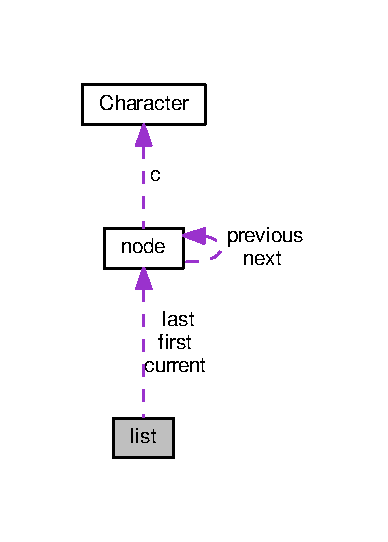
\includegraphics[width=186pt]{structlist__coll__graph}
\end{center}
\end{figure}
\subsection*{Data Fields}
\begin{DoxyCompactItemize}
\item 
\hypertarget{structlist_a02b4428208fd0060bb54d5bb726702d4}{\hyperlink{structnode}{node} $\ast$ {\bfseries first}}\label{structlist_a02b4428208fd0060bb54d5bb726702d4}

\item 
\hyperlink{structnode}{node} $\ast$ \hyperlink{structlist_a79bec8ecf9f3599d31d97683cc6f6c54}{current}
\item 
\hyperlink{structnode}{node} $\ast$ \hyperlink{structlist_a1e751cb2643f0c20321d5b233e4fdf65}{last}
\end{DoxyCompactItemize}


\subsection{Detailed Description}
the linked list that stock the ennemies 

\subsection{Field Documentation}
\hypertarget{structlist_a79bec8ecf9f3599d31d97683cc6f6c54}{\index{list@{list}!current@{current}}
\index{current@{current}!list@{list}}
\subsubsection[{current}]{\setlength{\rightskip}{0pt plus 5cm}{\bf node}$\ast$ current}}\label{structlist_a79bec8ecf9f3599d31d97683cc6f6c54}
the list's first node \hypertarget{structlist_a1e751cb2643f0c20321d5b233e4fdf65}{\index{list@{list}!last@{last}}
\index{last@{last}!list@{list}}
\subsubsection[{last}]{\setlength{\rightskip}{0pt plus 5cm}{\bf node}$\ast$ last}}\label{structlist_a1e751cb2643f0c20321d5b233e4fdf65}
the list 's current node 

The documentation for this struct was generated from the following file\-:\begin{DoxyCompactItemize}
\item 
\hyperlink{structures_8h}{structures.\-h}\end{DoxyCompactItemize}

\hypertarget{struct_map}{\subsection{Map Struct Reference}
\label{struct_map}\index{Map@{Map}}
}


{\ttfamily \#include $<$const.\-h$>$}



Collaboration diagram for Map\-:\nopagebreak
\begin{figure}[H]
\begin{center}
\leavevmode
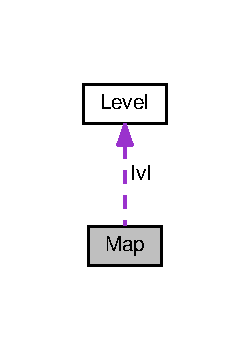
\includegraphics[width=120pt]{struct_map__coll__graph}
\end{center}
\end{figure}
\subsubsection*{Data Fields}
\begin{DoxyCompactItemize}
\item 
\hyperlink{struct_level}{Level} $\ast$ \hyperlink{struct_map_abca19b7de8e60347a507d1aeff95c764}{lvl}
\item 
int \hyperlink{struct_map_aa83bbdf2603e42824cd0bab44bf315c2}{x\-Scroll}
\item 
int \hyperlink{struct_map_ae50cb92a78d9e0a4f4bd718fc02bd294}{screen\-Width}
\item 
int \hyperlink{struct_map_a9ebc1dbd77788c4bfa27758a6725413f}{screen\-Height}
\end{DoxyCompactItemize}


\subsubsection{Detailed Description}
The map structure 

\subsubsection{Field Documentation}
\hypertarget{struct_map_abca19b7de8e60347a507d1aeff95c764}{\index{Map@{Map}!lvl@{lvl}}
\index{lvl@{lvl}!Map@{Map}}
\paragraph[{lvl}]{\setlength{\rightskip}{0pt plus 5cm}{\bf Level}$\ast$ lvl}}\label{struct_map_abca19b7de8e60347a507d1aeff95c764}
The level \hypertarget{struct_map_a9ebc1dbd77788c4bfa27758a6725413f}{\index{Map@{Map}!screen\-Height@{screen\-Height}}
\index{screen\-Height@{screen\-Height}!Map@{Map}}
\paragraph[{screen\-Height}]{\setlength{\rightskip}{0pt plus 5cm}int screen\-Height}}\label{struct_map_a9ebc1dbd77788c4bfa27758a6725413f}
The screen height \hypertarget{struct_map_ae50cb92a78d9e0a4f4bd718fc02bd294}{\index{Map@{Map}!screen\-Width@{screen\-Width}}
\index{screen\-Width@{screen\-Width}!Map@{Map}}
\paragraph[{screen\-Width}]{\setlength{\rightskip}{0pt plus 5cm}int screen\-Width}}\label{struct_map_ae50cb92a78d9e0a4f4bd718fc02bd294}
The Screen width \hypertarget{struct_map_aa83bbdf2603e42824cd0bab44bf315c2}{\index{Map@{Map}!x\-Scroll@{x\-Scroll}}
\index{x\-Scroll@{x\-Scroll}!Map@{Map}}
\paragraph[{x\-Scroll}]{\setlength{\rightskip}{0pt plus 5cm}int x\-Scroll}}\label{struct_map_aa83bbdf2603e42824cd0bab44bf315c2}
The xscroll 

The documentation for this struct was generated from the following file\-:\begin{DoxyCompactItemize}
\item 
\hyperlink{const_8h}{const.\-h}\end{DoxyCompactItemize}

\hypertarget{structnode}{\section{node Struct Reference}
\label{structnode}\index{node@{node}}
}


{\ttfamily \#include $<$structures.\-h$>$}



Collaboration diagram for node\-:
\nopagebreak
\begin{figure}[H]
\begin{center}
\leavevmode
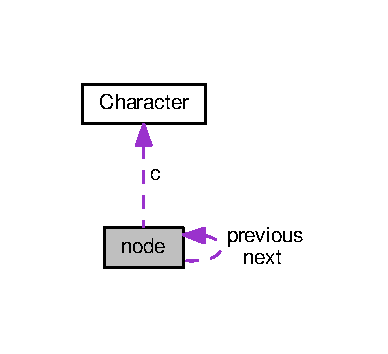
\includegraphics[width=186pt]{structnode__coll__graph}
\end{center}
\end{figure}
\subsection*{Data Fields}
\begin{DoxyCompactItemize}
\item 
\hypertarget{structnode_af76e20a507ad8fd205b860bab7ba4416}{\hyperlink{struct_character}{Character} $\ast$ {\bfseries c}}\label{structnode_af76e20a507ad8fd205b860bab7ba4416}

\item 
struct \hyperlink{structnode}{node} $\ast$ \hyperlink{structnode_a0dc1b6470487aa86d9936e3cab8b95be}{next}
\item 
struct \hyperlink{structnode}{node} $\ast$ \hyperlink{structnode_aba783da56f092df6846bd3b7b9555728}{previous}
\end{DoxyCompactItemize}


\subsection{Detailed Description}
node for the enemy list 

\subsection{Field Documentation}
\hypertarget{structnode_a0dc1b6470487aa86d9936e3cab8b95be}{\index{node@{node}!next@{next}}
\index{next@{next}!node@{node}}
\subsubsection[{next}]{\setlength{\rightskip}{0pt plus 5cm}struct {\bf node}$\ast$ next}}\label{structnode_a0dc1b6470487aa86d9936e3cab8b95be}
characater of the node \hypertarget{structnode_aba783da56f092df6846bd3b7b9555728}{\index{node@{node}!previous@{previous}}
\index{previous@{previous}!node@{node}}
\subsubsection[{previous}]{\setlength{\rightskip}{0pt plus 5cm}struct {\bf node}$\ast$ previous}}\label{structnode_aba783da56f092df6846bd3b7b9555728}
next node of the linked list 

The documentation for this struct was generated from the following file\-:\begin{DoxyCompactItemize}
\item 
\hyperlink{structures_8h}{structures.\-h}\end{DoxyCompactItemize}

\hypertarget{structplatform}{\section{platform Struct Reference}
\label{structplatform}\index{platform@{platform}}
}


{\ttfamily \#include $<$structures.\-h$>$}

\subsection*{Data Fields}
\begin{DoxyCompactItemize}
\item 
\hypertarget{structplatform_a1c7252614a33238e51edd3bbd5fa08c5}{S\-D\-L\-\_\-\-Surface $\ast$ {\bfseries sprite}}\label{structplatform_a1c7252614a33238e51edd3bbd5fa08c5}

\item 
S\-D\-L\-\_\-\-Rect \hyperlink{structplatform_a08e7ab1c2395b84bea7ca13eb99bac60}{location}
\item 
int \hyperlink{structplatform_aa91afe2b50db2f2fc786f4caf9f16f69}{x\-Min}
\item 
int \hyperlink{structplatform_af201ccbf3fe6a7e8274aa3eca22ac711}{x\-Max}
\item 
int \hyperlink{structplatform_abd0259c29e89b8f4ee318478bf207cf8}{y\-Min}
\item 
int \hyperlink{structplatform_a7ca443cbb568e95510880b6ec54dbe5e}{y\-Max}
\item 
int \hyperlink{structplatform_ac765329451135abec74c45e1897abf26}{type}
\item 
int \hyperlink{structplatform_a886d551d5381dc3e53f17825ffc51641}{direction}
\item 
int \hyperlink{structplatform_a218b4f7c6cc2681a99c23a3b089d68b1}{speed}
\end{DoxyCompactItemize}


\subsection{Detailed Description}
a mobile platform 

\subsection{Field Documentation}
\hypertarget{structplatform_a886d551d5381dc3e53f17825ffc51641}{\index{platform@{platform}!direction@{direction}}
\index{direction@{direction}!platform@{platform}}
\subsubsection[{direction}]{\setlength{\rightskip}{0pt plus 5cm}int direction}}\label{structplatform_a886d551d5381dc3e53f17825ffc51641}
0 if horizontal movement, 1 if vertical \hypertarget{structplatform_a08e7ab1c2395b84bea7ca13eb99bac60}{\index{platform@{platform}!location@{location}}
\index{location@{location}!platform@{platform}}
\subsubsection[{location}]{\setlength{\rightskip}{0pt plus 5cm}S\-D\-L\-\_\-\-Rect location}}\label{structplatform_a08e7ab1c2395b84bea7ca13eb99bac60}
the platform's sprite \hypertarget{structplatform_a218b4f7c6cc2681a99c23a3b089d68b1}{\index{platform@{platform}!speed@{speed}}
\index{speed@{speed}!platform@{platform}}
\subsubsection[{speed}]{\setlength{\rightskip}{0pt plus 5cm}int speed}}\label{structplatform_a218b4f7c6cc2681a99c23a3b089d68b1}
the platform direction \hypertarget{structplatform_ac765329451135abec74c45e1897abf26}{\index{platform@{platform}!type@{type}}
\index{type@{type}!platform@{platform}}
\subsubsection[{type}]{\setlength{\rightskip}{0pt plus 5cm}int type}}\label{structplatform_ac765329451135abec74c45e1897abf26}
y hight limit for deplacement \hypertarget{structplatform_af201ccbf3fe6a7e8274aa3eca22ac711}{\index{platform@{platform}!x\-Max@{x\-Max}}
\index{x\-Max@{x\-Max}!platform@{platform}}
\subsubsection[{x\-Max}]{\setlength{\rightskip}{0pt plus 5cm}int x\-Max}}\label{structplatform_af201ccbf3fe6a7e8274aa3eca22ac711}
x low limit for deplacement \hypertarget{structplatform_aa91afe2b50db2f2fc786f4caf9f16f69}{\index{platform@{platform}!x\-Min@{x\-Min}}
\index{x\-Min@{x\-Min}!platform@{platform}}
\subsubsection[{x\-Min}]{\setlength{\rightskip}{0pt plus 5cm}int x\-Min}}\label{structplatform_aa91afe2b50db2f2fc786f4caf9f16f69}
the platform location \hypertarget{structplatform_a7ca443cbb568e95510880b6ec54dbe5e}{\index{platform@{platform}!y\-Max@{y\-Max}}
\index{y\-Max@{y\-Max}!platform@{platform}}
\subsubsection[{y\-Max}]{\setlength{\rightskip}{0pt plus 5cm}int y\-Max}}\label{structplatform_a7ca443cbb568e95510880b6ec54dbe5e}
y hight limit for deplacement \hypertarget{structplatform_abd0259c29e89b8f4ee318478bf207cf8}{\index{platform@{platform}!y\-Min@{y\-Min}}
\index{y\-Min@{y\-Min}!platform@{platform}}
\subsubsection[{y\-Min}]{\setlength{\rightskip}{0pt plus 5cm}int y\-Min}}\label{structplatform_abd0259c29e89b8f4ee318478bf207cf8}
x hight limit for deplacement 

The documentation for this struct was generated from the following file\-:\begin{DoxyCompactItemize}
\item 
\hyperlink{structures_8h}{structures.\-h}\end{DoxyCompactItemize}

\hypertarget{structplatform_set}{\section{platform\-Set Struct Reference}
\label{structplatform_set}\index{platform\-Set@{platform\-Set}}
}


{\ttfamily \#include $<$structures.\-h$>$}



Collaboration diagram for platform\-Set\-:
\nopagebreak
\begin{figure}[H]
\begin{center}
\leavevmode
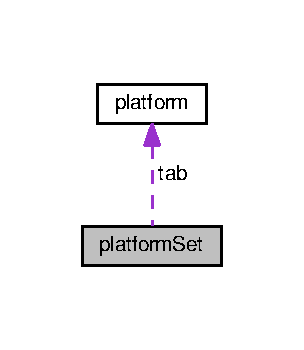
\includegraphics[width=146pt]{structplatform_set__coll__graph}
\end{center}
\end{figure}
\subsection*{Data Fields}
\begin{DoxyCompactItemize}
\item 
\hypertarget{structplatform_set_adc68016a9ab856bd20fb14c5c71c234a}{\hyperlink{structplatform}{platform} $\ast$ {\bfseries tab} \mbox{[}M\-A\-X\-\_\-\-N\-B\-\_\-\-P\-L\-A\-T\-F\-O\-R\-M\mbox{]}}\label{structplatform_set_adc68016a9ab856bd20fb14c5c71c234a}

\item 
int \hyperlink{structplatform_set_ab310c6afcc676eab3930dce2650511c0}{nb}
\end{DoxyCompactItemize}


\subsection{Detailed Description}
the set of the mobile platform 

\subsection{Field Documentation}
\hypertarget{structplatform_set_ab310c6afcc676eab3930dce2650511c0}{\index{platform\-Set@{platform\-Set}!nb@{nb}}
\index{nb@{nb}!platformSet@{platform\-Set}}
\subsubsection[{nb}]{\setlength{\rightskip}{0pt plus 5cm}int nb}}\label{structplatform_set_ab310c6afcc676eab3930dce2650511c0}
the platform set 

The documentation for this struct was generated from the following file\-:\begin{DoxyCompactItemize}
\item 
\hyperlink{structures_8h}{structures.\-h}\end{DoxyCompactItemize}

\hypertarget{struct_player}{\subsection{Player Struct Reference}
\label{struct_player}\index{Player@{Player}}
}


{\ttfamily \#include $<$structures.\-h$>$}

\subsubsection*{Data Fields}
\begin{DoxyCompactItemize}
\item 
int \hyperlink{struct_player_a239aaece8decb78587f72db6166743ca}{level\-Max}
\item 
int \hyperlink{struct_player_a803fd7edf0558a9e0dc73e6351ad85d0}{nb\-Projectile}
\item 
int \hyperlink{struct_player_ae4069fd5e08497b888237e5eb9f2e4ad}{nb\-Lifes}
\item 
int \hyperlink{struct_player_a90f72e24f08427f541b92bfc5a7982d3}{nb\-Coins}
\end{DoxyCompactItemize}


\subsubsection{Detailed Description}
The player 

\subsubsection{Field Documentation}
\hypertarget{struct_player_a239aaece8decb78587f72db6166743ca}{\index{Player@{Player}!level\-Max@{level\-Max}}
\index{level\-Max@{level\-Max}!Player@{Player}}
\paragraph[{level\-Max}]{\setlength{\rightskip}{0pt plus 5cm}int level\-Max}}\label{struct_player_a239aaece8decb78587f72db6166743ca}
The level max \hypertarget{struct_player_a90f72e24f08427f541b92bfc5a7982d3}{\index{Player@{Player}!nb\-Coins@{nb\-Coins}}
\index{nb\-Coins@{nb\-Coins}!Player@{Player}}
\paragraph[{nb\-Coins}]{\setlength{\rightskip}{0pt plus 5cm}int nb\-Coins}}\label{struct_player_a90f72e24f08427f541b92bfc5a7982d3}
The number of coins \hypertarget{struct_player_ae4069fd5e08497b888237e5eb9f2e4ad}{\index{Player@{Player}!nb\-Lifes@{nb\-Lifes}}
\index{nb\-Lifes@{nb\-Lifes}!Player@{Player}}
\paragraph[{nb\-Lifes}]{\setlength{\rightskip}{0pt plus 5cm}int nb\-Lifes}}\label{struct_player_ae4069fd5e08497b888237e5eb9f2e4ad}
The number of life \hypertarget{struct_player_a803fd7edf0558a9e0dc73e6351ad85d0}{\index{Player@{Player}!nb\-Projectile@{nb\-Projectile}}
\index{nb\-Projectile@{nb\-Projectile}!Player@{Player}}
\paragraph[{nb\-Projectile}]{\setlength{\rightskip}{0pt plus 5cm}int nb\-Projectile}}\label{struct_player_a803fd7edf0558a9e0dc73e6351ad85d0}
The number of projectile 

The documentation for this struct was generated from the following file\-:\begin{DoxyCompactItemize}
\item 
\hyperlink{structures_8h}{structures.\-h}\end{DoxyCompactItemize}

\hypertarget{structprojectile}{\section{projectile Struct Reference}
\label{structprojectile}\index{projectile@{projectile}}
}


{\ttfamily \#include $<$structures.\-h$>$}

\subsection*{Data Fields}
\begin{DoxyCompactItemize}
\item 
\hypertarget{structprojectile_a1c7252614a33238e51edd3bbd5fa08c5}{S\-D\-L\-\_\-\-Surface $\ast$ {\bfseries sprite}}\label{structprojectile_a1c7252614a33238e51edd3bbd5fa08c5}

\item 
S\-D\-L\-\_\-\-Rect \hyperlink{structprojectile_a08e7ab1c2395b84bea7ca13eb99bac60}{location}
\item 
int \hyperlink{structprojectile_a886d551d5381dc3e53f17825ffc51641}{direction}
\item 
int \hyperlink{structprojectile_a130dff78b354d57d5b6dadcad3e597ef}{from\-N\-P\-C}
\end{DoxyCompactItemize}


\subsection{Detailed Description}
a projectile structure 

\subsection{Field Documentation}
\hypertarget{structprojectile_a886d551d5381dc3e53f17825ffc51641}{\index{projectile@{projectile}!direction@{direction}}
\index{direction@{direction}!projectile@{projectile}}
\subsubsection[{direction}]{\setlength{\rightskip}{0pt plus 5cm}int direction}}\label{structprojectile_a886d551d5381dc3e53f17825ffc51641}
the platform location \hypertarget{structprojectile_a130dff78b354d57d5b6dadcad3e597ef}{\index{projectile@{projectile}!from\-N\-P\-C@{from\-N\-P\-C}}
\index{from\-N\-P\-C@{from\-N\-P\-C}!projectile@{projectile}}
\subsubsection[{from\-N\-P\-C}]{\setlength{\rightskip}{0pt plus 5cm}int from\-N\-P\-C}}\label{structprojectile_a130dff78b354d57d5b6dadcad3e597ef}
the platform direction \hypertarget{structprojectile_a08e7ab1c2395b84bea7ca13eb99bac60}{\index{projectile@{projectile}!location@{location}}
\index{location@{location}!projectile@{projectile}}
\subsubsection[{location}]{\setlength{\rightskip}{0pt plus 5cm}S\-D\-L\-\_\-\-Rect location}}\label{structprojectile_a08e7ab1c2395b84bea7ca13eb99bac60}
the platform's sprite 

The documentation for this struct was generated from the following file\-:\begin{DoxyCompactItemize}
\item 
\hyperlink{structures_8h}{structures.\-h}\end{DoxyCompactItemize}

\hypertarget{structprojectile_set}{\subsection{projectile\-Set Struct Reference}
\label{structprojectile_set}\index{projectile\-Set@{projectile\-Set}}
}


{\ttfamily \#include $<$structures.\-h$>$}



Collaboration diagram for projectile\-Set\-:
\nopagebreak
\begin{figure}[H]
\begin{center}
\leavevmode
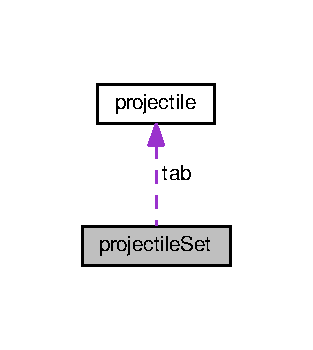
\includegraphics[width=150pt]{structprojectile_set__coll__graph}
\end{center}
\end{figure}
\subsubsection*{Data Fields}
\begin{DoxyCompactItemize}
\item 
\hyperlink{structprojectile}{projectile} $\ast$ \hyperlink{structprojectile_set_ac4cbcd75bc678f0ad2b2d416ce87dc6d}{tab} \mbox{[}\hyperlink{const_8h_a180d2c389d68d43eb0e3df2d573fecf4}{M\-A\-X\-\_\-\-N\-B\-\_\-\-P\-R\-O\-J\-E\-C\-T\-I\-L\-E}\mbox{]}
\item 
int \hyperlink{structprojectile_set_ab310c6afcc676eab3930dce2650511c0}{nb}
\item 
int \hyperlink{structprojectile_set_accfd9d1d6194770a3368821b58ffc3b6}{projectile\-Thrown}
\end{DoxyCompactItemize}


\subsubsection{Detailed Description}
the set of the projectiles 

\subsubsection{Field Documentation}
\hypertarget{structprojectile_set_ab310c6afcc676eab3930dce2650511c0}{\index{projectile\-Set@{projectile\-Set}!nb@{nb}}
\index{nb@{nb}!projectileSet@{projectile\-Set}}
\paragraph[{nb}]{\setlength{\rightskip}{0pt plus 5cm}int nb}}\label{structprojectile_set_ab310c6afcc676eab3930dce2650511c0}
the number of projectiles on the map \hypertarget{structprojectile_set_accfd9d1d6194770a3368821b58ffc3b6}{\index{projectile\-Set@{projectile\-Set}!projectile\-Thrown@{projectile\-Thrown}}
\index{projectile\-Thrown@{projectile\-Thrown}!projectileSet@{projectile\-Set}}
\paragraph[{projectile\-Thrown}]{\setlength{\rightskip}{0pt plus 5cm}int projectile\-Thrown}}\label{structprojectile_set_accfd9d1d6194770a3368821b58ffc3b6}
indicates if a projectile has been thrown by the player and the key wasn't released yet \hypertarget{structprojectile_set_ac4cbcd75bc678f0ad2b2d416ce87dc6d}{\index{projectile\-Set@{projectile\-Set}!tab@{tab}}
\index{tab@{tab}!projectileSet@{projectile\-Set}}
\paragraph[{tab}]{\setlength{\rightskip}{0pt plus 5cm}{\bf projectile}$\ast$ tab\mbox{[}{\bf M\-A\-X\-\_\-\-N\-B\-\_\-\-P\-R\-O\-J\-E\-C\-T\-I\-L\-E}\mbox{]}}}\label{structprojectile_set_ac4cbcd75bc678f0ad2b2d416ce87dc6d}
the projectile set 

The documentation for this struct was generated from the following file\-:\begin{DoxyCompactItemize}
\item 
\hyperlink{structures_8h}{structures.\-h}\end{DoxyCompactItemize}

\hypertarget{struct_sound}{\subsection{Sound Struct Reference}
\label{struct_sound}\index{Sound@{Sound}}
}


{\ttfamily \#include $<$sound.\-h$>$}

\subsubsection*{Data Fields}
\begin{DoxyCompactItemize}
\item 
\hypertarget{struct_sound_ae043bb23ee313709e1c605dd6c06d317}{F\-M\-O\-D\-\_\-\-S\-Y\-S\-T\-E\-M $\ast$ {\bfseries sys}}\label{struct_sound_ae043bb23ee313709e1c605dd6c06d317}

\item 
F\-M\-O\-D\-\_\-\-C\-H\-A\-N\-N\-E\-L $\ast$ \hyperlink{struct_sound_acca26c408c6140c8cdc0d8f49d31ad4a}{music}
\item 
F\-M\-O\-D\-\_\-\-C\-H\-A\-N\-N\-E\-L $\ast$ \hyperlink{struct_sound_a259d72174e26b5bb58146484cd54c1c8}{fx}
\item 
F\-M\-O\-D\-\_\-\-S\-O\-U\-N\-D $\ast$ \hyperlink{struct_sound_a1051e4654836160d314f8d49fe85ae77}{msc\-Sound}
\item 
F\-M\-O\-D\-\_\-\-S\-O\-U\-N\-D $\ast$ \hyperlink{struct_sound_a38b0d95773369da732eb81a289b52940}{fx\-Sound}
\item 
float \hyperlink{struct_sound_a6f06b572245c72c79f052b7efb89dc3b}{music\-Volume}
\item 
float \hyperlink{struct_sound_aedb4246a8bbae1c53f2f29572674b054}{fx\-Volume}
\end{DoxyCompactItemize}


\subsubsection{Detailed Description}
the sound gestion structure 

\subsubsection{Field Documentation}
\hypertarget{struct_sound_a259d72174e26b5bb58146484cd54c1c8}{\index{Sound@{Sound}!fx@{fx}}
\index{fx@{fx}!Sound@{Sound}}
\paragraph[{fx}]{\setlength{\rightskip}{0pt plus 5cm}F\-M\-O\-D\-\_\-\-C\-H\-A\-N\-N\-E\-L$\ast$ fx}}\label{struct_sound_a259d72174e26b5bb58146484cd54c1c8}
the music channel \hypertarget{struct_sound_a38b0d95773369da732eb81a289b52940}{\index{Sound@{Sound}!fx\-Sound@{fx\-Sound}}
\index{fx\-Sound@{fx\-Sound}!Sound@{Sound}}
\paragraph[{fx\-Sound}]{\setlength{\rightskip}{0pt plus 5cm}F\-M\-O\-D\-\_\-\-S\-O\-U\-N\-D$\ast$ fx\-Sound}}\label{struct_sound_a38b0d95773369da732eb81a289b52940}
the music sound \hypertarget{struct_sound_aedb4246a8bbae1c53f2f29572674b054}{\index{Sound@{Sound}!fx\-Volume@{fx\-Volume}}
\index{fx\-Volume@{fx\-Volume}!Sound@{Sound}}
\paragraph[{fx\-Volume}]{\setlength{\rightskip}{0pt plus 5cm}float fx\-Volume}}\label{struct_sound_aedb4246a8bbae1c53f2f29572674b054}
the music volume \hypertarget{struct_sound_a1051e4654836160d314f8d49fe85ae77}{\index{Sound@{Sound}!msc\-Sound@{msc\-Sound}}
\index{msc\-Sound@{msc\-Sound}!Sound@{Sound}}
\paragraph[{msc\-Sound}]{\setlength{\rightskip}{0pt plus 5cm}F\-M\-O\-D\-\_\-\-S\-O\-U\-N\-D$\ast$ msc\-Sound}}\label{struct_sound_a1051e4654836160d314f8d49fe85ae77}
the effects channel \hypertarget{struct_sound_acca26c408c6140c8cdc0d8f49d31ad4a}{\index{Sound@{Sound}!music@{music}}
\index{music@{music}!Sound@{Sound}}
\paragraph[{music}]{\setlength{\rightskip}{0pt plus 5cm}F\-M\-O\-D\-\_\-\-C\-H\-A\-N\-N\-E\-L$\ast$ music}}\label{struct_sound_acca26c408c6140c8cdc0d8f49d31ad4a}
the sound system \hypertarget{struct_sound_a6f06b572245c72c79f052b7efb89dc3b}{\index{Sound@{Sound}!music\-Volume@{music\-Volume}}
\index{music\-Volume@{music\-Volume}!Sound@{Sound}}
\paragraph[{music\-Volume}]{\setlength{\rightskip}{0pt plus 5cm}float music\-Volume}}\label{struct_sound_a6f06b572245c72c79f052b7efb89dc3b}
the effects sound 

The documentation for this struct was generated from the following file\-:\begin{DoxyCompactItemize}
\item 
\hyperlink{sound_8h}{sound.\-h}\end{DoxyCompactItemize}

\section{File Documentation}
\hypertarget{character_8c}{\subsection{character.\-c File Reference}
\label{character_8c}\index{character.\-c@{character.\-c}}
}


manipulate character  


{\ttfamily \#include \char`\"{}character.\-h\char`\"{}}\\*
\subsubsection*{Functions}
\begin{DoxyCompactItemize}
\item 
\hyperlink{struct_character}{Character} $\ast$ \hyperlink{character_8c_a2960e507261021990900980ed217b418}{create\-Character} (char $\ast$tile, int x, int y, int npc, int nb\-Projectile, int nb\-Coins, int nb\-Lifes)
\item 
void \hyperlink{character_8c_a3cace1cd02fa4987839238e5d4f79796}{free\-Characters} (\hyperlink{struct_character}{Character} $\ast$c)
\item 
int \hyperlink{character_8c_afee02e189e4fc6308f0359f0afe747cb}{move\-Character} (\hyperlink{struct_character}{Character} $\ast$c, float move\-\_\-left, float move\-\_\-right, int jump, \hyperlink{struct_map}{Map} $\ast$m, float $\ast$speed, \hyperlink{structlist}{list} $\ast$l, \hyperlink{struct_sound}{Sound} $\ast$sound\-\_\-sys, \hyperlink{structplatform_set}{platform\-Set} $\ast$ps)
\item 
int \hyperlink{character_8c_af15e182c04b17ce9a3d16872f2bf4f49}{try\-Movement} (\hyperlink{struct_character}{Character} $\ast$c, int vx, int vy, \hyperlink{struct_map}{Map} $\ast$m, \hyperlink{structlist}{list} $\ast$l, \hyperlink{structplatform_set}{platform\-Set} $\ast$ps, \hyperlink{struct_sound}{Sound} $\ast$sound\-\_\-sys)
\item 
int \hyperlink{character_8c_a7b6d5ab652a57c5d6ffbaea628164402}{collision\-Sprite} (S\-D\-L\-\_\-\-Rect s1, S\-D\-L\-\_\-\-Rect s2)
\item 
void \hyperlink{character_8c_a3c4b84a9d7123af243336f3540d2ae83}{blit\-Character} (S\-D\-L\-\_\-\-Surface $\ast$screen, \hyperlink{struct_character}{Character} $\ast$c, \hyperlink{struct_map}{Map} $\ast$m)
\item 
void \hyperlink{character_8c_a780616fe53145812a634dcf5e4f20959}{presise\-Move\-Character} (\hyperlink{struct_character}{Character} $\ast$c, int vx, int vy, \hyperlink{struct_map}{Map} $\ast$m, \hyperlink{structlist}{list} $\ast$l, \hyperlink{structplatform_set}{platform\-Set} $\ast$ps)
\item 
int \hyperlink{character_8c_a81dc963e2a308d0e3e627b7652aa7489}{check\-Wall} (\hyperlink{struct_character}{Character} $\ast$c, \hyperlink{struct_map}{Map} $\ast$m)
\item 
int \hyperlink{character_8c_aea69b279f0dc778dde496ea610f1aa82}{check\-Fall} (\hyperlink{struct_character}{Character} $\ast$c, \hyperlink{struct_map}{Map} $\ast$m, \hyperlink{structplatform_set}{platform\-Set} $\ast$ps)
\end{DoxyCompactItemize}


\subsubsection{Detailed Description}
manipulate character \begin{DoxyAuthor}{Author}
Xavier C\-O\-P\-O\-N\-E\-T 
\end{DoxyAuthor}
\begin{DoxyDate}{Date}
2014-\/02-\/27 
\end{DoxyDate}


\subsubsection{Function Documentation}
\hypertarget{character_8c_a3c4b84a9d7123af243336f3540d2ae83}{\index{character.\-c@{character.\-c}!blit\-Character@{blit\-Character}}
\index{blit\-Character@{blit\-Character}!character.c@{character.\-c}}
\paragraph[{blit\-Character}]{\setlength{\rightskip}{0pt plus 5cm}void blit\-Character (
\begin{DoxyParamCaption}
\item[{S\-D\-L\-\_\-\-Surface $\ast$}]{screen, }
\item[{{\bf Character} $\ast$}]{c, }
\item[{{\bf Map} $\ast$}]{m}
\end{DoxyParamCaption}
)}}\label{character_8c_a3c4b84a9d7123af243336f3540d2ae83}
blit the character 
\begin{DoxyParams}[1]{Parameters}
\mbox{\tt in,out}  & {\em screen} & game screen \\
\hline
\mbox{\tt in}  & {\em c} & the character \\
\hline
\mbox{\tt in}  & {\em m} & game map \\
\hline
\end{DoxyParams}
\hypertarget{character_8c_aea69b279f0dc778dde496ea610f1aa82}{\index{character.\-c@{character.\-c}!check\-Fall@{check\-Fall}}
\index{check\-Fall@{check\-Fall}!character.c@{character.\-c}}
\paragraph[{check\-Fall}]{\setlength{\rightskip}{0pt plus 5cm}int check\-Fall (
\begin{DoxyParamCaption}
\item[{{\bf Character} $\ast$}]{c, }
\item[{{\bf Map} $\ast$}]{m, }
\item[{{\bf platform\-Set} $\ast$}]{ps}
\end{DoxyParamCaption}
)}}\label{character_8c_aea69b279f0dc778dde496ea610f1aa82}
tests if the character's futur position is over a void tile 
\begin{DoxyParams}[1]{Parameters}
\mbox{\tt in}  & {\em c} & the monster/character to be tested \\
\hline
\mbox{\tt in}  & {\em m} & the game map \\
\hline
\mbox{\tt in}  & {\em ps} & the platform set \\
\hline
\end{DoxyParams}
\begin{DoxyReturn}{Returns}
1 if void tile, 0 if not 
\end{DoxyReturn}
\hypertarget{character_8c_a81dc963e2a308d0e3e627b7652aa7489}{\index{character.\-c@{character.\-c}!check\-Wall@{check\-Wall}}
\index{check\-Wall@{check\-Wall}!character.c@{character.\-c}}
\paragraph[{check\-Wall}]{\setlength{\rightskip}{0pt plus 5cm}int check\-Wall (
\begin{DoxyParamCaption}
\item[{{\bf Character} $\ast$}]{c, }
\item[{{\bf Map} $\ast$}]{m}
\end{DoxyParamCaption}
)}}\label{character_8c_a81dc963e2a308d0e3e627b7652aa7489}
tests if the character's futur position is next to a wall tile 
\begin{DoxyParams}[1]{Parameters}
\mbox{\tt in}  & {\em c} & the monster/character to be tested \\
\hline
\mbox{\tt in}  & {\em m} & the game map \\
\hline
\end{DoxyParams}
\begin{DoxyReturn}{Returns}
1 if wall tile, 0 if not 
\end{DoxyReturn}
\hypertarget{character_8c_a7b6d5ab652a57c5d6ffbaea628164402}{\index{character.\-c@{character.\-c}!collision\-Sprite@{collision\-Sprite}}
\index{collision\-Sprite@{collision\-Sprite}!character.c@{character.\-c}}
\paragraph[{collision\-Sprite}]{\setlength{\rightskip}{0pt plus 5cm}int collision\-Sprite (
\begin{DoxyParamCaption}
\item[{S\-D\-L\-\_\-\-Rect}]{s1, }
\item[{S\-D\-L\-\_\-\-Rect}]{s2}
\end{DoxyParamCaption}
)}}\label{character_8c_a7b6d5ab652a57c5d6ffbaea628164402}
int \hyperlink{character_8h_a7b6d5ab652a57c5d6ffbaea628164402}{collision\-Sprite(\-S\-D\-L\-\_\-\-Rect s1, S\-D\-L\-\_\-\-Rect s2)} determine if there is a collision beteewen two sprites 
\begin{DoxyParams}[1]{Parameters}
\mbox{\tt in}  & {\em s1} & the first sprite \\
\hline
\mbox{\tt in}  & {\em s2} & the second sprite \\
\hline
\end{DoxyParams}
\begin{DoxyReturn}{Returns}
3 if there is a collision and s1 is below s2, 2 if there is a collision and s1 is over s2, 0 if there is no collision 
\end{DoxyReturn}
\hypertarget{character_8c_a2960e507261021990900980ed217b418}{\index{character.\-c@{character.\-c}!create\-Character@{create\-Character}}
\index{create\-Character@{create\-Character}!character.c@{character.\-c}}
\paragraph[{create\-Character}]{\setlength{\rightskip}{0pt plus 5cm}{\bf Character} $\ast$ create\-Character (
\begin{DoxyParamCaption}
\item[{char $\ast$}]{tile, }
\item[{int}]{x, }
\item[{int}]{y, }
\item[{int}]{npc, }
\item[{int}]{nb\-Projectile, }
\item[{int}]{nb\-Coins, }
\item[{int}]{nb\-Lifes}
\end{DoxyParamCaption}
)}}\label{character_8c_a2960e507261021990900980ed217b418}
create a character 
\begin{DoxyParams}[1]{Parameters}
\mbox{\tt in}  & {\em tile} & character tile\-Set address \\
\hline
\mbox{\tt in}  & {\em x} & character's x location \\
\hline
\mbox{\tt in}  & {\em y} & character's y location \\
\hline
\mbox{\tt in}  & {\em npc} & type of npc if creating a npc, 0 if not \\
\hline
\mbox{\tt in}  & {\em nb\-Projectile} & the number of projectiles the character has \\
\hline
\mbox{\tt in}  & {\em nb\-Coins} & the number of coins the character has \\
\hline
\mbox{\tt in}  & {\em nb\-Lifes} & the number of life the character has \\
\hline
\end{DoxyParams}
\begin{DoxyReturn}{Returns}
character structure pointer 
\end{DoxyReturn}


Here is the call graph for this function\-:
\nopagebreak
\begin{figure}[H]
\begin{center}
\leavevmode
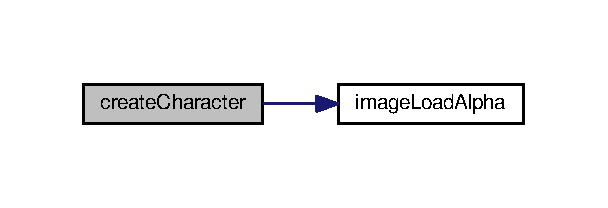
\includegraphics[width=292pt]{character_8c_a2960e507261021990900980ed217b418_cgraph}
\end{center}
\end{figure}


\hypertarget{character_8c_a3cace1cd02fa4987839238e5d4f79796}{\index{character.\-c@{character.\-c}!free\-Characters@{free\-Characters}}
\index{free\-Characters@{free\-Characters}!character.c@{character.\-c}}
\paragraph[{free\-Characters}]{\setlength{\rightskip}{0pt plus 5cm}void free\-Characters (
\begin{DoxyParamCaption}
\item[{{\bf Character} $\ast$}]{c}
\end{DoxyParamCaption}
)}}\label{character_8c_a3cace1cd02fa4987839238e5d4f79796}
Free a character 
\begin{DoxyParams}[1]{Parameters}
\mbox{\tt in,out}  & {\em c} & the character \\
\hline
\end{DoxyParams}
\hypertarget{character_8c_afee02e189e4fc6308f0359f0afe747cb}{\index{character.\-c@{character.\-c}!move\-Character@{move\-Character}}
\index{move\-Character@{move\-Character}!character.c@{character.\-c}}
\paragraph[{move\-Character}]{\setlength{\rightskip}{0pt plus 5cm}int move\-Character (
\begin{DoxyParamCaption}
\item[{{\bf Character} $\ast$}]{c, }
\item[{float}]{move\-\_\-left, }
\item[{float}]{move\-\_\-right, }
\item[{int}]{jump, }
\item[{{\bf Map} $\ast$}]{m, }
\item[{float $\ast$}]{speed, }
\item[{{\bf list} $\ast$}]{l, }
\item[{{\bf Sound} $\ast$}]{sound\-\_\-sys, }
\item[{{\bf platform\-Set} $\ast$}]{ps}
\end{DoxyParamCaption}
)}}\label{character_8c_afee02e189e4fc6308f0359f0afe747cb}
move player according to the direction 
\begin{DoxyParams}[1]{Parameters}
\mbox{\tt in,out}  & {\em c} & the character \\
\hline
\mbox{\tt in}  & {\em move\-\_\-left} & indicates if must go to the left \\
\hline
\mbox{\tt in}  & {\em move\-\_\-right} & indicates if must go to the right \\
\hline
\mbox{\tt in}  & {\em jump} & indicates if must jump \\
\hline
\mbox{\tt in}  & {\em m} & level map \\
\hline
\mbox{\tt in}  & {\em speed} & movement speed \\
\hline
\mbox{\tt in,out}  & {\em l} & the enemy list \\
\hline
\mbox{\tt out}  & {\em sound\-\_\-sys} & the sound system \\
\hline
\mbox{\tt out}  & {\em ps} & the platform set \\
\hline
\end{DoxyParams}
\begin{DoxyReturn}{Returns}
1 if character was moved without using the precise movement function, 0 if not 
\end{DoxyReturn}


Here is the call graph for this function\-:
\nopagebreak
\begin{figure}[H]
\begin{center}
\leavevmode
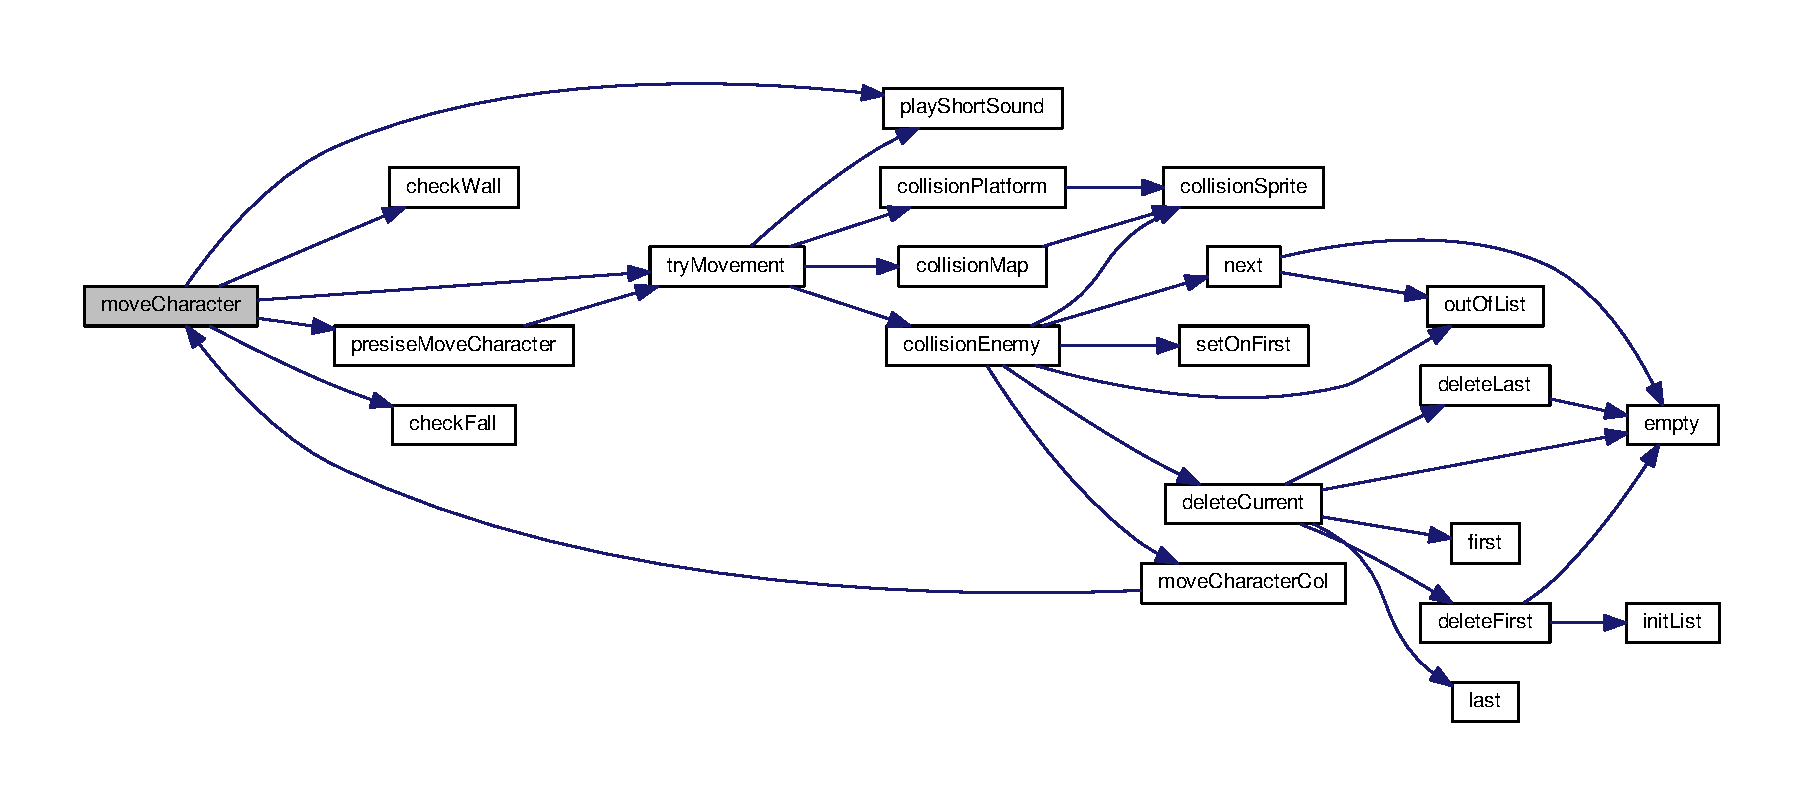
\includegraphics[width=350pt]{character_8c_afee02e189e4fc6308f0359f0afe747cb_cgraph}
\end{center}
\end{figure}


\hypertarget{character_8c_a780616fe53145812a634dcf5e4f20959}{\index{character.\-c@{character.\-c}!presise\-Move\-Character@{presise\-Move\-Character}}
\index{presise\-Move\-Character@{presise\-Move\-Character}!character.c@{character.\-c}}
\paragraph[{presise\-Move\-Character}]{\setlength{\rightskip}{0pt plus 5cm}void presise\-Move\-Character (
\begin{DoxyParamCaption}
\item[{{\bf Character} $\ast$}]{c, }
\item[{int}]{vx, }
\item[{int}]{vy, }
\item[{{\bf Map} $\ast$}]{m, }
\item[{{\bf list} $\ast$}]{l, }
\item[{{\bf platform\-Set} $\ast$}]{ps}
\end{DoxyParamCaption}
)}}\label{character_8c_a780616fe53145812a634dcf5e4f20959}
make a more presise move of a character if he can still move but the distance between it and the obstacle is less than its speed 
\begin{DoxyParams}[1]{Parameters}
\mbox{\tt in,out}  & {\em c} & the charactere \\
\hline
\mbox{\tt in}  & {\em m} & the map \\
\hline
\mbox{\tt in}  & {\em vx} & the horizontal component of the movement vector \\
\hline
\mbox{\tt in}  & {\em vy} & the vertical component of the movement vector \\
\hline
\mbox{\tt in,out}  & {\em l} & the enemy list \\
\hline
\mbox{\tt out}  & {\em ps} & the platform set \\
\hline
\end{DoxyParams}


Here is the call graph for this function\-:
\nopagebreak
\begin{figure}[H]
\begin{center}
\leavevmode
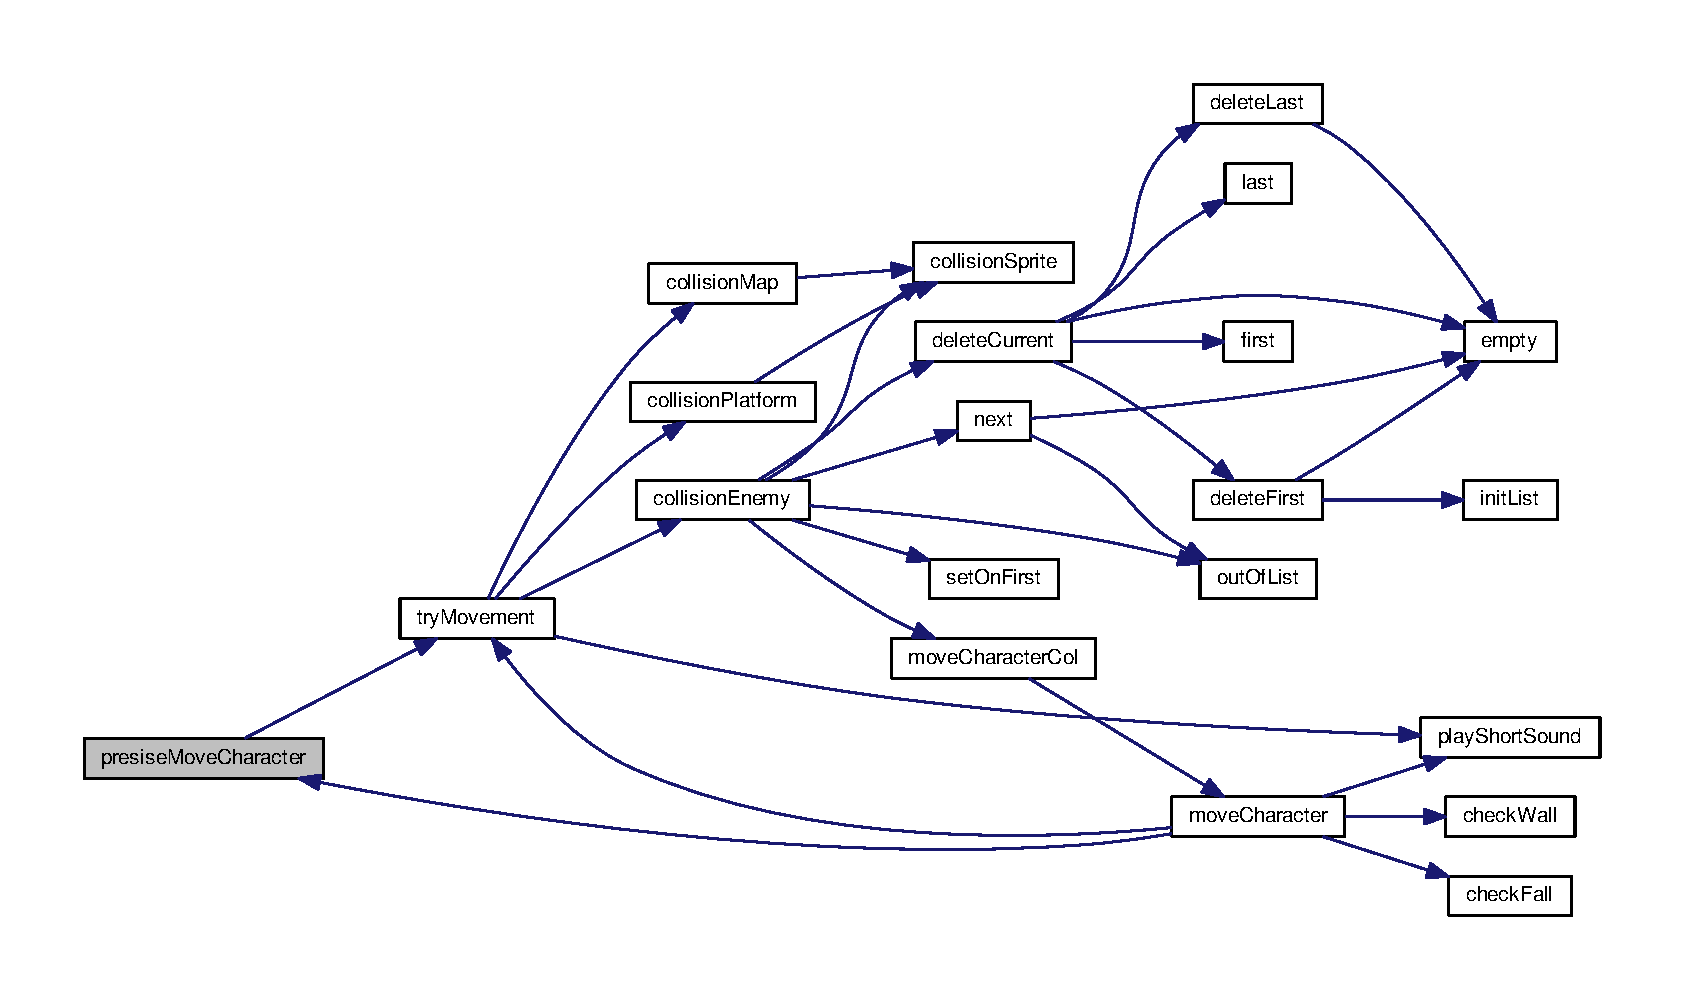
\includegraphics[width=350pt]{character_8c_a780616fe53145812a634dcf5e4f20959_cgraph}
\end{center}
\end{figure}


\hypertarget{character_8c_af15e182c04b17ce9a3d16872f2bf4f49}{\index{character.\-c@{character.\-c}!try\-Movement@{try\-Movement}}
\index{try\-Movement@{try\-Movement}!character.c@{character.\-c}}
\paragraph[{try\-Movement}]{\setlength{\rightskip}{0pt plus 5cm}int try\-Movement (
\begin{DoxyParamCaption}
\item[{{\bf Character} $\ast$}]{c, }
\item[{int}]{vx, }
\item[{int}]{vy, }
\item[{{\bf Map} $\ast$}]{m, }
\item[{{\bf list} $\ast$}]{l, }
\item[{{\bf platform\-Set} $\ast$}]{ps, }
\item[{{\bf Sound} $\ast$}]{sound\-\_\-sys}
\end{DoxyParamCaption}
)}}\label{character_8c_af15e182c04b17ce9a3d16872f2bf4f49}
try to move a character 
\begin{DoxyParams}[1]{Parameters}
\mbox{\tt in,out}  & {\em c} & the character \\
\hline
\mbox{\tt in}  & {\em vx} & the horizontal component of the movement vector \\
\hline
\mbox{\tt in}  & {\em vy} & the vertical component of the movement vector \\
\hline
\mbox{\tt in}  & {\em m} & the map the character is on \\
\hline
\mbox{\tt in,out}  & {\em l} & the enemy list \\
\hline
\mbox{\tt out}  & {\em ps} & the platform set \\
\hline
\mbox{\tt out}  & {\em sound\-\_\-sys} & the game sound system \\
\hline
\end{DoxyParams}
\begin{DoxyReturn}{Returns}
1 if the character can be moved, 0 if not 
\end{DoxyReturn}


Here is the call graph for this function\-:
\nopagebreak
\begin{figure}[H]
\begin{center}
\leavevmode
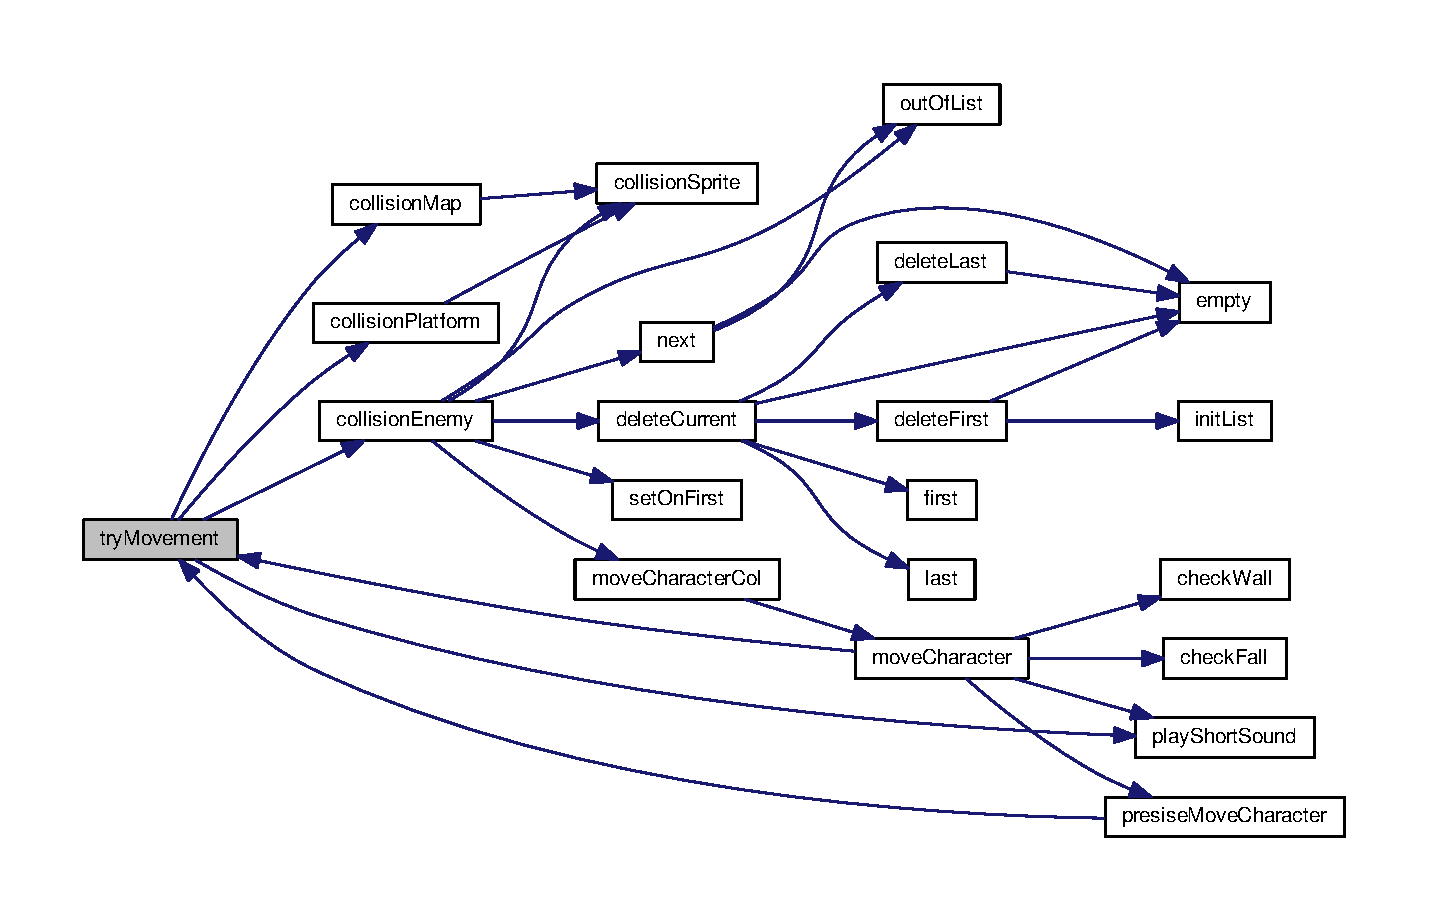
\includegraphics[width=350pt]{character_8c_af15e182c04b17ce9a3d16872f2bf4f49_cgraph}
\end{center}
\end{figure}



\hypertarget{character_8h}{\section{character.\-h File Reference}
\label{character_8h}\index{character.\-h@{character.\-h}}
}


header de \hyperlink{character_8c}{character.\-c}  


{\ttfamily \#include \char`\"{}const.\-h\char`\"{}}\\*
{\ttfamily \#include $<$stdlib.\-h$>$}\\*
{\ttfamily \#include $<$stdio.\-h$>$}\\*
{\ttfamily \#include $<$errno.\-h$>$}\\*
{\ttfamily \#include $<$S\-D\-L/\-S\-D\-L.\-h$>$}\\*
{\ttfamily \#include $<$S\-D\-L/\-S\-D\-L\-\_\-image.\-h$>$}\\*
{\ttfamily \#include \char`\"{}file\-\_\-level.\-h\char`\"{}}\\*
{\ttfamily \#include \char`\"{}share.\-h\char`\"{}}\\*
{\ttfamily \#include \char`\"{}map.\-h\char`\"{}}\\*
{\ttfamily \#include \char`\"{}structures.\-h\char`\"{}}\\*
{\ttfamily \#include \char`\"{}image.\-h\char`\"{}}\\*
{\ttfamily \#include \char`\"{}enemies.\-h\char`\"{}}\\*
{\ttfamily \#include \char`\"{}mobile\-\_\-platform.\-h\char`\"{}}\\*
{\ttfamily \#include \char`\"{}sound.\-h\char`\"{}}\\*
Include dependency graph for character.\-h\-:
\nopagebreak
\begin{figure}[H]
\begin{center}
\leavevmode
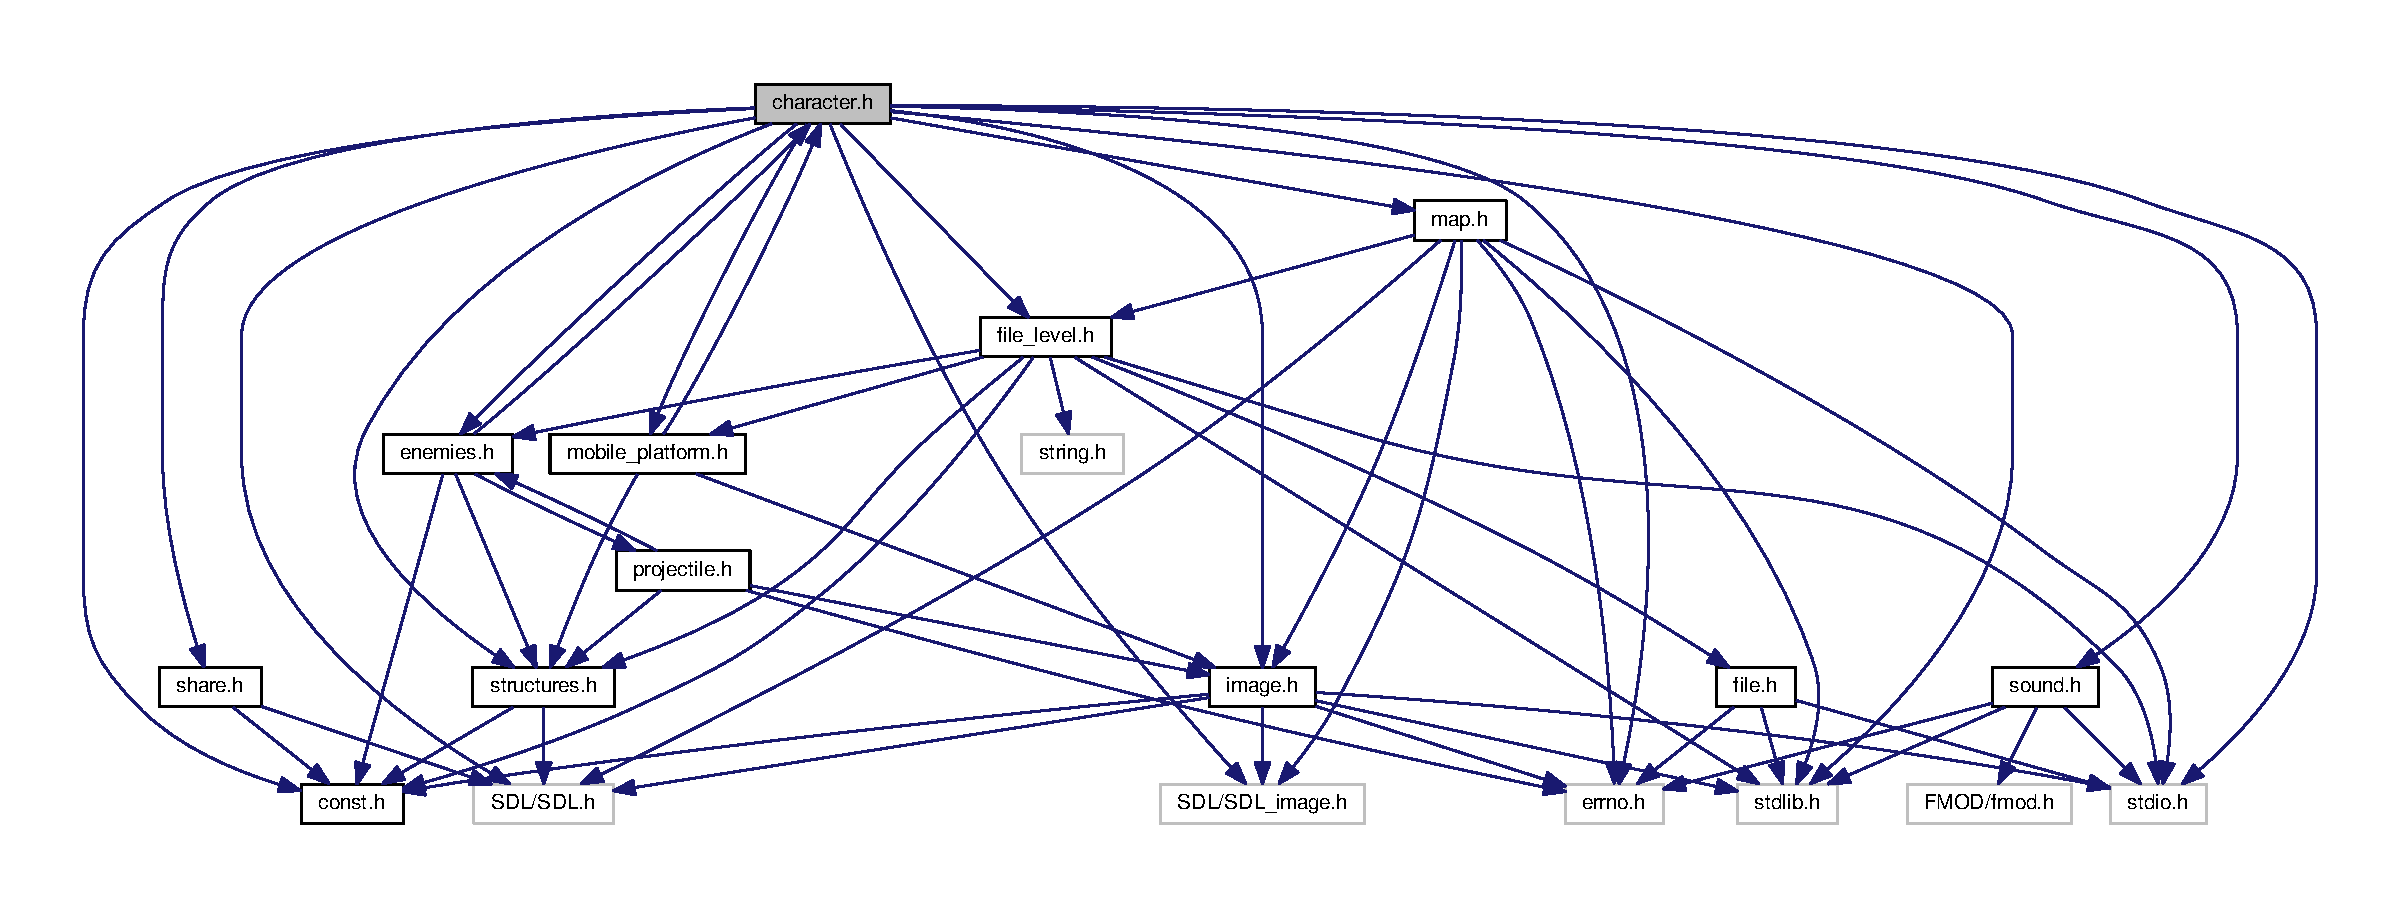
\includegraphics[width=350pt]{character_8h__incl}
\end{center}
\end{figure}
This graph shows which files directly or indirectly include this file\-:
\nopagebreak
\begin{figure}[H]
\begin{center}
\leavevmode
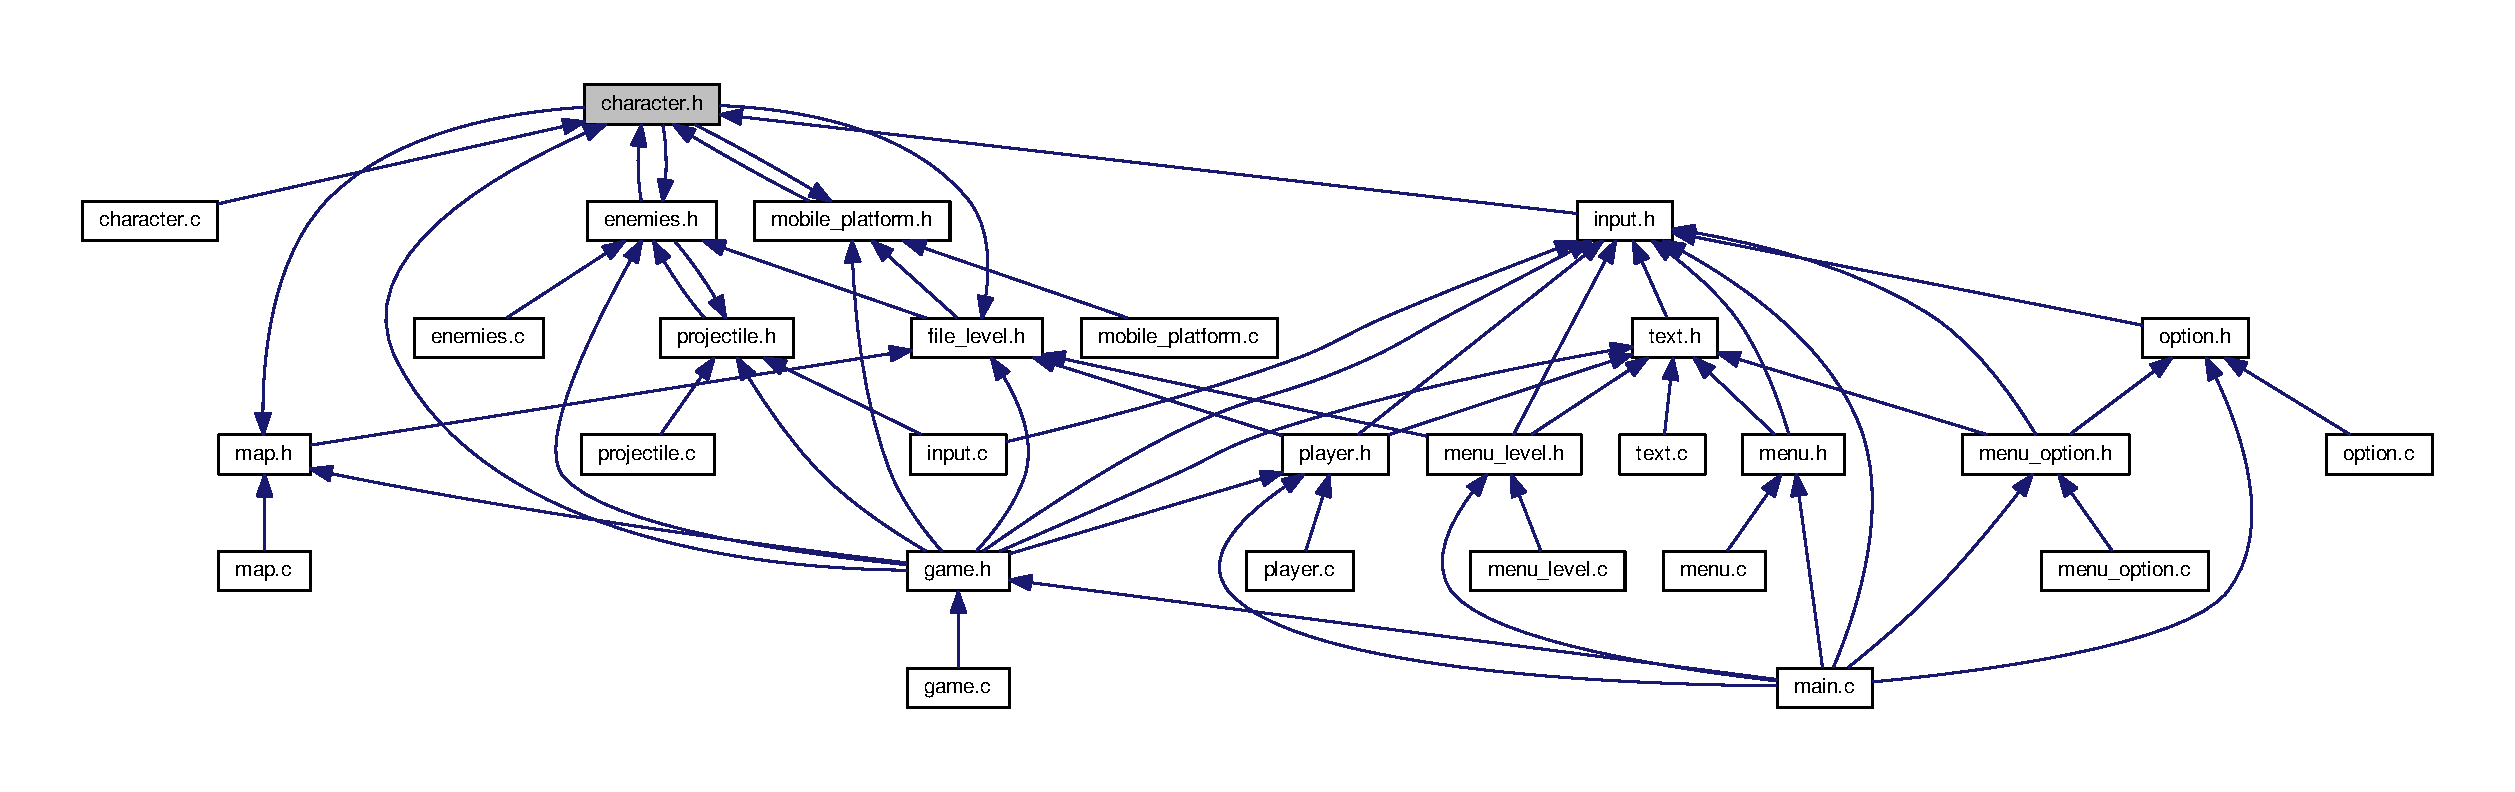
\includegraphics[width=350pt]{character_8h__dep__incl}
\end{center}
\end{figure}
\subsection*{Macros}
\begin{DoxyCompactItemize}
\item 
\#define \hyperlink{character_8h_a3af35b2f3ecf099e959f98d3aaa558a5}{S\-G\-N}(X)~(((X)==0)?(0)\-:(((X)$<$0)?(-\/1)\-:(1)))
\item 
\#define \hyperlink{character_8h_adefab4344518e9d35a80d87c20c0fa48}{A\-B\-S}(X)~((((X)$<$0)?(-\/(X))\-:(X)))
\end{DoxyCompactItemize}
\subsection*{Functions}
\begin{DoxyCompactItemize}
\item 
\hypertarget{character_8h_af96a38a849c14acb4b0e363493345442}{int {\bfseries move\-Character} (\hyperlink{struct_character}{Character} $\ast$c, float move\-\_\-left, float move\-\_\-right, int jump, \hyperlink{struct_map}{Map} $\ast$m, float $\ast$speed, \hyperlink{structlist}{list} $\ast$l, \hyperlink{struct_sound}{Sound} $\ast$s, \hyperlink{structplatform_set}{platform\-Set} $\ast$ps)}\label{character_8h_af96a38a849c14acb4b0e363493345442}

\item 
\hyperlink{struct_character}{Character} $\ast$ \hyperlink{character_8h_af17ad2fb50f637fe363a48e24727bbc0}{create\-Character} (char $\ast$tile, int x, int y, int npc, int nb\-Projectile, int nb\-Coins, int nb\-Lifes)
\item 
void \hyperlink{character_8h_a3c4b84a9d7123af243336f3540d2ae83}{blit\-Character} (S\-D\-L\-\_\-\-Surface $\ast$screen, \hyperlink{struct_character}{Character} $\ast$c, \hyperlink{struct_map}{Map} $\ast$m)
\item 
\hypertarget{character_8h_af15e182c04b17ce9a3d16872f2bf4f49}{int {\bfseries try\-Movement} (\hyperlink{struct_character}{Character} $\ast$c, int vx, int vy, \hyperlink{struct_map}{Map} $\ast$m, \hyperlink{structlist}{list} $\ast$l, \hyperlink{structplatform_set}{platform\-Set} $\ast$ps, \hyperlink{struct_sound}{Sound} $\ast$sound\-\_\-sys)}\label{character_8h_af15e182c04b17ce9a3d16872f2bf4f49}

\item 
\hypertarget{character_8h_a780616fe53145812a634dcf5e4f20959}{void {\bfseries presise\-Move\-Character} (\hyperlink{struct_character}{Character} $\ast$c, int vx, int vy, \hyperlink{struct_map}{Map} $\ast$m, \hyperlink{structlist}{list} $\ast$l, \hyperlink{structplatform_set}{platform\-Set} $\ast$ps)}\label{character_8h_a780616fe53145812a634dcf5e4f20959}

\item 
int \hyperlink{character_8h_a7b6d5ab652a57c5d6ffbaea628164402}{collision\-Sprite} (S\-D\-L\-\_\-\-Rect s1, S\-D\-L\-\_\-\-Rect s2)
\item 
int \hyperlink{character_8h_aea69b279f0dc778dde496ea610f1aa82}{check\-Fall} (\hyperlink{struct_character}{Character} $\ast$c, \hyperlink{struct_map}{Map} $\ast$m, \hyperlink{structplatform_set}{platform\-Set} $\ast$ps)
\item 
int \hyperlink{character_8h_a81dc963e2a308d0e3e627b7652aa7489}{check\-Wall} (\hyperlink{struct_character}{Character} $\ast$c, \hyperlink{struct_map}{Map} $\ast$m)
\end{DoxyCompactItemize}


\subsection{Detailed Description}
header de \hyperlink{character_8c}{character.\-c} \begin{DoxyAuthor}{Author}
Xavier C\-O\-P\-O\-N\-E\-T 
\end{DoxyAuthor}
\begin{DoxyDate}{Date}
2014-\/02-\/27 
\end{DoxyDate}


\subsection{Macro Definition Documentation}
\hypertarget{character_8h_adefab4344518e9d35a80d87c20c0fa48}{\index{character.\-h@{character.\-h}!A\-B\-S@{A\-B\-S}}
\index{A\-B\-S@{A\-B\-S}!character.h@{character.\-h}}
\subsubsection[{A\-B\-S}]{\setlength{\rightskip}{0pt plus 5cm}\#define A\-B\-S(
\begin{DoxyParamCaption}
\item[{}]{X}
\end{DoxyParamCaption}
)~((((X)$<$0)?(-\/(X))\-:(X)))}}\label{character_8h_adefab4344518e9d35a80d87c20c0fa48}
X absolute value \hypertarget{character_8h_a3af35b2f3ecf099e959f98d3aaa558a5}{\index{character.\-h@{character.\-h}!S\-G\-N@{S\-G\-N}}
\index{S\-G\-N@{S\-G\-N}!character.h@{character.\-h}}
\subsubsection[{S\-G\-N}]{\setlength{\rightskip}{0pt plus 5cm}\#define S\-G\-N(
\begin{DoxyParamCaption}
\item[{}]{X}
\end{DoxyParamCaption}
)~(((X)==0)?(0)\-:(((X)$<$0)?(-\/1)\-:(1)))}}\label{character_8h_a3af35b2f3ecf099e959f98d3aaa558a5}
X sign 

\subsection{Function Documentation}
\hypertarget{character_8h_a3c4b84a9d7123af243336f3540d2ae83}{\index{character.\-h@{character.\-h}!blit\-Character@{blit\-Character}}
\index{blit\-Character@{blit\-Character}!character.h@{character.\-h}}
\subsubsection[{blit\-Character}]{\setlength{\rightskip}{0pt plus 5cm}void blit\-Character (
\begin{DoxyParamCaption}
\item[{S\-D\-L\-\_\-\-Surface $\ast$}]{screen, }
\item[{{\bf Character} $\ast$}]{c, }
\item[{{\bf Map} $\ast$}]{m}
\end{DoxyParamCaption}
)}}\label{character_8h_a3c4b84a9d7123af243336f3540d2ae83}
blit the character 
\begin{DoxyParams}[1]{Parameters}
\mbox{\tt in,out}  & {\em screen} & game screen \\
\hline
\mbox{\tt in}  & {\em c} & the character \\
\hline
\mbox{\tt in}  & {\em m} & game map \\
\hline
\end{DoxyParams}
\hypertarget{character_8h_aea69b279f0dc778dde496ea610f1aa82}{\index{character.\-h@{character.\-h}!check\-Fall@{check\-Fall}}
\index{check\-Fall@{check\-Fall}!character.h@{character.\-h}}
\subsubsection[{check\-Fall}]{\setlength{\rightskip}{0pt plus 5cm}int check\-Fall (
\begin{DoxyParamCaption}
\item[{{\bf Character} $\ast$}]{c, }
\item[{{\bf Map} $\ast$}]{m, }
\item[{{\bf platform\-Set} $\ast$}]{ps}
\end{DoxyParamCaption}
)}}\label{character_8h_aea69b279f0dc778dde496ea610f1aa82}
tests if the character's futur position is over a void tile 
\begin{DoxyParams}[1]{Parameters}
\mbox{\tt in}  & {\em c} & the monster/character to be tested \\
\hline
\mbox{\tt in}  & {\em m} & the game map \\
\hline
\mbox{\tt in}  & {\em ps} & the platform set \\
\hline
\end{DoxyParams}
\begin{DoxyReturn}{Returns}
1 if void tile, 0 if not 
\end{DoxyReturn}
\hypertarget{character_8h_a81dc963e2a308d0e3e627b7652aa7489}{\index{character.\-h@{character.\-h}!check\-Wall@{check\-Wall}}
\index{check\-Wall@{check\-Wall}!character.h@{character.\-h}}
\subsubsection[{check\-Wall}]{\setlength{\rightskip}{0pt plus 5cm}int check\-Wall (
\begin{DoxyParamCaption}
\item[{{\bf Character} $\ast$}]{c, }
\item[{{\bf Map} $\ast$}]{m}
\end{DoxyParamCaption}
)}}\label{character_8h_a81dc963e2a308d0e3e627b7652aa7489}
tests if the character's futur position is next to a wall tile 
\begin{DoxyParams}[1]{Parameters}
\mbox{\tt in}  & {\em c} & the monster/character to be tested \\
\hline
\mbox{\tt in}  & {\em m} & the game map \\
\hline
\end{DoxyParams}
\begin{DoxyReturn}{Returns}
1 if wall tile, 0 if not 
\end{DoxyReturn}
\hypertarget{character_8h_a7b6d5ab652a57c5d6ffbaea628164402}{\index{character.\-h@{character.\-h}!collision\-Sprite@{collision\-Sprite}}
\index{collision\-Sprite@{collision\-Sprite}!character.h@{character.\-h}}
\subsubsection[{collision\-Sprite}]{\setlength{\rightskip}{0pt plus 5cm}int collision\-Sprite (
\begin{DoxyParamCaption}
\item[{S\-D\-L\-\_\-\-Rect}]{s1, }
\item[{S\-D\-L\-\_\-\-Rect}]{s2}
\end{DoxyParamCaption}
)}}\label{character_8h_a7b6d5ab652a57c5d6ffbaea628164402}
int \hyperlink{character_8h_a7b6d5ab652a57c5d6ffbaea628164402}{collision\-Sprite(\-S\-D\-L\-\_\-\-Rect s1, S\-D\-L\-\_\-\-Rect s2)} determine if there is a collision beteewen two sprites 
\begin{DoxyParams}[1]{Parameters}
\mbox{\tt in}  & {\em s1} & the first sprite \\
\hline
\mbox{\tt in}  & {\em s2} & the second sprite \\
\hline
\end{DoxyParams}
\begin{DoxyReturn}{Returns}
3 if there is a collision and s1 is below s2, 2 if there is a collision and s1 is over s2, 0 if there is no collision 
\end{DoxyReturn}
\hypertarget{character_8h_af17ad2fb50f637fe363a48e24727bbc0}{\index{character.\-h@{character.\-h}!create\-Character@{create\-Character}}
\index{create\-Character@{create\-Character}!character.h@{character.\-h}}
\subsubsection[{create\-Character}]{\setlength{\rightskip}{0pt plus 5cm}{\bf Character}$\ast$ create\-Character (
\begin{DoxyParamCaption}
\item[{char $\ast$}]{tile, }
\item[{int}]{x, }
\item[{int}]{y, }
\item[{int}]{npc, }
\item[{int}]{nb\-Projectile, }
\item[{int}]{nb\-Coins, }
\item[{int}]{nb\-Lifes}
\end{DoxyParamCaption}
)}}\label{character_8h_af17ad2fb50f637fe363a48e24727bbc0}
create a character 
\begin{DoxyParams}[1]{Parameters}
\mbox{\tt in}  & {\em tile} & character tile\-Set address \\
\hline
\mbox{\tt in}  & {\em x} & character's x location \\
\hline
\mbox{\tt in}  & {\em y} & character's y location \\
\hline
\mbox{\tt in}  & {\em npc} & type of npc if creating a npc, 0 if not \\
\hline
\mbox{\tt in}  & {\em nb\-Projectile} & the number of projectiles the character has \\
\hline
\mbox{\tt in}  & {\em nb\-Coins} & the number of coins the character has \\
\hline
\mbox{\tt in}  & {\em nb\-Lifes} & the number of life the character has \\
\hline
\end{DoxyParams}
\begin{DoxyReturn}{Returns}
character structure pointer 
\end{DoxyReturn}


Here is the call graph for this function\-:
\nopagebreak
\begin{figure}[H]
\begin{center}
\leavevmode
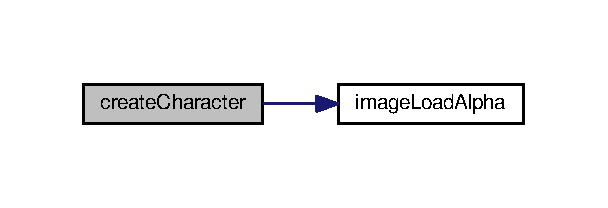
\includegraphics[width=292pt]{character_8h_af17ad2fb50f637fe363a48e24727bbc0_cgraph}
\end{center}
\end{figure}



\hypertarget{const_8h}{\section{const.\-h File Reference}
\label{const_8h}\index{const.\-h@{const.\-h}}
}


contient les constantes du programme  


This graph shows which files directly or indirectly include this file\-:\nopagebreak
\begin{figure}[H]
\begin{center}
\leavevmode
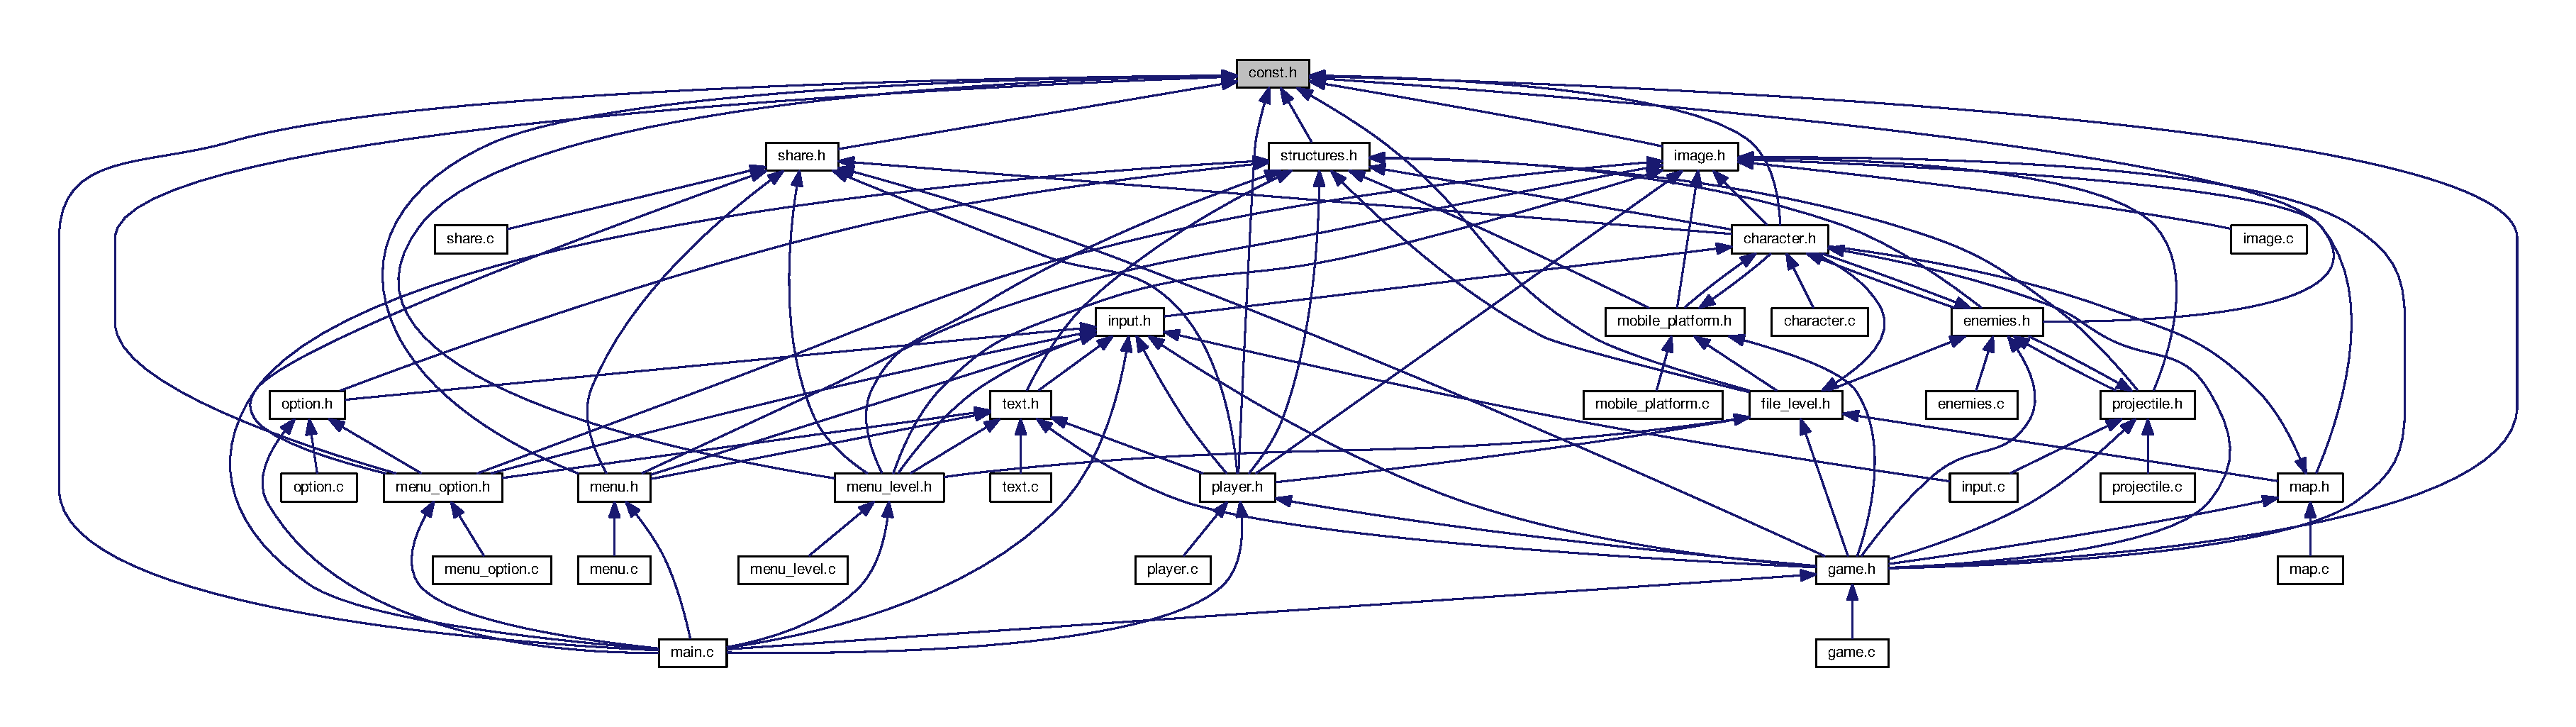
\includegraphics[width=350pt]{const_8h__dep__incl}
\end{center}
\end{figure}
\subsection*{Data Structures}
\begin{DoxyCompactItemize}
\item 
struct \hyperlink{struct_level}{Level}
\item 
struct \hyperlink{struct_map}{Map}
\end{DoxyCompactItemize}
\subsection*{Macros}
\begin{DoxyCompactItemize}
\item 
\hypertarget{const_8h_abad9ad5ae94fd56569e71c156349030b}{\#define {\bfseries T\-A\-I\-L\-L\-E\-\_\-\-B\-L\-O\-C}~16}\label{const_8h_abad9ad5ae94fd56569e71c156349030b}

\item 
\hypertarget{const_8h_a5b621c07985e98b04fc2d2195b85ad69}{\#define {\bfseries N\-B\-\_\-\-B\-L\-O\-C\-S\-\_\-\-L\-A\-R\-G\-E\-U\-R}~60}\label{const_8h_a5b621c07985e98b04fc2d2195b85ad69}

\item 
\hypertarget{const_8h_ad0de8de53b10369f89648fed34ce16c9}{\#define {\bfseries N\-B\-\_\-\-B\-L\-O\-C\-S\-\_\-\-H\-A\-U\-T\-E\-U\-R}~33}\label{const_8h_ad0de8de53b10369f89648fed34ce16c9}

\item 
\hypertarget{const_8h_a6068a247ff9ece1b0a9773c58144906c}{\#define {\bfseries L\-A\-R\-G\-E\-U\-R\-\_\-\-F\-E\-N\-E\-T\-R\-E}~T\-A\-I\-L\-L\-E\-\_\-\-B\-L\-O\-C $\ast$ N\-B\-\_\-\-B\-L\-O\-C\-S\-\_\-\-L\-A\-R\-G\-E\-U\-R}\label{const_8h_a6068a247ff9ece1b0a9773c58144906c}

\item 
\hypertarget{const_8h_afd1a1e285af564b849b17498e82e1a41}{\#define {\bfseries H\-A\-U\-T\-E\-U\-R\-\_\-\-F\-E\-N\-E\-T\-R\-E}~T\-A\-I\-L\-L\-E\-\_\-\-B\-L\-O\-C $\ast$ N\-B\-\_\-\-B\-L\-O\-C\-S\-\_\-\-H\-A\-U\-T\-E\-U\-R}\label{const_8h_afd1a1e285af564b849b17498e82e1a41}

\item 
\hypertarget{const_8h_ac92ca5ab87034a348decad7ee8d4bd1b}{\#define {\bfseries F\-P\-S}~60}\label{const_8h_ac92ca5ab87034a348decad7ee8d4bd1b}

\item 
\hypertarget{const_8h_a26141a4793db30295b597c3af901ddc8}{\#define {\bfseries T\-A\-I\-L\-L\-E\-\_\-\-M\-A\-X\-\_\-\-N\-O\-M\-\_\-\-F\-I\-C\-H\-I\-E\-R}~100}\label{const_8h_a26141a4793db30295b597c3af901ddc8}

\item 
\hypertarget{const_8h_a4295bab46a8fdcf8ff2106b2c32f15ad}{\#define {\bfseries T\-A\-I\-L\-L\-E\-\_\-\-S\-A\-U\-T}~17}\label{const_8h_a4295bab46a8fdcf8ff2106b2c32f15ad}

\item 
\hypertarget{const_8h_afe523953f60b9d8b73d97c8c673ef884}{\#define {\bfseries M\-A\-R\-G\-E\-\_\-\-S\-C\-R\-O\-L\-L\-I\-N\-G}~2}\label{const_8h_afe523953f60b9d8b73d97c8c673ef884}

\item 
\hypertarget{const_8h_a848d259eb2345aaa73fdfaeffb59afbd}{\#define {\bfseries P\-O\-U\-R\-C\-E\-N\-T\-A\-G\-E\-\_\-\-D\-E\-P\-L\-A\-C\-E\-M\-E\-N\-T}~0}\label{const_8h_a848d259eb2345aaa73fdfaeffb59afbd}

\item 
\hypertarget{const_8h_a95addb9496c5772d6e7bc43eabb16d8b}{\#define {\bfseries T\-I\-L\-E\-\_\-\-M\-A\-X}~8}\label{const_8h_a95addb9496c5772d6e7bc43eabb16d8b}

\end{DoxyCompactItemize}
\subsection*{Enumerations}
\begin{DoxyCompactItemize}
\item 
enum \{ {\bfseries V\-O\-I\-D} =0, 
{\bfseries G\-R\-A\-S\-S1} =1, 
{\bfseries G\-R\-O\-U\-N\-D1} =2, 
{\bfseries G\-R\-E\-Y\-\_\-\-W\-A\-L\-L} =3
 \}
\item 
enum \{ {\bfseries R\-I\-G\-H\-T}, 
{\bfseries L\-E\-F\-T}, 
{\bfseries U\-P}, 
{\bfseries D\-O\-W\-N}
 \}
\end{DoxyCompactItemize}


\subsection{Detailed Description}
contient les constantes du programme \begin{DoxyAuthor}{Author}
Xavier C\-O\-P\-O\-N\-E\-T 
\end{DoxyAuthor}
\begin{DoxyDate}{Date}
2014-\/02-\/27 
\end{DoxyDate}

\hypertarget{enemies_8c}{\section{enemies.\-c File Reference}
\label{enemies_8c}\index{enemies.\-c@{enemies.\-c}}
}


contain enemies gestion function  


{\ttfamily \#include \char`\"{}enemies.\-h\char`\"{}}\\*
Include dependency graph for enemies.\-c\-:
\nopagebreak
\begin{figure}[H]
\begin{center}
\leavevmode
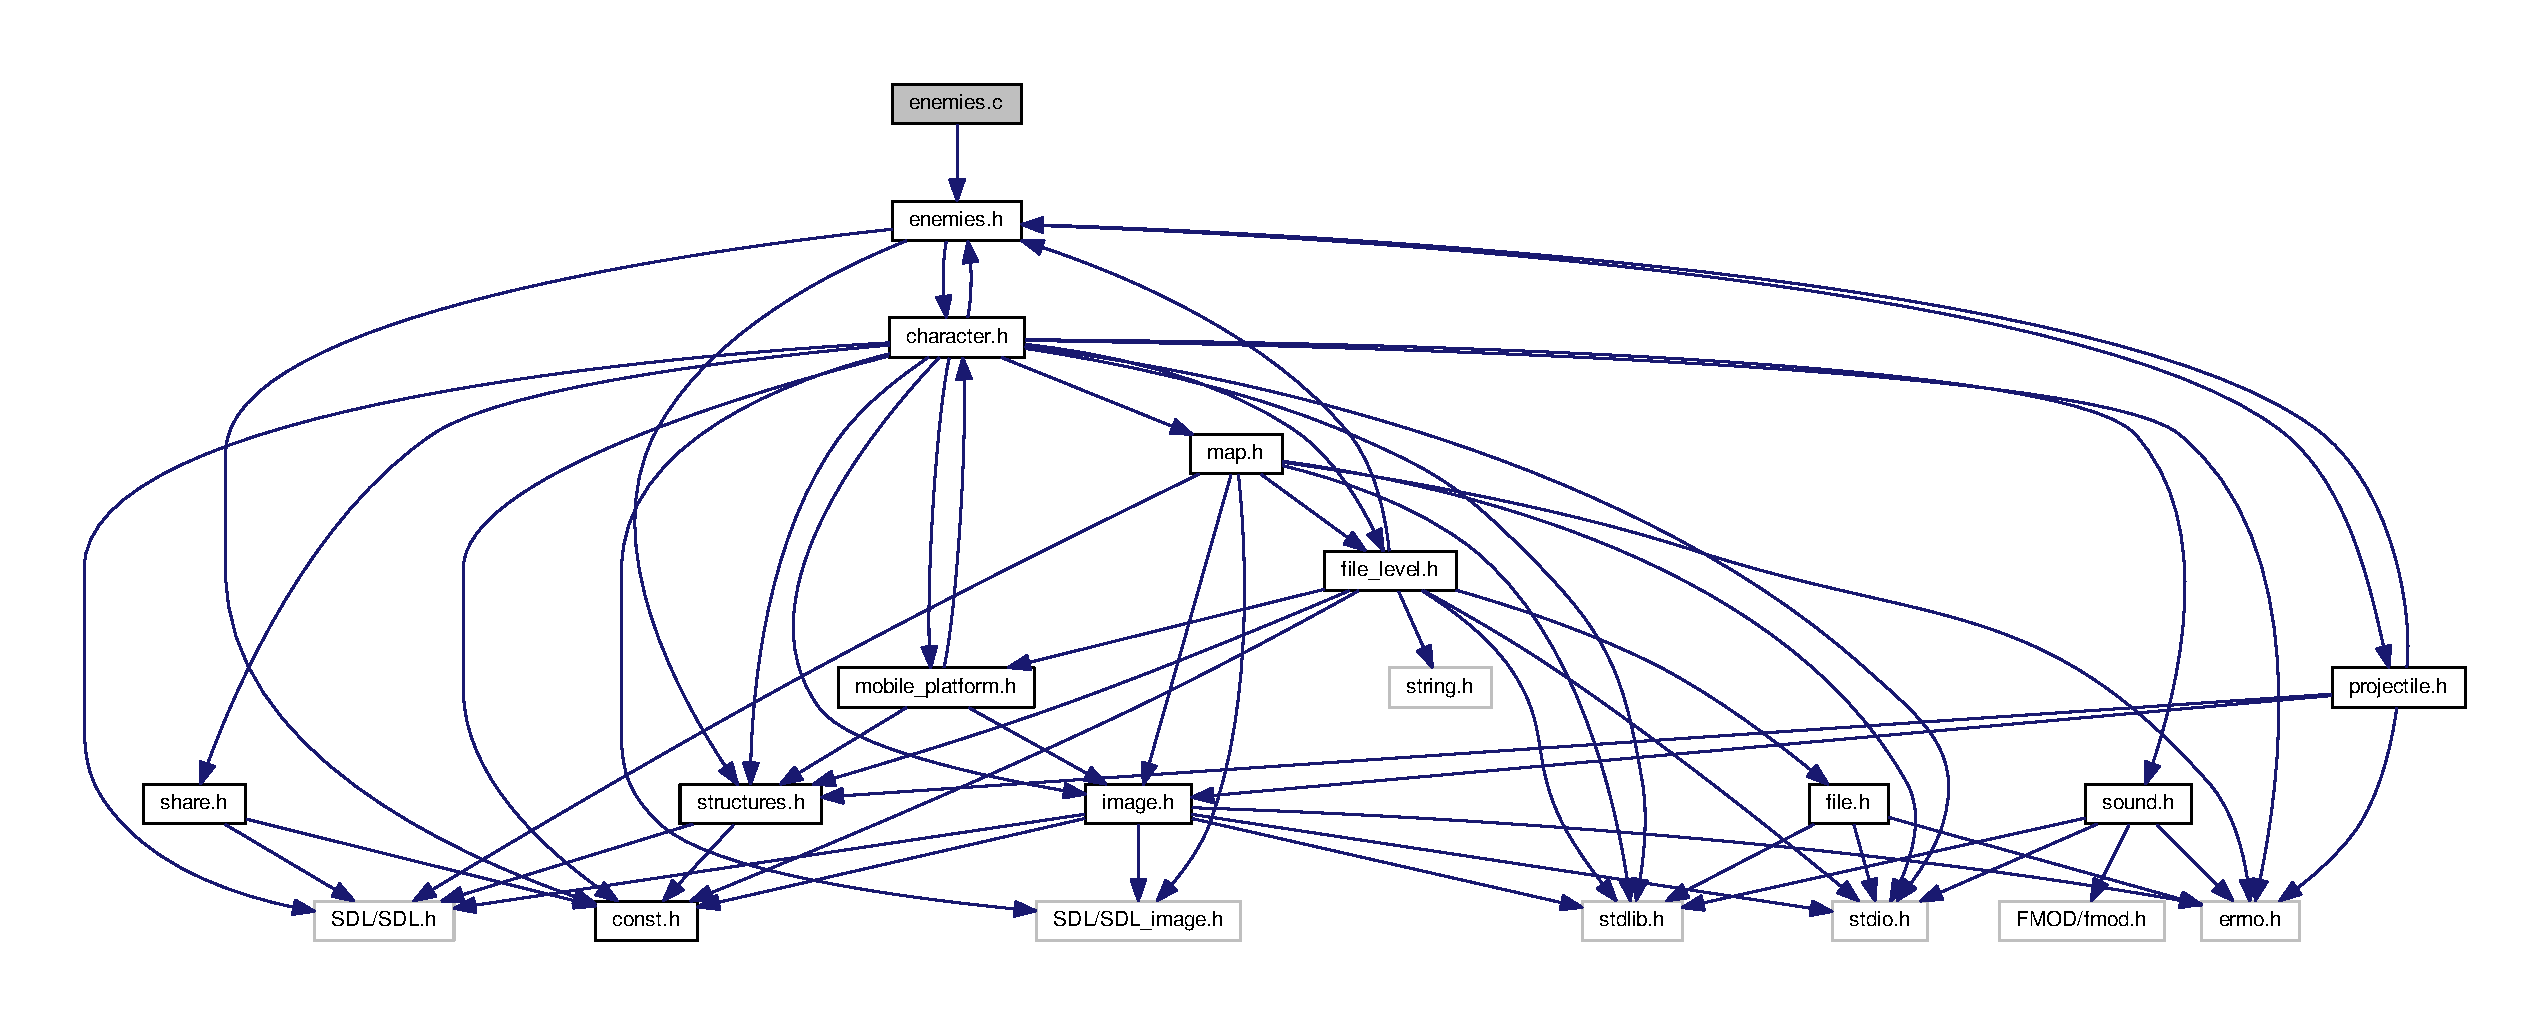
\includegraphics[width=350pt]{enemies_8c__incl}
\end{center}
\end{figure}
\subsection*{Functions}
\begin{DoxyCompactItemize}
\item 
\hypertarget{enemies_8c_a68e86bc615a3b71cf549b32a71f6c943}{void {\bfseries create\-Enemy} (char $\ast$tile, int x, int y, \hyperlink{structlist}{list} $\ast$l, int type)}\label{enemies_8c_a68e86bc615a3b71cf549b32a71f6c943}

\item 
void \hyperlink{enemies_8c_a766e049c933ace6a69ba1e7c3fab142c}{free\-Enemies} (\hyperlink{structlist}{list} $\ast$l)
\item 
\hypertarget{enemies_8c_ada7bfd5ddcfd60cd52ad17b2c9b37b8f}{void {\bfseries blit\-Enemies} (S\-D\-L\-\_\-\-Surface $\ast$screen, \hyperlink{structlist}{list} $\ast$l, \hyperlink{struct_map}{Map} $\ast$m)}\label{enemies_8c_ada7bfd5ddcfd60cd52ad17b2c9b37b8f}

\item 
int \hyperlink{enemies_8c_ae36bc711341ade0e08eb57e1c5063174}{collision\-Enemy} (\hyperlink{struct_character}{Character} $\ast$c, \hyperlink{structlist}{list} $\ast$l, \hyperlink{struct_map}{Map} $\ast$m)
\item 
\hypertarget{enemies_8c_a5cc0822e34be00f2555f70f8acf17680}{void {\bfseries move\-Enemies} (\hyperlink{structlist}{list} $\ast$l, \hyperlink{struct_map}{Map} $\ast$m, \hyperlink{structlist}{list} $\ast$p, \hyperlink{structprojectile_set}{projectile\-Set} $\ast$ps, int $\ast$launch)}\label{enemies_8c_a5cc0822e34be00f2555f70f8acf17680}

\item 
\hypertarget{enemies_8c_a315db1acddbe1cd18db63bab85f1709a}{int {\bfseries move\-Character\-Col} (\hyperlink{struct_character}{Character} $\ast$c, int move\-\_\-left, int move\-\_\-right, \hyperlink{struct_map}{Map} $\ast$m)}\label{enemies_8c_a315db1acddbe1cd18db63bab85f1709a}

\item 
\hypertarget{enemies_8c_a86da34107b65b23bb7105568af701160}{\hyperlink{structnode}{node} $\ast$ {\bfseries new\-Node} (\hyperlink{struct_character}{Character} $\ast$c, \hyperlink{structnode}{node} $\ast$n, \hyperlink{structnode}{node} $\ast$p)}\label{enemies_8c_a86da34107b65b23bb7105568af701160}

\item 
void \hyperlink{enemies_8c_aaca0e3ca99177d70268a1f770c50e264}{init\-List} (\hyperlink{structlist}{list} $\ast$l)
\item 
int \hyperlink{enemies_8c_a185b7dd5b77fdf2b6315358ac7767e44}{empty} (\hyperlink{structlist}{list} $\ast$l)
\item 
int \hyperlink{enemies_8c_a0f5c139f75d0a54b38c0d33e1bc22223}{first} (\hyperlink{structlist}{list} $\ast$l)
\item 
int \hyperlink{enemies_8c_a86d339159e440962ce42347b99e07625}{last} (\hyperlink{structlist}{list} $\ast$l)
\item 
int \hyperlink{enemies_8c_a7774be61944dce2ae021e0e4442b4515}{out\-Of\-List} (\hyperlink{structlist}{list} $\ast$l)
\item 
void \hyperlink{enemies_8c_aa0ae9a01476366cb08c3e904e2f31433}{set\-On\-First} (\hyperlink{structlist}{list} $\ast$l)
\item 
void \hyperlink{enemies_8c_ad8a2ca1098f3a37401100bf88c3a4f03}{set\-On\-Last} (\hyperlink{structlist}{list} $\ast$l)
\item 
void \hyperlink{enemies_8c_a1e9424bcb6302d001589f04a99802abf}{next} (\hyperlink{structlist}{list} $\ast$l)
\item 
void \hyperlink{enemies_8c_ab6a55e4b951590640debd7d4110c37e6}{previous} (\hyperlink{structlist}{list} $\ast$l)
\item 
\hyperlink{struct_character}{Character} $\ast$ \hyperlink{enemies_8c_ad2b7dfcca2dece6a5c7deffdf0b6a4b1}{get\-Current} (\hyperlink{structlist}{list} $\ast$l)
\item 
\hypertarget{enemies_8c_a277ce428e10c4d50abdae6d162128f48}{int {\bfseries insert\-First} (\hyperlink{structlist}{list} $\ast$l, \hyperlink{struct_character}{Character} $\ast$c)}\label{enemies_8c_a277ce428e10c4d50abdae6d162128f48}

\item 
\hypertarget{enemies_8c_a121944b1f370af47e1f980128bf0fc86}{int {\bfseries insert\-Last} (\hyperlink{structlist}{list} $\ast$l, \hyperlink{struct_character}{Character} $\ast$c)}\label{enemies_8c_a121944b1f370af47e1f980128bf0fc86}

\item 
\hypertarget{enemies_8c_ae745be19268624b512665dce384c7eb4}{int {\bfseries insert\-After\-Current} (\hyperlink{structlist}{list} $\ast$l, \hyperlink{struct_character}{Character} $\ast$c)}\label{enemies_8c_ae745be19268624b512665dce384c7eb4}

\item 
\hypertarget{enemies_8c_ae8c5bac4a4363592b055b0cd4000864c}{int {\bfseries insert\-Before\-Current} (\hyperlink{structlist}{list} $\ast$l, \hyperlink{struct_character}{Character} $\ast$c)}\label{enemies_8c_ae8c5bac4a4363592b055b0cd4000864c}

\item 
\hyperlink{struct_character}{Character} $\ast$ \hyperlink{enemies_8c_a1d19853ad1ad5712c72159157e026164}{delete\-First} (\hyperlink{structlist}{list} $\ast$l)
\item 
\hyperlink{struct_character}{Character} $\ast$ \hyperlink{enemies_8c_ae74eb855c1a8951c927e7322c08b33c0}{delete\-Last} (\hyperlink{structlist}{list} $\ast$l)
\item 
\hyperlink{struct_character}{Character} $\ast$ \hyperlink{enemies_8c_afd06d60d09ccb8510aa7e8fe1246094b}{delete\-Current} (\hyperlink{structlist}{list} $\ast$l)
\end{DoxyCompactItemize}


\subsection{Detailed Description}
contain enemies gestion function \begin{DoxyAuthor}{Author}
Xavier C\-O\-P\-O\-N\-E\-T 
\end{DoxyAuthor}
\begin{DoxyDate}{Date}
2014-\/04-\/14 
\end{DoxyDate}


\subsection{Function Documentation}
\hypertarget{enemies_8c_ae36bc711341ade0e08eb57e1c5063174}{\index{enemies.\-c@{enemies.\-c}!collision\-Enemy@{collision\-Enemy}}
\index{collision\-Enemy@{collision\-Enemy}!enemies.c@{enemies.\-c}}
\subsubsection[{collision\-Enemy}]{\setlength{\rightskip}{0pt plus 5cm}int collision\-Enemy (
\begin{DoxyParamCaption}
\item[{{\bf Character} $\ast$}]{c, }
\item[{{\bf list} $\ast$}]{l, }
\item[{{\bf Map} $\ast$}]{m}
\end{DoxyParamCaption}
)}}\label{enemies_8c_ae36bc711341ade0e08eb57e1c5063174}
determine if there is a collision beteewen the player sprite and an enemy and deals with 
\begin{DoxyParams}[1]{Parameters}
\mbox{\tt in,out}  & {\em c} & the player \\
\hline
\mbox{\tt in,out}  & {\em l} & the enemy list, change the current node \\
\hline
\mbox{\tt in}  & {\em m} & the game map \\
\hline
\end{DoxyParams}
\begin{DoxyReturn}{Returns}
1 if there is a collision, 0 if not 
\end{DoxyReturn}


Here is the call graph for this function\-:
\nopagebreak
\begin{figure}[H]
\begin{center}
\leavevmode
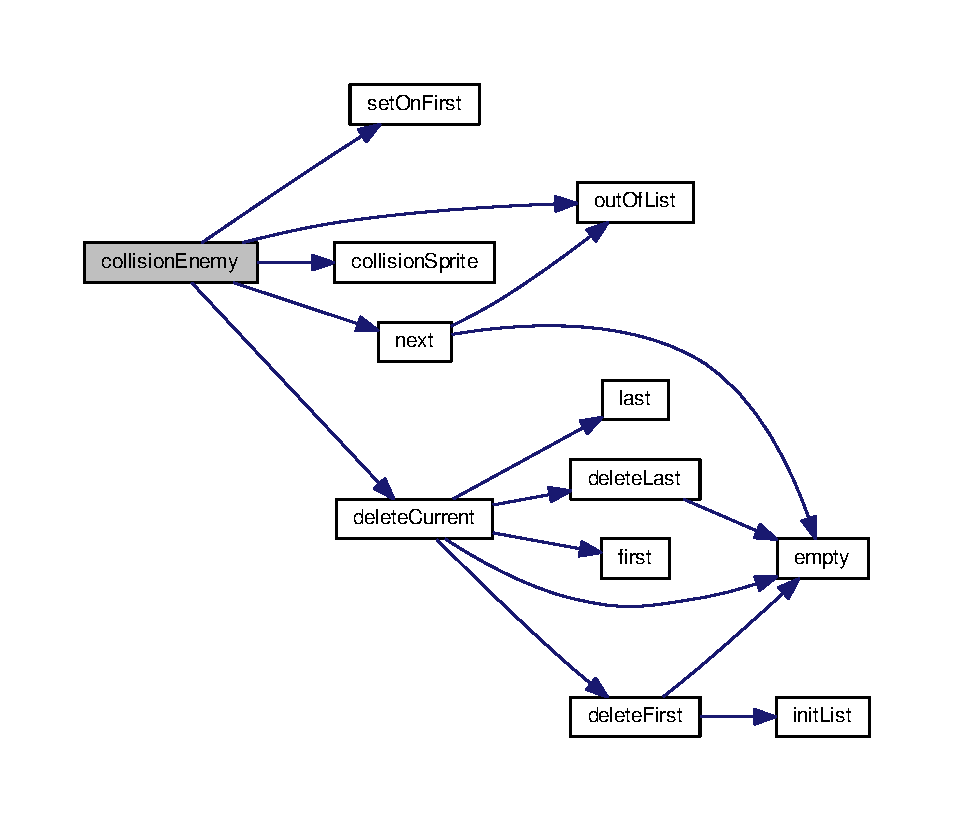
\includegraphics[width=350pt]{enemies_8c_ae36bc711341ade0e08eb57e1c5063174_cgraph}
\end{center}
\end{figure}


\hypertarget{enemies_8c_afd06d60d09ccb8510aa7e8fe1246094b}{\index{enemies.\-c@{enemies.\-c}!delete\-Current@{delete\-Current}}
\index{delete\-Current@{delete\-Current}!enemies.c@{enemies.\-c}}
\subsubsection[{delete\-Current}]{\setlength{\rightskip}{0pt plus 5cm}enemy $\ast$ delete\-Current (
\begin{DoxyParamCaption}
\item[{{\bf list} $\ast$}]{l}
\end{DoxyParamCaption}
)}}\label{enemies_8c_afd06d60d09ccb8510aa7e8fe1246094b}
delete the current node 
\begin{DoxyParams}[1]{Parameters}
\mbox{\tt out}  & {\em l} & the list which has to be modified \\
\hline
\end{DoxyParams}
\begin{DoxyReturn}{Returns}
the current node's enemy, N\-U\-L\-L if empty list 
\end{DoxyReturn}


Here is the call graph for this function\-:
\nopagebreak
\begin{figure}[H]
\begin{center}
\leavevmode
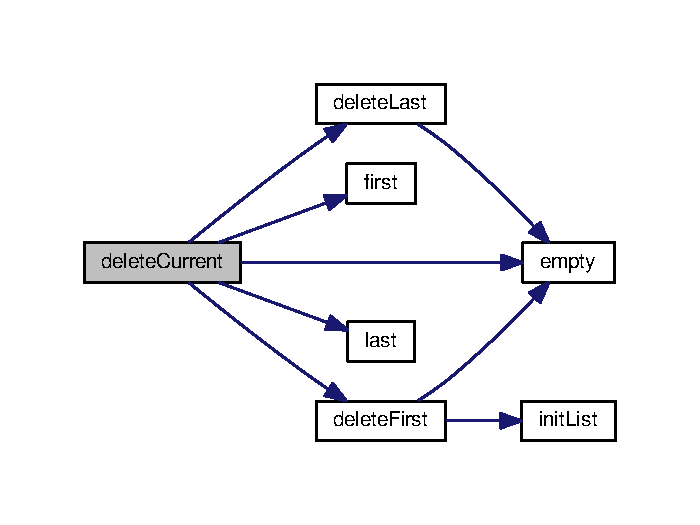
\includegraphics[width=336pt]{enemies_8c_afd06d60d09ccb8510aa7e8fe1246094b_cgraph}
\end{center}
\end{figure}


\hypertarget{enemies_8c_a1d19853ad1ad5712c72159157e026164}{\index{enemies.\-c@{enemies.\-c}!delete\-First@{delete\-First}}
\index{delete\-First@{delete\-First}!enemies.c@{enemies.\-c}}
\subsubsection[{delete\-First}]{\setlength{\rightskip}{0pt plus 5cm}enemy $\ast$ delete\-First (
\begin{DoxyParamCaption}
\item[{{\bf list} $\ast$}]{l}
\end{DoxyParamCaption}
)}}\label{enemies_8c_a1d19853ad1ad5712c72159157e026164}
delete the first node 
\begin{DoxyParams}[1]{Parameters}
\mbox{\tt out}  & {\em l} & the list which has to be modified \\
\hline
\end{DoxyParams}
\begin{DoxyReturn}{Returns}
the first node's enemy, N\-U\-L\-L if empty list 
\end{DoxyReturn}


Here is the call graph for this function\-:
\nopagebreak
\begin{figure}[H]
\begin{center}
\leavevmode
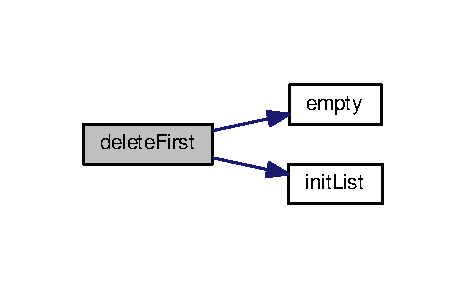
\includegraphics[width=224pt]{enemies_8c_a1d19853ad1ad5712c72159157e026164_cgraph}
\end{center}
\end{figure}


\hypertarget{enemies_8c_ae74eb855c1a8951c927e7322c08b33c0}{\index{enemies.\-c@{enemies.\-c}!delete\-Last@{delete\-Last}}
\index{delete\-Last@{delete\-Last}!enemies.c@{enemies.\-c}}
\subsubsection[{delete\-Last}]{\setlength{\rightskip}{0pt plus 5cm}enemy $\ast$ delete\-Last (
\begin{DoxyParamCaption}
\item[{{\bf list} $\ast$}]{l}
\end{DoxyParamCaption}
)}}\label{enemies_8c_ae74eb855c1a8951c927e7322c08b33c0}
delete the last node 
\begin{DoxyParams}[1]{Parameters}
\mbox{\tt out}  & {\em l} & the list which has to be modified \\
\hline
\end{DoxyParams}
\begin{DoxyReturn}{Returns}
the last node's enemy, N\-U\-L\-L if empty list 
\end{DoxyReturn}


Here is the call graph for this function\-:
\nopagebreak
\begin{figure}[H]
\begin{center}
\leavevmode
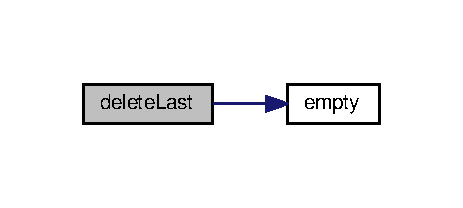
\includegraphics[width=222pt]{enemies_8c_ae74eb855c1a8951c927e7322c08b33c0_cgraph}
\end{center}
\end{figure}


\hypertarget{enemies_8c_a185b7dd5b77fdf2b6315358ac7767e44}{\index{enemies.\-c@{enemies.\-c}!empty@{empty}}
\index{empty@{empty}!enemies.c@{enemies.\-c}}
\subsubsection[{empty}]{\setlength{\rightskip}{0pt plus 5cm}int empty (
\begin{DoxyParamCaption}
\item[{{\bf list} $\ast$}]{l}
\end{DoxyParamCaption}
)}}\label{enemies_8c_a185b7dd5b77fdf2b6315358ac7767e44}
tests if the list is empty 
\begin{DoxyParams}[1]{Parameters}
\mbox{\tt in}  & {\em l} & the list to be tested \\
\hline
\end{DoxyParams}
\begin{DoxyReturn}{Returns}
1 if the list is empty, 0 if not 
\end{DoxyReturn}
\hypertarget{enemies_8c_a0f5c139f75d0a54b38c0d33e1bc22223}{\index{enemies.\-c@{enemies.\-c}!first@{first}}
\index{first@{first}!enemies.c@{enemies.\-c}}
\subsubsection[{first}]{\setlength{\rightskip}{0pt plus 5cm}int first (
\begin{DoxyParamCaption}
\item[{{\bf list} $\ast$}]{l}
\end{DoxyParamCaption}
)}}\label{enemies_8c_a0f5c139f75d0a54b38c0d33e1bc22223}
tests if the current node is the first node 
\begin{DoxyParams}[1]{Parameters}
\mbox{\tt in}  & {\em l} & the list to be tested \\
\hline
\end{DoxyParams}
\begin{DoxyReturn}{Returns}
1 if the current node is the first node, 0 if not 
\end{DoxyReturn}
\hypertarget{enemies_8c_a766e049c933ace6a69ba1e7c3fab142c}{\index{enemies.\-c@{enemies.\-c}!free\-Enemies@{free\-Enemies}}
\index{free\-Enemies@{free\-Enemies}!enemies.c@{enemies.\-c}}
\subsubsection[{free\-Enemies}]{\setlength{\rightskip}{0pt plus 5cm}void free\-Enemies (
\begin{DoxyParamCaption}
\item[{{\bf list} $\ast$}]{l}
\end{DoxyParamCaption}
)}}\label{enemies_8c_a766e049c933ace6a69ba1e7c3fab142c}
free all the enemies and the list 
\begin{DoxyParams}[1]{Parameters}
\mbox{\tt out}  & {\em l} & the enemy list \\
\hline
\end{DoxyParams}


Here is the call graph for this function\-:
\nopagebreak
\begin{figure}[H]
\begin{center}
\leavevmode
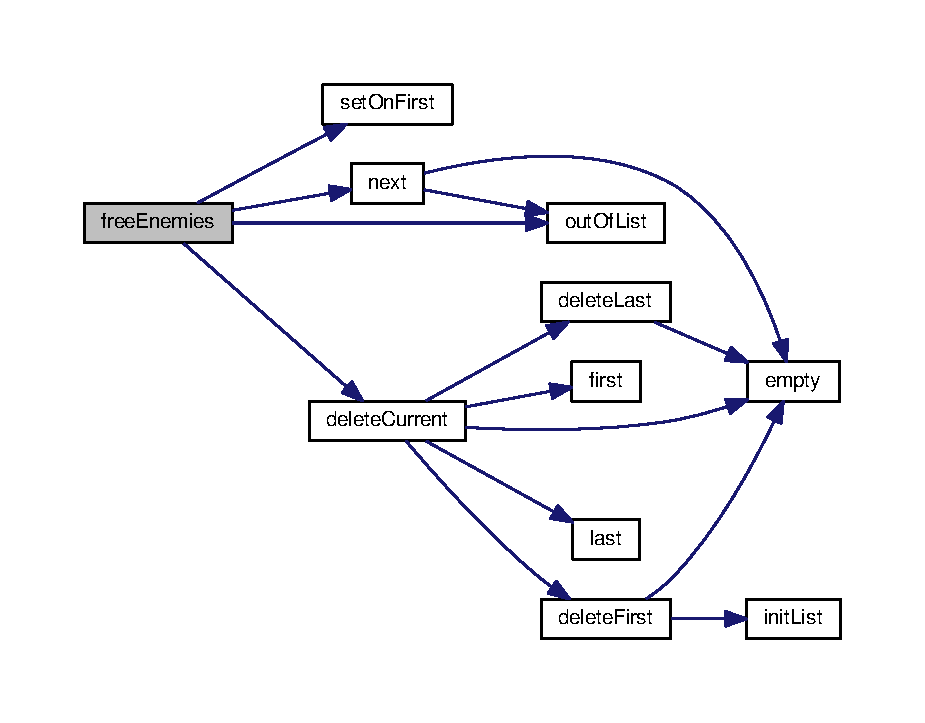
\includegraphics[width=350pt]{enemies_8c_a766e049c933ace6a69ba1e7c3fab142c_cgraph}
\end{center}
\end{figure}


\hypertarget{enemies_8c_ad2b7dfcca2dece6a5c7deffdf0b6a4b1}{\index{enemies.\-c@{enemies.\-c}!get\-Current@{get\-Current}}
\index{get\-Current@{get\-Current}!enemies.c@{enemies.\-c}}
\subsubsection[{get\-Current}]{\setlength{\rightskip}{0pt plus 5cm}enemy $\ast$ get\-Current (
\begin{DoxyParamCaption}
\item[{{\bf list} $\ast$}]{l}
\end{DoxyParamCaption}
)}}\label{enemies_8c_ad2b7dfcca2dece6a5c7deffdf0b6a4b1}
get the character of the current node 
\begin{DoxyParams}[1]{Parameters}
\mbox{\tt in}  & {\em l} & the list to be modified \\
\hline
\end{DoxyParams}
\hypertarget{enemies_8c_aaca0e3ca99177d70268a1f770c50e264}{\index{enemies.\-c@{enemies.\-c}!init\-List@{init\-List}}
\index{init\-List@{init\-List}!enemies.c@{enemies.\-c}}
\subsubsection[{init\-List}]{\setlength{\rightskip}{0pt plus 5cm}void init\-List (
\begin{DoxyParamCaption}
\item[{{\bf list} $\ast$}]{l}
\end{DoxyParamCaption}
)}}\label{enemies_8c_aaca0e3ca99177d70268a1f770c50e264}
initialize the enemy list 
\begin{DoxyParams}[1]{Parameters}
\mbox{\tt out}  & {\em l} & the list to be initalized \\
\hline
\end{DoxyParams}
\hypertarget{enemies_8c_a86d339159e440962ce42347b99e07625}{\index{enemies.\-c@{enemies.\-c}!last@{last}}
\index{last@{last}!enemies.c@{enemies.\-c}}
\subsubsection[{last}]{\setlength{\rightskip}{0pt plus 5cm}int last (
\begin{DoxyParamCaption}
\item[{{\bf list} $\ast$}]{l}
\end{DoxyParamCaption}
)}}\label{enemies_8c_a86d339159e440962ce42347b99e07625}
tests if the current node is the last node 
\begin{DoxyParams}[1]{Parameters}
\mbox{\tt in}  & {\em l} & the list to be tested \\
\hline
\end{DoxyParams}
\begin{DoxyReturn}{Returns}
1 if the current node is the last node, 0 if not 
\end{DoxyReturn}
\hypertarget{enemies_8c_a1e9424bcb6302d001589f04a99802abf}{\index{enemies.\-c@{enemies.\-c}!next@{next}}
\index{next@{next}!enemies.c@{enemies.\-c}}
\subsubsection[{next}]{\setlength{\rightskip}{0pt plus 5cm}void next (
\begin{DoxyParamCaption}
\item[{{\bf list} $\ast$}]{l}
\end{DoxyParamCaption}
)}}\label{enemies_8c_a1e9424bcb6302d001589f04a99802abf}
set the current node on its next node 
\begin{DoxyParams}[1]{Parameters}
\mbox{\tt out}  & {\em l} & the list to be modified \\
\hline
\end{DoxyParams}


Here is the call graph for this function\-:
\nopagebreak
\begin{figure}[H]
\begin{center}
\leavevmode
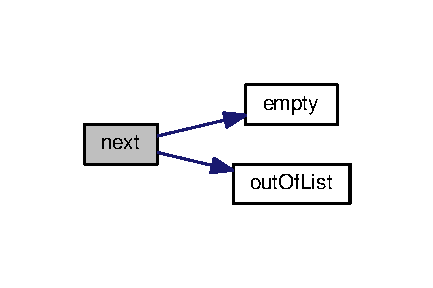
\includegraphics[width=208pt]{enemies_8c_a1e9424bcb6302d001589f04a99802abf_cgraph}
\end{center}
\end{figure}


\hypertarget{enemies_8c_a7774be61944dce2ae021e0e4442b4515}{\index{enemies.\-c@{enemies.\-c}!out\-Of\-List@{out\-Of\-List}}
\index{out\-Of\-List@{out\-Of\-List}!enemies.c@{enemies.\-c}}
\subsubsection[{out\-Of\-List}]{\setlength{\rightskip}{0pt plus 5cm}int out\-Of\-List (
\begin{DoxyParamCaption}
\item[{{\bf list} $\ast$}]{l}
\end{DoxyParamCaption}
)}}\label{enemies_8c_a7774be61944dce2ae021e0e4442b4515}
tests if the current node is in the list 
\begin{DoxyParams}[1]{Parameters}
\mbox{\tt in}  & {\em l} & the list to be tested \\
\hline
\end{DoxyParams}
\begin{DoxyReturn}{Returns}
1 if the current node is in the list, 0 if not 
\end{DoxyReturn}
\hypertarget{enemies_8c_ab6a55e4b951590640debd7d4110c37e6}{\index{enemies.\-c@{enemies.\-c}!previous@{previous}}
\index{previous@{previous}!enemies.c@{enemies.\-c}}
\subsubsection[{previous}]{\setlength{\rightskip}{0pt plus 5cm}void previous (
\begin{DoxyParamCaption}
\item[{{\bf list} $\ast$}]{l}
\end{DoxyParamCaption}
)}}\label{enemies_8c_ab6a55e4b951590640debd7d4110c37e6}
set the current node on its previous node 
\begin{DoxyParams}[1]{Parameters}
\mbox{\tt out}  & {\em l} & the list to be modified \\
\hline
\end{DoxyParams}
\hypertarget{enemies_8c_aa0ae9a01476366cb08c3e904e2f31433}{\index{enemies.\-c@{enemies.\-c}!set\-On\-First@{set\-On\-First}}
\index{set\-On\-First@{set\-On\-First}!enemies.c@{enemies.\-c}}
\subsubsection[{set\-On\-First}]{\setlength{\rightskip}{0pt plus 5cm}void set\-On\-First (
\begin{DoxyParamCaption}
\item[{{\bf list} $\ast$}]{l}
\end{DoxyParamCaption}
)}}\label{enemies_8c_aa0ae9a01476366cb08c3e904e2f31433}
set the current node on the first node 
\begin{DoxyParams}[1]{Parameters}
\mbox{\tt out}  & {\em l} & the list to be modified \\
\hline
\end{DoxyParams}
\hypertarget{enemies_8c_ad8a2ca1098f3a37401100bf88c3a4f03}{\index{enemies.\-c@{enemies.\-c}!set\-On\-Last@{set\-On\-Last}}
\index{set\-On\-Last@{set\-On\-Last}!enemies.c@{enemies.\-c}}
\subsubsection[{set\-On\-Last}]{\setlength{\rightskip}{0pt plus 5cm}void set\-On\-Last (
\begin{DoxyParamCaption}
\item[{{\bf list} $\ast$}]{l}
\end{DoxyParamCaption}
)}}\label{enemies_8c_ad8a2ca1098f3a37401100bf88c3a4f03}
set the current node on the last node 
\begin{DoxyParams}[1]{Parameters}
\mbox{\tt out}  & {\em l} & the list to be modified \\
\hline
\end{DoxyParams}

\hypertarget{enemies_8h}{\subsection{enemies.\-h File Reference}
\label{enemies_8h}\index{enemies.\-h@{enemies.\-h}}
}


\hyperlink{enemies_8c}{enemies.\-c} header  


{\ttfamily \#include \char`\"{}character.\-h\char`\"{}}\\*
{\ttfamily \#include \char`\"{}projectile.\-h\char`\"{}}\\*
{\ttfamily \#include \char`\"{}const.\-h\char`\"{}}\\*
{\ttfamily \#include \char`\"{}structures.\-h\char`\"{}}\\*
\subsubsection*{Functions}
\begin{DoxyCompactItemize}
\item 
\hyperlink{structnode}{node} $\ast$ \hyperlink{enemies_8h_a86da34107b65b23bb7105568af701160}{new\-Node} (\hyperlink{struct_character}{Character} $\ast$c, \hyperlink{structnode}{node} $\ast$n, \hyperlink{structnode}{node} $\ast$p)
\item 
void \hyperlink{enemies_8h_aaca0e3ca99177d70268a1f770c50e264}{init\-List} (\hyperlink{structlist}{list} $\ast$l)
\item 
int \hyperlink{enemies_8h_a185b7dd5b77fdf2b6315358ac7767e44}{empty} (\hyperlink{structlist}{list} $\ast$l)
\item 
int \hyperlink{enemies_8h_a0f5c139f75d0a54b38c0d33e1bc22223}{first} (\hyperlink{structlist}{list} $\ast$l)
\item 
int \hyperlink{enemies_8h_a86d339159e440962ce42347b99e07625}{last} (\hyperlink{structlist}{list} $\ast$l)
\item 
int \hyperlink{enemies_8h_a7774be61944dce2ae021e0e4442b4515}{out\-Of\-List} (\hyperlink{structlist}{list} $\ast$l)
\item 
void \hyperlink{enemies_8h_aa0ae9a01476366cb08c3e904e2f31433}{set\-On\-First} (\hyperlink{structlist}{list} $\ast$l)
\item 
void \hyperlink{enemies_8h_ad8a2ca1098f3a37401100bf88c3a4f03}{set\-On\-Last} (\hyperlink{structlist}{list} $\ast$l)
\item 
void \hyperlink{enemies_8h_a1e9424bcb6302d001589f04a99802abf}{next} (\hyperlink{structlist}{list} $\ast$l)
\item 
void \hyperlink{enemies_8h_ab6a55e4b951590640debd7d4110c37e6}{previous} (\hyperlink{structlist}{list} $\ast$l)
\item 
\hyperlink{struct_character}{Character} $\ast$ \hyperlink{enemies_8h_a38ef80c447f07fdd6319ab28fd5dc7da}{get\-Current} (\hyperlink{structlist}{list} $\ast$l)
\item 
int \hyperlink{enemies_8h_a277ce428e10c4d50abdae6d162128f48}{insert\-First} (\hyperlink{structlist}{list} $\ast$l, \hyperlink{struct_character}{Character} $\ast$c)
\item 
int \hyperlink{enemies_8h_a121944b1f370af47e1f980128bf0fc86}{insert\-Last} (\hyperlink{structlist}{list} $\ast$l, \hyperlink{struct_character}{Character} $\ast$c)
\item 
int \hyperlink{enemies_8h_ae745be19268624b512665dce384c7eb4}{insert\-After\-Current} (\hyperlink{structlist}{list} $\ast$l, \hyperlink{struct_character}{Character} $\ast$c)
\item 
int \hyperlink{enemies_8h_ae8c5bac4a4363592b055b0cd4000864c}{insert\-Before\-Current} (\hyperlink{structlist}{list} $\ast$l, \hyperlink{struct_character}{Character} $\ast$c)
\item 
\hyperlink{struct_character}{Character} $\ast$ \hyperlink{enemies_8h_a194e361c113eeffdd25fc8726b3c000d}{delete\-First} (\hyperlink{structlist}{list} $\ast$l)
\item 
\hyperlink{struct_character}{Character} $\ast$ \hyperlink{enemies_8h_ae1ba17d62391833365fa4462690b31c5}{delete\-Last} (\hyperlink{structlist}{list} $\ast$l)
\item 
\hyperlink{struct_character}{Character} $\ast$ \hyperlink{enemies_8h_ac507237248dd8833577460bb908e100b}{delete\-Current} (\hyperlink{structlist}{list} $\ast$l)
\item 
void \hyperlink{enemies_8h_a68e86bc615a3b71cf549b32a71f6c943}{create\-Enemy} (char $\ast$tile, int x, int y, \hyperlink{structlist}{list} $\ast$l, int type)
\item 
void \hyperlink{enemies_8h_a766e049c933ace6a69ba1e7c3fab142c}{free\-Enemies} (\hyperlink{structlist}{list} $\ast$l)
\item 
void \hyperlink{enemies_8h_ada7bfd5ddcfd60cd52ad17b2c9b37b8f}{blit\-Enemies} (S\-D\-L\-\_\-\-Surface $\ast$screen, \hyperlink{structlist}{list} $\ast$l, \hyperlink{struct_map}{Map} $\ast$m)
\item 
int \hyperlink{enemies_8h_ae36bc711341ade0e08eb57e1c5063174}{collision\-Enemy} (\hyperlink{struct_character}{Character} $\ast$c, \hyperlink{structlist}{list} $\ast$l, \hyperlink{struct_map}{Map} $\ast$m)
\item 
void \hyperlink{enemies_8h_a5cc0822e34be00f2555f70f8acf17680}{move\-Enemies} (\hyperlink{structlist}{list} $\ast$l, \hyperlink{struct_map}{Map} $\ast$m, \hyperlink{structlist}{list} $\ast$p, \hyperlink{structprojectile_set}{projectile\-Set} $\ast$ps, int $\ast$launch)
\item 
int \hyperlink{enemies_8h_a315db1acddbe1cd18db63bab85f1709a}{move\-Character\-Col} (\hyperlink{struct_character}{Character} $\ast$c, int move\-\_\-left, int move\-\_\-right, \hyperlink{struct_map}{Map} $\ast$m)
\end{DoxyCompactItemize}


\subsubsection{Detailed Description}
\hyperlink{enemies_8c}{enemies.\-c} header \begin{DoxyAuthor}{Author}
Xavier C\-O\-P\-O\-N\-E\-T 
\end{DoxyAuthor}
\begin{DoxyDate}{Date}
2014-\/02-\/27 
\end{DoxyDate}


\subsubsection{Function Documentation}
\hypertarget{enemies_8h_ada7bfd5ddcfd60cd52ad17b2c9b37b8f}{\index{enemies.\-h@{enemies.\-h}!blit\-Enemies@{blit\-Enemies}}
\index{blit\-Enemies@{blit\-Enemies}!enemies.h@{enemies.\-h}}
\paragraph[{blit\-Enemies}]{\setlength{\rightskip}{0pt plus 5cm}void blit\-Enemies (
\begin{DoxyParamCaption}
\item[{S\-D\-L\-\_\-\-Surface $\ast$}]{screen, }
\item[{{\bf list} $\ast$}]{l, }
\item[{{\bf Map} $\ast$}]{m}
\end{DoxyParamCaption}
)}}\label{enemies_8h_ada7bfd5ddcfd60cd52ad17b2c9b37b8f}
blit the enemies 
\begin{DoxyParams}[1]{Parameters}
\mbox{\tt in,out}  & {\em screen} & game screen \\
\hline
\mbox{\tt in,out}  & {\em m} & the map \\
\hline
\mbox{\tt in,out}  & {\em l} & the enemy list \\
\hline
\end{DoxyParams}


Here is the call graph for this function\-:\nopagebreak
\begin{figure}[H]
\begin{center}
\leavevmode
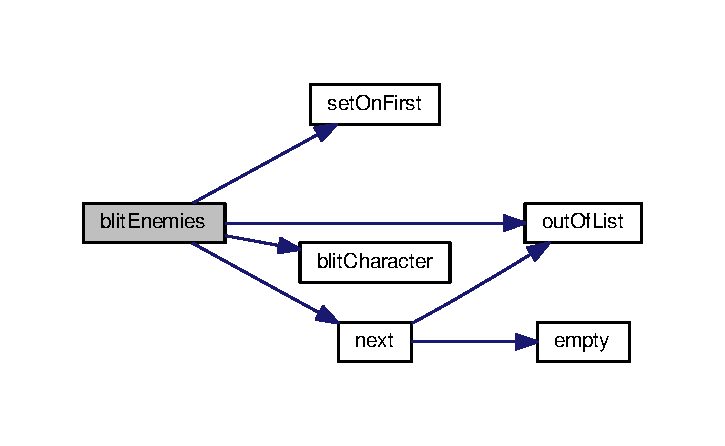
\includegraphics[width=348pt]{enemies_8h_ada7bfd5ddcfd60cd52ad17b2c9b37b8f_cgraph}
\end{center}
\end{figure}


\hypertarget{enemies_8h_ae36bc711341ade0e08eb57e1c5063174}{\index{enemies.\-h@{enemies.\-h}!collision\-Enemy@{collision\-Enemy}}
\index{collision\-Enemy@{collision\-Enemy}!enemies.h@{enemies.\-h}}
\paragraph[{collision\-Enemy}]{\setlength{\rightskip}{0pt plus 5cm}int collision\-Enemy (
\begin{DoxyParamCaption}
\item[{{\bf Character} $\ast$}]{c, }
\item[{{\bf list} $\ast$}]{l, }
\item[{{\bf Map} $\ast$}]{m}
\end{DoxyParamCaption}
)}}\label{enemies_8h_ae36bc711341ade0e08eb57e1c5063174}
determine if there is a collision beteewen the player sprite and an enemy and deals with 
\begin{DoxyParams}[1]{Parameters}
\mbox{\tt in,out}  & {\em c} & the player \\
\hline
\mbox{\tt in,out}  & {\em l} & the enemy list, change the current node \\
\hline
\mbox{\tt in}  & {\em m} & the game map \\
\hline
\end{DoxyParams}
\begin{DoxyReturn}{Returns}
1 if there is a collision, 0 if not 
\end{DoxyReturn}


Here is the call graph for this function\-:\nopagebreak
\begin{figure}[H]
\begin{center}
\leavevmode
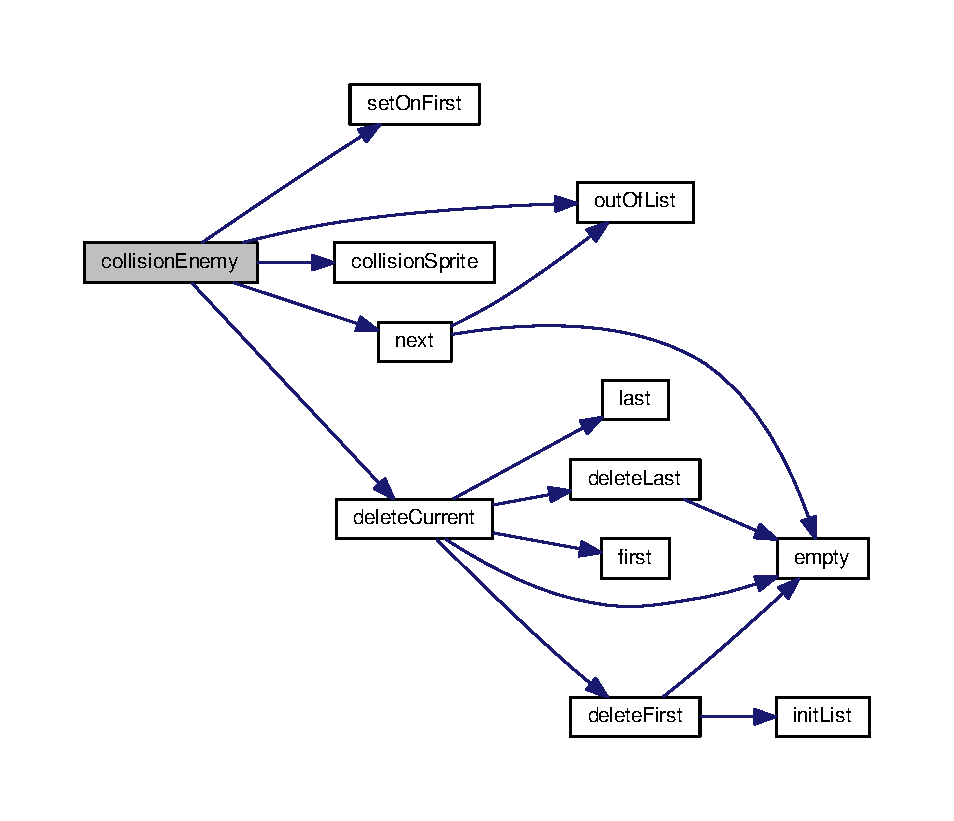
\includegraphics[width=350pt]{enemies_8h_ae36bc711341ade0e08eb57e1c5063174_cgraph}
\end{center}
\end{figure}


\hypertarget{enemies_8h_a68e86bc615a3b71cf549b32a71f6c943}{\index{enemies.\-h@{enemies.\-h}!create\-Enemy@{create\-Enemy}}
\index{create\-Enemy@{create\-Enemy}!enemies.h@{enemies.\-h}}
\paragraph[{create\-Enemy}]{\setlength{\rightskip}{0pt plus 5cm}void create\-Enemy (
\begin{DoxyParamCaption}
\item[{char $\ast$}]{tile, }
\item[{int}]{x, }
\item[{int}]{y, }
\item[{{\bf list} $\ast$}]{l, }
\item[{int}]{type}
\end{DoxyParamCaption}
)}}\label{enemies_8h_a68e86bc615a3b71cf549b32a71f6c943}
creates an enemy and adds it to an enemies list 
\begin{DoxyParams}[1]{Parameters}
\mbox{\tt in}  & {\em tile} & the tilset name \\
\hline
\mbox{\tt in}  & {\em x} & enemy's x location \\
\hline
\mbox{\tt in}  & {\em y} & enemy's y location \\
\hline
\mbox{\tt out}  & {\em l} & enemies list \\
\hline
\mbox{\tt in}  & {\em type} & the type of enemy \\
\hline
\end{DoxyParams}


Here is the call graph for this function\-:\nopagebreak
\begin{figure}[H]
\begin{center}
\leavevmode
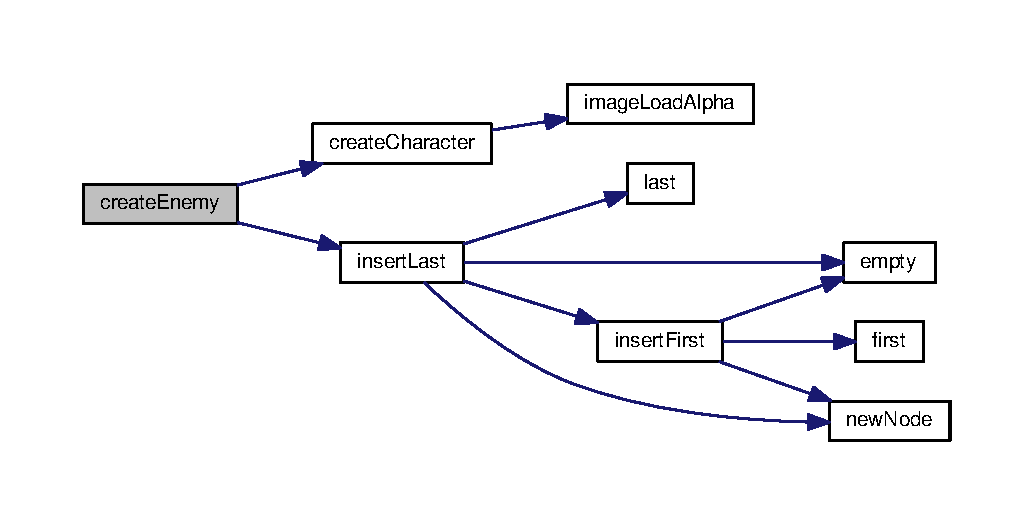
\includegraphics[width=350pt]{enemies_8h_a68e86bc615a3b71cf549b32a71f6c943_cgraph}
\end{center}
\end{figure}


\hypertarget{enemies_8h_ac507237248dd8833577460bb908e100b}{\index{enemies.\-h@{enemies.\-h}!delete\-Current@{delete\-Current}}
\index{delete\-Current@{delete\-Current}!enemies.h@{enemies.\-h}}
\paragraph[{delete\-Current}]{\setlength{\rightskip}{0pt plus 5cm}{\bf Character}$\ast$ delete\-Current (
\begin{DoxyParamCaption}
\item[{{\bf list} $\ast$}]{l}
\end{DoxyParamCaption}
)}}\label{enemies_8h_ac507237248dd8833577460bb908e100b}
delete the current node 
\begin{DoxyParams}[1]{Parameters}
\mbox{\tt out}  & {\em l} & the list which has to be modified \\
\hline
\end{DoxyParams}
\begin{DoxyReturn}{Returns}
the current node's enemy, N\-U\-L\-L if empty list 
\end{DoxyReturn}


Here is the call graph for this function\-:\nopagebreak
\begin{figure}[H]
\begin{center}
\leavevmode
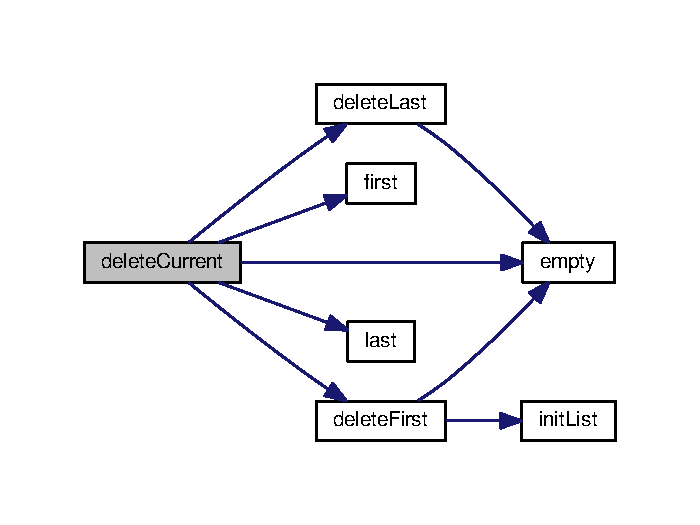
\includegraphics[width=336pt]{enemies_8h_ac507237248dd8833577460bb908e100b_cgraph}
\end{center}
\end{figure}


\hypertarget{enemies_8h_a194e361c113eeffdd25fc8726b3c000d}{\index{enemies.\-h@{enemies.\-h}!delete\-First@{delete\-First}}
\index{delete\-First@{delete\-First}!enemies.h@{enemies.\-h}}
\paragraph[{delete\-First}]{\setlength{\rightskip}{0pt plus 5cm}{\bf Character}$\ast$ delete\-First (
\begin{DoxyParamCaption}
\item[{{\bf list} $\ast$}]{l}
\end{DoxyParamCaption}
)}}\label{enemies_8h_a194e361c113eeffdd25fc8726b3c000d}
delete the first node 
\begin{DoxyParams}[1]{Parameters}
\mbox{\tt out}  & {\em l} & the list which has to be modified \\
\hline
\end{DoxyParams}
\begin{DoxyReturn}{Returns}
the first node's enemy, N\-U\-L\-L if empty list 
\end{DoxyReturn}


Here is the call graph for this function\-:\nopagebreak
\begin{figure}[H]
\begin{center}
\leavevmode
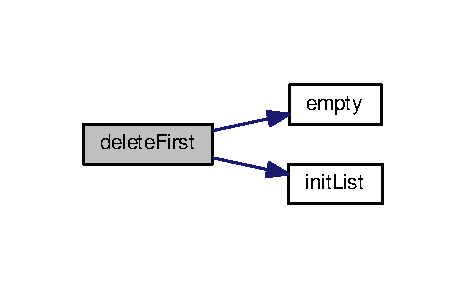
\includegraphics[width=224pt]{enemies_8h_a194e361c113eeffdd25fc8726b3c000d_cgraph}
\end{center}
\end{figure}


\hypertarget{enemies_8h_ae1ba17d62391833365fa4462690b31c5}{\index{enemies.\-h@{enemies.\-h}!delete\-Last@{delete\-Last}}
\index{delete\-Last@{delete\-Last}!enemies.h@{enemies.\-h}}
\paragraph[{delete\-Last}]{\setlength{\rightskip}{0pt plus 5cm}{\bf Character}$\ast$ delete\-Last (
\begin{DoxyParamCaption}
\item[{{\bf list} $\ast$}]{l}
\end{DoxyParamCaption}
)}}\label{enemies_8h_ae1ba17d62391833365fa4462690b31c5}
delete the last node 
\begin{DoxyParams}[1]{Parameters}
\mbox{\tt out}  & {\em l} & the list which has to be modified \\
\hline
\end{DoxyParams}
\begin{DoxyReturn}{Returns}
the last node's enemy, N\-U\-L\-L if empty list 
\end{DoxyReturn}


Here is the call graph for this function\-:\nopagebreak
\begin{figure}[H]
\begin{center}
\leavevmode
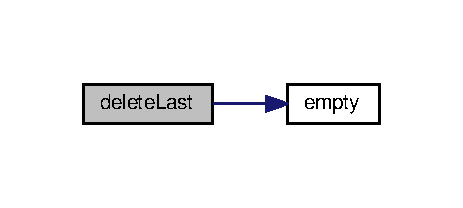
\includegraphics[width=222pt]{enemies_8h_ae1ba17d62391833365fa4462690b31c5_cgraph}
\end{center}
\end{figure}


\hypertarget{enemies_8h_a185b7dd5b77fdf2b6315358ac7767e44}{\index{enemies.\-h@{enemies.\-h}!empty@{empty}}
\index{empty@{empty}!enemies.h@{enemies.\-h}}
\paragraph[{empty}]{\setlength{\rightskip}{0pt plus 5cm}int empty (
\begin{DoxyParamCaption}
\item[{{\bf list} $\ast$}]{l}
\end{DoxyParamCaption}
)}}\label{enemies_8h_a185b7dd5b77fdf2b6315358ac7767e44}
tests if the list is empty 
\begin{DoxyParams}[1]{Parameters}
\mbox{\tt in}  & {\em l} & the list to be tested \\
\hline
\end{DoxyParams}
\begin{DoxyReturn}{Returns}
1 if the list is empty, 0 if not 
\end{DoxyReturn}
\hypertarget{enemies_8h_a0f5c139f75d0a54b38c0d33e1bc22223}{\index{enemies.\-h@{enemies.\-h}!first@{first}}
\index{first@{first}!enemies.h@{enemies.\-h}}
\paragraph[{first}]{\setlength{\rightskip}{0pt plus 5cm}int first (
\begin{DoxyParamCaption}
\item[{{\bf list} $\ast$}]{l}
\end{DoxyParamCaption}
)}}\label{enemies_8h_a0f5c139f75d0a54b38c0d33e1bc22223}
tests if the current node is the first node 
\begin{DoxyParams}[1]{Parameters}
\mbox{\tt in}  & {\em l} & the list to be tested \\
\hline
\end{DoxyParams}
\begin{DoxyReturn}{Returns}
1 if the current node is the first node, 0 if not 
\end{DoxyReturn}
\hypertarget{enemies_8h_a766e049c933ace6a69ba1e7c3fab142c}{\index{enemies.\-h@{enemies.\-h}!free\-Enemies@{free\-Enemies}}
\index{free\-Enemies@{free\-Enemies}!enemies.h@{enemies.\-h}}
\paragraph[{free\-Enemies}]{\setlength{\rightskip}{0pt plus 5cm}void free\-Enemies (
\begin{DoxyParamCaption}
\item[{{\bf list} $\ast$}]{l}
\end{DoxyParamCaption}
)}}\label{enemies_8h_a766e049c933ace6a69ba1e7c3fab142c}
free all the enemies and the list 
\begin{DoxyParams}[1]{Parameters}
\mbox{\tt out}  & {\em l} & the enemy list \\
\hline
\end{DoxyParams}


Here is the call graph for this function\-:\nopagebreak
\begin{figure}[H]
\begin{center}
\leavevmode
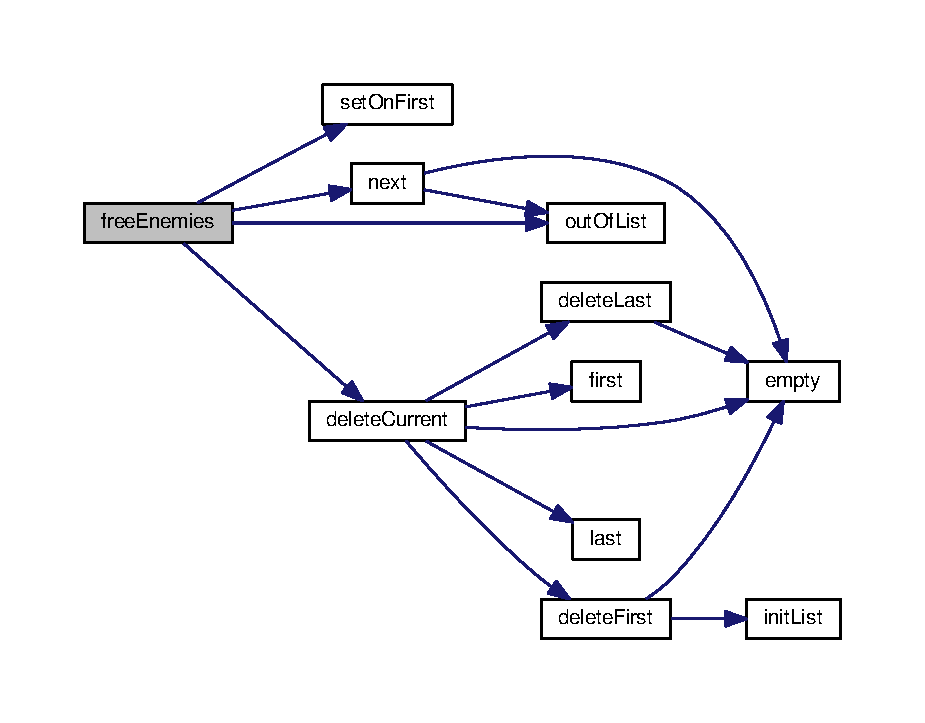
\includegraphics[width=350pt]{enemies_8h_a766e049c933ace6a69ba1e7c3fab142c_cgraph}
\end{center}
\end{figure}


\hypertarget{enemies_8h_a38ef80c447f07fdd6319ab28fd5dc7da}{\index{enemies.\-h@{enemies.\-h}!get\-Current@{get\-Current}}
\index{get\-Current@{get\-Current}!enemies.h@{enemies.\-h}}
\paragraph[{get\-Current}]{\setlength{\rightskip}{0pt plus 5cm}{\bf Character}$\ast$ get\-Current (
\begin{DoxyParamCaption}
\item[{{\bf list} $\ast$}]{l}
\end{DoxyParamCaption}
)}}\label{enemies_8h_a38ef80c447f07fdd6319ab28fd5dc7da}
get the character of the current node 
\begin{DoxyParams}[1]{Parameters}
\mbox{\tt in}  & {\em l} & the list to be modified \\
\hline
\end{DoxyParams}
\hypertarget{enemies_8h_aaca0e3ca99177d70268a1f770c50e264}{\index{enemies.\-h@{enemies.\-h}!init\-List@{init\-List}}
\index{init\-List@{init\-List}!enemies.h@{enemies.\-h}}
\paragraph[{init\-List}]{\setlength{\rightskip}{0pt plus 5cm}void init\-List (
\begin{DoxyParamCaption}
\item[{{\bf list} $\ast$}]{l}
\end{DoxyParamCaption}
)}}\label{enemies_8h_aaca0e3ca99177d70268a1f770c50e264}
initialize the enemy list 
\begin{DoxyParams}[1]{Parameters}
\mbox{\tt out}  & {\em l} & the list to be initalized \\
\hline
\end{DoxyParams}
\hypertarget{enemies_8h_ae745be19268624b512665dce384c7eb4}{\index{enemies.\-h@{enemies.\-h}!insert\-After\-Current@{insert\-After\-Current}}
\index{insert\-After\-Current@{insert\-After\-Current}!enemies.h@{enemies.\-h}}
\paragraph[{insert\-After\-Current}]{\setlength{\rightskip}{0pt plus 5cm}int insert\-After\-Current (
\begin{DoxyParamCaption}
\item[{{\bf list} $\ast$}]{l, }
\item[{{\bf Character} $\ast$}]{c}
\end{DoxyParamCaption}
)}}\label{enemies_8h_ae745be19268624b512665dce384c7eb4}
insert a enemy just after the current node 
\begin{DoxyParams}[1]{Parameters}
\mbox{\tt out}  & {\em l} & the list in which the enemy has to be inserted \\
\hline
\mbox{\tt in}  & {\em c} & the character to be inserted \\
\hline
\end{DoxyParams}
\begin{DoxyReturn}{Returns}
1 if enemy inserted, 0 if failure 
\end{DoxyReturn}


Here is the call graph for this function\-:\nopagebreak
\begin{figure}[H]
\begin{center}
\leavevmode
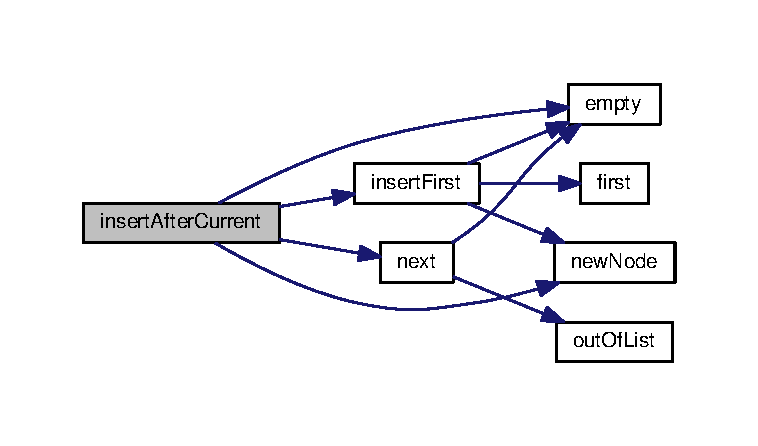
\includegraphics[width=350pt]{enemies_8h_ae745be19268624b512665dce384c7eb4_cgraph}
\end{center}
\end{figure}


\hypertarget{enemies_8h_ae8c5bac4a4363592b055b0cd4000864c}{\index{enemies.\-h@{enemies.\-h}!insert\-Before\-Current@{insert\-Before\-Current}}
\index{insert\-Before\-Current@{insert\-Before\-Current}!enemies.h@{enemies.\-h}}
\paragraph[{insert\-Before\-Current}]{\setlength{\rightskip}{0pt plus 5cm}int insert\-Before\-Current (
\begin{DoxyParamCaption}
\item[{{\bf list} $\ast$}]{l, }
\item[{{\bf Character} $\ast$}]{c}
\end{DoxyParamCaption}
)}}\label{enemies_8h_ae8c5bac4a4363592b055b0cd4000864c}
insert a enemy just before the current node 
\begin{DoxyParams}[1]{Parameters}
\mbox{\tt out}  & {\em l} & the list in which the enemy has to be inserted \\
\hline
\mbox{\tt in}  & {\em c} & the character to be inserted \\
\hline
\end{DoxyParams}
\begin{DoxyReturn}{Returns}
1 if enemy inserted, 0 if failure 
\end{DoxyReturn}


Here is the call graph for this function\-:\nopagebreak
\begin{figure}[H]
\begin{center}
\leavevmode
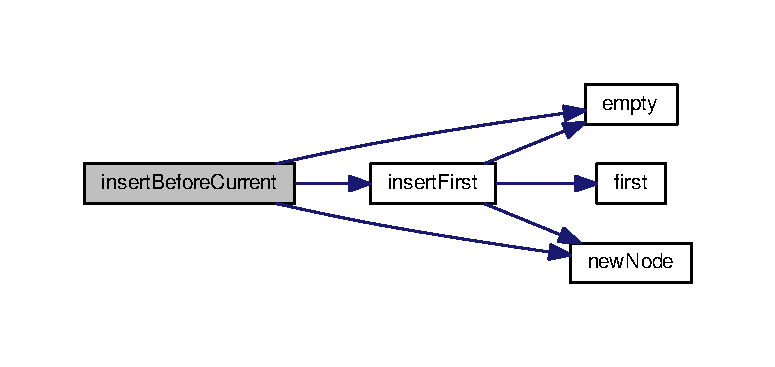
\includegraphics[width=350pt]{enemies_8h_ae8c5bac4a4363592b055b0cd4000864c_cgraph}
\end{center}
\end{figure}


\hypertarget{enemies_8h_a277ce428e10c4d50abdae6d162128f48}{\index{enemies.\-h@{enemies.\-h}!insert\-First@{insert\-First}}
\index{insert\-First@{insert\-First}!enemies.h@{enemies.\-h}}
\paragraph[{insert\-First}]{\setlength{\rightskip}{0pt plus 5cm}int insert\-First (
\begin{DoxyParamCaption}
\item[{{\bf list} $\ast$}]{l, }
\item[{{\bf Character} $\ast$}]{c}
\end{DoxyParamCaption}
)}}\label{enemies_8h_a277ce428e10c4d50abdae6d162128f48}
insert a enemy as first node 
\begin{DoxyParams}[1]{Parameters}
\mbox{\tt out}  & {\em l} & the list in which the enemy has to be inserted \\
\hline
\mbox{\tt in}  & {\em c} & the charcter to be inserted \\
\hline
\end{DoxyParams}
\begin{DoxyReturn}{Returns}
1 if enemy inserted, 0 if failure 
\end{DoxyReturn}


Here is the call graph for this function\-:\nopagebreak
\begin{figure}[H]
\begin{center}
\leavevmode
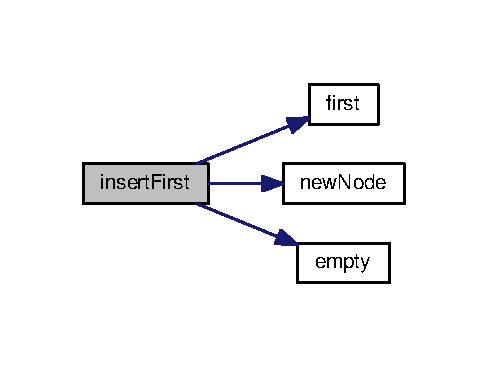
\includegraphics[width=234pt]{enemies_8h_a277ce428e10c4d50abdae6d162128f48_cgraph}
\end{center}
\end{figure}


\hypertarget{enemies_8h_a121944b1f370af47e1f980128bf0fc86}{\index{enemies.\-h@{enemies.\-h}!insert\-Last@{insert\-Last}}
\index{insert\-Last@{insert\-Last}!enemies.h@{enemies.\-h}}
\paragraph[{insert\-Last}]{\setlength{\rightskip}{0pt plus 5cm}int insert\-Last (
\begin{DoxyParamCaption}
\item[{{\bf list} $\ast$}]{l, }
\item[{{\bf Character} $\ast$}]{c}
\end{DoxyParamCaption}
)}}\label{enemies_8h_a121944b1f370af47e1f980128bf0fc86}
insert a enemy as last node 
\begin{DoxyParams}[1]{Parameters}
\mbox{\tt out}  & {\em l} & the list in which the enemy has to be inserted \\
\hline
\mbox{\tt in}  & {\em c} & the character to be inserted \\
\hline
\end{DoxyParams}
\begin{DoxyReturn}{Returns}
1 if enemy inserted, 0 if failure 
\end{DoxyReturn}


Here is the call graph for this function\-:\nopagebreak
\begin{figure}[H]
\begin{center}
\leavevmode
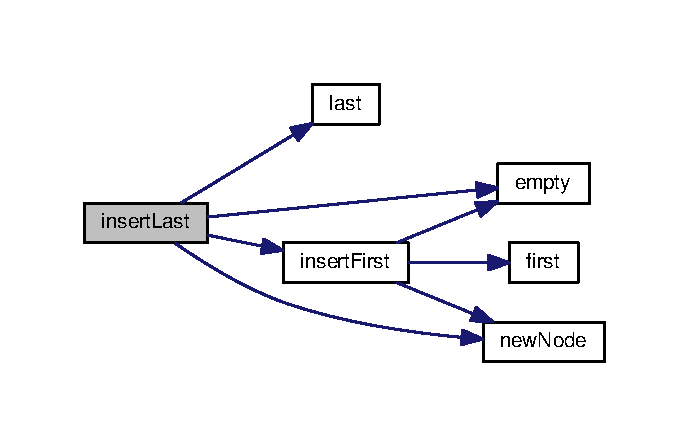
\includegraphics[width=330pt]{enemies_8h_a121944b1f370af47e1f980128bf0fc86_cgraph}
\end{center}
\end{figure}


\hypertarget{enemies_8h_a86d339159e440962ce42347b99e07625}{\index{enemies.\-h@{enemies.\-h}!last@{last}}
\index{last@{last}!enemies.h@{enemies.\-h}}
\paragraph[{last}]{\setlength{\rightskip}{0pt plus 5cm}int last (
\begin{DoxyParamCaption}
\item[{{\bf list} $\ast$}]{l}
\end{DoxyParamCaption}
)}}\label{enemies_8h_a86d339159e440962ce42347b99e07625}
tests if the current node is the last node 
\begin{DoxyParams}[1]{Parameters}
\mbox{\tt in}  & {\em l} & the list to be tested \\
\hline
\end{DoxyParams}
\begin{DoxyReturn}{Returns}
1 if the current node is the last node, 0 if not 
\end{DoxyReturn}
\hypertarget{enemies_8h_a315db1acddbe1cd18db63bab85f1709a}{\index{enemies.\-h@{enemies.\-h}!move\-Character\-Col@{move\-Character\-Col}}
\index{move\-Character\-Col@{move\-Character\-Col}!enemies.h@{enemies.\-h}}
\paragraph[{move\-Character\-Col}]{\setlength{\rightskip}{0pt plus 5cm}int move\-Character\-Col (
\begin{DoxyParamCaption}
\item[{{\bf Character} $\ast$}]{c, }
\item[{int}]{move\-\_\-left, }
\item[{int}]{move\-\_\-right, }
\item[{{\bf Map} $\ast$}]{m}
\end{DoxyParamCaption}
)}}\label{enemies_8h_a315db1acddbe1cd18db63bab85f1709a}
moves the character if it's hurt by an enemy 
\begin{DoxyParams}[1]{Parameters}
\mbox{\tt in,out}  & {\em c} & the character \\
\hline
\mbox{\tt in,out}  & {\em move\-\_\-left} & indicate if the character must move left \\
\hline
\mbox{\tt in,out}  & {\em move\-\_\-right} & indicate if the character must move right \\
\hline
\mbox{\tt in}  & {\em m} & level map \\
\hline
\end{DoxyParams}
\begin{DoxyReturn}{Returns}
1 if character was moved without using the precise movement function, 0 if not 
\end{DoxyReturn}


Here is the call graph for this function\-:\nopagebreak
\begin{figure}[H]
\begin{center}
\leavevmode
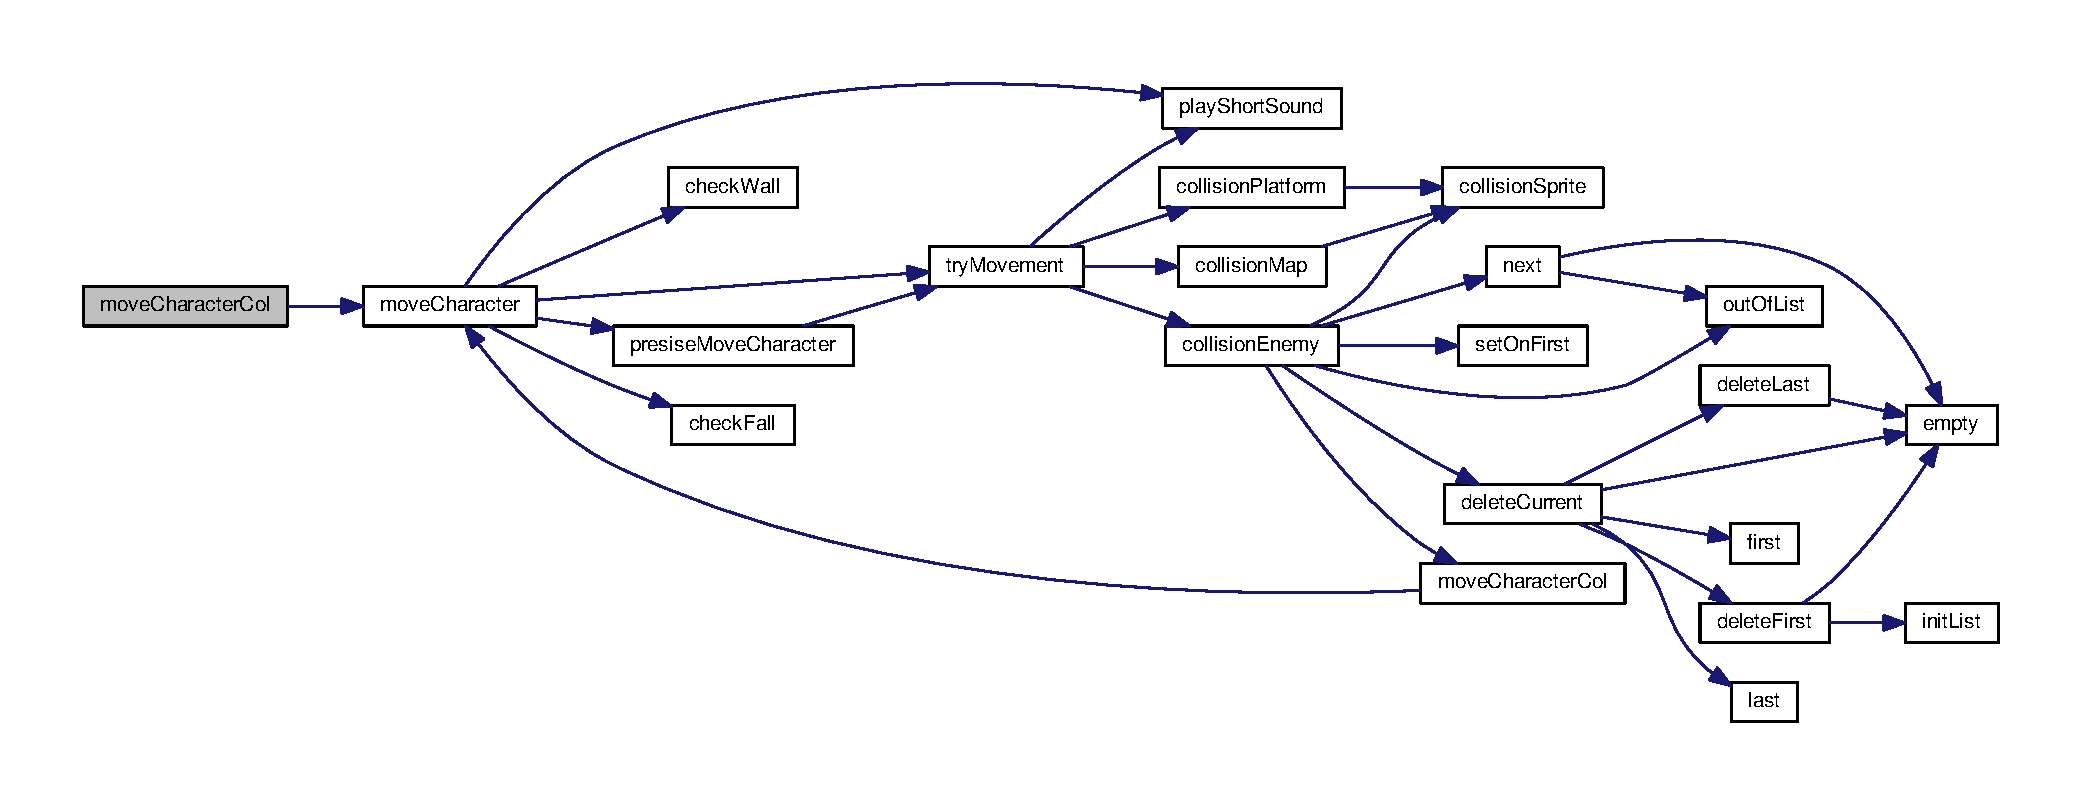
\includegraphics[width=350pt]{enemies_8h_a315db1acddbe1cd18db63bab85f1709a_cgraph}
\end{center}
\end{figure}


\hypertarget{enemies_8h_a5cc0822e34be00f2555f70f8acf17680}{\index{enemies.\-h@{enemies.\-h}!move\-Enemies@{move\-Enemies}}
\index{move\-Enemies@{move\-Enemies}!enemies.h@{enemies.\-h}}
\paragraph[{move\-Enemies}]{\setlength{\rightskip}{0pt plus 5cm}void move\-Enemies (
\begin{DoxyParamCaption}
\item[{{\bf list} $\ast$}]{l, }
\item[{{\bf Map} $\ast$}]{m, }
\item[{{\bf list} $\ast$}]{p, }
\item[{{\bf projectile\-Set} $\ast$}]{ps, }
\item[{int $\ast$}]{launch}
\end{DoxyParamCaption}
)}}\label{enemies_8h_a5cc0822e34be00f2555f70f8acf17680}
make the enemies moving 
\begin{DoxyParams}[1]{Parameters}
\mbox{\tt in,out}  & {\em l} & the enemy list \\
\hline
\mbox{\tt in}  & {\em m} & the game map \\
\hline
\mbox{\tt in,out}  & {\em p} & the player list \\
\hline
\mbox{\tt out}  & {\em ps} & the projectile set \\
\hline
\mbox{\tt in}  & {\em launch} & if 1, canons can fire an rocket \\
\hline
\end{DoxyParams}


Here is the call graph for this function\-:\nopagebreak
\begin{figure}[H]
\begin{center}
\leavevmode
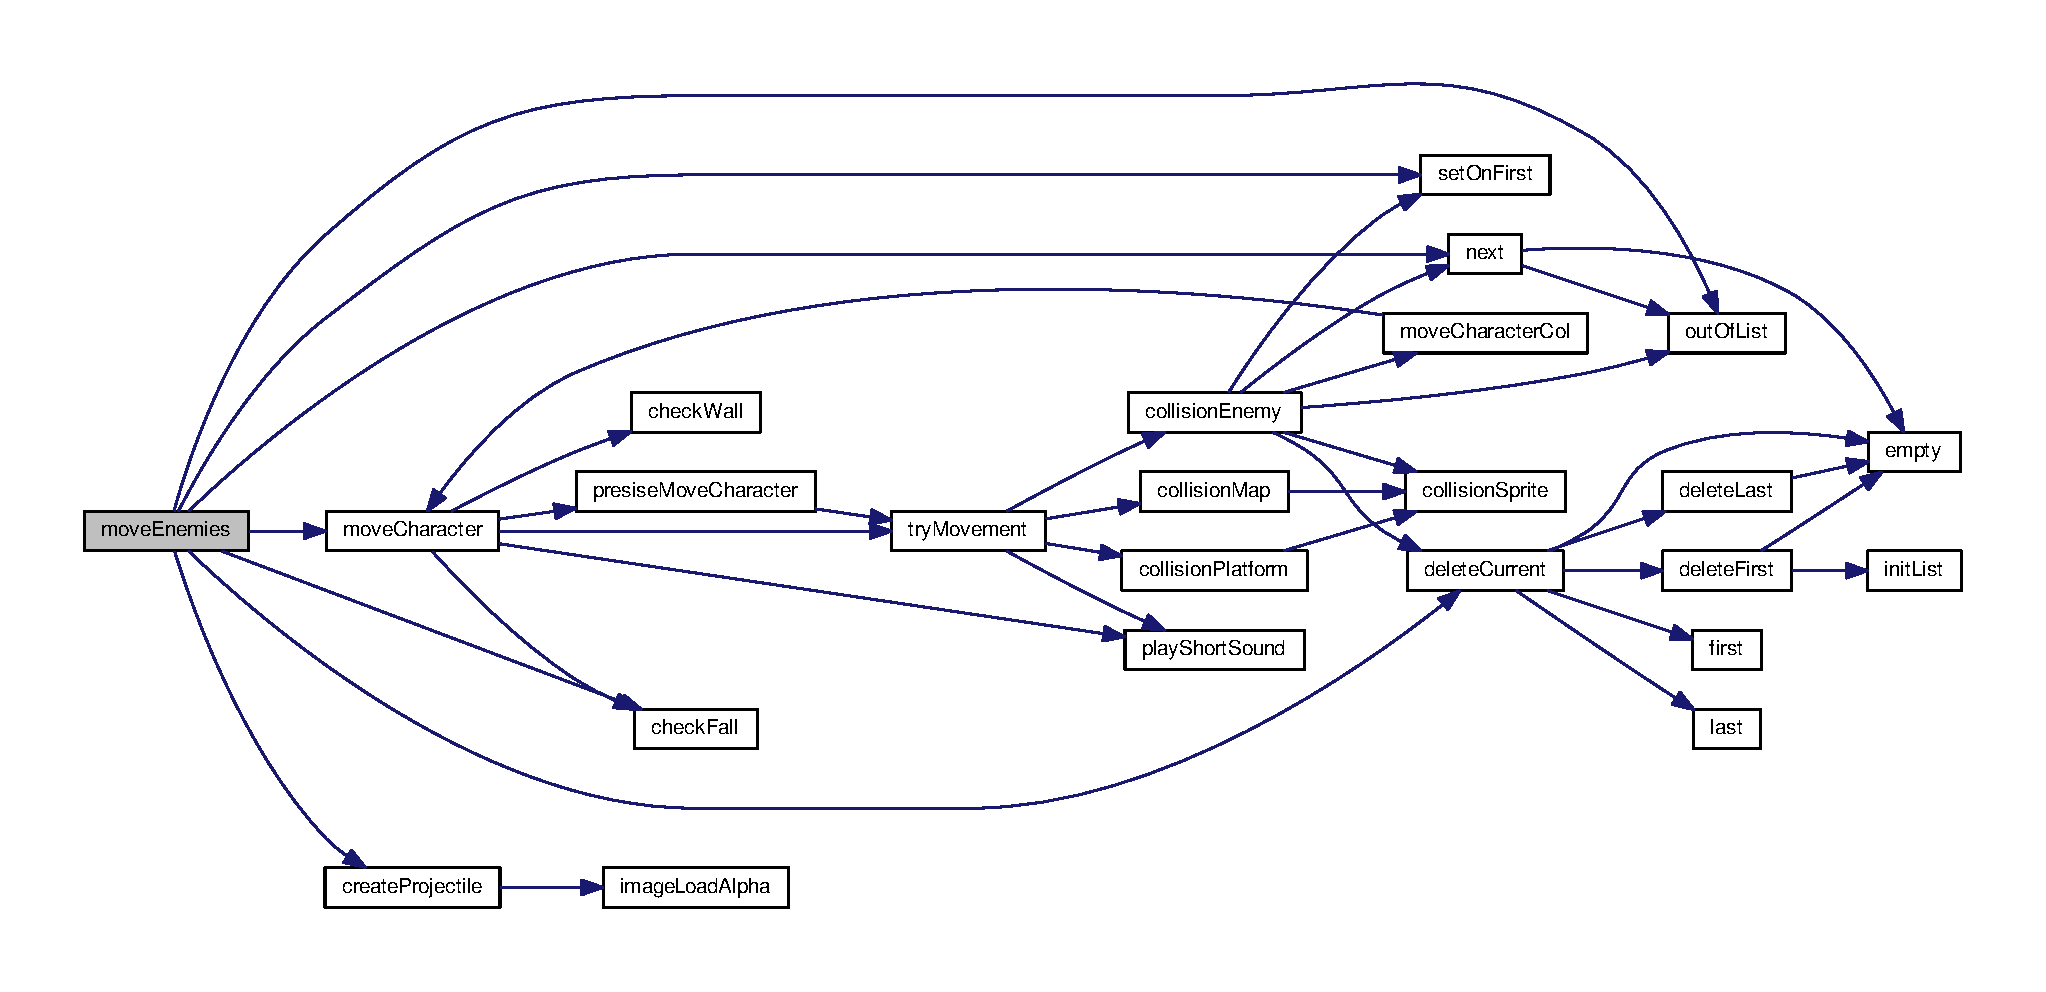
\includegraphics[width=350pt]{enemies_8h_a5cc0822e34be00f2555f70f8acf17680_cgraph}
\end{center}
\end{figure}


\hypertarget{enemies_8h_a86da34107b65b23bb7105568af701160}{\index{enemies.\-h@{enemies.\-h}!new\-Node@{new\-Node}}
\index{new\-Node@{new\-Node}!enemies.h@{enemies.\-h}}
\paragraph[{new\-Node}]{\setlength{\rightskip}{0pt plus 5cm}{\bf node}$\ast$ new\-Node (
\begin{DoxyParamCaption}
\item[{{\bf Character} $\ast$}]{c, }
\item[{{\bf node} $\ast$}]{n, }
\item[{{\bf node} $\ast$}]{p}
\end{DoxyParamCaption}
)}}\label{enemies_8h_a86da34107b65b23bb7105568af701160}
creates a new node 
\begin{DoxyParams}[1]{Parameters}
\mbox{\tt in}  & {\em c} & the character of the node \\
\hline
\mbox{\tt in}  & {\em n} & the next node \\
\hline
\mbox{\tt in}  & {\em p} & the previous node \\
\hline
\end{DoxyParams}
\begin{DoxyReturn}{Returns}
a pointer on the created node 
\end{DoxyReturn}
\hypertarget{enemies_8h_a1e9424bcb6302d001589f04a99802abf}{\index{enemies.\-h@{enemies.\-h}!next@{next}}
\index{next@{next}!enemies.h@{enemies.\-h}}
\paragraph[{next}]{\setlength{\rightskip}{0pt plus 5cm}void next (
\begin{DoxyParamCaption}
\item[{{\bf list} $\ast$}]{l}
\end{DoxyParamCaption}
)}}\label{enemies_8h_a1e9424bcb6302d001589f04a99802abf}
set the current node on its next node 
\begin{DoxyParams}[1]{Parameters}
\mbox{\tt out}  & {\em l} & the list to be modified \\
\hline
\end{DoxyParams}


Here is the call graph for this function\-:\nopagebreak
\begin{figure}[H]
\begin{center}
\leavevmode
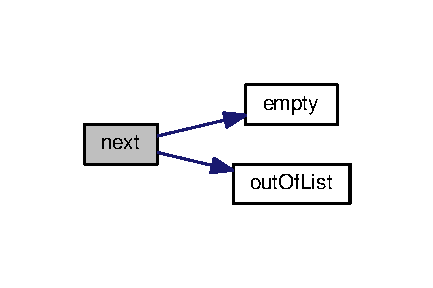
\includegraphics[width=208pt]{enemies_8h_a1e9424bcb6302d001589f04a99802abf_cgraph}
\end{center}
\end{figure}


\hypertarget{enemies_8h_a7774be61944dce2ae021e0e4442b4515}{\index{enemies.\-h@{enemies.\-h}!out\-Of\-List@{out\-Of\-List}}
\index{out\-Of\-List@{out\-Of\-List}!enemies.h@{enemies.\-h}}
\paragraph[{out\-Of\-List}]{\setlength{\rightskip}{0pt plus 5cm}int out\-Of\-List (
\begin{DoxyParamCaption}
\item[{{\bf list} $\ast$}]{l}
\end{DoxyParamCaption}
)}}\label{enemies_8h_a7774be61944dce2ae021e0e4442b4515}
tests if the current node is in the list 
\begin{DoxyParams}[1]{Parameters}
\mbox{\tt in}  & {\em l} & the list to be tested \\
\hline
\end{DoxyParams}
\begin{DoxyReturn}{Returns}
1 if the current node is in the list, 0 if not 
\end{DoxyReturn}
\hypertarget{enemies_8h_ab6a55e4b951590640debd7d4110c37e6}{\index{enemies.\-h@{enemies.\-h}!previous@{previous}}
\index{previous@{previous}!enemies.h@{enemies.\-h}}
\paragraph[{previous}]{\setlength{\rightskip}{0pt plus 5cm}void previous (
\begin{DoxyParamCaption}
\item[{{\bf list} $\ast$}]{l}
\end{DoxyParamCaption}
)}}\label{enemies_8h_ab6a55e4b951590640debd7d4110c37e6}
set the current node on its previous node 
\begin{DoxyParams}[1]{Parameters}
\mbox{\tt out}  & {\em l} & the list to be modified \\
\hline
\end{DoxyParams}
\hypertarget{enemies_8h_aa0ae9a01476366cb08c3e904e2f31433}{\index{enemies.\-h@{enemies.\-h}!set\-On\-First@{set\-On\-First}}
\index{set\-On\-First@{set\-On\-First}!enemies.h@{enemies.\-h}}
\paragraph[{set\-On\-First}]{\setlength{\rightskip}{0pt plus 5cm}void set\-On\-First (
\begin{DoxyParamCaption}
\item[{{\bf list} $\ast$}]{l}
\end{DoxyParamCaption}
)}}\label{enemies_8h_aa0ae9a01476366cb08c3e904e2f31433}
set the current node on the first node 
\begin{DoxyParams}[1]{Parameters}
\mbox{\tt out}  & {\em l} & the list to be modified \\
\hline
\end{DoxyParams}
\hypertarget{enemies_8h_ad8a2ca1098f3a37401100bf88c3a4f03}{\index{enemies.\-h@{enemies.\-h}!set\-On\-Last@{set\-On\-Last}}
\index{set\-On\-Last@{set\-On\-Last}!enemies.h@{enemies.\-h}}
\paragraph[{set\-On\-Last}]{\setlength{\rightskip}{0pt plus 5cm}void set\-On\-Last (
\begin{DoxyParamCaption}
\item[{{\bf list} $\ast$}]{l}
\end{DoxyParamCaption}
)}}\label{enemies_8h_ad8a2ca1098f3a37401100bf88c3a4f03}
set the current node on the last node 
\begin{DoxyParams}[1]{Parameters}
\mbox{\tt out}  & {\em l} & the list to be modified \\
\hline
\end{DoxyParams}

\hypertarget{file_8c}{\section{file.\-c File Reference}
\label{file_8c}\index{file.\-c@{file.\-c}}
}


file access functions  


{\ttfamily \#include \char`\"{}file.\-h\char`\"{}}\\*
Include dependency graph for file.\-c\-:\nopagebreak
\begin{figure}[H]
\begin{center}
\leavevmode
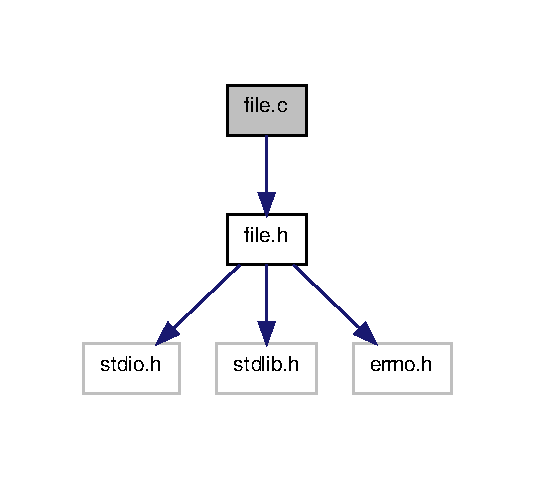
\includegraphics[width=256pt]{file_8c__incl}
\end{center}
\end{figure}
\subsection*{Functions}
\begin{DoxyCompactItemize}
\item 
F\-I\-L\-E $\ast$ \hyperlink{file_8c_ab763060cbdd57fdb704871d896fc492a}{open\-File} (char name\mbox{[}$\,$\mbox{]}, char mode\mbox{[}$\,$\mbox{]})
\item 
int \hyperlink{file_8c_adf55ac6bc5d81f94b54e4c8ea554f884}{close\-File} (F\-I\-L\-E $\ast$ptr\-\_\-file)
\end{DoxyCompactItemize}


\subsection{Detailed Description}
file access functions \begin{DoxyAuthor}{Author}
Remi B\-E\-R\-T\-H\-O 
\end{DoxyAuthor}
\begin{DoxyDate}{Date}
15/03/14 
\end{DoxyDate}


\subsection{Function Documentation}
\hypertarget{file_8c_adf55ac6bc5d81f94b54e4c8ea554f884}{\index{file.\-c@{file.\-c}!close\-File@{close\-File}}
\index{close\-File@{close\-File}!file.c@{file.\-c}}
\subsubsection[{close\-File}]{\setlength{\rightskip}{0pt plus 5cm}int close\-File (
\begin{DoxyParamCaption}
\item[{F\-I\-L\-E $\ast$}]{ptr\-\_\-file}
\end{DoxyParamCaption}
)}}\label{file_8c_adf55ac6bc5d81f94b54e4c8ea554f884}
close a file 
\begin{DoxyParams}[1]{Parameters}
\mbox{\tt in}  & {\em $\ast$ptr\-\_\-file} & the file to be closed \\
\hline
\end{DoxyParams}
\begin{DoxyReturn}{Returns}
int 0 if the file was succefuly closed, 1 if not 
\end{DoxyReturn}
\hypertarget{file_8c_ab763060cbdd57fdb704871d896fc492a}{\index{file.\-c@{file.\-c}!open\-File@{open\-File}}
\index{open\-File@{open\-File}!file.c@{file.\-c}}
\subsubsection[{open\-File}]{\setlength{\rightskip}{0pt plus 5cm}F\-I\-L\-E $\ast$ open\-File (
\begin{DoxyParamCaption}
\item[{char}]{name\mbox{[}$\,$\mbox{]}, }
\item[{char}]{mode\mbox{[}$\,$\mbox{]}}
\end{DoxyParamCaption}
)}}\label{file_8c_ab763060cbdd57fdb704871d896fc492a}
open a file 
\begin{DoxyParams}[1]{Parameters}
\mbox{\tt in}  & {\em name} & the file name/path \\
\hline
\mbox{\tt in}  & {\em mode} & the opening mode \\
\hline
\end{DoxyParams}
\begin{DoxyReturn}{Returns}
a pointer on the opened file, N\-U\-L\-L if error 
\end{DoxyReturn}

\hypertarget{file_8h}{\subsection{file.\-h File Reference}
\label{file_8h}\index{file.\-h@{file.\-h}}
}


\hyperlink{file_8c}{file.\-c} header  


{\ttfamily \#include $<$stdio.\-h$>$}\\*
{\ttfamily \#include $<$stdlib.\-h$>$}\\*
{\ttfamily \#include $<$errno.\-h$>$}\\*
\subsubsection*{Functions}
\begin{DoxyCompactItemize}
\item 
F\-I\-L\-E $\ast$ \hyperlink{file_8h_ae6218cf222b5ca17dce1ad7eb75346a9}{open\-File} (char nome\mbox{[}$\,$\mbox{]}, char mode\mbox{[}$\,$\mbox{]})
\item 
int \hyperlink{file_8h_a0fca34d72624f611d2cbeac47279bb1f}{close\-File} (F\-I\-L\-E $\ast$ptr\-\_\-fichier)
\end{DoxyCompactItemize}


\subsubsection{Detailed Description}
\hyperlink{file_8c}{file.\-c} header \begin{DoxyAuthor}{Author}
Remi B\-E\-R\-T\-H\-O, Glenn H\-E\-R\-R\-O\-U 
\end{DoxyAuthor}
\begin{DoxyDate}{Date}
2014-\/05-\/12 
\end{DoxyDate}


\subsubsection{Function Documentation}
\hypertarget{file_8h_a0fca34d72624f611d2cbeac47279bb1f}{\index{file.\-h@{file.\-h}!close\-File@{close\-File}}
\index{close\-File@{close\-File}!file.h@{file.\-h}}
\paragraph[{close\-File}]{\setlength{\rightskip}{0pt plus 5cm}int close\-File (
\begin{DoxyParamCaption}
\item[{F\-I\-L\-E $\ast$}]{ptr\-\_\-file}
\end{DoxyParamCaption}
)}}\label{file_8h_a0fca34d72624f611d2cbeac47279bb1f}
Close the given file 
\begin{DoxyParams}[1]{Parameters}
\mbox{\tt in}  & {\em $\ast$ptr\-\_\-file} & the file \\
\hline
\end{DoxyParams}
\begin{DoxyReturn}{Returns}
0 if the file has been succesfully closed, 1 otherwise 
\end{DoxyReturn}
\hypertarget{file_8h_ae6218cf222b5ca17dce1ad7eb75346a9}{\index{file.\-h@{file.\-h}!open\-File@{open\-File}}
\index{open\-File@{open\-File}!file.h@{file.\-h}}
\paragraph[{open\-File}]{\setlength{\rightskip}{0pt plus 5cm}F\-I\-L\-E$\ast$ open\-File (
\begin{DoxyParamCaption}
\item[{char}]{name\mbox{[}$\,$\mbox{]}, }
\item[{char}]{mode\mbox{[}$\,$\mbox{]}}
\end{DoxyParamCaption}
)}}\label{file_8h_ae6218cf222b5ca17dce1ad7eb75346a9}
Open a file which path is name with the given mode 
\begin{DoxyParams}[1]{Parameters}
\mbox{\tt in}  & {\em name\mbox{[}$\,$\mbox{]}} & name of the file \\
\hline
\mbox{\tt in}  & {\em mode\mbox{[}$\,$\mbox{]}} & the opening mode \\
\hline
\end{DoxyParams}
\begin{DoxyReturn}{Returns}
a pointer if the opening has been succesfull, N\-U\-L\-L otherwise 
\end{DoxyReturn}

\hypertarget{file__level_8c}{\subsection{file\-\_\-level.\-c File Reference}
\label{file__level_8c}\index{file\-\_\-level.\-c@{file\-\_\-level.\-c}}
}


map file gestion  


{\ttfamily \#include \char`\"{}file\-\_\-level.\-h\char`\"{}}\\*
\subsubsection*{Functions}
\begin{DoxyCompactItemize}
\item 
\hyperlink{struct_level}{Level} $\ast$ \hyperlink{file__level_8c_a8464887031ce16d797b564fc7a9e661f}{open\-Level} (char $\ast$file\-\_\-name, \hyperlink{structlist}{list} $\ast$l, \hyperlink{structplatform_set}{platform\-Set} $\ast$ps)
\item 
void \hyperlink{file__level_8c_a38020f30305d2344cdf39d06c7e8768e}{close\-Level} (\hyperlink{struct_level}{Level} $\ast$lvl)
\item 
\hyperlink{struct_level}{Level} $\ast$ \hyperlink{file__level_8c_a76e77e4f54cd176374bd70e25c1ffc07}{init\-Level} (\hyperlink{struct_level}{Level} $\ast$lvl)
\item 
char $\ast$$\ast$ \hyperlink{file__level_8c_a8f93e9edca6b3e54fa194e27bacf8f46}{read\-Level\-File} (char $\ast$file\-\_\-path, int $\ast$nb\-\_\-lvl)
\item 
void \hyperlink{file__level_8c_a3fafc12e3c322fc5a8166f7fb323bfe6}{close\-Level\-List} (char $\ast$$\ast$level\-\_\-names, int nb\-\_\-lvl)
\end{DoxyCompactItemize}


\subsubsection{Detailed Description}
map file gestion \begin{DoxyAuthor}{Author}
Remi B\-E\-R\-T\-H\-O 
\end{DoxyAuthor}
\begin{DoxyDate}{Date}
15/03/14 
\end{DoxyDate}
\begin{DoxyVersion}{Version}
1.\-0 
\end{DoxyVersion}


\subsubsection{Function Documentation}
\hypertarget{file__level_8c_a38020f30305d2344cdf39d06c7e8768e}{\index{file\-\_\-level.\-c@{file\-\_\-level.\-c}!close\-Level@{close\-Level}}
\index{close\-Level@{close\-Level}!file_level.c@{file\-\_\-level.\-c}}
\paragraph[{close\-Level}]{\setlength{\rightskip}{0pt plus 5cm}void close\-Level (
\begin{DoxyParamCaption}
\item[{{\bf Level} $\ast$}]{lvl}
\end{DoxyParamCaption}
)}}\label{file__level_8c_a38020f30305d2344cdf39d06c7e8768e}
close a level freeing its allocated memory 
\begin{DoxyParams}[1]{Parameters}
\mbox{\tt out}  & {\em lvl} & the level to be closed \\
\hline
\end{DoxyParams}
\hypertarget{file__level_8c_a3fafc12e3c322fc5a8166f7fb323bfe6}{\index{file\-\_\-level.\-c@{file\-\_\-level.\-c}!close\-Level\-List@{close\-Level\-List}}
\index{close\-Level\-List@{close\-Level\-List}!file_level.c@{file\-\_\-level.\-c}}
\paragraph[{close\-Level\-List}]{\setlength{\rightskip}{0pt plus 5cm}void close\-Level\-List (
\begin{DoxyParamCaption}
\item[{char $\ast$$\ast$}]{level\-\_\-names, }
\item[{int}]{nb\-\_\-lvl}
\end{DoxyParamCaption}
)}}\label{file__level_8c_a3fafc12e3c322fc5a8166f7fb323bfe6}
desallocate the level name list 
\begin{DoxyParams}[1]{Parameters}
\mbox{\tt in,out}  & {\em level\-\_\-names} & level name list \\
\hline
\mbox{\tt in}  & {\em nb\-\_\-lvl} & number of level \\
\hline
\end{DoxyParams}
\hypertarget{file__level_8c_a76e77e4f54cd176374bd70e25c1ffc07}{\index{file\-\_\-level.\-c@{file\-\_\-level.\-c}!init\-Level@{init\-Level}}
\index{init\-Level@{init\-Level}!file_level.c@{file\-\_\-level.\-c}}
\paragraph[{init\-Level}]{\setlength{\rightskip}{0pt plus 5cm}{\bf Level} $\ast$ init\-Level (
\begin{DoxyParamCaption}
\item[{{\bf Level} $\ast$}]{lvl}
\end{DoxyParamCaption}
)}}\label{file__level_8c_a76e77e4f54cd176374bd70e25c1ffc07}
Initialize a level assuming its width and height fields are already set 
\begin{DoxyParams}[1]{Parameters}
\mbox{\tt out}  & {\em lvl} & the level \\
\hline
\end{DoxyParams}
\begin{DoxyReturn}{Returns}
a pointer on the level structure 
\end{DoxyReturn}
\hypertarget{file__level_8c_a8464887031ce16d797b564fc7a9e661f}{\index{file\-\_\-level.\-c@{file\-\_\-level.\-c}!open\-Level@{open\-Level}}
\index{open\-Level@{open\-Level}!file_level.c@{file\-\_\-level.\-c}}
\paragraph[{open\-Level}]{\setlength{\rightskip}{0pt plus 5cm}{\bf Level} $\ast$ open\-Level (
\begin{DoxyParamCaption}
\item[{char $\ast$}]{file\-\_\-name, }
\item[{{\bf list} $\ast$}]{l, }
\item[{{\bf platform\-Set} $\ast$}]{ps}
\end{DoxyParamCaption}
)}}\label{file__level_8c_a8464887031ce16d797b564fc7a9e661f}
Open a map file and stock the map and the enemies 
\begin{DoxyParams}[1]{Parameters}
\mbox{\tt in}  & {\em file\-\_\-name} & the map file name \\
\hline
\mbox{\tt out}  & {\em l} & the enemy list to stock the enemies. \\
\hline
\mbox{\tt out}  & {\em ps} & the platform set for mobile platforms \\
\hline
\end{DoxyParams}
\begin{DoxyReturn}{Returns}
a pointer on the level structure 
\end{DoxyReturn}


Here is the call graph for this function\-:
\nopagebreak
\begin{figure}[H]
\begin{center}
\leavevmode
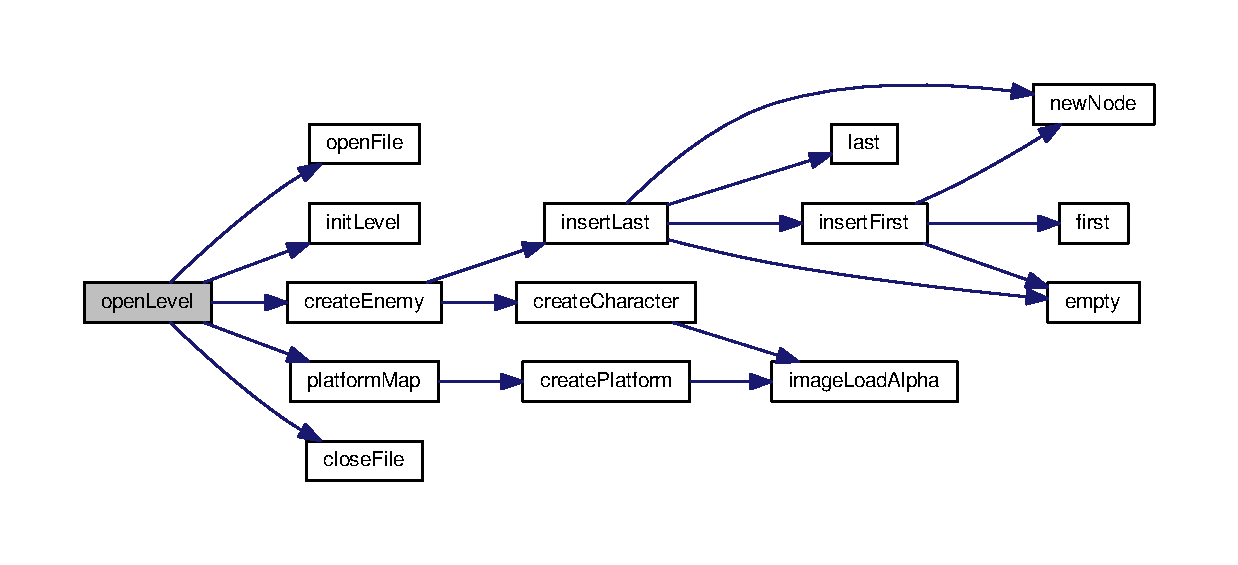
\includegraphics[width=350pt]{file__level_8c_a8464887031ce16d797b564fc7a9e661f_cgraph}
\end{center}
\end{figure}


\hypertarget{file__level_8c_a8f93e9edca6b3e54fa194e27bacf8f46}{\index{file\-\_\-level.\-c@{file\-\_\-level.\-c}!read\-Level\-File@{read\-Level\-File}}
\index{read\-Level\-File@{read\-Level\-File}!file_level.c@{file\-\_\-level.\-c}}
\paragraph[{read\-Level\-File}]{\setlength{\rightskip}{0pt plus 5cm}char $\ast$$\ast$ read\-Level\-File (
\begin{DoxyParamCaption}
\item[{char $\ast$}]{file\-\_\-path, }
\item[{int $\ast$}]{nb\-\_\-lvl}
\end{DoxyParamCaption}
)}}\label{file__level_8c_a8f93e9edca6b3e54fa194e27bacf8f46}
read a file level 
\begin{DoxyParams}[1]{Parameters}
\mbox{\tt out}  & {\em nb\-\_\-lvl} & number of level \\
\hline
\mbox{\tt out}  & {\em file\-\_\-path} & the file path \\
\hline
\end{DoxyParams}
\begin{DoxyReturn}{Returns}
pointer on the level list created 
\end{DoxyReturn}


Here is the call graph for this function\-:
\nopagebreak
\begin{figure}[H]
\begin{center}
\leavevmode
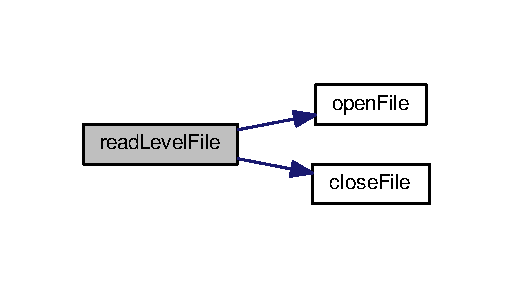
\includegraphics[width=246pt]{file__level_8c_a8f93e9edca6b3e54fa194e27bacf8f46_cgraph}
\end{center}
\end{figure}



\hypertarget{file__level_8h}{\subsection{file\-\_\-level.\-h File Reference}
\label{file__level_8h}\index{file\-\_\-level.\-h@{file\-\_\-level.\-h}}
}


\hyperlink{file__level_8c}{file\-\_\-level.\-c} header  


{\ttfamily \#include $<$stdio.\-h$>$}\\*
{\ttfamily \#include $<$stdlib.\-h$>$}\\*
{\ttfamily \#include $<$string.\-h$>$}\\*
{\ttfamily \#include \char`\"{}file.\-h\char`\"{}}\\*
{\ttfamily \#include \char`\"{}const.\-h\char`\"{}}\\*
{\ttfamily \#include \char`\"{}structures.\-h\char`\"{}}\\*
\subsubsection*{Macros}
\begin{DoxyCompactItemize}
\item 
\#define \hyperlink{file__level_8h_a6b20d41d6252e9871430c242cb1a56e7}{B\-U\-F\-F\-E\-R\-\_\-\-S\-I\-Z\-E}~2
\end{DoxyCompactItemize}
\subsubsection*{Functions}
\begin{DoxyCompactItemize}
\item 
\hyperlink{struct_level}{Level} $\ast$ \hyperlink{file__level_8h_a149f2e0878473ca6968717a39c119639}{open\-Level} (char $\ast$file\-\_\-name)
\item 
void \hyperlink{file__level_8h_a38020f30305d2344cdf39d06c7e8768e}{close\-Level} (\hyperlink{struct_level}{Level} $\ast$lvl)
\item 
\hyperlink{struct_level}{Level} $\ast$ \hyperlink{file__level_8h_a1749fb3f97d8b947c393f8eac9d29707}{init\-Level} (\hyperlink{struct_level}{Level} $\ast$lvl)
\item 
void \hyperlink{file__level_8h_aa22f94cc3689a4c98d553ff300c32bc9}{write\-Level} (char $\ast$file\-\_\-name, \hyperlink{struct_level}{Level} $\ast$lvl)
\item 
char $\ast$$\ast$ \hyperlink{file__level_8h_af646d7df8d540e24e2acc84fc3ea3ad3}{read\-Level\-File} (int $\ast$nb\-\_\-lvl)
\item 
void \hyperlink{file__level_8h_a3fafc12e3c322fc5a8166f7fb323bfe6}{close\-Level\-List} (char $\ast$$\ast$level\-\_\-names, int nb\-\_\-lvl)
\item 
\hyperlink{struct_level}{Level} $\ast$ \hyperlink{file__level_8h_a40c7ce420eb28ac24765fc244bd938ca}{adapt\-Size\-Level} (\hyperlink{struct_level}{Level} $\ast$lvl)
\item 
int \hyperlink{file__level_8h_abd4c02fab44779b57294a058c8486365}{search\-End\-Level} (\hyperlink{struct_level}{Level} $\ast$lvl)
\end{DoxyCompactItemize}


\subsubsection{Detailed Description}
\hyperlink{file__level_8c}{file\-\_\-level.\-c} header \begin{DoxyAuthor}{Author}
Remi B\-E\-R\-T\-H\-O, Glenn H\-E\-R\-R\-O\-U 
\end{DoxyAuthor}
\begin{DoxyDate}{Date}
2014-\/05-\/12 
\end{DoxyDate}
\begin{DoxyVersion}{Version}
2.\-0 
\end{DoxyVersion}


\subsubsection{Macro Definition Documentation}
\hypertarget{file__level_8h_a6b20d41d6252e9871430c242cb1a56e7}{\index{file\-\_\-level.\-h@{file\-\_\-level.\-h}!B\-U\-F\-F\-E\-R\-\_\-\-S\-I\-Z\-E@{B\-U\-F\-F\-E\-R\-\_\-\-S\-I\-Z\-E}}
\index{B\-U\-F\-F\-E\-R\-\_\-\-S\-I\-Z\-E@{B\-U\-F\-F\-E\-R\-\_\-\-S\-I\-Z\-E}!file_level.h@{file\-\_\-level.\-h}}
\paragraph[{B\-U\-F\-F\-E\-R\-\_\-\-S\-I\-Z\-E}]{\setlength{\rightskip}{0pt plus 5cm}\#define B\-U\-F\-F\-E\-R\-\_\-\-S\-I\-Z\-E~2}}\label{file__level_8h_a6b20d41d6252e9871430c242cb1a56e7}
The buffer size 

\subsubsection{Function Documentation}
\hypertarget{file__level_8h_a40c7ce420eb28ac24765fc244bd938ca}{\index{file\-\_\-level.\-h@{file\-\_\-level.\-h}!adapt\-Size\-Level@{adapt\-Size\-Level}}
\index{adapt\-Size\-Level@{adapt\-Size\-Level}!file_level.h@{file\-\_\-level.\-h}}
\paragraph[{adapt\-Size\-Level}]{\setlength{\rightskip}{0pt plus 5cm}{\bf Level}$\ast$ adapt\-Size\-Level (
\begin{DoxyParamCaption}
\item[{{\bf Level} $\ast$}]{lvl}
\end{DoxyParamCaption}
)}}\label{file__level_8h_a40c7ce420eb28ac24765fc244bd938ca}
Adapt the width of a level 
\begin{DoxyParams}[1]{Parameters}
\mbox{\tt in,out}  & {\em lvl} & the level to adapt \\
\hline
\end{DoxyParams}


Here is the call graph for this function\-:
\nopagebreak
\begin{figure}[H]
\begin{center}
\leavevmode
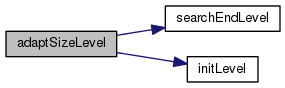
\includegraphics[width=286pt]{file__level_8h_a40c7ce420eb28ac24765fc244bd938ca_cgraph}
\end{center}
\end{figure}


\hypertarget{file__level_8h_a38020f30305d2344cdf39d06c7e8768e}{\index{file\-\_\-level.\-h@{file\-\_\-level.\-h}!close\-Level@{close\-Level}}
\index{close\-Level@{close\-Level}!file_level.h@{file\-\_\-level.\-h}}
\paragraph[{close\-Level}]{\setlength{\rightskip}{0pt plus 5cm}void close\-Level (
\begin{DoxyParamCaption}
\item[{{\bf Level} $\ast$}]{lvl}
\end{DoxyParamCaption}
)}}\label{file__level_8h_a38020f30305d2344cdf39d06c7e8768e}
Close a level by freeing its allocated memory 
\begin{DoxyParams}[1]{Parameters}
\mbox{\tt out}  & {\em lvl} & The level \\
\hline
\end{DoxyParams}
\hypertarget{file__level_8h_a3fafc12e3c322fc5a8166f7fb323bfe6}{\index{file\-\_\-level.\-h@{file\-\_\-level.\-h}!close\-Level\-List@{close\-Level\-List}}
\index{close\-Level\-List@{close\-Level\-List}!file_level.h@{file\-\_\-level.\-h}}
\paragraph[{close\-Level\-List}]{\setlength{\rightskip}{0pt plus 5cm}void close\-Level\-List (
\begin{DoxyParamCaption}
\item[{char $\ast$$\ast$}]{level\-\_\-names, }
\item[{int}]{nb\-\_\-lvl}
\end{DoxyParamCaption}
)}}\label{file__level_8h_a3fafc12e3c322fc5a8166f7fb323bfe6}
Free the array containing the list of the levels 
\begin{DoxyParams}[1]{Parameters}
\mbox{\tt in,out}  & {\em level\-\_\-names} & the list of existing levels \\
\hline
\mbox{\tt in}  & {\em nb\-\_\-lvl} & the number of existing levels \\
\hline
\end{DoxyParams}
\hypertarget{file__level_8h_a1749fb3f97d8b947c393f8eac9d29707}{\index{file\-\_\-level.\-h@{file\-\_\-level.\-h}!init\-Level@{init\-Level}}
\index{init\-Level@{init\-Level}!file_level.h@{file\-\_\-level.\-h}}
\paragraph[{init\-Level}]{\setlength{\rightskip}{0pt plus 5cm}{\bf Level}$\ast$ init\-Level (
\begin{DoxyParamCaption}
\item[{{\bf Level} $\ast$}]{lvl}
\end{DoxyParamCaption}
)}}\label{file__level_8h_a1749fb3f97d8b947c393f8eac9d29707}
Initialize a level. The width and the Height of the level must be stored in the level before calling this function. 
\begin{DoxyParams}[1]{Parameters}
\mbox{\tt out}  & {\em lvl} & The level \\
\hline
\end{DoxyParams}
\begin{DoxyReturn}{Returns}
a pointer on the level initialized 
\end{DoxyReturn}
\hypertarget{file__level_8h_a149f2e0878473ca6968717a39c119639}{\index{file\-\_\-level.\-h@{file\-\_\-level.\-h}!open\-Level@{open\-Level}}
\index{open\-Level@{open\-Level}!file_level.h@{file\-\_\-level.\-h}}
\paragraph[{open\-Level}]{\setlength{\rightskip}{0pt plus 5cm}{\bf Level}$\ast$ open\-Level (
\begin{DoxyParamCaption}
\item[{char $\ast$}]{file\-\_\-name}
\end{DoxyParamCaption}
)}}\label{file__level_8h_a149f2e0878473ca6968717a39c119639}
Open a level file and store the level corresponding to the file 
\begin{DoxyParams}[1]{Parameters}
\mbox{\tt in}  & {\em file\-\_\-name} & the name of the level file \\
\hline
\end{DoxyParams}
\begin{DoxyReturn}{Returns}
a pointer to the level created 
\end{DoxyReturn}


Here is the call graph for this function\-:
\nopagebreak
\begin{figure}[H]
\begin{center}
\leavevmode
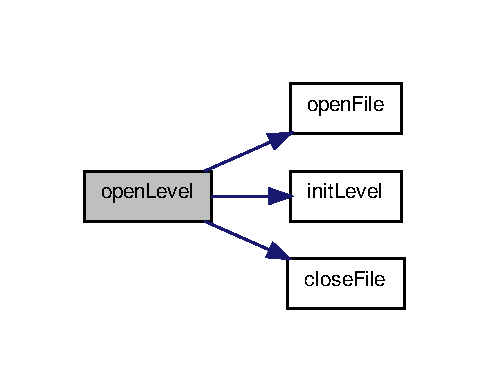
\includegraphics[width=234pt]{file__level_8h_a149f2e0878473ca6968717a39c119639_cgraph}
\end{center}
\end{figure}


\hypertarget{file__level_8h_af646d7df8d540e24e2acc84fc3ea3ad3}{\index{file\-\_\-level.\-h@{file\-\_\-level.\-h}!read\-Level\-File@{read\-Level\-File}}
\index{read\-Level\-File@{read\-Level\-File}!file_level.h@{file\-\_\-level.\-h}}
\paragraph[{read\-Level\-File}]{\setlength{\rightskip}{0pt plus 5cm}char$\ast$$\ast$ read\-Level\-File (
\begin{DoxyParamCaption}
\item[{int $\ast$}]{nb\-\_\-lvl}
\end{DoxyParamCaption}
)}}\label{file__level_8h_af646d7df8d540e24e2acc84fc3ea3ad3}
Read the file including the list of existing levels 
\begin{DoxyParams}[1]{Parameters}
\mbox{\tt out}  & {\em nb\-\_\-lvl} & the number of level in the file \\
\hline
\end{DoxyParams}
\begin{DoxyReturn}{Returns}
a pointer to an array of strings containing the list of the levels 
\end{DoxyReturn}


Here is the call graph for this function\-:
\nopagebreak
\begin{figure}[H]
\begin{center}
\leavevmode
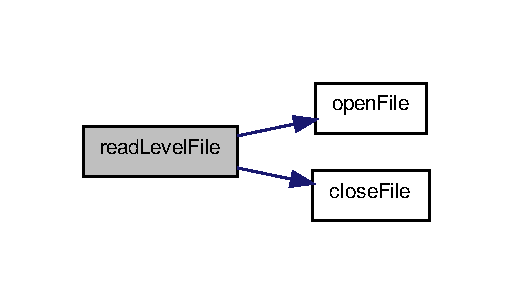
\includegraphics[width=246pt]{file__level_8h_af646d7df8d540e24e2acc84fc3ea3ad3_cgraph}
\end{center}
\end{figure}


\hypertarget{file__level_8h_abd4c02fab44779b57294a058c8486365}{\index{file\-\_\-level.\-h@{file\-\_\-level.\-h}!search\-End\-Level@{search\-End\-Level}}
\index{search\-End\-Level@{search\-End\-Level}!file_level.h@{file\-\_\-level.\-h}}
\paragraph[{search\-End\-Level}]{\setlength{\rightskip}{0pt plus 5cm}int search\-End\-Level (
\begin{DoxyParamCaption}
\item[{{\bf Level} $\ast$}]{lvl}
\end{DoxyParamCaption}
)}}\label{file__level_8h_abd4c02fab44779b57294a058c8486365}
Search the end of a level 
\begin{DoxyParams}[1]{Parameters}
\mbox{\tt in,out}  & {\em lvl} & the level \\
\hline
\end{DoxyParams}
\hypertarget{file__level_8h_aa22f94cc3689a4c98d553ff300c32bc9}{\index{file\-\_\-level.\-h@{file\-\_\-level.\-h}!write\-Level@{write\-Level}}
\index{write\-Level@{write\-Level}!file_level.h@{file\-\_\-level.\-h}}
\paragraph[{write\-Level}]{\setlength{\rightskip}{0pt plus 5cm}void write\-Level (
\begin{DoxyParamCaption}
\item[{char $\ast$}]{file\-\_\-name, }
\item[{{\bf Level} $\ast$}]{lvl}
\end{DoxyParamCaption}
)}}\label{file__level_8h_aa22f94cc3689a4c98d553ff300c32bc9}
Write the given level in the given file 
\begin{DoxyParams}[1]{Parameters}
\mbox{\tt in}  & {\em lvl} & the file \\
\hline
\mbox{\tt in}  & {\em file\-\_\-name} & the name of the file \\
\hline
\end{DoxyParams}


Here is the call graph for this function\-:
\nopagebreak
\begin{figure}[H]
\begin{center}
\leavevmode
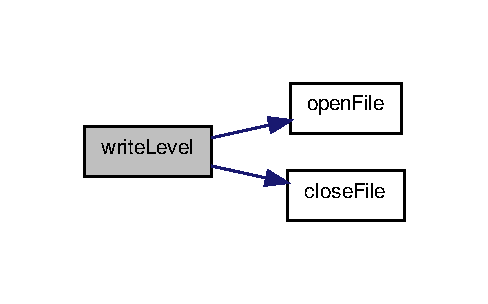
\includegraphics[width=350pt]{file__level_8h_aa22f94cc3689a4c98d553ff300c32bc9_cgraph}
\end{center}
\end{figure}



\hypertarget{game_8c}{\subsection{game.\-c File Reference}
\label{game_8c}\index{game.\-c@{game.\-c}}
}


Contain the main functions of the game.  


{\ttfamily \#include \char`\"{}game.\-h\char`\"{}}\\*
\subsubsection*{Functions}
\begin{DoxyCompactItemize}
\item 
void \hyperlink{game_8c_a3be984c6f3d228041d098485fe01f98c}{play} (S\-D\-L\-\_\-\-Surface $\ast$screen, char $\ast$level\-\_\-name, S\-D\-L\-Key $\ast$kc)
\item 
void \hyperlink{game_8c_aef36043913d82479cc03e51d01a320a1}{print\-Confirmation} (S\-D\-L\-\_\-\-Surface $\ast$screen, \hyperlink{struct_input}{Input} $\ast$in, int $\ast$go)
\end{DoxyCompactItemize}


\subsubsection{Detailed Description}
Contain the main functions of the game. \begin{DoxyAuthor}{Author}
Xavier C\-O\-P\-O\-N\-E\-T, Glenn H\-E\-R\-R\-O\-U 
\end{DoxyAuthor}
\begin{DoxyDate}{Date}
2014-\/05-\/15 
\end{DoxyDate}


\subsubsection{Function Documentation}
\hypertarget{game_8c_a3be984c6f3d228041d098485fe01f98c}{\index{game.\-c@{game.\-c}!play@{play}}
\index{play@{play}!game.c@{game.\-c}}
\paragraph[{play}]{\setlength{\rightskip}{0pt plus 5cm}void play (
\begin{DoxyParamCaption}
\item[{S\-D\-L\-\_\-\-Surface $\ast$}]{screen, }
\item[{char $\ast$}]{level\-\_\-name, }
\item[{S\-D\-L\-Key $\ast$}]{kc}
\end{DoxyParamCaption}
)}}\label{game_8c_a3be984c6f3d228041d098485fe01f98c}
Include the main loop of the game 
\begin{DoxyParams}[1]{Parameters}
\mbox{\tt in,out}  & {\em screen} & The screen of the game \\
\hline
\mbox{\tt in}  & {\em level\-\_\-name} & The name of the level \\
\hline
\mbox{\tt in}  & {\em kc} & The keyboard configuration \\
\hline
\end{DoxyParams}


Here is the call graph for this function\-:
\nopagebreak
\begin{figure}[H]
\begin{center}
\leavevmode
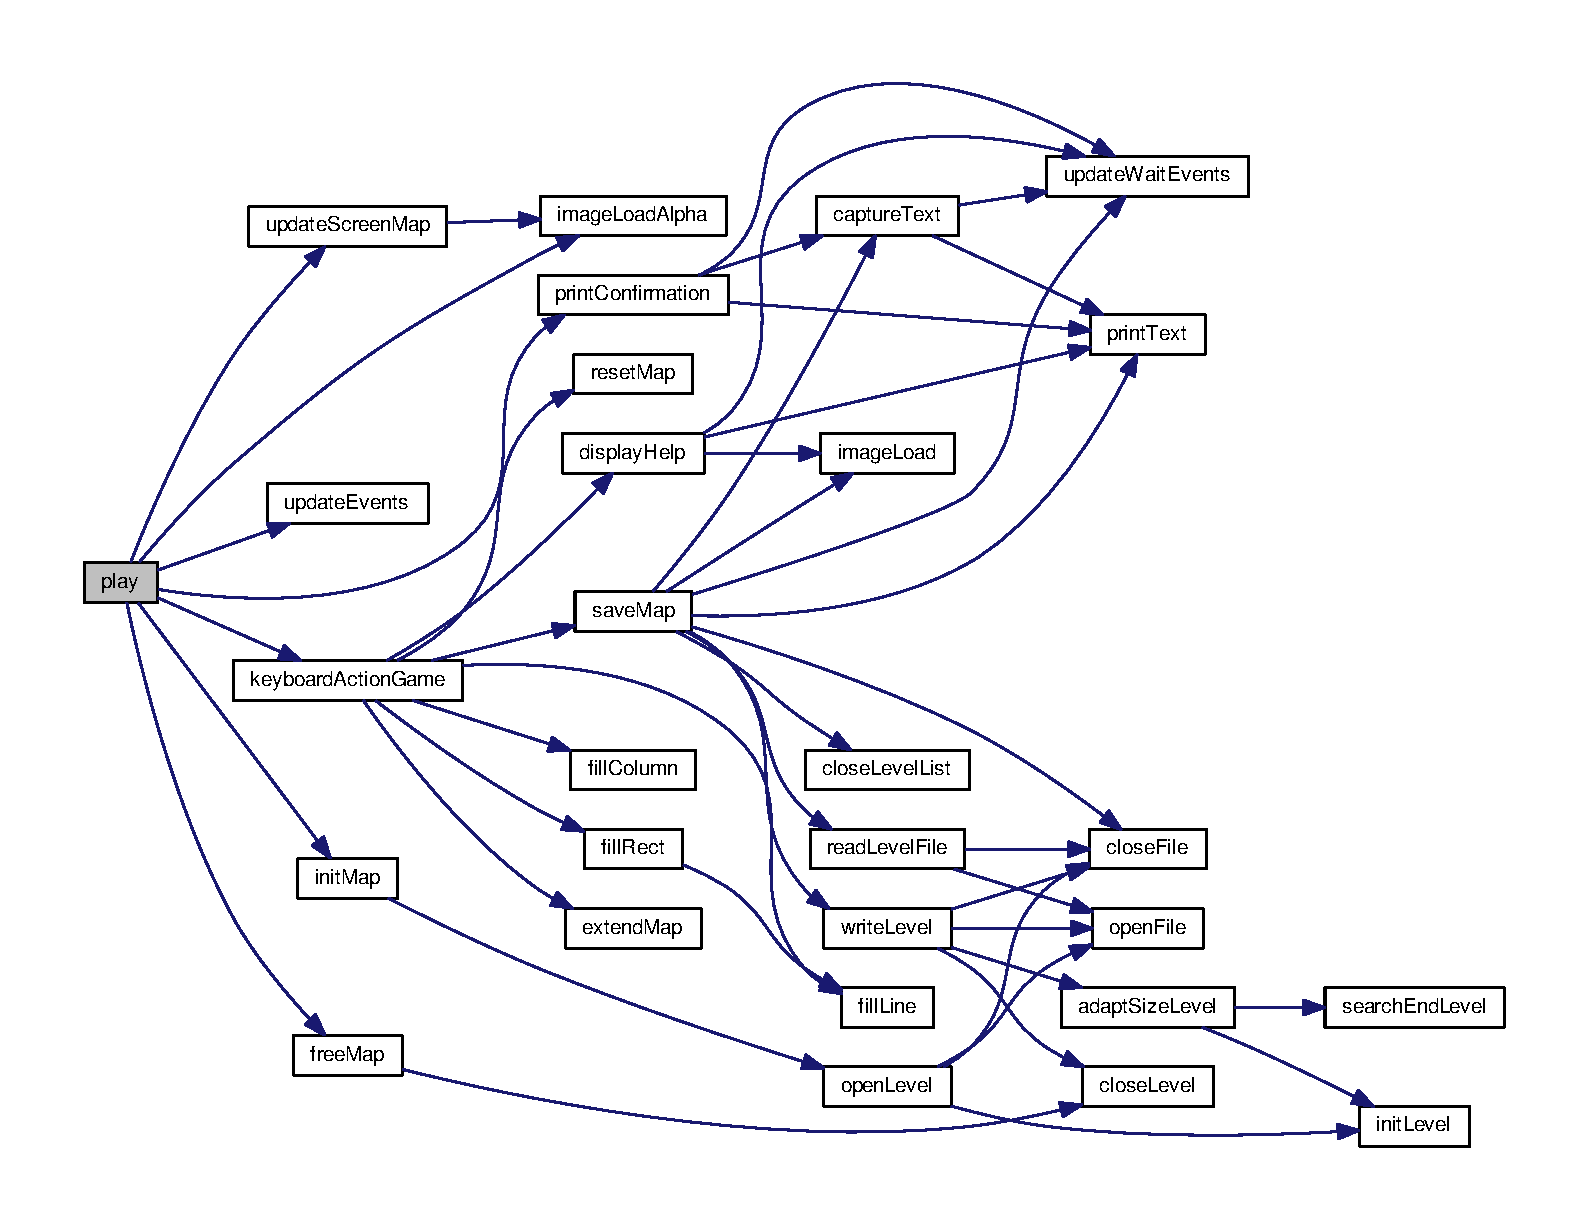
\includegraphics[width=350pt]{game_8c_a3be984c6f3d228041d098485fe01f98c_cgraph}
\end{center}
\end{figure}


\hypertarget{game_8c_aef36043913d82479cc03e51d01a320a1}{\index{game.\-c@{game.\-c}!print\-Confirmation@{print\-Confirmation}}
\index{print\-Confirmation@{print\-Confirmation}!game.c@{game.\-c}}
\paragraph[{print\-Confirmation}]{\setlength{\rightskip}{0pt plus 5cm}void print\-Confirmation (
\begin{DoxyParamCaption}
\item[{S\-D\-L\-\_\-\-Surface $\ast$}]{screen, }
\item[{{\bf Input} $\ast$}]{in, }
\item[{int $\ast$}]{go}
\end{DoxyParamCaption}
)}}\label{game_8c_aef36043913d82479cc03e51d01a320a1}
Display the confirmation screen, before leaving the edition of a level 
\begin{DoxyParams}[1]{Parameters}
\mbox{\tt out}  & {\em screen} & The screen of the game \\
\hline
\mbox{\tt in}  & {\em in} & The input structure \\
\hline
\mbox{\tt out}  & {\em go} & The main loop activation \\
\hline
\end{DoxyParams}


Here is the call graph for this function\-:
\nopagebreak
\begin{figure}[H]
\begin{center}
\leavevmode
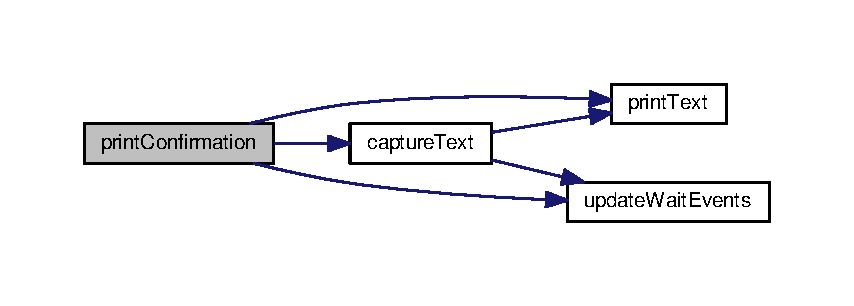
\includegraphics[width=350pt]{game_8c_aef36043913d82479cc03e51d01a320a1_cgraph}
\end{center}
\end{figure}



\hypertarget{game_8h}{\section{game.\-h File Reference}
\label{game_8h}\index{game.\-h@{game.\-h}}
}


Header of \hyperlink{game_8c}{game.\-c}.  


{\ttfamily \#include \char`\"{}const.\-h\char`\"{}}\\*
{\ttfamily \#include \char`\"{}file\-\_\-level.\-h\char`\"{}}\\*
{\ttfamily \#include \char`\"{}input.\-h\char`\"{}}\\*
{\ttfamily \#include \char`\"{}map.\-h\char`\"{}}\\*
Include dependency graph for game.\-h\-:\nopagebreak
\begin{figure}[H]
\begin{center}
\leavevmode
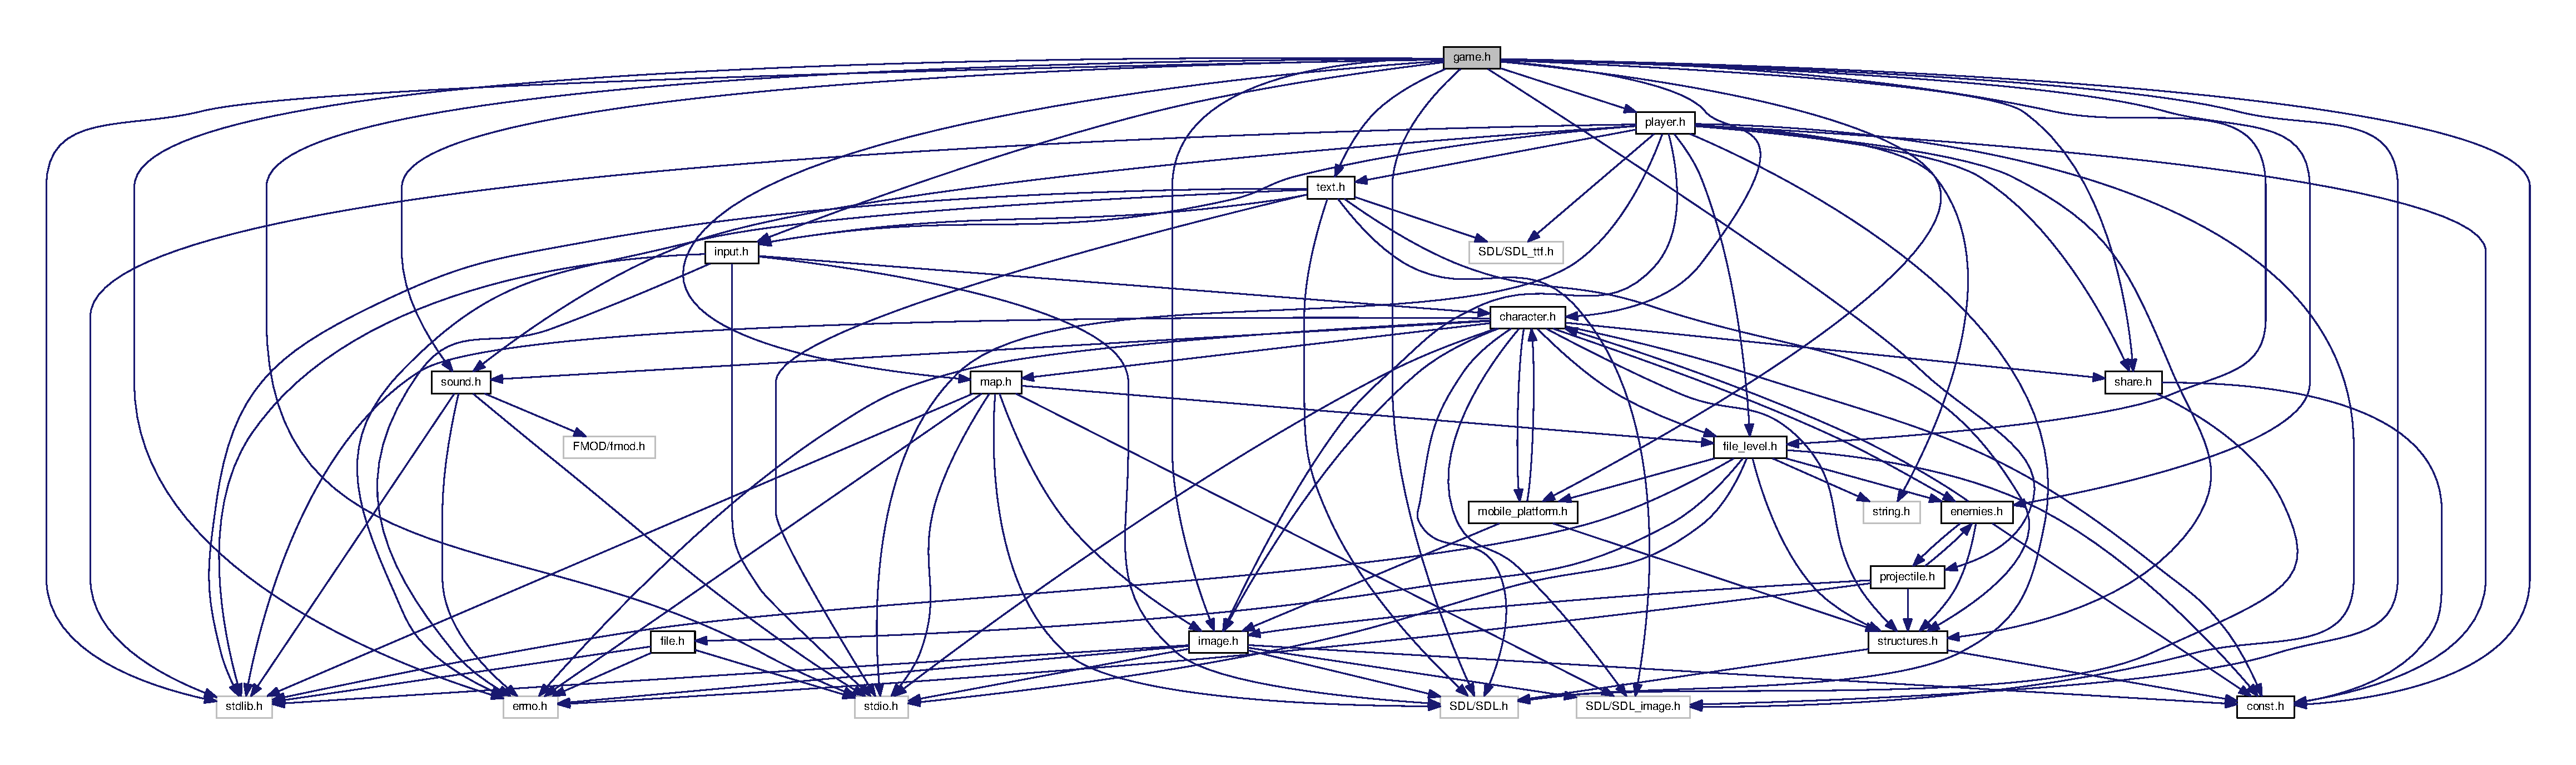
\includegraphics[width=350pt]{game_8h__incl}
\end{center}
\end{figure}
This graph shows which files directly or indirectly include this file\-:
\nopagebreak
\begin{figure}[H]
\begin{center}
\leavevmode
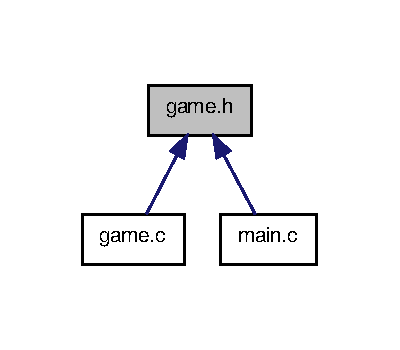
\includegraphics[width=254pt]{game_8h__dep__incl}
\end{center}
\end{figure}
\subsection*{Functions}
\begin{DoxyCompactItemize}
\item 
void \hyperlink{game_8h_ae342e4b762af0d52f4ee914643441426}{play} (S\-D\-L\-\_\-\-Surface $\ast$screen, char $\ast$level\-\_\-name)
\end{DoxyCompactItemize}


\subsection{Detailed Description}
Header of \hyperlink{game_8c}{game.\-c}. \begin{DoxyAuthor}{Author}
Xavier C\-O\-P\-O\-N\-E\-T, Glenn H\-E\-R\-R\-O\-U 
\end{DoxyAuthor}
\begin{DoxyDate}{Date}
2014-\/03-\/18 
\end{DoxyDate}


\subsection{Function Documentation}
\hypertarget{game_8h_ae342e4b762af0d52f4ee914643441426}{\index{game.\-h@{game.\-h}!play@{play}}
\index{play@{play}!game.h@{game.\-h}}
\subsubsection[{play}]{\setlength{\rightskip}{0pt plus 5cm}void play (
\begin{DoxyParamCaption}
\item[{S\-D\-L\-\_\-\-Surface $\ast$}]{screen, }
\item[{char $\ast$}]{level\-\_\-name}
\end{DoxyParamCaption}
)}}\label{game_8h_ae342e4b762af0d52f4ee914643441426}
Contains the infinite loop of the game, call the main functions 
\begin{DoxyParams}[1]{Parameters}
\mbox{\tt in,out}  & {\em screen} & Game screen \\
\hline
\mbox{\tt in}  & {\em level\-\_\-name} & \hyperlink{struct_level}{Level} name \\
\hline
\end{DoxyParams}


Here is the call graph for this function\-:
\nopagebreak
\begin{figure}[H]
\begin{center}
\leavevmode
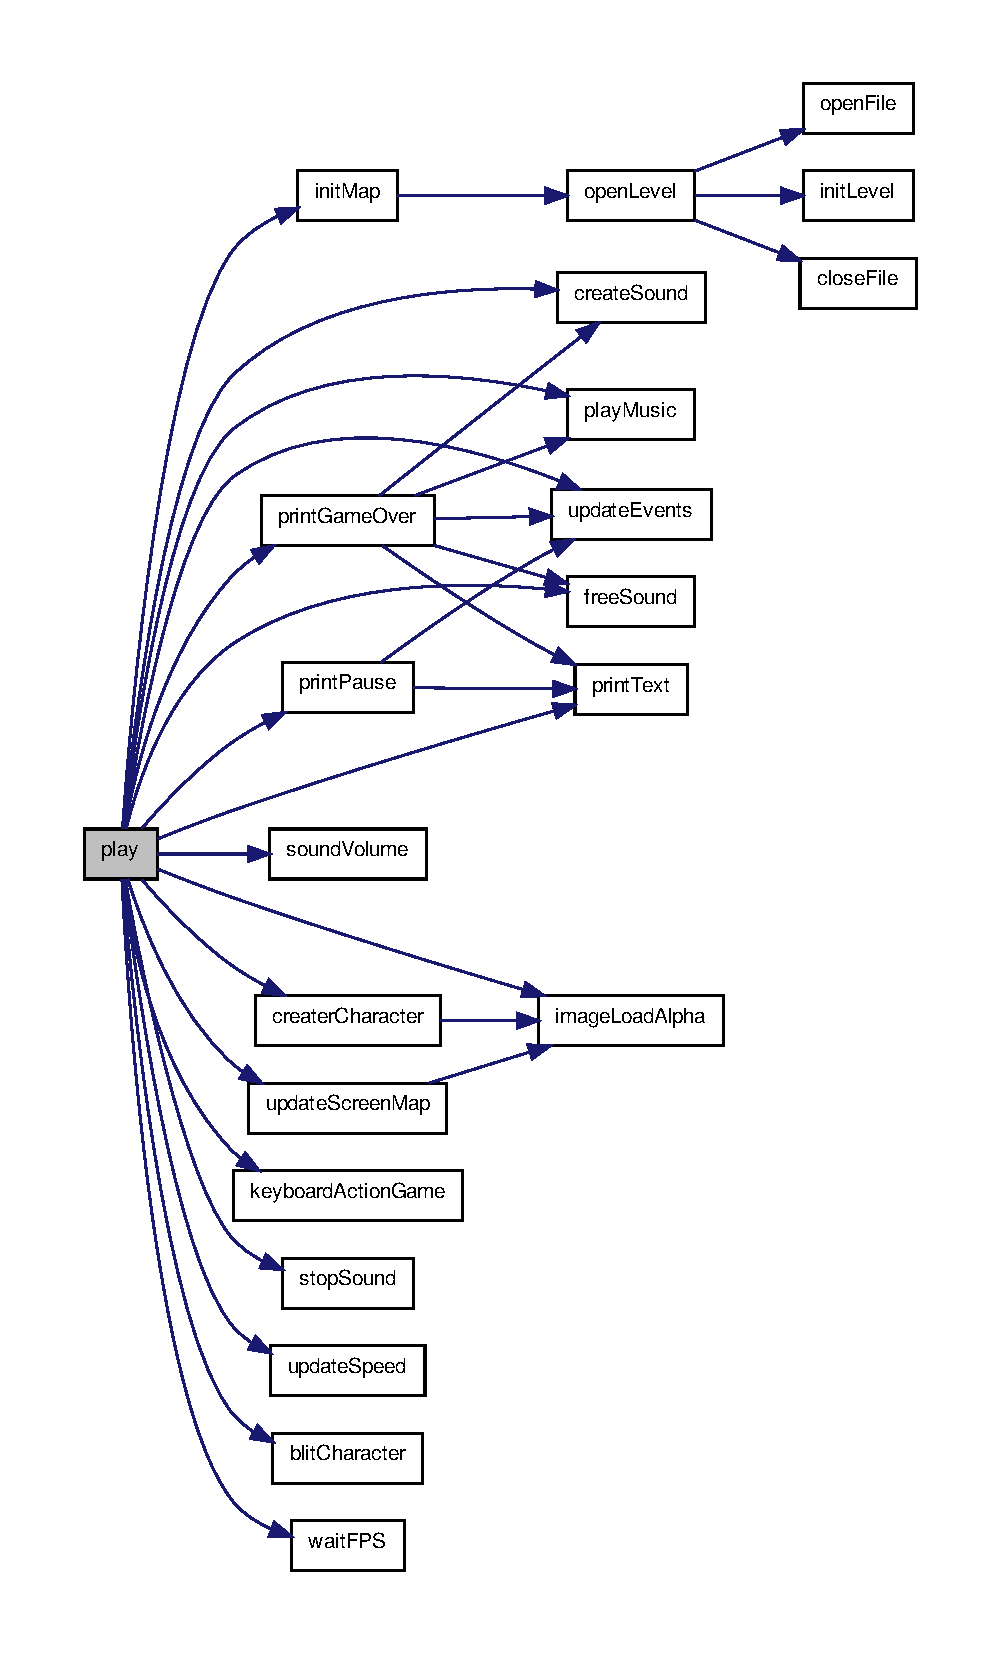
\includegraphics[width=306pt]{game_8h_ae342e4b762af0d52f4ee914643441426_cgraph}
\end{center}
\end{figure}



\hypertarget{image_8c}{\subsection{image.\-c File Reference}
\label{image_8c}\index{image.\-c@{image.\-c}}
}


Contain the functions managing the images.  


{\ttfamily \#include \char`\"{}image.\-h\char`\"{}}\\*
\subsubsection*{Functions}
\begin{DoxyCompactItemize}
\item 
S\-D\-L\-\_\-\-Surface $\ast$ \hyperlink{image_8c_a9862daea48ad8bfd1d3a0c401a9f5210}{image\-Load} (char $\ast$file\-\_\-name)
\item 
S\-D\-L\-\_\-\-Surface $\ast$ \hyperlink{image_8c_a569b068180b77bf2d44cf580322c68ad}{image\-Load\-Alpha} (char $\ast$file\-\_\-name)
\item 
void \hyperlink{image_8c_a3917cdd2e4b298f247aedfdf76268c75}{blit\-Color} (Uint32 red, Uint32 green, Uint32 blue, int alpha, S\-D\-L\-\_\-\-Surface $\ast$screen)
\end{DoxyCompactItemize}


\subsubsection{Detailed Description}
Contain the functions managing the images. \begin{DoxyAuthor}{Author}
Rémi B\-E\-R\-T\-H\-O 
\end{DoxyAuthor}
\begin{DoxyDate}{Date}
2014-\/02-\/27 
\end{DoxyDate}


\subsubsection{Function Documentation}
\hypertarget{image_8c_a3917cdd2e4b298f247aedfdf76268c75}{\index{image.\-c@{image.\-c}!blit\-Color@{blit\-Color}}
\index{blit\-Color@{blit\-Color}!image.c@{image.\-c}}
\paragraph[{blit\-Color}]{\setlength{\rightskip}{0pt plus 5cm}void blit\-Color (
\begin{DoxyParamCaption}
\item[{Uint32}]{red, }
\item[{Uint32}]{green, }
\item[{Uint32}]{blue, }
\item[{int}]{alpha, }
\item[{S\-D\-L\-\_\-\-Surface $\ast$}]{screen}
\end{DoxyParamCaption}
)}}\label{image_8c_a3917cdd2e4b298f247aedfdf76268c75}
Blit a color on the screen 
\begin{DoxyParams}[1]{Parameters}
\mbox{\tt in}  & {\em red} & the red of the color \\
\hline
\mbox{\tt in}  & {\em green} & the green of the color \\
\hline
\mbox{\tt in}  & {\em blue} & the blue of the color \\
\hline
\mbox{\tt in}  & {\em alpha} & the transparency of the image file \\
\hline
\mbox{\tt in}  & {\em screen} & the screen \\
\hline
\end{DoxyParams}
\hypertarget{image_8c_a9862daea48ad8bfd1d3a0c401a9f5210}{\index{image.\-c@{image.\-c}!image\-Load@{image\-Load}}
\index{image\-Load@{image\-Load}!image.c@{image.\-c}}
\paragraph[{image\-Load}]{\setlength{\rightskip}{0pt plus 5cm}S\-D\-L\-\_\-\-Surface $\ast$ image\-Load (
\begin{DoxyParamCaption}
\item[{char $\ast$}]{file\-\_\-name}
\end{DoxyParamCaption}
)}}\label{image_8c_a9862daea48ad8bfd1d3a0c401a9f5210}
Load an image 
\begin{DoxyParams}[1]{Parameters}
\mbox{\tt in}  & {\em file\-\_\-name} & the name of the image file \\
\hline
\end{DoxyParams}
\begin{DoxyReturn}{Returns}
a pointer on the S\-D\-L\-\_\-\-Surface created 
\end{DoxyReturn}
\hypertarget{image_8c_a569b068180b77bf2d44cf580322c68ad}{\index{image.\-c@{image.\-c}!image\-Load\-Alpha@{image\-Load\-Alpha}}
\index{image\-Load\-Alpha@{image\-Load\-Alpha}!image.c@{image.\-c}}
\paragraph[{image\-Load\-Alpha}]{\setlength{\rightskip}{0pt plus 5cm}S\-D\-L\-\_\-\-Surface $\ast$ image\-Load\-Alpha (
\begin{DoxyParamCaption}
\item[{char $\ast$}]{file\-\_\-name}
\end{DoxyParamCaption}
)}}\label{image_8c_a569b068180b77bf2d44cf580322c68ad}
Load an image with alpha management 
\begin{DoxyParams}[1]{Parameters}
\mbox{\tt in}  & {\em file\-\_\-name} & the name of the image file \\
\hline
\end{DoxyParams}
\begin{DoxyReturn}{Returns}
a pointer on the S\-D\-L\-\_\-\-Surface created 
\end{DoxyReturn}

\hypertarget{image_8h}{\subsection{image.\-h File Reference}
\label{image_8h}\index{image.\-h@{image.\-h}}
}


contient les fonction liées aux images  


{\ttfamily \#include $<$stdlib.\-h$>$}\\*
{\ttfamily \#include $<$stdio.\-h$>$}\\*
{\ttfamily \#include $<$errno.\-h$>$}\\*
{\ttfamily \#include $<$S\-D\-L/\-S\-D\-L.\-h$>$}\\*
{\ttfamily \#include $<$S\-D\-L/\-S\-D\-L\-\_\-image.\-h$>$}\\*
{\ttfamily \#include \char`\"{}const.\-h\char`\"{}}\\*
\subsubsection*{Functions}
\begin{DoxyCompactItemize}
\item 
S\-D\-L\-\_\-\-Surface $\ast$ \hyperlink{image_8h_aa53e98f2ff3d527d25b36023ea7f9d56}{image\-Load} (char $\ast$file\-\_\-name)
\item 
S\-D\-L\-\_\-\-Surface $\ast$ \hyperlink{image_8h_a469cf40e18cf579993e349b4393a2876}{image\-Load\-Alpha} (char $\ast$file\-\_\-name)
\item 
void \hyperlink{image_8h_a3917cdd2e4b298f247aedfdf76268c75}{blit\-Color} (Uint32 red, Uint32 green, Uint32 blue, int alpha, S\-D\-L\-\_\-\-Surface $\ast$screen)
\end{DoxyCompactItemize}


\subsubsection{Detailed Description}
contient les fonction liées aux images \begin{DoxyAuthor}{Author}
Rémi B\-E\-R\-T\-H\-O 
\end{DoxyAuthor}
\begin{DoxyDate}{Date}
2014-\/02-\/27 
\end{DoxyDate}


\subsubsection{Function Documentation}
\hypertarget{image_8h_a3917cdd2e4b298f247aedfdf76268c75}{\index{image.\-h@{image.\-h}!blit\-Color@{blit\-Color}}
\index{blit\-Color@{blit\-Color}!image.h@{image.\-h}}
\paragraph[{blit\-Color}]{\setlength{\rightskip}{0pt plus 5cm}void blit\-Color (
\begin{DoxyParamCaption}
\item[{Uint32}]{red, }
\item[{Uint32}]{green, }
\item[{Uint32}]{blue, }
\item[{int}]{alpha, }
\item[{S\-D\-L\-\_\-\-Surface $\ast$}]{screen}
\end{DoxyParamCaption}
)}}\label{image_8h_a3917cdd2e4b298f247aedfdf76268c75}
Blit a color on the screen 
\begin{DoxyParams}[1]{Parameters}
\mbox{\tt in}  & {\em red} & the red of the color \\
\hline
\mbox{\tt in}  & {\em green} & the green of the color \\
\hline
\mbox{\tt in}  & {\em blue} & the blue of the color \\
\hline
\mbox{\tt in}  & {\em alpha} & the transparency of the image file \\
\hline
\mbox{\tt in}  & {\em screen} & the screen \\
\hline
\end{DoxyParams}
\hypertarget{image_8h_aa53e98f2ff3d527d25b36023ea7f9d56}{\index{image.\-h@{image.\-h}!image\-Load@{image\-Load}}
\index{image\-Load@{image\-Load}!image.h@{image.\-h}}
\paragraph[{image\-Load}]{\setlength{\rightskip}{0pt plus 5cm}S\-D\-L\-\_\-\-Surface$\ast$ image\-Load (
\begin{DoxyParamCaption}
\item[{char $\ast$}]{file\-\_\-name}
\end{DoxyParamCaption}
)}}\label{image_8h_aa53e98f2ff3d527d25b36023ea7f9d56}
Load an image 
\begin{DoxyParams}[1]{Parameters}
\mbox{\tt in}  & {\em file\-\_\-name} & the name of the image file \\
\hline
\end{DoxyParams}
\begin{DoxyReturn}{Returns}
a pointer on the S\-D\-L\-\_\-\-Surface created 
\end{DoxyReturn}
\hypertarget{image_8h_a469cf40e18cf579993e349b4393a2876}{\index{image.\-h@{image.\-h}!image\-Load\-Alpha@{image\-Load\-Alpha}}
\index{image\-Load\-Alpha@{image\-Load\-Alpha}!image.h@{image.\-h}}
\paragraph[{image\-Load\-Alpha}]{\setlength{\rightskip}{0pt plus 5cm}S\-D\-L\-\_\-\-Surface$\ast$ image\-Load\-Alpha (
\begin{DoxyParamCaption}
\item[{char $\ast$}]{file\-\_\-name}
\end{DoxyParamCaption}
)}}\label{image_8h_a469cf40e18cf579993e349b4393a2876}
Load an image with alpha management 
\begin{DoxyParams}[1]{Parameters}
\mbox{\tt in}  & {\em file\-\_\-name} & the name of the image file \\
\hline
\end{DoxyParams}
\begin{DoxyReturn}{Returns}
a pointer on the S\-D\-L\-\_\-\-Surface created 
\end{DoxyReturn}

\hypertarget{input_8c}{\subsection{input.\-c File Reference}
\label{input_8c}\index{input.\-c@{input.\-c}}
}
{\ttfamily \#include \char`\"{}input.\-h\char`\"{}}\\*
\subsubsection*{Functions}
\begin{DoxyCompactItemize}
\item 
void \hyperlink{input_8c_a907831170dedec3a0af4e4b1e178b854}{update\-Events} (\hyperlink{struct_input}{Input} $\ast$in)
\item 
void \hyperlink{input_8c_a0f2aa7e2cd7674e43532893e4f2802e8}{keyboard\-Action\-Game} (S\-D\-L\-\_\-\-Surface $\ast$screen, \hyperlink{struct_input}{Input} $\ast$in, \hyperlink{struct_map}{Map} $\ast$m, \hyperlink{struct_cursor}{Cursor} $\ast$cursor, S\-D\-L\-Key $\ast$kc)
\item 
int \hyperlink{input_8c_ad3310b398fa046500863c183fd4468e6}{update\-Wait\-Events} (\hyperlink{struct_input}{Input} $\ast$in)
\item 
int \hyperlink{input_8c_aac9044909637f02a277d101651e126a7}{keyboard\-Action\-Menu} (\hyperlink{struct_input}{Input} $\ast$in, int $\ast$cursor\-Pos, int $\ast$select, int nb\-\_\-options)
\end{DoxyCompactItemize}


\subsubsection{Detailed Description}
\begin{DoxyAuthor}{Author}
Xavier C\-O\-P\-O\-N\-E\-T, Glenn H\-E\-R\-R\-O\-U 
\end{DoxyAuthor}
\begin{DoxyDate}{Date}
2014-\/03-\/18 
\end{DoxyDate}


\subsubsection{Function Documentation}
\hypertarget{input_8c_a0f2aa7e2cd7674e43532893e4f2802e8}{\index{input.\-c@{input.\-c}!keyboard\-Action\-Game@{keyboard\-Action\-Game}}
\index{keyboard\-Action\-Game@{keyboard\-Action\-Game}!input.c@{input.\-c}}
\paragraph[{keyboard\-Action\-Game}]{\setlength{\rightskip}{0pt plus 5cm}void keyboard\-Action\-Game (
\begin{DoxyParamCaption}
\item[{S\-D\-L\-\_\-\-Surface $\ast$}]{screen, }
\item[{{\bf Input} $\ast$}]{in, }
\item[{{\bf Map} $\ast$}]{m, }
\item[{{\bf Cursor} $\ast$}]{cursor, }
\item[{S\-D\-L\-Key $\ast$}]{kc}
\end{DoxyParamCaption}
)}}\label{input_8c_a0f2aa7e2cd7674e43532893e4f2802e8}
perform action commanded by keyboard action 
\begin{DoxyParams}[1]{Parameters}
\mbox{\tt in,out}  & {\em screen} & The screen of the game \\
\hline
\mbox{\tt in,out}  & {\em in} & the input structure \\
\hline
\mbox{\tt in,out}  & {\em m} & the map to update \\
\hline
\mbox{\tt in,out}  & {\em cursor} & the cursor structure \\
\hline
\mbox{\tt in}  & {\em kc} & the keyboard bindings \\
\hline
\end{DoxyParams}


Here is the call graph for this function\-:
\nopagebreak
\begin{figure}[H]
\begin{center}
\leavevmode
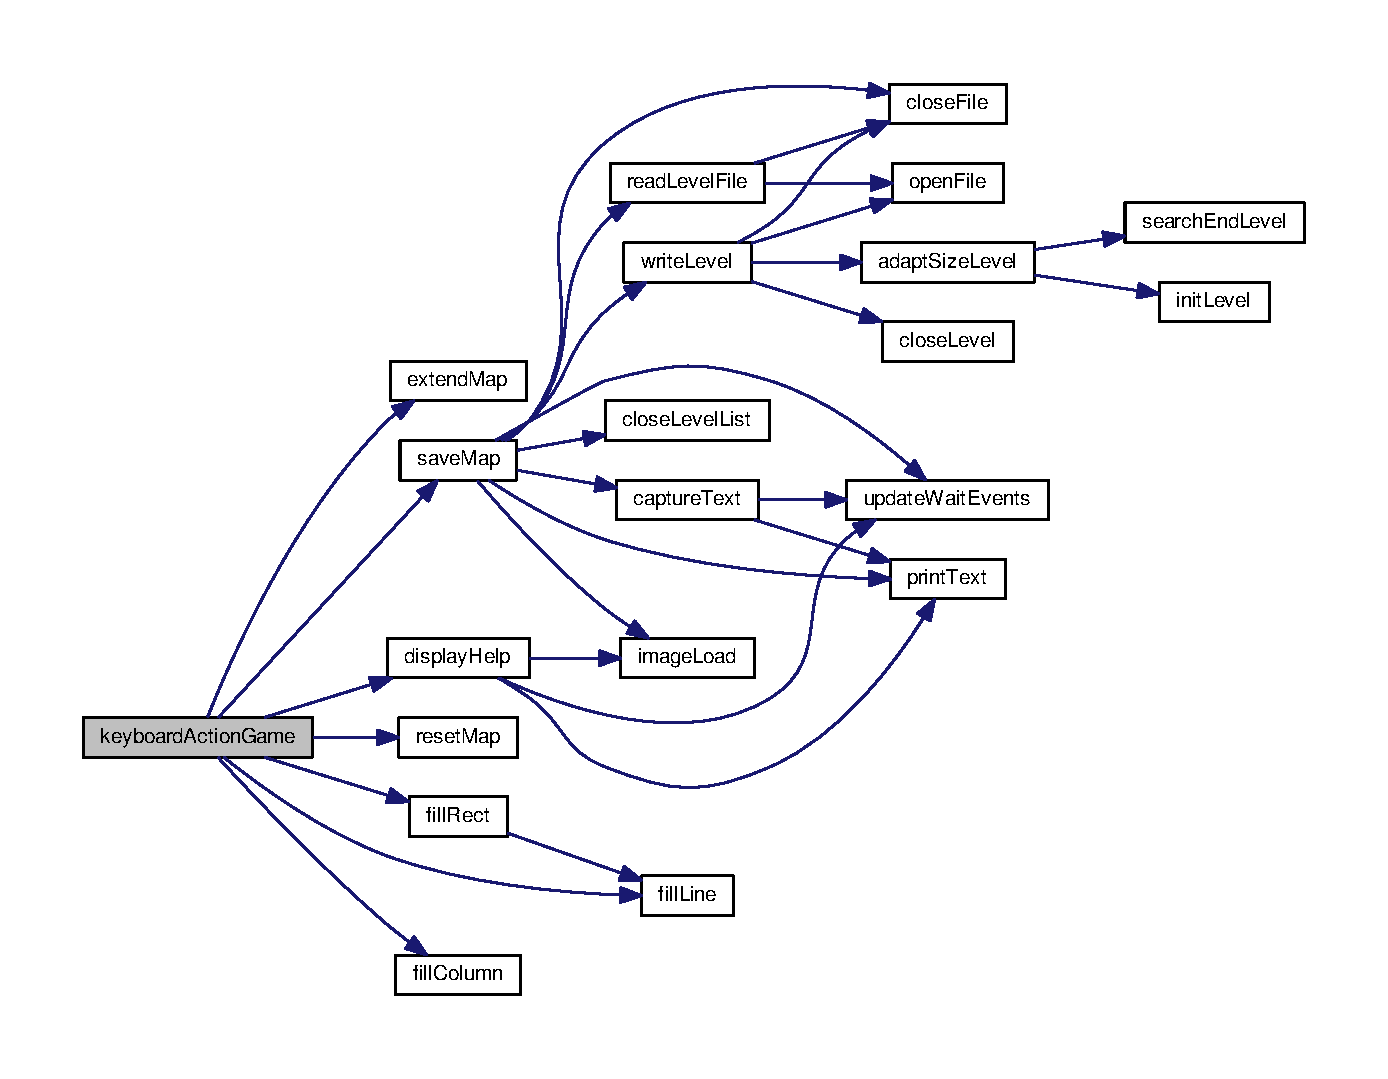
\includegraphics[width=350pt]{input_8c_a0f2aa7e2cd7674e43532893e4f2802e8_cgraph}
\end{center}
\end{figure}


\hypertarget{input_8c_aac9044909637f02a277d101651e126a7}{\index{input.\-c@{input.\-c}!keyboard\-Action\-Menu@{keyboard\-Action\-Menu}}
\index{keyboard\-Action\-Menu@{keyboard\-Action\-Menu}!input.c@{input.\-c}}
\paragraph[{keyboard\-Action\-Menu}]{\setlength{\rightskip}{0pt plus 5cm}void keyboard\-Action\-Menu (
\begin{DoxyParamCaption}
\item[{{\bf Input} $\ast$}]{in, }
\item[{int $\ast$}]{cursor\-Pos, }
\item[{int $\ast$}]{select, }
\item[{int}]{nb\-\_\-options}
\end{DoxyParamCaption}
)}}\label{input_8c_aac9044909637f02a277d101651e126a7}
perform menu action commanded by keyboard action 
\begin{DoxyParams}[1]{Parameters}
\mbox{\tt in}  & {\em in} & the input structure \\
\hline
\mbox{\tt out}  & {\em cursor\-Pos} & the cursor position \\
\hline
\mbox{\tt out}  & {\em select} & boolean about selecting the option or quit to title screen \\
\hline
\mbox{\tt in}  & {\em nb\-\_\-options} & the number of options of the menu \\
\hline
\end{DoxyParams}
\hypertarget{input_8c_a907831170dedec3a0af4e4b1e178b854}{\index{input.\-c@{input.\-c}!update\-Events@{update\-Events}}
\index{update\-Events@{update\-Events}!input.c@{input.\-c}}
\paragraph[{update\-Events}]{\setlength{\rightskip}{0pt plus 5cm}void update\-Events (
\begin{DoxyParamCaption}
\item[{{\bf Input} $\ast$}]{in}
\end{DoxyParamCaption}
)}}\label{input_8c_a907831170dedec3a0af4e4b1e178b854}
get keyboard input with a S\-D\-L\-\_\-\-Poll\-Event 
\begin{DoxyParams}[1]{Parameters}
\mbox{\tt out}  & {\em in} & the input structure \\
\hline
\end{DoxyParams}
\hypertarget{input_8c_ad3310b398fa046500863c183fd4468e6}{\index{input.\-c@{input.\-c}!update\-Wait\-Events@{update\-Wait\-Events}}
\index{update\-Wait\-Events@{update\-Wait\-Events}!input.c@{input.\-c}}
\paragraph[{update\-Wait\-Events}]{\setlength{\rightskip}{0pt plus 5cm}int update\-Wait\-Events (
\begin{DoxyParamCaption}
\item[{{\bf Input} $\ast$}]{in}
\end{DoxyParamCaption}
)}}\label{input_8c_ad3310b398fa046500863c183fd4468e6}
get keyboard input with a S\-D\-L\-\_\-\-Wait\-Event 
\begin{DoxyParams}[1]{Parameters}
\mbox{\tt out}  & {\em in} & the input structure \\
\hline
\end{DoxyParams}
\begin{DoxyReturn}{Returns}
1 if a key is activated 
\end{DoxyReturn}

\hypertarget{main_8c}{\subsection{main.\-c File Reference}
\label{main_8c}\index{main.\-c@{main.\-c}}
}
{\ttfamily \#include \char`\"{}game.\-h\char`\"{}}\\*
{\ttfamily \#include \char`\"{}const.\-h\char`\"{}}\\*
{\ttfamily \#include \char`\"{}menu.\-h\char`\"{}}\\*
{\ttfamily \#include \char`\"{}menu\-\_\-level.\-h\char`\"{}}\\*
{\ttfamily \#include \char`\"{}menu\-\_\-option.\-h\char`\"{}}\\*
{\ttfamily \#include \char`\"{}option.\-h\char`\"{}}\\*
\subsubsection*{Functions}
\begin{DoxyCompactItemize}
\item 
int \hyperlink{main_8c_a0ddf1224851353fc92bfbff6f499fa97}{main} (int argc, char $\ast$argv\mbox{[}$\,$\mbox{]})
\end{DoxyCompactItemize}


\subsubsection{Detailed Description}
\begin{DoxyAuthor}{Author}
Xavier C\-O\-P\-O\-N\-E\-T 
\end{DoxyAuthor}
\begin{DoxyDate}{Date}
2014-\/02-\/27 
\end{DoxyDate}


\subsubsection{Function Documentation}
\hypertarget{main_8c_a0ddf1224851353fc92bfbff6f499fa97}{\index{main.\-c@{main.\-c}!main@{main}}
\index{main@{main}!main.c@{main.\-c}}
\paragraph[{main}]{\setlength{\rightskip}{0pt plus 5cm}int main (
\begin{DoxyParamCaption}
\item[{int}]{argc, }
\item[{char $\ast$}]{argv\mbox{[}$\,$\mbox{]}}
\end{DoxyParamCaption}
)}}\label{main_8c_a0ddf1224851353fc92bfbff6f499fa97}
Main 
\begin{DoxyParams}[1]{Parameters}
\mbox{\tt in,out}  & {\em argc} & argc \\
\hline
\mbox{\tt in,out}  & {\em argv} & argv \\
\hline
\end{DoxyParams}


Here is the call graph for this function\-:
\nopagebreak
\begin{figure}[H]
\begin{center}
\leavevmode
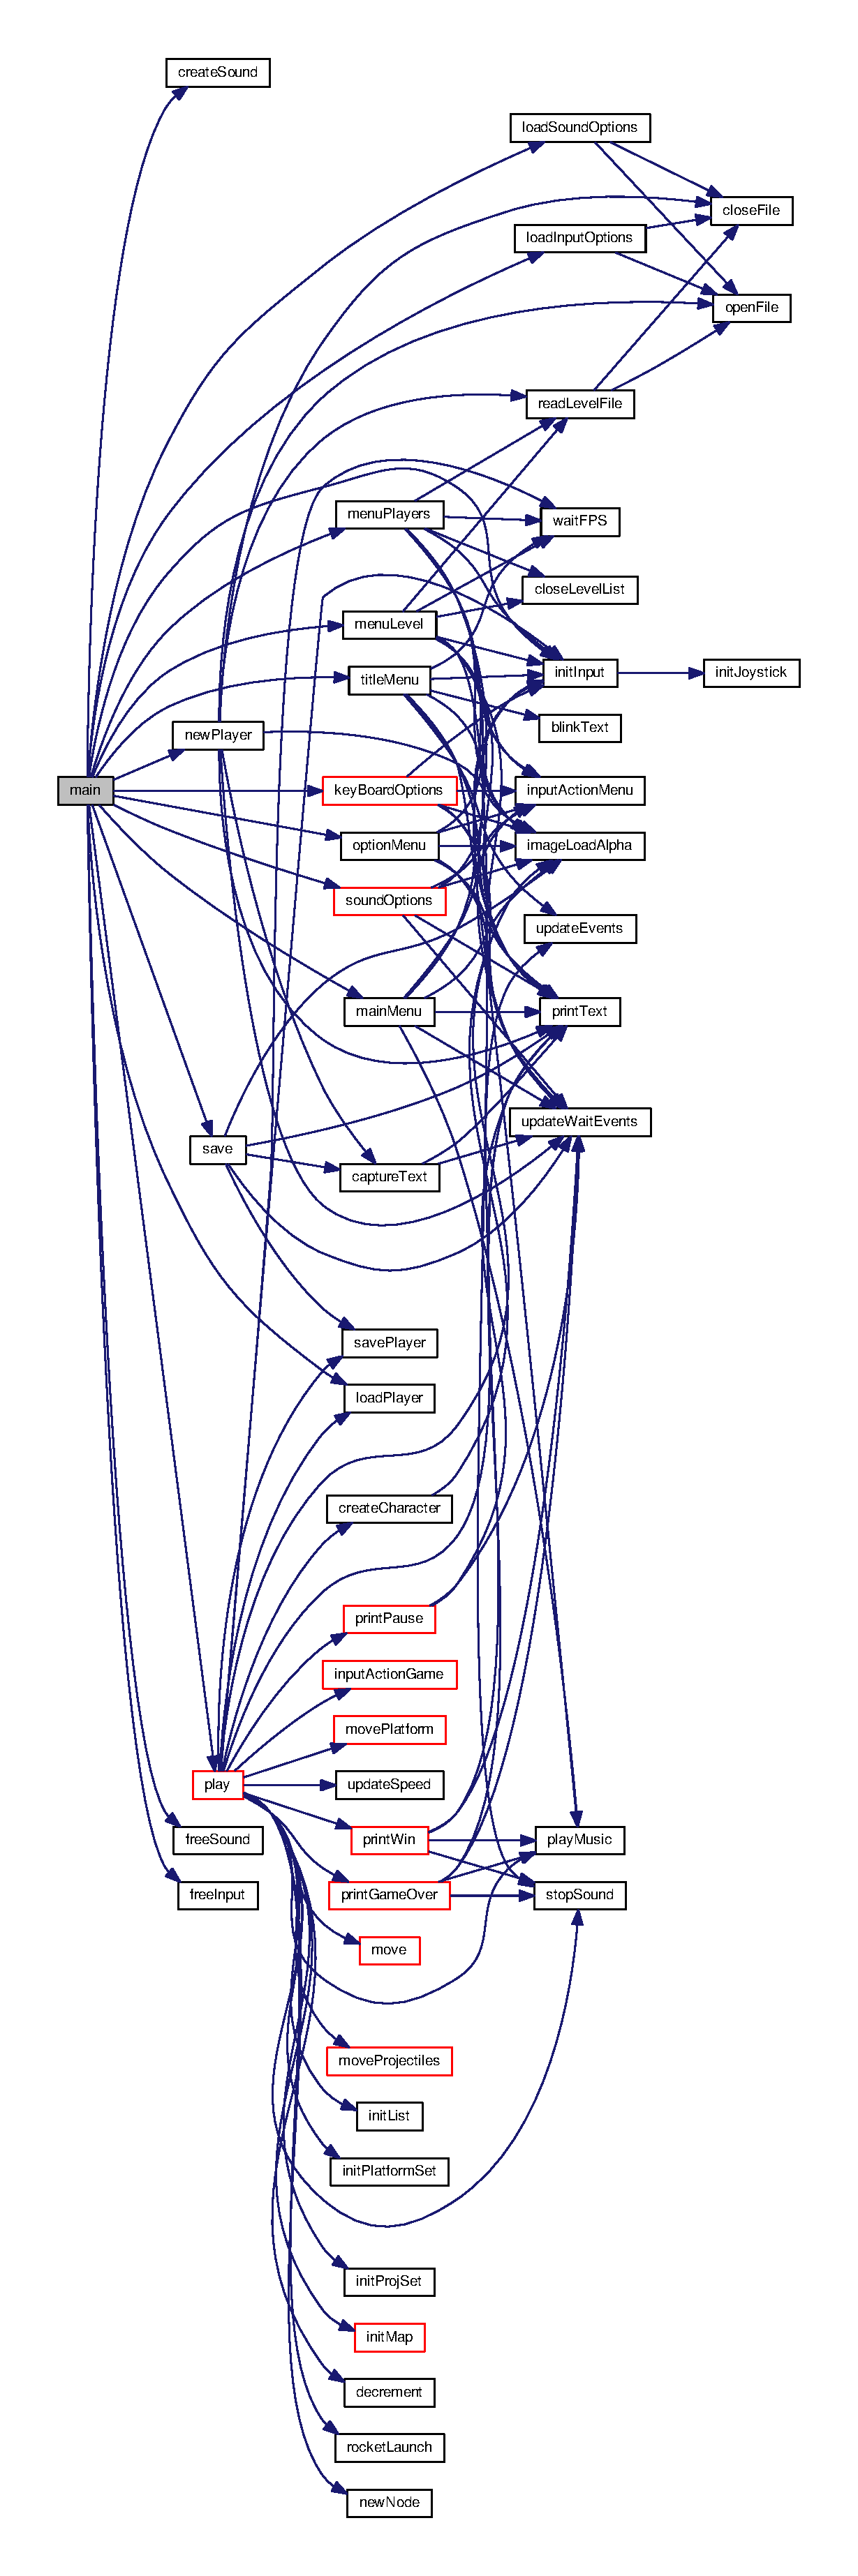
\includegraphics[width=350pt]{main_8c_a0ddf1224851353fc92bfbff6f499fa97_cgraph}
\end{center}
\end{figure}



\hypertarget{map_8c}{\subsection{map.\-c File Reference}
\label{map_8c}\index{map.\-c@{map.\-c}}
}


loading and displaying the map  


{\ttfamily \#include \char`\"{}map.\-h\char`\"{}}\\*
\subsubsection*{Functions}
\begin{DoxyCompactItemize}
\item 
void \hyperlink{map_8c_afc8482e2afe6f96b7d6cb6ce3fc7081c}{update\-Screen\-Map} (S\-D\-L\-\_\-\-Surface $\ast$screen, \hyperlink{struct_map}{Map} $\ast$m, char $\ast$tileset)
\item 
void \hyperlink{map_8c_a6f031e5ad35ada9038d3a72a56053760}{scrolling} (\hyperlink{struct_map}{Map} $\ast$m, int direction, float speed)
\item 
\hyperlink{struct_map}{Map} $\ast$ \hyperlink{map_8c_ace46be3df708e41a326676e6ad122bcc}{init\-Map} (S\-D\-L\-\_\-\-Surface $\ast$screen, char $\ast$level\-\_\-name, \hyperlink{structlist}{list} $\ast$l, \hyperlink{structplatform_set}{platform\-Set} $\ast$ps)
\item 
void \hyperlink{map_8c_ac8d4dd6fc80c79d9cb5899684740d074}{free\-Map} (\hyperlink{struct_map}{Map} $\ast$m)
\item 
int \hyperlink{map_8c_abf181167fafe365865bf0468959f1426}{collision\-Map} (S\-D\-L\-\_\-\-Rect r, \hyperlink{struct_map}{Map} $\ast$m, int type)
\end{DoxyCompactItemize}


\subsubsection{Detailed Description}
loading and displaying the map \begin{DoxyAuthor}{Author}
Xavier C\-O\-P\-O\-N\-E\-T 
\end{DoxyAuthor}
\begin{DoxyDate}{Date}
2014-\/03-\/18 
\end{DoxyDate}


\subsubsection{Function Documentation}
\hypertarget{map_8c_abf181167fafe365865bf0468959f1426}{\index{map.\-c@{map.\-c}!collision\-Map@{collision\-Map}}
\index{collision\-Map@{collision\-Map}!map.c@{map.\-c}}
\paragraph[{collision\-Map}]{\setlength{\rightskip}{0pt plus 5cm}int collision\-Map (
\begin{DoxyParamCaption}
\item[{S\-D\-L\-\_\-\-Rect}]{r, }
\item[{{\bf Map} $\ast$}]{m, }
\item[{int}]{type}
\end{DoxyParamCaption}
)}}\label{map_8c_abf181167fafe365865bf0468959f1426}
determine if there is a collision beteewen a sprite and a \char`\"{}wall\char`\"{} of the map 
\begin{DoxyParams}[1]{Parameters}
\mbox{\tt in}  & {\em r} & S\-D\-L\-\_\-\-Rect corresponding to the sprite \\
\hline
\mbox{\tt in}  & {\em m} & map \\
\hline
\mbox{\tt in}  & {\em type} & 0 if not a projectile \\
\hline
\end{DoxyParams}
\begin{DoxyReturn}{Returns}
1 if there is a collision, 0 if not,2 if collision with star/coin, 3 if spring 
\end{DoxyReturn}


Here is the call graph for this function\-:\nopagebreak
\begin{figure}[H]
\begin{center}
\leavevmode
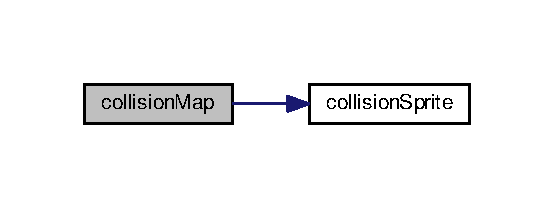
\includegraphics[width=266pt]{map_8c_abf181167fafe365865bf0468959f1426_cgraph}
\end{center}
\end{figure}


\hypertarget{map_8c_ac8d4dd6fc80c79d9cb5899684740d074}{\index{map.\-c@{map.\-c}!free\-Map@{free\-Map}}
\index{free\-Map@{free\-Map}!map.c@{map.\-c}}
\paragraph[{free\-Map}]{\setlength{\rightskip}{0pt plus 5cm}void free\-Map (
\begin{DoxyParamCaption}
\item[{{\bf Map} $\ast$}]{m}
\end{DoxyParamCaption}
)}}\label{map_8c_ac8d4dd6fc80c79d9cb5899684740d074}
free memory allocated to the map 
\begin{DoxyParams}[1]{Parameters}
\mbox{\tt in,out}  & {\em m} & the map \\
\hline
\end{DoxyParams}


Here is the call graph for this function\-:\nopagebreak
\begin{figure}[H]
\begin{center}
\leavevmode
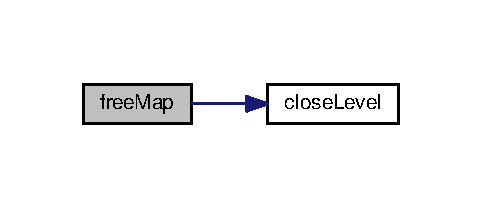
\includegraphics[width=232pt]{map_8c_ac8d4dd6fc80c79d9cb5899684740d074_cgraph}
\end{center}
\end{figure}


\hypertarget{map_8c_ace46be3df708e41a326676e6ad122bcc}{\index{map.\-c@{map.\-c}!init\-Map@{init\-Map}}
\index{init\-Map@{init\-Map}!map.c@{map.\-c}}
\paragraph[{init\-Map}]{\setlength{\rightskip}{0pt plus 5cm}{\bf Map} $\ast$ init\-Map (
\begin{DoxyParamCaption}
\item[{S\-D\-L\-\_\-\-Surface $\ast$}]{screen, }
\item[{char $\ast$}]{level\-\_\-name, }
\item[{{\bf list} $\ast$}]{l, }
\item[{{\bf platform\-Set} $\ast$}]{ps}
\end{DoxyParamCaption}
)}}\label{map_8c_ace46be3df708e41a326676e6ad122bcc}
initialize the map 
\begin{DoxyParams}[1]{Parameters}
\mbox{\tt in}  & {\em screen} & game screen \\
\hline
\mbox{\tt in}  & {\em level\-\_\-name} & lvl name \\
\hline
\mbox{\tt out}  & {\em l} & the enemy list that stocks the enemies \\
\hline
\mbox{\tt out}  & {\em ps} & the platform set for the mobile platforms \\
\hline
\end{DoxyParams}
\begin{DoxyReturn}{Returns}
pointer on the map 
\end{DoxyReturn}


Here is the call graph for this function\-:\nopagebreak
\begin{figure}[H]
\begin{center}
\leavevmode
\includegraphics[width=350pt]{map_8c_ace46be3df708e41a326676e6ad122bcc_cgraph}
\end{center}
\end{figure}


\hypertarget{map_8c_a6f031e5ad35ada9038d3a72a56053760}{\index{map.\-c@{map.\-c}!scrolling@{scrolling}}
\index{scrolling@{scrolling}!map.c@{map.\-c}}
\paragraph[{scrolling}]{\setlength{\rightskip}{0pt plus 5cm}void scrolling (
\begin{DoxyParamCaption}
\item[{{\bf Map} $\ast$}]{m, }
\item[{int}]{direction, }
\item[{float}]{speed}
\end{DoxyParamCaption}
)}}\label{map_8c_a6f031e5ad35ada9038d3a72a56053760}
scroll the map 
\begin{DoxyParams}[1]{Parameters}
\mbox{\tt in,out}  & {\em m} & the lvl \\
\hline
\mbox{\tt in}  & {\em direction} & scrolling direction \\
\hline
\mbox{\tt in}  & {\em speed} & scrolling speed \\
\hline
\end{DoxyParams}
\hypertarget{map_8c_afc8482e2afe6f96b7d6cb6ce3fc7081c}{\index{map.\-c@{map.\-c}!update\-Screen\-Map@{update\-Screen\-Map}}
\index{update\-Screen\-Map@{update\-Screen\-Map}!map.c@{map.\-c}}
\paragraph[{update\-Screen\-Map}]{\setlength{\rightskip}{0pt plus 5cm}void update\-Screen\-Map (
\begin{DoxyParamCaption}
\item[{S\-D\-L\-\_\-\-Surface $\ast$}]{screen, }
\item[{{\bf Map} $\ast$}]{m, }
\item[{char $\ast$}]{tileset}
\end{DoxyParamCaption}
)}}\label{map_8c_afc8482e2afe6f96b7d6cb6ce3fc7081c}
update and display the map 
\begin{DoxyParams}[1]{Parameters}
\mbox{\tt in,out}  & {\em screen} & \\
\hline
\mbox{\tt in}  & {\em m} & The map \\
\hline
\mbox{\tt in}  & {\em tileset} & the level tileset \\
\hline
\end{DoxyParams}


Here is the call graph for this function\-:\nopagebreak
\begin{figure}[H]
\begin{center}
\leavevmode
\includegraphics[width=302pt]{map_8c_afc8482e2afe6f96b7d6cb6ce3fc7081c_cgraph}
\end{center}
\end{figure}



\hypertarget{map_8h}{\subsection{map.\-h File Reference}
\label{map_8h}\index{map.\-h@{map.\-h}}
}


\hyperlink{map_8c}{map.\-c} header  


{\ttfamily \#include $<$stdlib.\-h$>$}\\*
{\ttfamily \#include $<$stdio.\-h$>$}\\*
{\ttfamily \#include $<$errno.\-h$>$}\\*
{\ttfamily \#include $<$S\-D\-L/\-S\-D\-L.\-h$>$}\\*
{\ttfamily \#include $<$S\-D\-L/\-S\-D\-L\-\_\-image.\-h$>$}\\*
{\ttfamily \#include \char`\"{}image.\-h\char`\"{}}\\*
{\ttfamily \#include \char`\"{}file\-\_\-level.\-h\char`\"{}}\\*
\subsubsection*{Functions}
\begin{DoxyCompactItemize}
\item 
void \hyperlink{map_8h_afc8482e2afe6f96b7d6cb6ce3fc7081c}{update\-Screen\-Map} (S\-D\-L\-\_\-\-Surface $\ast$screen, \hyperlink{struct_map}{Map} $\ast$m, char $\ast$tileset)
\item 
void \hyperlink{map_8h_a6f031e5ad35ada9038d3a72a56053760}{scrolling} (\hyperlink{struct_map}{Map} $\ast$m, int direction, float speed)
\item 
\hyperlink{struct_map}{Map} $\ast$ \hyperlink{map_8h_a4e2ce263b91d4c8915e26d5792e10747}{init\-Map} (S\-D\-L\-\_\-\-Surface $\ast$screen, char $\ast$level\-\_\-name, \hyperlink{structlist}{list} $\ast$l, \hyperlink{structplatform_set}{platform\-Set} $\ast$ps)
\item 
void \hyperlink{map_8h_ac8d4dd6fc80c79d9cb5899684740d074}{free\-Map} (\hyperlink{struct_map}{Map} $\ast$m)
\item 
int \hyperlink{map_8h_abf181167fafe365865bf0468959f1426}{collision\-Map} (S\-D\-L\-\_\-\-Rect r, \hyperlink{struct_map}{Map} $\ast$m, int type)
\end{DoxyCompactItemize}


\subsubsection{Detailed Description}
\hyperlink{map_8c}{map.\-c} header \begin{DoxyAuthor}{Author}
Xavier C\-O\-P\-O\-N\-E\-T 
\end{DoxyAuthor}
\begin{DoxyDate}{Date}
2014-\/03-\/18 
\end{DoxyDate}


\subsubsection{Function Documentation}
\hypertarget{map_8h_abf181167fafe365865bf0468959f1426}{\index{map.\-h@{map.\-h}!collision\-Map@{collision\-Map}}
\index{collision\-Map@{collision\-Map}!map.h@{map.\-h}}
\paragraph[{collision\-Map}]{\setlength{\rightskip}{0pt plus 5cm}int collision\-Map (
\begin{DoxyParamCaption}
\item[{S\-D\-L\-\_\-\-Rect}]{r, }
\item[{{\bf Map} $\ast$}]{m, }
\item[{int}]{type}
\end{DoxyParamCaption}
)}}\label{map_8h_abf181167fafe365865bf0468959f1426}
determine if there is a collision beteewen a sprite and a \char`\"{}wall\char`\"{} of the map 
\begin{DoxyParams}[1]{Parameters}
\mbox{\tt in}  & {\em r} & S\-D\-L\-\_\-\-Rect corresponding to the sprite \\
\hline
\mbox{\tt in}  & {\em m} & map \\
\hline
\mbox{\tt in}  & {\em type} & 0 if not a projectile \\
\hline
\end{DoxyParams}
\begin{DoxyReturn}{Returns}
1 if there is a collision, 0 if not,2 if collision with star/coin, 3 if spring 
\end{DoxyReturn}


Here is the call graph for this function\-:\nopagebreak
\begin{figure}[H]
\begin{center}
\leavevmode
\includegraphics[width=266pt]{map_8h_abf181167fafe365865bf0468959f1426_cgraph}
\end{center}
\end{figure}


\hypertarget{map_8h_ac8d4dd6fc80c79d9cb5899684740d074}{\index{map.\-h@{map.\-h}!free\-Map@{free\-Map}}
\index{free\-Map@{free\-Map}!map.h@{map.\-h}}
\paragraph[{free\-Map}]{\setlength{\rightskip}{0pt plus 5cm}void free\-Map (
\begin{DoxyParamCaption}
\item[{{\bf Map} $\ast$}]{m}
\end{DoxyParamCaption}
)}}\label{map_8h_ac8d4dd6fc80c79d9cb5899684740d074}
free memory allocated to the map 
\begin{DoxyParams}[1]{Parameters}
\mbox{\tt in,out}  & {\em m} & the map \\
\hline
\end{DoxyParams}


Here is the call graph for this function\-:\nopagebreak
\begin{figure}[H]
\begin{center}
\leavevmode
\includegraphics[width=232pt]{map_8h_ac8d4dd6fc80c79d9cb5899684740d074_cgraph}
\end{center}
\end{figure}


\hypertarget{map_8h_a4e2ce263b91d4c8915e26d5792e10747}{\index{map.\-h@{map.\-h}!init\-Map@{init\-Map}}
\index{init\-Map@{init\-Map}!map.h@{map.\-h}}
\paragraph[{init\-Map}]{\setlength{\rightskip}{0pt plus 5cm}{\bf Map}$\ast$ init\-Map (
\begin{DoxyParamCaption}
\item[{S\-D\-L\-\_\-\-Surface $\ast$}]{screen, }
\item[{char $\ast$}]{level\-\_\-name, }
\item[{{\bf list} $\ast$}]{l, }
\item[{{\bf platform\-Set} $\ast$}]{ps}
\end{DoxyParamCaption}
)}}\label{map_8h_a4e2ce263b91d4c8915e26d5792e10747}
initialize the map 
\begin{DoxyParams}[1]{Parameters}
\mbox{\tt in}  & {\em screen} & game screen \\
\hline
\mbox{\tt in}  & {\em level\-\_\-name} & lvl name \\
\hline
\mbox{\tt out}  & {\em l} & the enemy list that stocks the enemies \\
\hline
\mbox{\tt out}  & {\em ps} & the platform set for the mobile platforms \\
\hline
\end{DoxyParams}
\begin{DoxyReturn}{Returns}
pointer on the map 
\end{DoxyReturn}


Here is the call graph for this function\-:\nopagebreak
\begin{figure}[H]
\begin{center}
\leavevmode
\includegraphics[width=350pt]{map_8h_a4e2ce263b91d4c8915e26d5792e10747_cgraph}
\end{center}
\end{figure}


\hypertarget{map_8h_a6f031e5ad35ada9038d3a72a56053760}{\index{map.\-h@{map.\-h}!scrolling@{scrolling}}
\index{scrolling@{scrolling}!map.h@{map.\-h}}
\paragraph[{scrolling}]{\setlength{\rightskip}{0pt plus 5cm}void scrolling (
\begin{DoxyParamCaption}
\item[{{\bf Map} $\ast$}]{m, }
\item[{int}]{direction, }
\item[{float}]{speed}
\end{DoxyParamCaption}
)}}\label{map_8h_a6f031e5ad35ada9038d3a72a56053760}
scroll the map 
\begin{DoxyParams}[1]{Parameters}
\mbox{\tt in,out}  & {\em m} & the lvl \\
\hline
\mbox{\tt in}  & {\em direction} & scrolling direction \\
\hline
\mbox{\tt in}  & {\em speed} & scrolling speed \\
\hline
\end{DoxyParams}
\hypertarget{map_8h_afc8482e2afe6f96b7d6cb6ce3fc7081c}{\index{map.\-h@{map.\-h}!update\-Screen\-Map@{update\-Screen\-Map}}
\index{update\-Screen\-Map@{update\-Screen\-Map}!map.h@{map.\-h}}
\paragraph[{update\-Screen\-Map}]{\setlength{\rightskip}{0pt plus 5cm}void update\-Screen\-Map (
\begin{DoxyParamCaption}
\item[{S\-D\-L\-\_\-\-Surface $\ast$}]{screen, }
\item[{{\bf Map} $\ast$}]{m, }
\item[{char $\ast$}]{tileset}
\end{DoxyParamCaption}
)}}\label{map_8h_afc8482e2afe6f96b7d6cb6ce3fc7081c}
update and display the map 
\begin{DoxyParams}[1]{Parameters}
\mbox{\tt in,out}  & {\em screen} & \\
\hline
\mbox{\tt in}  & {\em m} & The map \\
\hline
\mbox{\tt in}  & {\em tileset} & the level tileset \\
\hline
\end{DoxyParams}


Here is the call graph for this function\-:\nopagebreak
\begin{figure}[H]
\begin{center}
\leavevmode
\includegraphics[width=302pt]{map_8h_afc8482e2afe6f96b7d6cb6ce3fc7081c_cgraph}
\end{center}
\end{figure}



\hypertarget{menu_8c}{\subsection{menu.\-c File Reference}
\label{menu_8c}\index{menu.\-c@{menu.\-c}}
}


Contain the main menu management.  


{\ttfamily \#include \char`\"{}menu.\-h\char`\"{}}\\*
\subsubsection*{Functions}
\begin{DoxyCompactItemize}
\item 
int \hyperlink{menu_8c_a9b210afb32784dfdf07bd2d4ef25e0bc}{menu} (S\-D\-L\-\_\-\-Surface $\ast$screen, int $\ast$choice, int $\ast$go)
\item 
int \hyperlink{menu_8c_a2e385684b2e6cc22168f98525f3693d8}{menu\-Tile\-Set} (S\-D\-L\-\_\-\-Surface $\ast$screen, char tile\-Set\-\_\-name\mbox{[}\hyperlink{const_8h_a9620725a4f8ab39e0912adede7cb347f}{M\-A\-X\-\_\-\-L\-E\-N\-G\-T\-H\-\_\-\-F\-I\-L\-E\-\_\-\-N\-A\-M\-E}\mbox{]})
\end{DoxyCompactItemize}


\subsubsection{Detailed Description}
Contain the main menu management. \begin{DoxyAuthor}{Author}
Glenn H\-E\-R\-R\-O\-U 
\end{DoxyAuthor}
\begin{DoxyDate}{Date}
2014-\/04-\/20 
\end{DoxyDate}


\subsubsection{Function Documentation}
\hypertarget{menu_8c_a9b210afb32784dfdf07bd2d4ef25e0bc}{\index{menu.\-c@{menu.\-c}!menu@{menu}}
\index{menu@{menu}!menu.c@{menu.\-c}}
\paragraph[{menu}]{\setlength{\rightskip}{0pt plus 5cm}int menu (
\begin{DoxyParamCaption}
\item[{S\-D\-L\-\_\-\-Surface $\ast$}]{screen, }
\item[{int $\ast$}]{choice, }
\item[{int $\ast$}]{go}
\end{DoxyParamCaption}
)}}\label{menu_8c_a9b210afb32784dfdf07bd2d4ef25e0bc}
Display the menu on the screen 
\begin{DoxyParams}[1]{Parameters}
\mbox{\tt out}  & {\em screen} & the screen of the game \\
\hline
\mbox{\tt out}  & {\em choice} & the option selected \\
\hline
\mbox{\tt out}  & {\em go} & the main loop validation \\
\hline
\end{DoxyParams}
\begin{DoxyReturn}{Returns}
1 if an option has been selected 
\end{DoxyReturn}


Here is the call graph for this function\-:\nopagebreak
\begin{figure}[H]
\begin{center}
\leavevmode
\includegraphics[width=266pt]{menu_8c_a9b210afb32784dfdf07bd2d4ef25e0bc_cgraph}
\end{center}
\end{figure}


\hypertarget{menu_8c_a2e385684b2e6cc22168f98525f3693d8}{\index{menu.\-c@{menu.\-c}!menu\-Tile\-Set@{menu\-Tile\-Set}}
\index{menu\-Tile\-Set@{menu\-Tile\-Set}!menu.c@{menu.\-c}}
\paragraph[{menu\-Tile\-Set}]{\setlength{\rightskip}{0pt plus 5cm}int menu\-Tile\-Set (
\begin{DoxyParamCaption}
\item[{S\-D\-L\-\_\-\-Surface $\ast$}]{screen, }
\item[{char}]{tile\-Set\-\_\-name\mbox{[}\-M\-A\-X\-\_\-\-L\-E\-N\-G\-T\-H\-\_\-\-F\-I\-L\-E\-\_\-\-N\-A\-M\-E\mbox{]}}
\end{DoxyParamCaption}
)}}\label{menu_8c_a2e385684b2e6cc22168f98525f3693d8}
Display the tileset menu on the screen 
\begin{DoxyParams}[1]{Parameters}
\mbox{\tt out}  & {\em screen} & the screen of the game \\
\hline
\mbox{\tt out}  & {\em tile\-Set\-\_\-name} & The name of the tile\-Set selected \\
\hline
\end{DoxyParams}
\begin{DoxyReturn}{Returns}
1 if a tileset has been selected 
\end{DoxyReturn}


Here is the call graph for this function\-:\nopagebreak
\begin{figure}[H]
\begin{center}
\leavevmode
\includegraphics[width=296pt]{menu_8c_a2e385684b2e6cc22168f98525f3693d8_cgraph}
\end{center}
\end{figure}



\hypertarget{menu_8h}{\section{menu.\-h File Reference}
\label{menu_8h}\index{menu.\-h@{menu.\-h}}
}


header de \hyperlink{menu_8c}{menu.\-c}  


{\ttfamily \#include $<$stdlib.\-h$>$}\\*
{\ttfamily \#include $<$stdio.\-h$>$}\\*
{\ttfamily \#include $<$errno.\-h$>$}\\*
{\ttfamily \#include $<$S\-D\-L/\-S\-D\-L.\-h$>$}\\*
{\ttfamily \#include $<$S\-D\-L/\-S\-D\-L\-\_\-image.\-h$>$}\\*
{\ttfamily \#include $<$S\-D\-L/\-S\-D\-L\-\_\-ttf.\-h$>$}\\*
{\ttfamily \#include \char`\"{}const.\-h\char`\"{}}\\*
{\ttfamily \#include \char`\"{}text.\-h\char`\"{}}\\*
{\ttfamily \#include \char`\"{}sound.\-h\char`\"{}}\\*
{\ttfamily \#include \char`\"{}share.\-h\char`\"{}}\\*
Include dependency graph for menu.\-h\-:
\nopagebreak
\begin{figure}[H]
\begin{center}
\leavevmode
\includegraphics[width=350pt]{menu_8h__incl}
\end{center}
\end{figure}
This graph shows which files directly or indirectly include this file\-:
\nopagebreak
\begin{figure}[H]
\begin{center}
\leavevmode
\includegraphics[width=128pt]{menu_8h__dep__incl}
\end{center}
\end{figure}
\subsection*{Functions}
\begin{DoxyCompactItemize}
\item 
\hypertarget{menu_8h_a4604196e3bcbd88eb0a7888effc9dc6f}{int {\bfseries menu} (S\-D\-L\-\_\-\-Surface $\ast$screen, int $\ast$continuer, \hyperlink{struct_sound}{Sound} $\ast$s)}\label{menu_8h_a4604196e3bcbd88eb0a7888effc9dc6f}

\item 
\hypertarget{menu_8h_a0943f574afa5b9e3928862fd99df0d4b}{Uint32 {\bfseries blink\-Text} (Uint32 intervalle, void $\ast$parametre)}\label{menu_8h_a0943f574afa5b9e3928862fd99df0d4b}

\end{DoxyCompactItemize}


\subsection{Detailed Description}
header de \hyperlink{menu_8c}{menu.\-c} \begin{DoxyAuthor}{Author}
Xavier C\-O\-P\-O\-N\-E\-T 
\end{DoxyAuthor}
\begin{DoxyDate}{Date}
2014-\/02-\/27 
\end{DoxyDate}

\hypertarget{menu__level_8c}{\section{menu\-\_\-level.\-c File Reference}
\label{menu__level_8c}\index{menu\-\_\-level.\-c@{menu\-\_\-level.\-c}}
}


level choose menu  


{\ttfamily \#include \char`\"{}menu\-\_\-level.\-h\char`\"{}}\\*
Include dependency graph for menu\-\_\-level.\-c\-:
\nopagebreak
\begin{figure}[H]
\begin{center}
\leavevmode
\includegraphics[width=350pt]{menu__level_8c__incl}
\end{center}
\end{figure}
\subsection*{Functions}
\begin{DoxyCompactItemize}
\item 
\hypertarget{menu__level_8c_a794ae7f9d9b9deb8594ec894ef18a2de}{int {\bfseries menu\-Level} (S\-D\-L\-\_\-\-Surface $\ast$screen, char level\-\_\-name\mbox{[}M\-A\-X\-\_\-\-S\-I\-Z\-E\-\_\-\-F\-I\-L\-E\-\_\-\-N\-A\-M\-E\mbox{]}, \hyperlink{struct_sound}{Sound} $\ast$sound\-\_\-sys, char player\-\_\-name\mbox{[}M\-A\-X\-\_\-\-S\-I\-Z\-E\-\_\-\-F\-I\-L\-E\-\_\-\-N\-A\-M\-E\mbox{]}, \hyperlink{struct_player}{Player} $\ast$player, int $\ast$go, int $\ast$nb\-\_\-lvl, \hyperlink{struct_input}{Input} $\ast$in)}\label{menu__level_8c_a794ae7f9d9b9deb8594ec894ef18a2de}

\end{DoxyCompactItemize}


\subsection{Detailed Description}
level choose menu \begin{DoxyAuthor}{Author}
Remi B\-E\-R\-T\-H\-O 
\end{DoxyAuthor}
\begin{DoxyDate}{Date}
15/03/14 
\end{DoxyDate}

\hypertarget{menu__level_8h}{\section{menu\-\_\-level.\-h File Reference}
\label{menu__level_8h}\index{menu\-\_\-level.\-h@{menu\-\_\-level.\-h}}
}


Menu gerant le choix du niveau.  


{\ttfamily \#include $<$stdio.\-h$>$}\\*
{\ttfamily \#include $<$stdlib.\-h$>$}\\*
{\ttfamily \#include $<$string.\-h$>$}\\*
{\ttfamily \#include $<$S\-D\-L/\-S\-D\-L.\-h$>$}\\*
{\ttfamily \#include $<$S\-D\-L/\-S\-D\-L\-\_\-image.\-h$>$}\\*
{\ttfamily \#include $<$S\-D\-L/\-S\-D\-L\-\_\-ttf.\-h$>$}\\*
{\ttfamily \#include \char`\"{}const.\-h\char`\"{}}\\*
{\ttfamily \#include \char`\"{}file\-\_\-level.\-h\char`\"{}}\\*
{\ttfamily \#include \char`\"{}share.\-h\char`\"{}}\\*
{\ttfamily \#include \char`\"{}text.\-h\char`\"{}}\\*
{\ttfamily \#include \char`\"{}sound.\-h\char`\"{}}\\*
Include dependency graph for menu\-\_\-level.\-h\-:
\nopagebreak
\begin{figure}[H]
\begin{center}
\leavevmode
\includegraphics[width=350pt]{menu__level_8h__incl}
\end{center}
\end{figure}
This graph shows which files directly or indirectly include this file\-:
\nopagebreak
\begin{figure}[H]
\begin{center}
\leavevmode
\includegraphics[width=154pt]{menu__level_8h__dep__incl}
\end{center}
\end{figure}
\subsection*{Functions}
\begin{DoxyCompactItemize}
\item 
\hypertarget{menu__level_8h_a2df6ef1e00c1fe9c46d267b8f0f56adf}{int {\bfseries menu\-Level} (S\-D\-L\-\_\-\-Surface $\ast$screen, char level\-\_\-name\mbox{[}T\-A\-I\-L\-L\-E\-\_\-\-M\-A\-X\-\_\-\-N\-O\-M\-\_\-\-F\-I\-C\-H\-I\-E\-R\mbox{]}, \hyperlink{struct_sound}{Sound} $\ast$s)}\label{menu__level_8h_a2df6ef1e00c1fe9c46d267b8f0f56adf}

\end{DoxyCompactItemize}


\subsection{Detailed Description}
Menu gerant le choix du niveau. \begin{DoxyAuthor}{Author}
Remi B\-E\-R\-T\-H\-O 
\end{DoxyAuthor}
\begin{DoxyDate}{Date}
15/03/14 
\end{DoxyDate}
\begin{DoxyVersion}{Version}
1.\-0 
\end{DoxyVersion}

\hypertarget{menu__option_8c}{\subsection{menu\-\_\-option.\-c File Reference}
\label{menu__option_8c}\index{menu\-\_\-option.\-c@{menu\-\_\-option.\-c}}
}


contain the option menu functions  


{\ttfamily \#include \char`\"{}menu\-\_\-option.\-h\char`\"{}}\\*
\subsubsection*{Functions}
\begin{DoxyCompactItemize}
\item 
int \hyperlink{menu__option_8c_a3529f1d52146bafa1f04dcf740ee0056}{menu\-Options} (S\-D\-L\-\_\-\-Surface $\ast$screen, int $\ast$go, S\-D\-L\-Key $\ast$kc)
\item 
void \hyperlink{menu__option_8c_aec745341a7cdd39be0329420a1dccc43}{key\-Board\-Options} (S\-D\-L\-\_\-\-Surface $\ast$screen, int $\ast$go, S\-D\-L\-Key $\ast$kc)
\item 
void \hyperlink{menu__option_8c_a09208fc21970afd80a59971051150a3b}{choose\-Key} (S\-D\-L\-\_\-\-Surface $\ast$screen, \hyperlink{struct_input}{Input} $\ast$in, char $\ast$action, S\-D\-L\-Key $\ast$kc, int nb)
\end{DoxyCompactItemize}


\subsubsection{Detailed Description}
contain the option menu functions \begin{DoxyAuthor}{Author}
Xavier C\-O\-P\-O\-N\-E\-T 
\end{DoxyAuthor}
\begin{DoxyDate}{Date}
2014-\/04-\/27 
\end{DoxyDate}


\subsubsection{Function Documentation}
\hypertarget{menu__option_8c_a09208fc21970afd80a59971051150a3b}{\index{menu\-\_\-option.\-c@{menu\-\_\-option.\-c}!choose\-Key@{choose\-Key}}
\index{choose\-Key@{choose\-Key}!menu_option.c@{menu\-\_\-option.\-c}}
\paragraph[{choose\-Key}]{\setlength{\rightskip}{0pt plus 5cm}void choose\-Key (
\begin{DoxyParamCaption}
\item[{S\-D\-L\-\_\-\-Surface $\ast$}]{screen, }
\item[{{\bf Input} $\ast$}]{in, }
\item[{char $\ast$}]{action, }
\item[{S\-D\-L\-Key $\ast$}]{kc, }
\item[{int}]{nb}
\end{DoxyParamCaption}
)}}\label{menu__option_8c_a09208fc21970afd80a59971051150a3b}
print the message asking the player to choose a key and wait until the player press a key and deals with this key 
\begin{DoxyParams}[1]{Parameters}
\mbox{\tt out}  & {\em screen} & the game screen \\
\hline
\mbox{\tt in,out}  & {\em in} & the input structure \\
\hline
\mbox{\tt in}  & {\em action} & the action which the key has to be choosen \\
\hline
\mbox{\tt out}  & {\em kc} & the keyboard configuration \\
\hline
\mbox{\tt in}  & {\em nb} & the number of the action \\
\hline
\end{DoxyParams}


Here is the call graph for this function\-:\nopagebreak
\begin{figure}[H]
\begin{center}
\leavevmode
\includegraphics[width=280pt]{menu__option_8c_a09208fc21970afd80a59971051150a3b_cgraph}
\end{center}
\end{figure}


\hypertarget{menu__option_8c_aec745341a7cdd39be0329420a1dccc43}{\index{menu\-\_\-option.\-c@{menu\-\_\-option.\-c}!key\-Board\-Options@{key\-Board\-Options}}
\index{key\-Board\-Options@{key\-Board\-Options}!menu_option.c@{menu\-\_\-option.\-c}}
\paragraph[{key\-Board\-Options}]{\setlength{\rightskip}{0pt plus 5cm}void key\-Board\-Options (
\begin{DoxyParamCaption}
\item[{S\-D\-L\-\_\-\-Surface $\ast$}]{screen, }
\item[{int $\ast$}]{go, }
\item[{S\-D\-L\-Key $\ast$}]{kc}
\end{DoxyParamCaption}
)}}\label{menu__option_8c_aec745341a7cdd39be0329420a1dccc43}
print the keyboard options and deals with the user choises 
\begin{DoxyParams}[1]{Parameters}
\mbox{\tt out}  & {\em screen} & the game screen \\
\hline
\mbox{\tt in,out}  & {\em go} & main loop validation \\
\hline
\mbox{\tt in,out}  & {\em kc} & the keyboard config \\
\hline
\end{DoxyParams}


Here is the call graph for this function\-:\nopagebreak
\begin{figure}[H]
\begin{center}
\leavevmode
\includegraphics[width=350pt]{menu__option_8c_aec745341a7cdd39be0329420a1dccc43_cgraph}
\end{center}
\end{figure}


\hypertarget{menu__option_8c_a3529f1d52146bafa1f04dcf740ee0056}{\index{menu\-\_\-option.\-c@{menu\-\_\-option.\-c}!menu\-Options@{menu\-Options}}
\index{menu\-Options@{menu\-Options}!menu_option.c@{menu\-\_\-option.\-c}}
\paragraph[{menu\-Options}]{\setlength{\rightskip}{0pt plus 5cm}int menu\-Options (
\begin{DoxyParamCaption}
\item[{S\-D\-L\-\_\-\-Surface $\ast$}]{screen, }
\item[{int $\ast$}]{go, }
\item[{S\-D\-L\-Key $\ast$}]{kc}
\end{DoxyParamCaption}
)}}\label{menu__option_8c_a3529f1d52146bafa1f04dcf740ee0056}
print the option menu on the screen 
\begin{DoxyParams}[1]{Parameters}
\mbox{\tt out}  & {\em screen} & the game screen \\
\hline
\mbox{\tt in,out}  & {\em go} & main loop validation \\
\hline
\mbox{\tt in,out}  & {\em kc} & the keyboard configuration \\
\hline
\end{DoxyParams}
\begin{DoxyReturn}{Returns}
the number of the option which is choosen, -\/1 if esc 
\end{DoxyReturn}


Here is the call graph for this function\-:\nopagebreak
\begin{figure}[H]
\begin{center}
\leavevmode
\includegraphics[width=298pt]{menu__option_8c_a3529f1d52146bafa1f04dcf740ee0056_cgraph}
\end{center}
\end{figure}



\hypertarget{menu__option_8h}{\subsection{menu\-\_\-option.\-h File Reference}
\label{menu__option_8h}\index{menu\-\_\-option.\-h@{menu\-\_\-option.\-h}}
}


\hyperlink{menu__option_8c}{menu\-\_\-option.\-c} header  


{\ttfamily \#include $<$stdlib.\-h$>$}\\*
{\ttfamily \#include $<$stdio.\-h$>$}\\*
{\ttfamily \#include $<$errno.\-h$>$}\\*
{\ttfamily \#include $<$S\-D\-L/\-S\-D\-L.\-h$>$}\\*
{\ttfamily \#include $<$S\-D\-L/\-S\-D\-L\-\_\-image.\-h$>$}\\*
{\ttfamily \#include $<$S\-D\-L/\-S\-D\-L\-\_\-ttf.\-h$>$}\\*
{\ttfamily \#include \char`\"{}const.\-h\char`\"{}}\\*
{\ttfamily \#include \char`\"{}text.\-h\char`\"{}}\\*
{\ttfamily \#include \char`\"{}share.\-h\char`\"{}}\\*
{\ttfamily \#include \char`\"{}image.\-h\char`\"{}}\\*
{\ttfamily \#include \char`\"{}input.\-h\char`\"{}}\\*
{\ttfamily \#include \char`\"{}option.\-h\char`\"{}}\\*
\subsubsection*{Functions}
\begin{DoxyCompactItemize}
\item 
int \hyperlink{menu__option_8h_a3529f1d52146bafa1f04dcf740ee0056}{menu\-Options} (S\-D\-L\-\_\-\-Surface $\ast$screen, int $\ast$go, S\-D\-L\-Key $\ast$kc)
\item 
void \hyperlink{menu__option_8h_aec745341a7cdd39be0329420a1dccc43}{key\-Board\-Options} (S\-D\-L\-\_\-\-Surface $\ast$screen, int $\ast$go, S\-D\-L\-Key $\ast$kc)
\item 
void \hyperlink{menu__option_8h_a09208fc21970afd80a59971051150a3b}{choose\-Key} (S\-D\-L\-\_\-\-Surface $\ast$screen, \hyperlink{struct_input}{Input} $\ast$in, char $\ast$action, S\-D\-L\-Key $\ast$kc, int nb)
\end{DoxyCompactItemize}


\subsubsection{Detailed Description}
\hyperlink{menu__option_8c}{menu\-\_\-option.\-c} header \begin{DoxyAuthor}{Author}
Xavier C\-O\-P\-O\-N\-E\-T 
\end{DoxyAuthor}
\begin{DoxyDate}{Date}
2014-\/04-\/27 
\end{DoxyDate}


\subsubsection{Function Documentation}
\hypertarget{menu__option_8h_a09208fc21970afd80a59971051150a3b}{\index{menu\-\_\-option.\-h@{menu\-\_\-option.\-h}!choose\-Key@{choose\-Key}}
\index{choose\-Key@{choose\-Key}!menu_option.h@{menu\-\_\-option.\-h}}
\paragraph[{choose\-Key}]{\setlength{\rightskip}{0pt plus 5cm}void choose\-Key (
\begin{DoxyParamCaption}
\item[{S\-D\-L\-\_\-\-Surface $\ast$}]{screen, }
\item[{{\bf Input} $\ast$}]{in, }
\item[{char $\ast$}]{action, }
\item[{S\-D\-L\-Key $\ast$}]{kc, }
\item[{int}]{nb}
\end{DoxyParamCaption}
)}}\label{menu__option_8h_a09208fc21970afd80a59971051150a3b}
print the message asking the player to choose a key and wait until the player press a key and deals with this key 
\begin{DoxyParams}[1]{Parameters}
\mbox{\tt out}  & {\em screen} & the game screen \\
\hline
\mbox{\tt in,out}  & {\em in} & the input structure \\
\hline
\mbox{\tt in}  & {\em action} & the action which the key has to be choosen \\
\hline
\mbox{\tt out}  & {\em kc} & the keyboard configuration \\
\hline
\mbox{\tt in}  & {\em nb} & the number of the action \\
\hline
\end{DoxyParams}


Here is the call graph for this function\-:
\nopagebreak
\begin{figure}[H]
\begin{center}
\leavevmode
\includegraphics[width=280pt]{menu__option_8h_a09208fc21970afd80a59971051150a3b_cgraph}
\end{center}
\end{figure}


\hypertarget{menu__option_8h_aec745341a7cdd39be0329420a1dccc43}{\index{menu\-\_\-option.\-h@{menu\-\_\-option.\-h}!key\-Board\-Options@{key\-Board\-Options}}
\index{key\-Board\-Options@{key\-Board\-Options}!menu_option.h@{menu\-\_\-option.\-h}}
\paragraph[{key\-Board\-Options}]{\setlength{\rightskip}{0pt plus 5cm}void key\-Board\-Options (
\begin{DoxyParamCaption}
\item[{S\-D\-L\-\_\-\-Surface $\ast$}]{screen, }
\item[{int $\ast$}]{go, }
\item[{S\-D\-L\-Key $\ast$}]{kc}
\end{DoxyParamCaption}
)}}\label{menu__option_8h_aec745341a7cdd39be0329420a1dccc43}
print the keyboard options and deals with the user choises 
\begin{DoxyParams}[1]{Parameters}
\mbox{\tt out}  & {\em screen} & the game screen \\
\hline
\mbox{\tt in,out}  & {\em go} & main loop validation \\
\hline
\mbox{\tt in,out}  & {\em kc} & the keyboard config \\
\hline
\end{DoxyParams}


Here is the call graph for this function\-:
\nopagebreak
\begin{figure}[H]
\begin{center}
\leavevmode
\includegraphics[width=350pt]{menu__option_8h_aec745341a7cdd39be0329420a1dccc43_cgraph}
\end{center}
\end{figure}


\hypertarget{menu__option_8h_a3529f1d52146bafa1f04dcf740ee0056}{\index{menu\-\_\-option.\-h@{menu\-\_\-option.\-h}!menu\-Options@{menu\-Options}}
\index{menu\-Options@{menu\-Options}!menu_option.h@{menu\-\_\-option.\-h}}
\paragraph[{menu\-Options}]{\setlength{\rightskip}{0pt plus 5cm}int menu\-Options (
\begin{DoxyParamCaption}
\item[{S\-D\-L\-\_\-\-Surface $\ast$}]{screen, }
\item[{int $\ast$}]{go, }
\item[{S\-D\-L\-Key $\ast$}]{kc}
\end{DoxyParamCaption}
)}}\label{menu__option_8h_a3529f1d52146bafa1f04dcf740ee0056}
print the option menu on the screen 
\begin{DoxyParams}[1]{Parameters}
\mbox{\tt out}  & {\em screen} & the game screen \\
\hline
\mbox{\tt in,out}  & {\em go} & main loop validation \\
\hline
\mbox{\tt in,out}  & {\em kc} & the keyboard configuration \\
\hline
\end{DoxyParams}
\begin{DoxyReturn}{Returns}
the number of the option which is choosen, -\/1 if esc 
\end{DoxyReturn}


Here is the call graph for this function\-:
\nopagebreak
\begin{figure}[H]
\begin{center}
\leavevmode
\includegraphics[width=298pt]{menu__option_8h_a3529f1d52146bafa1f04dcf740ee0056_cgraph}
\end{center}
\end{figure}



\hypertarget{mobile__platform_8c}{\subsection{mobile\-\_\-platform.\-c File Reference}
\label{mobile__platform_8c}\index{mobile\-\_\-platform.\-c@{mobile\-\_\-platform.\-c}}
}


contains the functions to deal with the mobile platforms  


{\ttfamily \#include \char`\"{}mobile\-\_\-platform.\-h\char`\"{}}\\*
\subsubsection*{Functions}
\begin{DoxyCompactItemize}
\item 
void \hyperlink{mobile__platform_8c_a09006b91697e96a244887fee7ca2359e}{init\-Platform\-Set} (\hyperlink{structplatform_set}{platform\-Set} $\ast$ps)
\item 
void \hyperlink{mobile__platform_8c_a80f6ef761da399b6c8d919464dc48d7e}{create\-Platform} (\hyperlink{structplatform_set}{platform\-Set} $\ast$ps, int x1, int y1, int x2, int y2)
\item 
void \hyperlink{mobile__platform_8c_a0fe4404fc8e5a9fe0df8e1cc18b91c2a}{blit\-Platform} (S\-D\-L\-\_\-\-Surface $\ast$screen, \hyperlink{structplatform_set}{platform\-Set} $\ast$ps, \hyperlink{struct_map}{Map} $\ast$m)
\item 
void \hyperlink{mobile__platform_8c_ac7f7be766f936d9c7d3cb08eaa9bddb7}{move\-Platform} (\hyperlink{struct_character}{Character} $\ast$c, \hyperlink{structplatform_set}{platform\-Set} $\ast$ps, \hyperlink{structlist}{list} $\ast$l, \hyperlink{struct_map}{Map} $\ast$m)
\item 
void \hyperlink{mobile__platform_8c_a6ac70abaaa74c1b175932c48efc38aaf}{move\-One\-Platform} (\hyperlink{struct_character}{Character} $\ast$c, \hyperlink{structplatform}{platform} $\ast$p, \hyperlink{structlist}{list} $\ast$l, int nb, \hyperlink{struct_map}{Map} $\ast$m)
\item 
int \hyperlink{mobile__platform_8c_a9bf410713b80221b6c138ba58a6fcb37}{collision\-Platform} (\hyperlink{struct_character}{Character} $\ast$c, \hyperlink{structplatform_set}{platform\-Set} $\ast$ps, S\-D\-L\-\_\-\-Rect future\-Location)
\item 
void \hyperlink{mobile__platform_8c_abe296b52d937fe5ebce22fb3682101bc}{free\-Platform\-Set} (\hyperlink{structplatform_set}{platform\-Set} $\ast$ps)
\item 
void \hyperlink{mobile__platform_8c_a31e2f2a28818722c75562e1eee0f5816}{platform\-Map} (\hyperlink{structplatform_set}{platform\-Set} $\ast$ps, S\-D\-L\-\_\-\-Rect array\mbox{[}$\,$\mbox{]}, S\-D\-L\-\_\-\-Rect mark, int vert)
\end{DoxyCompactItemize}


\subsubsection{Detailed Description}
contains the functions to deal with the mobile platforms \begin{DoxyAuthor}{Author}
X.\-C\-O\-P\-O\-N\-E\-T 
\end{DoxyAuthor}
\begin{DoxyDate}{Date}
2014-\/05-\/01 
\end{DoxyDate}


\subsubsection{Function Documentation}
\hypertarget{mobile__platform_8c_a0fe4404fc8e5a9fe0df8e1cc18b91c2a}{\index{mobile\-\_\-platform.\-c@{mobile\-\_\-platform.\-c}!blit\-Platform@{blit\-Platform}}
\index{blit\-Platform@{blit\-Platform}!mobile_platform.c@{mobile\-\_\-platform.\-c}}
\paragraph[{blit\-Platform}]{\setlength{\rightskip}{0pt plus 5cm}void blit\-Platform (
\begin{DoxyParamCaption}
\item[{S\-D\-L\-\_\-\-Surface $\ast$}]{screen, }
\item[{{\bf platform\-Set} $\ast$}]{ps, }
\item[{{\bf Map} $\ast$}]{m}
\end{DoxyParamCaption}
)}}\label{mobile__platform_8c_a0fe4404fc8e5a9fe0df8e1cc18b91c2a}
blit the platforms on the game screen 
\begin{DoxyParams}[1]{Parameters}
\mbox{\tt in,out}  & {\em screen} & game screen \\
\hline
\mbox{\tt in,out}  & {\em ps} & the platform set \\
\hline
\mbox{\tt in}  & {\em m} & the current level map \\
\hline
\end{DoxyParams}
\hypertarget{mobile__platform_8c_a9bf410713b80221b6c138ba58a6fcb37}{\index{mobile\-\_\-platform.\-c@{mobile\-\_\-platform.\-c}!collision\-Platform@{collision\-Platform}}
\index{collision\-Platform@{collision\-Platform}!mobile_platform.c@{mobile\-\_\-platform.\-c}}
\paragraph[{collision\-Platform}]{\setlength{\rightskip}{0pt plus 5cm}int collision\-Platform (
\begin{DoxyParamCaption}
\item[{{\bf Character} $\ast$}]{c, }
\item[{{\bf platform\-Set} $\ast$}]{ps, }
\item[{S\-D\-L\-\_\-\-Rect}]{future\-Location}
\end{DoxyParamCaption}
)}}\label{mobile__platform_8c_a9bf410713b80221b6c138ba58a6fcb37}
determine if there is a collision beteewen the player and a mobile platform and deals with 
\begin{DoxyParams}[1]{Parameters}
\mbox{\tt in,out}  & {\em c} & the player \\
\hline
\mbox{\tt in,out}  & {\em ps} & the platform set \\
\hline
\mbox{\tt in}  & {\em future\-Location} & the try\-Movement variabla to test the future position \\
\hline
\end{DoxyParams}
\begin{DoxyReturn}{Returns}
1 if there is a collision, 0 if not 
\end{DoxyReturn}


Here is the call graph for this function\-:\nopagebreak
\begin{figure}[H]
\begin{center}
\leavevmode
\includegraphics[width=284pt]{mobile__platform_8c_a9bf410713b80221b6c138ba58a6fcb37_cgraph}
\end{center}
\end{figure}


\hypertarget{mobile__platform_8c_a80f6ef761da399b6c8d919464dc48d7e}{\index{mobile\-\_\-platform.\-c@{mobile\-\_\-platform.\-c}!create\-Platform@{create\-Platform}}
\index{create\-Platform@{create\-Platform}!mobile_platform.c@{mobile\-\_\-platform.\-c}}
\paragraph[{create\-Platform}]{\setlength{\rightskip}{0pt plus 5cm}void create\-Platform (
\begin{DoxyParamCaption}
\item[{{\bf platform\-Set} $\ast$}]{ps, }
\item[{int}]{x1, }
\item[{int}]{y1, }
\item[{int}]{x2, }
\item[{int}]{y2}
\end{DoxyParamCaption}
)}}\label{mobile__platform_8c_a80f6ef761da399b6c8d919464dc48d7e}
creates of new platform and adds it to the platform set 
\begin{DoxyParams}[1]{Parameters}
\mbox{\tt in,out}  & {\em ps} & the platform set \\
\hline
\mbox{\tt in}  & {\em x1} & the x low limit for deplacement \\
\hline
\mbox{\tt in}  & {\em x2} & the x high limit for deplacement \\
\hline
\mbox{\tt in}  & {\em y1} & the y low limit for deplacement \\
\hline
\mbox{\tt in}  & {\em y2} & the y high limit for deplacement \\
\hline
\end{DoxyParams}


Here is the call graph for this function\-:\nopagebreak
\begin{figure}[H]
\begin{center}
\leavevmode
\includegraphics[width=286pt]{mobile__platform_8c_a80f6ef761da399b6c8d919464dc48d7e_cgraph}
\end{center}
\end{figure}


\hypertarget{mobile__platform_8c_abe296b52d937fe5ebce22fb3682101bc}{\index{mobile\-\_\-platform.\-c@{mobile\-\_\-platform.\-c}!free\-Platform\-Set@{free\-Platform\-Set}}
\index{free\-Platform\-Set@{free\-Platform\-Set}!mobile_platform.c@{mobile\-\_\-platform.\-c}}
\paragraph[{free\-Platform\-Set}]{\setlength{\rightskip}{0pt plus 5cm}void free\-Platform\-Set (
\begin{DoxyParamCaption}
\item[{{\bf platform\-Set} $\ast$}]{ps}
\end{DoxyParamCaption}
)}}\label{mobile__platform_8c_abe296b52d937fe5ebce22fb3682101bc}
free all the platforms 
\begin{DoxyParams}[1]{Parameters}
\mbox{\tt in,out}  & {\em ps} & the platform set \\
\hline
\end{DoxyParams}
\hypertarget{mobile__platform_8c_a09006b91697e96a244887fee7ca2359e}{\index{mobile\-\_\-platform.\-c@{mobile\-\_\-platform.\-c}!init\-Platform\-Set@{init\-Platform\-Set}}
\index{init\-Platform\-Set@{init\-Platform\-Set}!mobile_platform.c@{mobile\-\_\-platform.\-c}}
\paragraph[{init\-Platform\-Set}]{\setlength{\rightskip}{0pt plus 5cm}void init\-Platform\-Set (
\begin{DoxyParamCaption}
\item[{{\bf platform\-Set} $\ast$}]{ps}
\end{DoxyParamCaption}
)}}\label{mobile__platform_8c_a09006b91697e96a244887fee7ca2359e}
initialize a platform set 
\begin{DoxyParams}[1]{Parameters}
\mbox{\tt in}  & {\em ps} & the platform set to be initialized \\
\hline
\end{DoxyParams}
\hypertarget{mobile__platform_8c_a6ac70abaaa74c1b175932c48efc38aaf}{\index{mobile\-\_\-platform.\-c@{mobile\-\_\-platform.\-c}!move\-One\-Platform@{move\-One\-Platform}}
\index{move\-One\-Platform@{move\-One\-Platform}!mobile_platform.c@{mobile\-\_\-platform.\-c}}
\paragraph[{move\-One\-Platform}]{\setlength{\rightskip}{0pt plus 5cm}void move\-One\-Platform (
\begin{DoxyParamCaption}
\item[{{\bf Character} $\ast$}]{c, }
\item[{{\bf platform} $\ast$}]{p, }
\item[{{\bf list} $\ast$}]{l, }
\item[{int}]{nb, }
\item[{{\bf Map} $\ast$}]{m}
\end{DoxyParamCaption}
)}}\label{mobile__platform_8c_a6ac70abaaa74c1b175932c48efc38aaf}
moves one platforms 
\begin{DoxyParams}[1]{Parameters}
\mbox{\tt in,out}  & {\em c} & the player \\
\hline
\mbox{\tt in,out}  & {\em p} & the platform \\
\hline
\mbox{\tt in,out}  & {\em l} & the enemy list \\
\hline
\mbox{\tt in}  & {\em nb} & the number of the platform which is moved \\
\hline
\mbox{\tt in}  & {\em m} & the game map \\
\hline
\end{DoxyParams}


Here is the call graph for this function\-:\nopagebreak
\begin{figure}[H]
\begin{center}
\leavevmode
\includegraphics[width=290pt]{mobile__platform_8c_a6ac70abaaa74c1b175932c48efc38aaf_cgraph}
\end{center}
\end{figure}


\hypertarget{mobile__platform_8c_ac7f7be766f936d9c7d3cb08eaa9bddb7}{\index{mobile\-\_\-platform.\-c@{mobile\-\_\-platform.\-c}!move\-Platform@{move\-Platform}}
\index{move\-Platform@{move\-Platform}!mobile_platform.c@{mobile\-\_\-platform.\-c}}
\paragraph[{move\-Platform}]{\setlength{\rightskip}{0pt plus 5cm}void move\-Platform (
\begin{DoxyParamCaption}
\item[{{\bf Character} $\ast$}]{c, }
\item[{{\bf platform\-Set} $\ast$}]{ps, }
\item[{{\bf list} $\ast$}]{l, }
\item[{{\bf Map} $\ast$}]{m}
\end{DoxyParamCaption}
)}}\label{mobile__platform_8c_ac7f7be766f936d9c7d3cb08eaa9bddb7}
moves all the platforms 
\begin{DoxyParams}[1]{Parameters}
\mbox{\tt in,out}  & {\em c} & the player \\
\hline
\mbox{\tt in,out}  & {\em ps} & the platform set \\
\hline
\mbox{\tt in,out}  & {\em l} & the enemy list \\
\hline
\mbox{\tt in}  & {\em m} & the game map \\
\hline
\end{DoxyParams}


Here is the call graph for this function\-:\nopagebreak
\begin{figure}[H]
\begin{center}
\leavevmode
\includegraphics[width=350pt]{mobile__platform_8c_ac7f7be766f936d9c7d3cb08eaa9bddb7_cgraph}
\end{center}
\end{figure}


\hypertarget{mobile__platform_8c_a31e2f2a28818722c75562e1eee0f5816}{\index{mobile\-\_\-platform.\-c@{mobile\-\_\-platform.\-c}!platform\-Map@{platform\-Map}}
\index{platform\-Map@{platform\-Map}!mobile_platform.c@{mobile\-\_\-platform.\-c}}
\paragraph[{platform\-Map}]{\setlength{\rightskip}{0pt plus 5cm}void platform\-Map (
\begin{DoxyParamCaption}
\item[{{\bf platform\-Set} $\ast$}]{ps, }
\item[{S\-D\-L\-\_\-\-Rect}]{array\mbox{[}$\,$\mbox{]}, }
\item[{S\-D\-L\-\_\-\-Rect}]{mark, }
\item[{int}]{vert}
\end{DoxyParamCaption}
)}}\label{mobile__platform_8c_a31e2f2a28818722c75562e1eee0f5816}
takes a limit mark for a vertical deplacement platform and creates a new platform if finds another limit mark which match it, stocks it if doesn't find another limit mark 
\begin{DoxyParams}[1]{Parameters}
\mbox{\tt out}  & {\em ps} & the platform set \\
\hline
\mbox{\tt in,out}  & {\em array} & the array that stocks the limit marks \\
\hline
\mbox{\tt in}  & {\em mark} & the mark which has to be dealt with \\
\hline
\mbox{\tt in}  & {\em vert} & indicates if vertical movement(1) plarform or horizontal (0) \\
\hline
\end{DoxyParams}


Here is the call graph for this function\-:\nopagebreak
\begin{figure}[H]
\begin{center}
\leavevmode
\includegraphics[width=350pt]{mobile__platform_8c_a31e2f2a28818722c75562e1eee0f5816_cgraph}
\end{center}
\end{figure}



\hypertarget{mobile__platform_8h}{\subsection{mobile\-\_\-platform.\-h File Reference}
\label{mobile__platform_8h}\index{mobile\-\_\-platform.\-h@{mobile\-\_\-platform.\-h}}
}


\hyperlink{mobile__platform_8c}{mobile\-\_\-platform.\-c} header  


{\ttfamily \#include \char`\"{}structures.\-h\char`\"{}}\\*
{\ttfamily \#include \char`\"{}image.\-h\char`\"{}}\\*
{\ttfamily \#include \char`\"{}character.\-h\char`\"{}}\\*
\subsubsection*{Functions}
\begin{DoxyCompactItemize}
\item 
void \hyperlink{mobile__platform_8h_a09006b91697e96a244887fee7ca2359e}{init\-Platform\-Set} (\hyperlink{structplatform_set}{platform\-Set} $\ast$ps)
\item 
void \hyperlink{mobile__platform_8h_a80f6ef761da399b6c8d919464dc48d7e}{create\-Platform} (\hyperlink{structplatform_set}{platform\-Set} $\ast$ps, int x1, int y1, int x2, int y2)
\item 
void \hyperlink{mobile__platform_8h_a0fe4404fc8e5a9fe0df8e1cc18b91c2a}{blit\-Platform} (S\-D\-L\-\_\-\-Surface $\ast$screen, \hyperlink{structplatform_set}{platform\-Set} $\ast$ps, \hyperlink{struct_map}{Map} $\ast$m)
\item 
void \hyperlink{mobile__platform_8h_ac7f7be766f936d9c7d3cb08eaa9bddb7}{move\-Platform} (\hyperlink{struct_character}{Character} $\ast$c, \hyperlink{structplatform_set}{platform\-Set} $\ast$ps, \hyperlink{structlist}{list} $\ast$l, \hyperlink{struct_map}{Map} $\ast$m)
\item 
void \hyperlink{mobile__platform_8h_a6ac70abaaa74c1b175932c48efc38aaf}{move\-One\-Platform} (\hyperlink{struct_character}{Character} $\ast$c, \hyperlink{structplatform}{platform} $\ast$p, \hyperlink{structlist}{list} $\ast$l, int nb, \hyperlink{struct_map}{Map} $\ast$m)
\item 
int \hyperlink{mobile__platform_8h_a9bf410713b80221b6c138ba58a6fcb37}{collision\-Platform} (\hyperlink{struct_character}{Character} $\ast$c, \hyperlink{structplatform_set}{platform\-Set} $\ast$ps, S\-D\-L\-\_\-\-Rect future\-Location)
\item 
void \hyperlink{mobile__platform_8h_abe296b52d937fe5ebce22fb3682101bc}{free\-Platform\-Set} (\hyperlink{structplatform_set}{platform\-Set} $\ast$ps)
\item 
void \hyperlink{mobile__platform_8h_a31e2f2a28818722c75562e1eee0f5816}{platform\-Map} (\hyperlink{structplatform_set}{platform\-Set} $\ast$ps, S\-D\-L\-\_\-\-Rect array\mbox{[}$\,$\mbox{]}, S\-D\-L\-\_\-\-Rect mark, int vert)
\end{DoxyCompactItemize}


\subsubsection{Detailed Description}
\hyperlink{mobile__platform_8c}{mobile\-\_\-platform.\-c} header \begin{DoxyAuthor}{Author}
X.\-C\-O\-P\-O\-N\-E\-T 
\end{DoxyAuthor}
\begin{DoxyDate}{Date}
2014-\/05-\/01 
\end{DoxyDate}


\subsubsection{Function Documentation}
\hypertarget{mobile__platform_8h_a0fe4404fc8e5a9fe0df8e1cc18b91c2a}{\index{mobile\-\_\-platform.\-h@{mobile\-\_\-platform.\-h}!blit\-Platform@{blit\-Platform}}
\index{blit\-Platform@{blit\-Platform}!mobile_platform.h@{mobile\-\_\-platform.\-h}}
\paragraph[{blit\-Platform}]{\setlength{\rightskip}{0pt plus 5cm}void blit\-Platform (
\begin{DoxyParamCaption}
\item[{S\-D\-L\-\_\-\-Surface $\ast$}]{screen, }
\item[{{\bf platform\-Set} $\ast$}]{ps, }
\item[{{\bf Map} $\ast$}]{m}
\end{DoxyParamCaption}
)}}\label{mobile__platform_8h_a0fe4404fc8e5a9fe0df8e1cc18b91c2a}
blit the platforms on the game screen 
\begin{DoxyParams}[1]{Parameters}
\mbox{\tt in,out}  & {\em screen} & game screen \\
\hline
\mbox{\tt in,out}  & {\em ps} & the platform set \\
\hline
\mbox{\tt in}  & {\em m} & the current level map \\
\hline
\end{DoxyParams}
\hypertarget{mobile__platform_8h_a9bf410713b80221b6c138ba58a6fcb37}{\index{mobile\-\_\-platform.\-h@{mobile\-\_\-platform.\-h}!collision\-Platform@{collision\-Platform}}
\index{collision\-Platform@{collision\-Platform}!mobile_platform.h@{mobile\-\_\-platform.\-h}}
\paragraph[{collision\-Platform}]{\setlength{\rightskip}{0pt plus 5cm}int collision\-Platform (
\begin{DoxyParamCaption}
\item[{{\bf Character} $\ast$}]{c, }
\item[{{\bf platform\-Set} $\ast$}]{ps, }
\item[{S\-D\-L\-\_\-\-Rect}]{future\-Location}
\end{DoxyParamCaption}
)}}\label{mobile__platform_8h_a9bf410713b80221b6c138ba58a6fcb37}
determine if there is a collision beteewen the player and a mobile platform and deals with 
\begin{DoxyParams}[1]{Parameters}
\mbox{\tt in,out}  & {\em c} & the player \\
\hline
\mbox{\tt in,out}  & {\em ps} & the platform set \\
\hline
\mbox{\tt in}  & {\em future\-Location} & the try\-Movement variabla to test the future position \\
\hline
\end{DoxyParams}
\begin{DoxyReturn}{Returns}
1 if there is a collision, 0 if not 
\end{DoxyReturn}


Here is the call graph for this function\-:\nopagebreak
\begin{figure}[H]
\begin{center}
\leavevmode
\includegraphics[width=284pt]{mobile__platform_8h_a9bf410713b80221b6c138ba58a6fcb37_cgraph}
\end{center}
\end{figure}


\hypertarget{mobile__platform_8h_a80f6ef761da399b6c8d919464dc48d7e}{\index{mobile\-\_\-platform.\-h@{mobile\-\_\-platform.\-h}!create\-Platform@{create\-Platform}}
\index{create\-Platform@{create\-Platform}!mobile_platform.h@{mobile\-\_\-platform.\-h}}
\paragraph[{create\-Platform}]{\setlength{\rightskip}{0pt plus 5cm}void create\-Platform (
\begin{DoxyParamCaption}
\item[{{\bf platform\-Set} $\ast$}]{ps, }
\item[{int}]{x1, }
\item[{int}]{y1, }
\item[{int}]{x2, }
\item[{int}]{y2}
\end{DoxyParamCaption}
)}}\label{mobile__platform_8h_a80f6ef761da399b6c8d919464dc48d7e}
creates of new platform and adds it to the platform set 
\begin{DoxyParams}[1]{Parameters}
\mbox{\tt in,out}  & {\em ps} & the platform set \\
\hline
\mbox{\tt in}  & {\em x1} & the x low limit for deplacement \\
\hline
\mbox{\tt in}  & {\em x2} & the x high limit for deplacement \\
\hline
\mbox{\tt in}  & {\em y1} & the y low limit for deplacement \\
\hline
\mbox{\tt in}  & {\em y2} & the y high limit for deplacement \\
\hline
\end{DoxyParams}


Here is the call graph for this function\-:\nopagebreak
\begin{figure}[H]
\begin{center}
\leavevmode
\includegraphics[width=286pt]{mobile__platform_8h_a80f6ef761da399b6c8d919464dc48d7e_cgraph}
\end{center}
\end{figure}


\hypertarget{mobile__platform_8h_abe296b52d937fe5ebce22fb3682101bc}{\index{mobile\-\_\-platform.\-h@{mobile\-\_\-platform.\-h}!free\-Platform\-Set@{free\-Platform\-Set}}
\index{free\-Platform\-Set@{free\-Platform\-Set}!mobile_platform.h@{mobile\-\_\-platform.\-h}}
\paragraph[{free\-Platform\-Set}]{\setlength{\rightskip}{0pt plus 5cm}void free\-Platform\-Set (
\begin{DoxyParamCaption}
\item[{{\bf platform\-Set} $\ast$}]{ps}
\end{DoxyParamCaption}
)}}\label{mobile__platform_8h_abe296b52d937fe5ebce22fb3682101bc}
free all the platforms 
\begin{DoxyParams}[1]{Parameters}
\mbox{\tt in,out}  & {\em ps} & the platform set \\
\hline
\end{DoxyParams}
\hypertarget{mobile__platform_8h_a09006b91697e96a244887fee7ca2359e}{\index{mobile\-\_\-platform.\-h@{mobile\-\_\-platform.\-h}!init\-Platform\-Set@{init\-Platform\-Set}}
\index{init\-Platform\-Set@{init\-Platform\-Set}!mobile_platform.h@{mobile\-\_\-platform.\-h}}
\paragraph[{init\-Platform\-Set}]{\setlength{\rightskip}{0pt plus 5cm}void init\-Platform\-Set (
\begin{DoxyParamCaption}
\item[{{\bf platform\-Set} $\ast$}]{ps}
\end{DoxyParamCaption}
)}}\label{mobile__platform_8h_a09006b91697e96a244887fee7ca2359e}
initialize a platform set 
\begin{DoxyParams}[1]{Parameters}
\mbox{\tt in}  & {\em ps} & the platform set to be initialized \\
\hline
\end{DoxyParams}
\hypertarget{mobile__platform_8h_a6ac70abaaa74c1b175932c48efc38aaf}{\index{mobile\-\_\-platform.\-h@{mobile\-\_\-platform.\-h}!move\-One\-Platform@{move\-One\-Platform}}
\index{move\-One\-Platform@{move\-One\-Platform}!mobile_platform.h@{mobile\-\_\-platform.\-h}}
\paragraph[{move\-One\-Platform}]{\setlength{\rightskip}{0pt plus 5cm}void move\-One\-Platform (
\begin{DoxyParamCaption}
\item[{{\bf Character} $\ast$}]{c, }
\item[{{\bf platform} $\ast$}]{p, }
\item[{{\bf list} $\ast$}]{l, }
\item[{int}]{nb, }
\item[{{\bf Map} $\ast$}]{m}
\end{DoxyParamCaption}
)}}\label{mobile__platform_8h_a6ac70abaaa74c1b175932c48efc38aaf}
moves one platforms 
\begin{DoxyParams}[1]{Parameters}
\mbox{\tt in,out}  & {\em c} & the player \\
\hline
\mbox{\tt in,out}  & {\em p} & the platform \\
\hline
\mbox{\tt in,out}  & {\em l} & the enemy list \\
\hline
\mbox{\tt in}  & {\em nb} & the number of the platform which is moved \\
\hline
\mbox{\tt in}  & {\em m} & the game map \\
\hline
\end{DoxyParams}


Here is the call graph for this function\-:\nopagebreak
\begin{figure}[H]
\begin{center}
\leavevmode
\includegraphics[width=290pt]{mobile__platform_8h_a6ac70abaaa74c1b175932c48efc38aaf_cgraph}
\end{center}
\end{figure}


\hypertarget{mobile__platform_8h_ac7f7be766f936d9c7d3cb08eaa9bddb7}{\index{mobile\-\_\-platform.\-h@{mobile\-\_\-platform.\-h}!move\-Platform@{move\-Platform}}
\index{move\-Platform@{move\-Platform}!mobile_platform.h@{mobile\-\_\-platform.\-h}}
\paragraph[{move\-Platform}]{\setlength{\rightskip}{0pt plus 5cm}void move\-Platform (
\begin{DoxyParamCaption}
\item[{{\bf Character} $\ast$}]{c, }
\item[{{\bf platform\-Set} $\ast$}]{ps, }
\item[{{\bf list} $\ast$}]{l, }
\item[{{\bf Map} $\ast$}]{m}
\end{DoxyParamCaption}
)}}\label{mobile__platform_8h_ac7f7be766f936d9c7d3cb08eaa9bddb7}
moves all the platforms 
\begin{DoxyParams}[1]{Parameters}
\mbox{\tt in,out}  & {\em c} & the player \\
\hline
\mbox{\tt in,out}  & {\em ps} & the platform set \\
\hline
\mbox{\tt in,out}  & {\em l} & the enemy list \\
\hline
\mbox{\tt in}  & {\em m} & the game map \\
\hline
\end{DoxyParams}


Here is the call graph for this function\-:\nopagebreak
\begin{figure}[H]
\begin{center}
\leavevmode
\includegraphics[width=350pt]{mobile__platform_8h_ac7f7be766f936d9c7d3cb08eaa9bddb7_cgraph}
\end{center}
\end{figure}


\hypertarget{mobile__platform_8h_a31e2f2a28818722c75562e1eee0f5816}{\index{mobile\-\_\-platform.\-h@{mobile\-\_\-platform.\-h}!platform\-Map@{platform\-Map}}
\index{platform\-Map@{platform\-Map}!mobile_platform.h@{mobile\-\_\-platform.\-h}}
\paragraph[{platform\-Map}]{\setlength{\rightskip}{0pt plus 5cm}void platform\-Map (
\begin{DoxyParamCaption}
\item[{{\bf platform\-Set} $\ast$}]{ps, }
\item[{S\-D\-L\-\_\-\-Rect}]{array\mbox{[}$\,$\mbox{]}, }
\item[{S\-D\-L\-\_\-\-Rect}]{mark, }
\item[{int}]{vert}
\end{DoxyParamCaption}
)}}\label{mobile__platform_8h_a31e2f2a28818722c75562e1eee0f5816}
takes a limit mark for a vertical deplacement platform and creates a new platform if finds another limit mark which match it, stocks it if doesn't find another limit mark 
\begin{DoxyParams}[1]{Parameters}
\mbox{\tt out}  & {\em ps} & the platform set \\
\hline
\mbox{\tt in,out}  & {\em array} & the array that stocks the limit marks \\
\hline
\mbox{\tt in}  & {\em mark} & the mark which has to be dealt with \\
\hline
\mbox{\tt in}  & {\em vert} & indicates if vertical movement(1) plarform or horizontal (0) \\
\hline
\end{DoxyParams}


Here is the call graph for this function\-:\nopagebreak
\begin{figure}[H]
\begin{center}
\leavevmode
\includegraphics[width=350pt]{mobile__platform_8h_a31e2f2a28818722c75562e1eee0f5816_cgraph}
\end{center}
\end{figure}



\hypertarget{option_8c}{\subsection{option.\-c File Reference}
\label{option_8c}\index{option.\-c@{option.\-c}}
}


contains the funtions that manipulate the options  


{\ttfamily \#include \char`\"{}option.\-h\char`\"{}}\\*
\subsubsection*{Functions}
\begin{DoxyCompactItemize}
\item 
void \hyperlink{option_8c_a82de9e33ffe49578aedcb1796c2a524c}{load\-Sound\-Options} (char conf\-File\mbox{[}$\,$\mbox{]}, \hyperlink{struct_sound}{Sound} $\ast$sound\-Sys)
\item 
void \hyperlink{option_8c_ab75794ec6a13d9a1538d9f4fa2cb60f0}{save\-Sound\-Options} (char conf\-File\mbox{[}$\,$\mbox{]}, \hyperlink{struct_sound}{Sound} $\ast$sound\-Sys)
\item 
void \hyperlink{option_8c_a7f505e8b70cf0674aac99379c7b0a3ce}{load\-Input\-Options} (char player\-\_\-name\mbox{[}$\,$\mbox{]}, S\-D\-L\-Key $\ast$kc, \hyperlink{struct_input}{Input} $\ast$in)
\item 
void \hyperlink{option_8c_a8c9263c45096babd087bb2b1eafa0859}{save\-Input\-Options} (char player\-\_\-name\mbox{[}$\,$\mbox{]}, S\-D\-L\-Key $\ast$kc, \hyperlink{struct_input}{Input} $\ast$in)
\end{DoxyCompactItemize}


\subsubsection{Detailed Description}
contains the funtions that manipulate the options \begin{DoxyAuthor}{Author}
X.\-C\-O\-P\-O\-N\-E\-T 
\end{DoxyAuthor}
\begin{DoxyDate}{Date}
2014-\/04-\/28 
\end{DoxyDate}


\subsubsection{Function Documentation}
\hypertarget{option_8c_a7f505e8b70cf0674aac99379c7b0a3ce}{\index{option.\-c@{option.\-c}!load\-Input\-Options@{load\-Input\-Options}}
\index{load\-Input\-Options@{load\-Input\-Options}!option.c@{option.\-c}}
\paragraph[{load\-Input\-Options}]{\setlength{\rightskip}{0pt plus 5cm}void load\-Input\-Options (
\begin{DoxyParamCaption}
\item[{char}]{player\-\_\-name\mbox{[}$\,$\mbox{]}, }
\item[{S\-D\-L\-Key $\ast$}]{kc, }
\item[{{\bf Input} $\ast$}]{in}
\end{DoxyParamCaption}
)}}\label{option_8c_a7f505e8b70cf0674aac99379c7b0a3ce}
load the input options from the player input config file 
\begin{DoxyParams}[1]{Parameters}
\mbox{\tt in}  & {\em player\-\_\-name} & the current player's name \\
\hline
\mbox{\tt out}  & {\em kc} & the keyboard configuration structure \\
\hline
\mbox{\tt out}  & {\em in} & the input structure \\
\hline
\end{DoxyParams}


Here is the call graph for this function\-:
\nopagebreak
\begin{figure}[H]
\begin{center}
\leavevmode
\includegraphics[width=262pt]{option_8c_a7f505e8b70cf0674aac99379c7b0a3ce_cgraph}
\end{center}
\end{figure}


\hypertarget{option_8c_a82de9e33ffe49578aedcb1796c2a524c}{\index{option.\-c@{option.\-c}!load\-Sound\-Options@{load\-Sound\-Options}}
\index{load\-Sound\-Options@{load\-Sound\-Options}!option.c@{option.\-c}}
\paragraph[{load\-Sound\-Options}]{\setlength{\rightskip}{0pt plus 5cm}void load\-Sound\-Options (
\begin{DoxyParamCaption}
\item[{char}]{conf\-File\mbox{[}$\,$\mbox{]}, }
\item[{{\bf Sound} $\ast$}]{sound\-Sys}
\end{DoxyParamCaption}
)}}\label{option_8c_a82de9e33ffe49578aedcb1796c2a524c}
load the sound options from the sound config file 
\begin{DoxyParams}[1]{Parameters}
\mbox{\tt in}  & {\em conf\-File} & the config file path \\
\hline
\mbox{\tt out}  & {\em sound\-Sys} & the sound system \\
\hline
\end{DoxyParams}


Here is the call graph for this function\-:
\nopagebreak
\begin{figure}[H]
\begin{center}
\leavevmode
\includegraphics[width=268pt]{option_8c_a82de9e33ffe49578aedcb1796c2a524c_cgraph}
\end{center}
\end{figure}


\hypertarget{option_8c_a8c9263c45096babd087bb2b1eafa0859}{\index{option.\-c@{option.\-c}!save\-Input\-Options@{save\-Input\-Options}}
\index{save\-Input\-Options@{save\-Input\-Options}!option.c@{option.\-c}}
\paragraph[{save\-Input\-Options}]{\setlength{\rightskip}{0pt plus 5cm}void save\-Input\-Options (
\begin{DoxyParamCaption}
\item[{char}]{player\-\_\-name\mbox{[}$\,$\mbox{]}, }
\item[{S\-D\-L\-Key $\ast$}]{kc, }
\item[{{\bf Input} $\ast$}]{in}
\end{DoxyParamCaption}
)}}\label{option_8c_a8c9263c45096babd087bb2b1eafa0859}
save the input options to the player input config file 
\begin{DoxyParams}[1]{Parameters}
\mbox{\tt in}  & {\em player\-\_\-name} & the current player name \\
\hline
\mbox{\tt out}  & {\em kc} & the keyboard configuration structure \\
\hline
\mbox{\tt out}  & {\em in} & the input structure \\
\hline
\end{DoxyParams}


Here is the call graph for this function\-:
\nopagebreak
\begin{figure}[H]
\begin{center}
\leavevmode
\includegraphics[width=266pt]{option_8c_a8c9263c45096babd087bb2b1eafa0859_cgraph}
\end{center}
\end{figure}


\hypertarget{option_8c_ab75794ec6a13d9a1538d9f4fa2cb60f0}{\index{option.\-c@{option.\-c}!save\-Sound\-Options@{save\-Sound\-Options}}
\index{save\-Sound\-Options@{save\-Sound\-Options}!option.c@{option.\-c}}
\paragraph[{save\-Sound\-Options}]{\setlength{\rightskip}{0pt plus 5cm}void save\-Sound\-Options (
\begin{DoxyParamCaption}
\item[{char}]{conf\-File\mbox{[}$\,$\mbox{]}, }
\item[{{\bf Sound} $\ast$}]{sound\-Sys}
\end{DoxyParamCaption}
)}}\label{option_8c_ab75794ec6a13d9a1538d9f4fa2cb60f0}
save the sound options to the config file 
\begin{DoxyParams}[1]{Parameters}
\mbox{\tt in}  & {\em conf\-File} & the config file path \\
\hline
\mbox{\tt in}  & {\em sound\-Sys} & the sound system \\
\hline
\end{DoxyParams}


Here is the call graph for this function\-:
\nopagebreak
\begin{figure}[H]
\begin{center}
\leavevmode
\includegraphics[width=272pt]{option_8c_ab75794ec6a13d9a1538d9f4fa2cb60f0_cgraph}
\end{center}
\end{figure}



\hypertarget{option_8h}{\subsection{option.\-h File Reference}
\label{option_8h}\index{option.\-h@{option.\-h}}
}


\hyperlink{option_8c}{option.\-c} header  


{\ttfamily \#include \char`\"{}file.\-h\char`\"{}}\\*
{\ttfamily \#include \char`\"{}structures.\-h\char`\"{}}\\*
{\ttfamily \#include \char`\"{}input.\-h\char`\"{}}\\*
\subsubsection*{Functions}
\begin{DoxyCompactItemize}
\item 
void \hyperlink{option_8h_ae25f1e88b32a9246a4b222b9210fefb8}{load\-Options} (char conf\-File\mbox{[}$\,$\mbox{]}, S\-D\-L\-Key $\ast$kc)
\item 
void \hyperlink{option_8h_aa47c7d9be8978d36b12c582b701c534d}{save\-Options} (char conf\-File\mbox{[}$\,$\mbox{]}, S\-D\-L\-Key $\ast$kc)
\end{DoxyCompactItemize}


\subsubsection{Detailed Description}
\hyperlink{option_8c}{option.\-c} header \begin{DoxyAuthor}{Author}
Xavier C\-O\-P\-O\-N\-E\-T 
\end{DoxyAuthor}
\begin{DoxyDate}{Date}
2014-\/04-\/28 
\end{DoxyDate}


\subsubsection{Function Documentation}
\hypertarget{option_8h_ae25f1e88b32a9246a4b222b9210fefb8}{\index{option.\-h@{option.\-h}!load\-Options@{load\-Options}}
\index{load\-Options@{load\-Options}!option.h@{option.\-h}}
\paragraph[{load\-Options}]{\setlength{\rightskip}{0pt plus 5cm}void load\-Options (
\begin{DoxyParamCaption}
\item[{char}]{conf\-File\mbox{[}$\,$\mbox{]}, }
\item[{S\-D\-L\-Key $\ast$}]{kc}
\end{DoxyParamCaption}
)}}\label{option_8h_ae25f1e88b32a9246a4b222b9210fefb8}
Load the options from the config file 
\begin{DoxyParams}[1]{Parameters}
\mbox{\tt in}  & {\em conf\-File} & the config file path \\
\hline
\mbox{\tt out}  & {\em kc} & the keyboard configuration structure \\
\hline
\end{DoxyParams}


Here is the call graph for this function\-:
\nopagebreak
\begin{figure}[H]
\begin{center}
\leavevmode
\includegraphics[width=240pt]{option_8h_ae25f1e88b32a9246a4b222b9210fefb8_cgraph}
\end{center}
\end{figure}


\hypertarget{option_8h_aa47c7d9be8978d36b12c582b701c534d}{\index{option.\-h@{option.\-h}!save\-Options@{save\-Options}}
\index{save\-Options@{save\-Options}!option.h@{option.\-h}}
\paragraph[{save\-Options}]{\setlength{\rightskip}{0pt plus 5cm}void save\-Options (
\begin{DoxyParamCaption}
\item[{char}]{conf\-File\mbox{[}$\,$\mbox{]}, }
\item[{S\-D\-L\-Key $\ast$}]{kc}
\end{DoxyParamCaption}
)}}\label{option_8h_aa47c7d9be8978d36b12c582b701c534d}
save the options to the config file 
\begin{DoxyParams}[1]{Parameters}
\mbox{\tt in}  & {\em conf\-File} & the config file path \\
\hline
\mbox{\tt in}  & {\em kc} & the keyboard configuration structure \\
\hline
\end{DoxyParams}


Here is the call graph for this function\-:
\nopagebreak
\begin{figure}[H]
\begin{center}
\leavevmode
\includegraphics[width=244pt]{option_8h_aa47c7d9be8978d36b12c582b701c534d_cgraph}
\end{center}
\end{figure}



\hypertarget{player_8c}{\subsection{player.\-c File Reference}
\label{player_8c}\index{player.\-c@{player.\-c}}
}


Management of the player system.  


{\ttfamily \#include \char`\"{}player.\-h\char`\"{}}\\*
\subsubsection*{Functions}
\begin{DoxyCompactItemize}
\item 
int \hyperlink{player_8c_a4d30b7faab667544df4847e535dfc6e3}{new\-Player} (S\-D\-L\-\_\-\-Surface $\ast$screen, char player\-\_\-name\mbox{[}\hyperlink{const_8h_a95feb1f1a8c13ebeb7da1e49b2896c24}{M\-A\-X\-\_\-\-S\-I\-Z\-E\-\_\-\-F\-I\-L\-E\-\_\-\-N\-A\-M\-E}\mbox{]}, \hyperlink{struct_sound}{Sound} $\ast$s, int $\ast$go)
\item 
void \hyperlink{player_8c_a8330f47dea4a7c01a97ecef3607c3448}{load\-Player} (char file\-Save\mbox{[}\hyperlink{const_8h_a95feb1f1a8c13ebeb7da1e49b2896c24}{M\-A\-X\-\_\-\-S\-I\-Z\-E\-\_\-\-F\-I\-L\-E\-\_\-\-N\-A\-M\-E}\mbox{]}, char player\-\_\-name\mbox{[}\hyperlink{const_8h_a95feb1f1a8c13ebeb7da1e49b2896c24}{M\-A\-X\-\_\-\-S\-I\-Z\-E\-\_\-\-F\-I\-L\-E\-\_\-\-N\-A\-M\-E}\mbox{]}, \hyperlink{struct_player}{Player} $\ast$player)
\item 
int \hyperlink{player_8c_ac02b9148199bc3334b6c7149789c946c}{save\-Player} (char file\-Save\mbox{[}\hyperlink{const_8h_a95feb1f1a8c13ebeb7da1e49b2896c24}{M\-A\-X\-\_\-\-S\-I\-Z\-E\-\_\-\-F\-I\-L\-E\-\_\-\-N\-A\-M\-E}\mbox{]}, char player\-\_\-name\mbox{[}\hyperlink{const_8h_a95feb1f1a8c13ebeb7da1e49b2896c24}{M\-A\-X\-\_\-\-S\-I\-Z\-E\-\_\-\-F\-I\-L\-E\-\_\-\-N\-A\-M\-E}\mbox{]}, \hyperlink{struct_player}{Player} $\ast$player)
\item 
void \hyperlink{player_8c_a5bb0205907acbfde9bc8a6935e9da97e}{save} (S\-D\-L\-\_\-\-Surface $\ast$screen, char file\-Save\mbox{[}\hyperlink{const_8h_a95feb1f1a8c13ebeb7da1e49b2896c24}{M\-A\-X\-\_\-\-S\-I\-Z\-E\-\_\-\-F\-I\-L\-E\-\_\-\-N\-A\-M\-E}\mbox{]}, char player\-\_\-name\mbox{[}\hyperlink{const_8h_a95feb1f1a8c13ebeb7da1e49b2896c24}{M\-A\-X\-\_\-\-S\-I\-Z\-E\-\_\-\-F\-I\-L\-E\-\_\-\-N\-A\-M\-E}\mbox{]}, \hyperlink{struct_player}{Player} $\ast$player, int $\ast$go)
\item 
void \hyperlink{player_8c_a759d67ed182fea0f5ec9d9722c188336}{delete\-Player} (S\-D\-L\-\_\-\-Surface $\ast$screen, char file\-Save\mbox{[}\hyperlink{const_8h_a95feb1f1a8c13ebeb7da1e49b2896c24}{M\-A\-X\-\_\-\-S\-I\-Z\-E\-\_\-\-F\-I\-L\-E\-\_\-\-N\-A\-M\-E}\mbox{]}, char player\-\_\-name\mbox{[}\hyperlink{const_8h_a95feb1f1a8c13ebeb7da1e49b2896c24}{M\-A\-X\-\_\-\-S\-I\-Z\-E\-\_\-\-F\-I\-L\-E\-\_\-\-N\-A\-M\-E}\mbox{]})
\end{DoxyCompactItemize}


\subsubsection{Detailed Description}
Management of the player system. \begin{DoxyAuthor}{Author}
Glenn H\-E\-R\-R\-O\-U 
\end{DoxyAuthor}
\begin{DoxyDate}{Date}
06/05/14 
\end{DoxyDate}
\begin{DoxyVersion}{Version}
1.\-0 
\end{DoxyVersion}


\subsubsection{Function Documentation}
\hypertarget{player_8c_a759d67ed182fea0f5ec9d9722c188336}{\index{player.\-c@{player.\-c}!delete\-Player@{delete\-Player}}
\index{delete\-Player@{delete\-Player}!player.c@{player.\-c}}
\paragraph[{delete\-Player}]{\setlength{\rightskip}{0pt plus 5cm}void delete\-Player (
\begin{DoxyParamCaption}
\item[{S\-D\-L\-\_\-\-Surface $\ast$}]{screen, }
\item[{char}]{file\-Save\mbox{[}\-M\-A\-X\-\_\-\-S\-I\-Z\-E\-\_\-\-F\-I\-L\-E\-\_\-\-N\-A\-M\-E\mbox{]}, }
\item[{char}]{player\-\_\-name\mbox{[}\-M\-A\-X\-\_\-\-S\-I\-Z\-E\-\_\-\-F\-I\-L\-E\-\_\-\-N\-A\-M\-E\mbox{]}}
\end{DoxyParamCaption}
)}}\label{player_8c_a759d67ed182fea0f5ec9d9722c188336}
Delete the current player in the player list. 
\begin{DoxyParams}[1]{Parameters}
\mbox{\tt in,out}  & {\em screen} & The screen of the game \\
\hline
\mbox{\tt in,out}  & {\em file\-Save} & The path to the binary file containing the progression of each player \\
\hline
\mbox{\tt in}  & {\em player\-\_\-name} & The name of the current player \\
\hline
\end{DoxyParams}


Here is the call graph for this function\-:
\nopagebreak
\begin{figure}[H]
\begin{center}
\leavevmode
\includegraphics[width=350pt]{player_8c_a759d67ed182fea0f5ec9d9722c188336_cgraph}
\end{center}
\end{figure}


\hypertarget{player_8c_a8330f47dea4a7c01a97ecef3607c3448}{\index{player.\-c@{player.\-c}!load\-Player@{load\-Player}}
\index{load\-Player@{load\-Player}!player.c@{player.\-c}}
\paragraph[{load\-Player}]{\setlength{\rightskip}{0pt plus 5cm}void load\-Player (
\begin{DoxyParamCaption}
\item[{char}]{file\-Save\mbox{[}\-M\-A\-X\-\_\-\-S\-I\-Z\-E\-\_\-\-F\-I\-L\-E\-\_\-\-N\-A\-M\-E\mbox{]}, }
\item[{char}]{player\-\_\-name\mbox{[}\-M\-A\-X\-\_\-\-S\-I\-Z\-E\-\_\-\-F\-I\-L\-E\-\_\-\-N\-A\-M\-E\mbox{]}, }
\item[{{\bf Player} $\ast$}]{player}
\end{DoxyParamCaption}
)}}\label{player_8c_a8330f47dea4a7c01a97ecef3607c3448}
Load the progression of the given player from the binary file named file\-Save 
\begin{DoxyParams}[1]{Parameters}
\mbox{\tt in}  & {\em file\-Save} & The path to the binary file containing the progression of each player \\
\hline
\mbox{\tt in}  & {\em player\-\_\-name} & The name of the current player \\
\hline
\mbox{\tt out}  & {\em player} & The player structure where the progression will be loaded \\
\hline
\end{DoxyParams}
\hypertarget{player_8c_a4d30b7faab667544df4847e535dfc6e3}{\index{player.\-c@{player.\-c}!new\-Player@{new\-Player}}
\index{new\-Player@{new\-Player}!player.c@{player.\-c}}
\paragraph[{new\-Player}]{\setlength{\rightskip}{0pt plus 5cm}int new\-Player (
\begin{DoxyParamCaption}
\item[{S\-D\-L\-\_\-\-Surface $\ast$}]{screen, }
\item[{char}]{player\-\_\-name\mbox{[}\-M\-A\-X\-\_\-\-S\-I\-Z\-E\-\_\-\-F\-I\-L\-E\-\_\-\-N\-A\-M\-E\mbox{]}, }
\item[{{\bf Sound} $\ast$}]{s, }
\item[{int $\ast$}]{go}
\end{DoxyParamCaption}
)}}\label{player_8c_a4d30b7faab667544df4847e535dfc6e3}
Display the interface to create a new player 
\begin{DoxyParams}[1]{Parameters}
\mbox{\tt in,out}  & {\em screen} & The screen of the game \\
\hline
\mbox{\tt out}  & {\em player\-\_\-name} & The name of the new player \\
\hline
\mbox{\tt out}  & {\em s} & the sound system \\
\hline
\mbox{\tt out}  & {\em go} & the main loop validation \\
\hline
\end{DoxyParams}
\begin{DoxyReturn}{Returns}
1 if a new player has been created, 0 otherwise 
\end{DoxyReturn}


Here is the call graph for this function\-:
\nopagebreak
\begin{figure}[H]
\begin{center}
\leavevmode
\includegraphics[width=350pt]{player_8c_a4d30b7faab667544df4847e535dfc6e3_cgraph}
\end{center}
\end{figure}


\hypertarget{player_8c_a5bb0205907acbfde9bc8a6935e9da97e}{\index{player.\-c@{player.\-c}!save@{save}}
\index{save@{save}!player.c@{player.\-c}}
\paragraph[{save}]{\setlength{\rightskip}{0pt plus 5cm}void save (
\begin{DoxyParamCaption}
\item[{S\-D\-L\-\_\-\-Surface $\ast$}]{screen, }
\item[{char}]{file\-Save\mbox{[}\-M\-A\-X\-\_\-\-S\-I\-Z\-E\-\_\-\-F\-I\-L\-E\-\_\-\-N\-A\-M\-E\mbox{]}, }
\item[{char}]{player\-\_\-name\mbox{[}\-M\-A\-X\-\_\-\-S\-I\-Z\-E\-\_\-\-F\-I\-L\-E\-\_\-\-N\-A\-M\-E\mbox{]}, }
\item[{{\bf Player} $\ast$}]{player, }
\item[{int $\ast$}]{go}
\end{DoxyParamCaption}
)}}\label{player_8c_a5bb0205907acbfde9bc8a6935e9da97e}
Display the interface to save the player progression 
\begin{DoxyParams}[1]{Parameters}
\mbox{\tt in,out}  & {\em screen} & The screen of the game \\
\hline
\mbox{\tt in}  & {\em file\-Save} & The path to the binary file containing the progression of each player \\
\hline
\mbox{\tt in}  & {\em player\-\_\-name} & The name of the current player \\
\hline
\mbox{\tt out}  & {\em player} & The player structure where the progression is stored \\
\hline
\mbox{\tt out}  & {\em go} & The main loop validation \\
\hline
\end{DoxyParams}


Here is the call graph for this function\-:
\nopagebreak
\begin{figure}[H]
\begin{center}
\leavevmode
\includegraphics[width=350pt]{player_8c_a5bb0205907acbfde9bc8a6935e9da97e_cgraph}
\end{center}
\end{figure}


\hypertarget{player_8c_ac02b9148199bc3334b6c7149789c946c}{\index{player.\-c@{player.\-c}!save\-Player@{save\-Player}}
\index{save\-Player@{save\-Player}!player.c@{player.\-c}}
\paragraph[{save\-Player}]{\setlength{\rightskip}{0pt plus 5cm}int save\-Player (
\begin{DoxyParamCaption}
\item[{char}]{file\-Save\mbox{[}\-M\-A\-X\-\_\-\-S\-I\-Z\-E\-\_\-\-F\-I\-L\-E\-\_\-\-N\-A\-M\-E\mbox{]}, }
\item[{char}]{player\-\_\-name\mbox{[}\-M\-A\-X\-\_\-\-S\-I\-Z\-E\-\_\-\-F\-I\-L\-E\-\_\-\-N\-A\-M\-E\mbox{]}, }
\item[{{\bf Player} $\ast$}]{player}
\end{DoxyParamCaption}
)}}\label{player_8c_ac02b9148199bc3334b6c7149789c946c}
Save the progression of the given player in the binary file named file\-Save 
\begin{DoxyParams}[1]{Parameters}
\mbox{\tt in}  & {\em file\-Save} & The path to the binary file containing the progression of each player \\
\hline
\mbox{\tt in}  & {\em player\-\_\-name} & The name of the current player \\
\hline
\mbox{\tt out}  & {\em player} & The player structure where the progression is stored \\
\hline
\end{DoxyParams}

\hypertarget{player_8h}{\subsection{player.\-h File Reference}
\label{player_8h}\index{player.\-h@{player.\-h}}
}


\hyperlink{player_8c}{player.\-c} header  


{\ttfamily \#include $<$stdio.\-h$>$}\\*
{\ttfamily \#include $<$stdlib.\-h$>$}\\*
{\ttfamily \#include $<$string.\-h$>$}\\*
{\ttfamily \#include $<$S\-D\-L/\-S\-D\-L.\-h$>$}\\*
{\ttfamily \#include $<$S\-D\-L/\-S\-D\-L\-\_\-image.\-h$>$}\\*
{\ttfamily \#include $<$S\-D\-L/\-S\-D\-L\-\_\-ttf.\-h$>$}\\*
{\ttfamily \#include \char`\"{}const.\-h\char`\"{}}\\*
{\ttfamily \#include \char`\"{}structures.\-h\char`\"{}}\\*
{\ttfamily \#include \char`\"{}file\-\_\-level.\-h\char`\"{}}\\*
{\ttfamily \#include \char`\"{}share.\-h\char`\"{}}\\*
{\ttfamily \#include \char`\"{}text.\-h\char`\"{}}\\*
{\ttfamily \#include \char`\"{}sound.\-h\char`\"{}}\\*
{\ttfamily \#include \char`\"{}image.\-h\char`\"{}}\\*
{\ttfamily \#include \char`\"{}input.\-h\char`\"{}}\\*
\subsubsection*{Functions}
\begin{DoxyCompactItemize}
\item 
int \hyperlink{player_8h_a4d30b7faab667544df4847e535dfc6e3}{new\-Player} (S\-D\-L\-\_\-\-Surface $\ast$screen, char player\-\_\-name\mbox{[}\hyperlink{const_8h_a95feb1f1a8c13ebeb7da1e49b2896c24}{M\-A\-X\-\_\-\-S\-I\-Z\-E\-\_\-\-F\-I\-L\-E\-\_\-\-N\-A\-M\-E}\mbox{]}, \hyperlink{struct_sound}{Sound} $\ast$s, int $\ast$go)
\item 
void \hyperlink{player_8h_a8330f47dea4a7c01a97ecef3607c3448}{load\-Player} (char file\-Save\mbox{[}\hyperlink{const_8h_a95feb1f1a8c13ebeb7da1e49b2896c24}{M\-A\-X\-\_\-\-S\-I\-Z\-E\-\_\-\-F\-I\-L\-E\-\_\-\-N\-A\-M\-E}\mbox{]}, char player\-\_\-name\mbox{[}\hyperlink{const_8h_a95feb1f1a8c13ebeb7da1e49b2896c24}{M\-A\-X\-\_\-\-S\-I\-Z\-E\-\_\-\-F\-I\-L\-E\-\_\-\-N\-A\-M\-E}\mbox{]}, \hyperlink{struct_player}{Player} $\ast$player)
\item 
int \hyperlink{player_8h_ac02b9148199bc3334b6c7149789c946c}{save\-Player} (char file\-Save\mbox{[}\hyperlink{const_8h_a95feb1f1a8c13ebeb7da1e49b2896c24}{M\-A\-X\-\_\-\-S\-I\-Z\-E\-\_\-\-F\-I\-L\-E\-\_\-\-N\-A\-M\-E}\mbox{]}, char player\-\_\-name\mbox{[}\hyperlink{const_8h_a95feb1f1a8c13ebeb7da1e49b2896c24}{M\-A\-X\-\_\-\-S\-I\-Z\-E\-\_\-\-F\-I\-L\-E\-\_\-\-N\-A\-M\-E}\mbox{]}, \hyperlink{struct_player}{Player} $\ast$player)
\item 
void \hyperlink{player_8h_a5bb0205907acbfde9bc8a6935e9da97e}{save} (S\-D\-L\-\_\-\-Surface $\ast$screen, char file\-Save\mbox{[}\hyperlink{const_8h_a95feb1f1a8c13ebeb7da1e49b2896c24}{M\-A\-X\-\_\-\-S\-I\-Z\-E\-\_\-\-F\-I\-L\-E\-\_\-\-N\-A\-M\-E}\mbox{]}, char player\-\_\-name\mbox{[}\hyperlink{const_8h_a95feb1f1a8c13ebeb7da1e49b2896c24}{M\-A\-X\-\_\-\-S\-I\-Z\-E\-\_\-\-F\-I\-L\-E\-\_\-\-N\-A\-M\-E}\mbox{]}, \hyperlink{struct_player}{Player} $\ast$player, int $\ast$go)
\item 
void \hyperlink{player_8h_a759d67ed182fea0f5ec9d9722c188336}{delete\-Player} (S\-D\-L\-\_\-\-Surface $\ast$screen, char file\-Save\mbox{[}\hyperlink{const_8h_a95feb1f1a8c13ebeb7da1e49b2896c24}{M\-A\-X\-\_\-\-S\-I\-Z\-E\-\_\-\-F\-I\-L\-E\-\_\-\-N\-A\-M\-E}\mbox{]}, char player\-\_\-name\mbox{[}\hyperlink{const_8h_a95feb1f1a8c13ebeb7da1e49b2896c24}{M\-A\-X\-\_\-\-S\-I\-Z\-E\-\_\-\-F\-I\-L\-E\-\_\-\-N\-A\-M\-E}\mbox{]})
\end{DoxyCompactItemize}


\subsubsection{Detailed Description}
\hyperlink{player_8c}{player.\-c} header \begin{DoxyAuthor}{Author}
Glenn H\-E\-R\-R\-O\-U 
\end{DoxyAuthor}
\begin{DoxyDate}{Date}
06/05/14 
\end{DoxyDate}
\begin{DoxyVersion}{Version}
1.\-0 
\end{DoxyVersion}


\subsubsection{Function Documentation}
\hypertarget{player_8h_a759d67ed182fea0f5ec9d9722c188336}{\index{player.\-h@{player.\-h}!delete\-Player@{delete\-Player}}
\index{delete\-Player@{delete\-Player}!player.h@{player.\-h}}
\paragraph[{delete\-Player}]{\setlength{\rightskip}{0pt plus 5cm}void delete\-Player (
\begin{DoxyParamCaption}
\item[{S\-D\-L\-\_\-\-Surface $\ast$}]{screen, }
\item[{char}]{file\-Save\mbox{[}\-M\-A\-X\-\_\-\-S\-I\-Z\-E\-\_\-\-F\-I\-L\-E\-\_\-\-N\-A\-M\-E\mbox{]}, }
\item[{char}]{player\-\_\-name\mbox{[}\-M\-A\-X\-\_\-\-S\-I\-Z\-E\-\_\-\-F\-I\-L\-E\-\_\-\-N\-A\-M\-E\mbox{]}}
\end{DoxyParamCaption}
)}}\label{player_8h_a759d67ed182fea0f5ec9d9722c188336}
Delete the current player in the player list. 
\begin{DoxyParams}[1]{Parameters}
\mbox{\tt in,out}  & {\em screen} & The screen of the game \\
\hline
\mbox{\tt in,out}  & {\em file\-Save} & The path to the binary file containing the progression of each player \\
\hline
\mbox{\tt in}  & {\em player\-\_\-name} & The name of the current player \\
\hline
\end{DoxyParams}


Here is the call graph for this function\-:
\nopagebreak
\begin{figure}[H]
\begin{center}
\leavevmode
\includegraphics[width=350pt]{player_8h_a759d67ed182fea0f5ec9d9722c188336_cgraph}
\end{center}
\end{figure}


\hypertarget{player_8h_a8330f47dea4a7c01a97ecef3607c3448}{\index{player.\-h@{player.\-h}!load\-Player@{load\-Player}}
\index{load\-Player@{load\-Player}!player.h@{player.\-h}}
\paragraph[{load\-Player}]{\setlength{\rightskip}{0pt plus 5cm}void load\-Player (
\begin{DoxyParamCaption}
\item[{char}]{file\-Save\mbox{[}\-M\-A\-X\-\_\-\-S\-I\-Z\-E\-\_\-\-F\-I\-L\-E\-\_\-\-N\-A\-M\-E\mbox{]}, }
\item[{char}]{player\-\_\-name\mbox{[}\-M\-A\-X\-\_\-\-S\-I\-Z\-E\-\_\-\-F\-I\-L\-E\-\_\-\-N\-A\-M\-E\mbox{]}, }
\item[{{\bf Player} $\ast$}]{player}
\end{DoxyParamCaption}
)}}\label{player_8h_a8330f47dea4a7c01a97ecef3607c3448}
Load the progression of the given player from the binary file named file\-Save 
\begin{DoxyParams}[1]{Parameters}
\mbox{\tt in}  & {\em file\-Save} & The path to the binary file containing the progression of each player \\
\hline
\mbox{\tt in}  & {\em player\-\_\-name} & The name of the current player \\
\hline
\mbox{\tt out}  & {\em player} & The player structure where the progression will be loaded \\
\hline
\end{DoxyParams}
\hypertarget{player_8h_a4d30b7faab667544df4847e535dfc6e3}{\index{player.\-h@{player.\-h}!new\-Player@{new\-Player}}
\index{new\-Player@{new\-Player}!player.h@{player.\-h}}
\paragraph[{new\-Player}]{\setlength{\rightskip}{0pt plus 5cm}int new\-Player (
\begin{DoxyParamCaption}
\item[{S\-D\-L\-\_\-\-Surface $\ast$}]{screen, }
\item[{char}]{player\-\_\-name\mbox{[}\-M\-A\-X\-\_\-\-S\-I\-Z\-E\-\_\-\-F\-I\-L\-E\-\_\-\-N\-A\-M\-E\mbox{]}, }
\item[{{\bf Sound} $\ast$}]{s, }
\item[{int $\ast$}]{go}
\end{DoxyParamCaption}
)}}\label{player_8h_a4d30b7faab667544df4847e535dfc6e3}
Display the interface to create a new player 
\begin{DoxyParams}[1]{Parameters}
\mbox{\tt in,out}  & {\em screen} & The screen of the game \\
\hline
\mbox{\tt out}  & {\em player\-\_\-name} & The name of the new player \\
\hline
\mbox{\tt out}  & {\em s} & the sound system \\
\hline
\mbox{\tt out}  & {\em go} & the main loop validation \\
\hline
\end{DoxyParams}
\begin{DoxyReturn}{Returns}
1 if a new player has been created, 0 otherwise 
\end{DoxyReturn}


Here is the call graph for this function\-:
\nopagebreak
\begin{figure}[H]
\begin{center}
\leavevmode
\includegraphics[width=350pt]{player_8h_a4d30b7faab667544df4847e535dfc6e3_cgraph}
\end{center}
\end{figure}


\hypertarget{player_8h_a5bb0205907acbfde9bc8a6935e9da97e}{\index{player.\-h@{player.\-h}!save@{save}}
\index{save@{save}!player.h@{player.\-h}}
\paragraph[{save}]{\setlength{\rightskip}{0pt plus 5cm}void save (
\begin{DoxyParamCaption}
\item[{S\-D\-L\-\_\-\-Surface $\ast$}]{screen, }
\item[{char}]{file\-Save\mbox{[}\-M\-A\-X\-\_\-\-S\-I\-Z\-E\-\_\-\-F\-I\-L\-E\-\_\-\-N\-A\-M\-E\mbox{]}, }
\item[{char}]{player\-\_\-name\mbox{[}\-M\-A\-X\-\_\-\-S\-I\-Z\-E\-\_\-\-F\-I\-L\-E\-\_\-\-N\-A\-M\-E\mbox{]}, }
\item[{{\bf Player} $\ast$}]{player, }
\item[{int $\ast$}]{go}
\end{DoxyParamCaption}
)}}\label{player_8h_a5bb0205907acbfde9bc8a6935e9da97e}
Display the interface to save the player progression 
\begin{DoxyParams}[1]{Parameters}
\mbox{\tt in,out}  & {\em screen} & The screen of the game \\
\hline
\mbox{\tt in}  & {\em file\-Save} & The path to the binary file containing the progression of each player \\
\hline
\mbox{\tt in}  & {\em player\-\_\-name} & The name of the current player \\
\hline
\mbox{\tt out}  & {\em player} & The player structure where the progression is stored \\
\hline
\mbox{\tt out}  & {\em go} & The main loop validation \\
\hline
\end{DoxyParams}


Here is the call graph for this function\-:
\nopagebreak
\begin{figure}[H]
\begin{center}
\leavevmode
\includegraphics[width=350pt]{player_8h_a5bb0205907acbfde9bc8a6935e9da97e_cgraph}
\end{center}
\end{figure}


\hypertarget{player_8h_ac02b9148199bc3334b6c7149789c946c}{\index{player.\-h@{player.\-h}!save\-Player@{save\-Player}}
\index{save\-Player@{save\-Player}!player.h@{player.\-h}}
\paragraph[{save\-Player}]{\setlength{\rightskip}{0pt plus 5cm}int save\-Player (
\begin{DoxyParamCaption}
\item[{char}]{file\-Save\mbox{[}\-M\-A\-X\-\_\-\-S\-I\-Z\-E\-\_\-\-F\-I\-L\-E\-\_\-\-N\-A\-M\-E\mbox{]}, }
\item[{char}]{player\-\_\-name\mbox{[}\-M\-A\-X\-\_\-\-S\-I\-Z\-E\-\_\-\-F\-I\-L\-E\-\_\-\-N\-A\-M\-E\mbox{]}, }
\item[{{\bf Player} $\ast$}]{player}
\end{DoxyParamCaption}
)}}\label{player_8h_ac02b9148199bc3334b6c7149789c946c}
Save the progression of the given player in the binary file named file\-Save 
\begin{DoxyParams}[1]{Parameters}
\mbox{\tt in}  & {\em file\-Save} & The path to the binary file containing the progression of each player \\
\hline
\mbox{\tt in}  & {\em player\-\_\-name} & The name of the current player \\
\hline
\mbox{\tt out}  & {\em player} & The player structure where the progression is stored \\
\hline
\end{DoxyParams}

\hypertarget{projectile_8c}{\subsection{projectile.\-c File Reference}
\label{projectile_8c}\index{projectile.\-c@{projectile.\-c}}
}


contains the functions to deal with the projectiles  


{\ttfamily \#include \char`\"{}projectile.\-h\char`\"{}}\\*
\subsubsection*{Functions}
\begin{DoxyCompactItemize}
\item 
void \hyperlink{projectile_8c_a20b9e3307c60eebff33270405168dfd5}{init\-Proj\-Set} (\hyperlink{structprojectile_set}{projectile\-Set} $\ast$proj\-Set)
\item 
void \hyperlink{projectile_8c_a81ffa52ab74595ba47d07efa3455a4ee}{free\-Projectile\-Set} (\hyperlink{structprojectile_set}{projectile\-Set} $\ast$ps)
\item 
void \hyperlink{projectile_8c_ad1a769841aab1287f8f32159e2a7f768}{create\-Projectile} (\hyperlink{structprojectile_set}{projectile\-Set} $\ast$proj\-Set, char $\ast$path\-Sprite, int dir, int x, int y, int from\-N\-P\-C)
\item 
void \hyperlink{projectile_8c_a7548b539c7fb4a1f58d77f66cc381b9e}{delete\-Projectile} (\hyperlink{structprojectile_set}{projectile\-Set} $\ast$ps, int nb)
\item 
void \hyperlink{projectile_8c_a17ab2a269b02b1210842dfdf5025c0c8}{blit\-Projectile} (S\-D\-L\-\_\-\-Surface $\ast$screen, \hyperlink{structprojectile_set}{projectile\-Set} $\ast$ps, \hyperlink{struct_map}{Map} $\ast$m)
\item 
void \hyperlink{projectile_8c_a5187eabbcf884457729afaa9dc1b4053}{move\-Projectiles} (\hyperlink{struct_character}{Character} $\ast$c, \hyperlink{struct_map}{Map} $\ast$m, \hyperlink{structprojectile_set}{projectile\-Set} $\ast$ps, \hyperlink{structlist}{list} $\ast$enemy\-List)
\item 
void \hyperlink{projectile_8c_a6a0c06e7d85b486fb37bca7986f6763a}{move\-One\-Projectile} (\hyperlink{struct_character}{Character} $\ast$c, \hyperlink{struct_map}{Map} $\ast$m, \hyperlink{structprojectile_set}{projectile\-Set} $\ast$ps, \hyperlink{structlist}{list} $\ast$l, int nb)
\end{DoxyCompactItemize}


\subsubsection{Detailed Description}
contains the functions to deal with the projectiles \begin{DoxyAuthor}{Author}
X.\-C\-O\-P\-O\-N\-E\-T 
\end{DoxyAuthor}
\begin{DoxyDate}{Date}
2014-\/05-\/08 
\end{DoxyDate}


\subsubsection{Function Documentation}
\hypertarget{projectile_8c_a17ab2a269b02b1210842dfdf5025c0c8}{\index{projectile.\-c@{projectile.\-c}!blit\-Projectile@{blit\-Projectile}}
\index{blit\-Projectile@{blit\-Projectile}!projectile.c@{projectile.\-c}}
\paragraph[{blit\-Projectile}]{\setlength{\rightskip}{0pt plus 5cm}void blit\-Projectile (
\begin{DoxyParamCaption}
\item[{S\-D\-L\-\_\-\-Surface $\ast$}]{screen, }
\item[{{\bf projectile\-Set} $\ast$}]{ps, }
\item[{{\bf Map} $\ast$}]{m}
\end{DoxyParamCaption}
)}}\label{projectile_8c_a17ab2a269b02b1210842dfdf5025c0c8}
blit the projectiles on the game screen 
\begin{DoxyParams}[1]{Parameters}
\mbox{\tt in,out}  & {\em screen} & game screen \\
\hline
\mbox{\tt in,out}  & {\em ps} & the projectile set \\
\hline
\mbox{\tt in}  & {\em m} & the current level map \\
\hline
\end{DoxyParams}
\hypertarget{projectile_8c_ad1a769841aab1287f8f32159e2a7f768}{\index{projectile.\-c@{projectile.\-c}!create\-Projectile@{create\-Projectile}}
\index{create\-Projectile@{create\-Projectile}!projectile.c@{projectile.\-c}}
\paragraph[{create\-Projectile}]{\setlength{\rightskip}{0pt plus 5cm}void create\-Projectile (
\begin{DoxyParamCaption}
\item[{{\bf projectile\-Set} $\ast$}]{proj\-Set, }
\item[{char $\ast$}]{path\-Sprite, }
\item[{int}]{dir, }
\item[{int}]{x, }
\item[{int}]{y, }
\item[{int}]{from\-N\-P\-C}
\end{DoxyParamCaption}
)}}\label{projectile_8c_ad1a769841aab1287f8f32159e2a7f768}
creates a projectile and adds it to the projectile set 
\begin{DoxyParams}[1]{Parameters}
\mbox{\tt in,out}  & {\em proj\-Set} & the projectile set \\
\hline
\mbox{\tt in,out}  & {\em path\-Sprite} & the path for the sprite \\
\hline
\mbox{\tt in}  & {\em dir} & the projectile's direction \\
\hline
\mbox{\tt in}  & {\em x} & the start absciss coordinate of the projectile \\
\hline
\mbox{\tt in}  & {\em y} & the start ordinate coordinate of the projectile \\
\hline
\mbox{\tt in}  & {\em from\-N\-P\-C} & indicates if from npc or not \\
\hline
\end{DoxyParams}


Here is the call graph for this function\-:\nopagebreak
\begin{figure}[H]
\begin{center}
\leavevmode
\includegraphics[width=290pt]{projectile_8c_ad1a769841aab1287f8f32159e2a7f768_cgraph}
\end{center}
\end{figure}


\hypertarget{projectile_8c_a7548b539c7fb4a1f58d77f66cc381b9e}{\index{projectile.\-c@{projectile.\-c}!delete\-Projectile@{delete\-Projectile}}
\index{delete\-Projectile@{delete\-Projectile}!projectile.c@{projectile.\-c}}
\paragraph[{delete\-Projectile}]{\setlength{\rightskip}{0pt plus 5cm}void delete\-Projectile (
\begin{DoxyParamCaption}
\item[{{\bf projectile\-Set} $\ast$}]{ps, }
\item[{int}]{nb}
\end{DoxyParamCaption}
)}}\label{projectile_8c_a7548b539c7fb4a1f58d77f66cc381b9e}
delete a projectile 
\begin{DoxyParams}[1]{Parameters}
\mbox{\tt out}  & {\em ps} & the projectile Set \\
\hline
\mbox{\tt in}  & {\em nb} & the number of the projectile which has to be deleted \\
\hline
\end{DoxyParams}
\hypertarget{projectile_8c_a81ffa52ab74595ba47d07efa3455a4ee}{\index{projectile.\-c@{projectile.\-c}!free\-Projectile\-Set@{free\-Projectile\-Set}}
\index{free\-Projectile\-Set@{free\-Projectile\-Set}!projectile.c@{projectile.\-c}}
\paragraph[{free\-Projectile\-Set}]{\setlength{\rightskip}{0pt plus 5cm}void free\-Projectile\-Set (
\begin{DoxyParamCaption}
\item[{{\bf projectile\-Set} $\ast$}]{ps}
\end{DoxyParamCaption}
)}}\label{projectile_8c_a81ffa52ab74595ba47d07efa3455a4ee}
free all the projectiles 
\begin{DoxyParams}[1]{Parameters}
\mbox{\tt in,out}  & {\em ps} & the projectile set \\
\hline
\end{DoxyParams}
\hypertarget{projectile_8c_a20b9e3307c60eebff33270405168dfd5}{\index{projectile.\-c@{projectile.\-c}!init\-Proj\-Set@{init\-Proj\-Set}}
\index{init\-Proj\-Set@{init\-Proj\-Set}!projectile.c@{projectile.\-c}}
\paragraph[{init\-Proj\-Set}]{\setlength{\rightskip}{0pt plus 5cm}void init\-Proj\-Set (
\begin{DoxyParamCaption}
\item[{{\bf projectile\-Set} $\ast$}]{proj\-Set}
\end{DoxyParamCaption}
)}}\label{projectile_8c_a20b9e3307c60eebff33270405168dfd5}
initialize a projectile set 
\begin{DoxyParams}[1]{Parameters}
\mbox{\tt out}  & {\em proj\-Set} & the projectile set to be initialized \\
\hline
\end{DoxyParams}
\hypertarget{projectile_8c_a6a0c06e7d85b486fb37bca7986f6763a}{\index{projectile.\-c@{projectile.\-c}!move\-One\-Projectile@{move\-One\-Projectile}}
\index{move\-One\-Projectile@{move\-One\-Projectile}!projectile.c@{projectile.\-c}}
\paragraph[{move\-One\-Projectile}]{\setlength{\rightskip}{0pt plus 5cm}void move\-One\-Projectile (
\begin{DoxyParamCaption}
\item[{{\bf Character} $\ast$}]{c, }
\item[{{\bf Map} $\ast$}]{m, }
\item[{{\bf projectile\-Set} $\ast$}]{ps, }
\item[{{\bf list} $\ast$}]{l, }
\item[{int}]{nb}
\end{DoxyParamCaption}
)}}\label{projectile_8c_a6a0c06e7d85b486fb37bca7986f6763a}
moves one projectile 
\begin{DoxyParams}[1]{Parameters}
\mbox{\tt in,out}  & {\em c} & the player \\
\hline
\mbox{\tt in,out}  & {\em m} & the game map \\
\hline
\mbox{\tt in,out}  & {\em ps} & the \hyperlink{structprojectile_set}{projectile\-Set} \\
\hline
\mbox{\tt in,out}  & {\em l} & the enemy list \\
\hline
\mbox{\tt in}  & {\em nb} & the number of the projectile which is moved \\
\hline
\end{DoxyParams}


Here is the call graph for this function\-:\nopagebreak
\begin{figure}[H]
\begin{center}
\leavevmode
\includegraphics[width=350pt]{projectile_8c_a6a0c06e7d85b486fb37bca7986f6763a_cgraph}
\end{center}
\end{figure}


\hypertarget{projectile_8c_a5187eabbcf884457729afaa9dc1b4053}{\index{projectile.\-c@{projectile.\-c}!move\-Projectiles@{move\-Projectiles}}
\index{move\-Projectiles@{move\-Projectiles}!projectile.c@{projectile.\-c}}
\paragraph[{move\-Projectiles}]{\setlength{\rightskip}{0pt plus 5cm}void move\-Projectiles (
\begin{DoxyParamCaption}
\item[{{\bf Character} $\ast$}]{c, }
\item[{{\bf Map} $\ast$}]{m, }
\item[{{\bf projectile\-Set} $\ast$}]{ps, }
\item[{{\bf list} $\ast$}]{enemy\-List}
\end{DoxyParamCaption}
)}}\label{projectile_8c_a5187eabbcf884457729afaa9dc1b4053}
moves all the projectiles 
\begin{DoxyParams}[1]{Parameters}
\mbox{\tt in,out}  & {\em c} & the player \\
\hline
\mbox{\tt in,out}  & {\em m} & the game map \\
\hline
\mbox{\tt in,out}  & {\em ps} & the projectile set \\
\hline
\mbox{\tt in,out}  & {\em enemy\-List} & the enemy list \\
\hline
\end{DoxyParams}


Here is the call graph for this function\-:\nopagebreak
\begin{figure}[H]
\begin{center}
\leavevmode
\includegraphics[width=350pt]{projectile_8c_a5187eabbcf884457729afaa9dc1b4053_cgraph}
\end{center}
\end{figure}



\hypertarget{projectile_8h}{\subsection{projectile.\-h File Reference}
\label{projectile_8h}\index{projectile.\-h@{projectile.\-h}}
}


\hyperlink{projectile_8c}{projectile.\-c} header  


{\ttfamily \#include \char`\"{}structures.\-h\char`\"{}}\\*
{\ttfamily \#include \char`\"{}image.\-h\char`\"{}}\\*
{\ttfamily \#include \char`\"{}enemies.\-h\char`\"{}}\\*
{\ttfamily \#include $<$errno.\-h$>$}\\*
\subsubsection*{Functions}
\begin{DoxyCompactItemize}
\item 
void \hyperlink{projectile_8h_a20b9e3307c60eebff33270405168dfd5}{init\-Proj\-Set} (\hyperlink{structprojectile_set}{projectile\-Set} $\ast$proj\-Set)
\item 
void \hyperlink{projectile_8h_a81ffa52ab74595ba47d07efa3455a4ee}{free\-Projectile\-Set} (\hyperlink{structprojectile_set}{projectile\-Set} $\ast$ps)
\item 
void \hyperlink{projectile_8h_ad1a769841aab1287f8f32159e2a7f768}{create\-Projectile} (\hyperlink{structprojectile_set}{projectile\-Set} $\ast$proj\-Set, char $\ast$path\-Sprite, int dir, int x, int y, int from\-N\-P\-C)
\item 
void \hyperlink{projectile_8h_a7548b539c7fb4a1f58d77f66cc381b9e}{delete\-Projectile} (\hyperlink{structprojectile_set}{projectile\-Set} $\ast$ps, int nb)
\item 
void \hyperlink{projectile_8h_a17ab2a269b02b1210842dfdf5025c0c8}{blit\-Projectile} (S\-D\-L\-\_\-\-Surface $\ast$screen, \hyperlink{structprojectile_set}{projectile\-Set} $\ast$ps, \hyperlink{struct_map}{Map} $\ast$m)
\item 
void \hyperlink{projectile_8h_a5187eabbcf884457729afaa9dc1b4053}{move\-Projectiles} (\hyperlink{struct_character}{Character} $\ast$c, \hyperlink{struct_map}{Map} $\ast$m, \hyperlink{structprojectile_set}{projectile\-Set} $\ast$ps, \hyperlink{structlist}{list} $\ast$enemy\-List)
\item 
void \hyperlink{projectile_8h_a6a0c06e7d85b486fb37bca7986f6763a}{move\-One\-Projectile} (\hyperlink{struct_character}{Character} $\ast$c, \hyperlink{struct_map}{Map} $\ast$m, \hyperlink{structprojectile_set}{projectile\-Set} $\ast$ps, \hyperlink{structlist}{list} $\ast$l, int nb)
\end{DoxyCompactItemize}


\subsubsection{Detailed Description}
\hyperlink{projectile_8c}{projectile.\-c} header \begin{DoxyAuthor}{Author}
X.\-C\-O\-P\-O\-N\-E\-T 
\end{DoxyAuthor}
\begin{DoxyDate}{Date}
2014-\/05-\/08 
\end{DoxyDate}


\subsubsection{Function Documentation}
\hypertarget{projectile_8h_a17ab2a269b02b1210842dfdf5025c0c8}{\index{projectile.\-h@{projectile.\-h}!blit\-Projectile@{blit\-Projectile}}
\index{blit\-Projectile@{blit\-Projectile}!projectile.h@{projectile.\-h}}
\paragraph[{blit\-Projectile}]{\setlength{\rightskip}{0pt plus 5cm}void blit\-Projectile (
\begin{DoxyParamCaption}
\item[{S\-D\-L\-\_\-\-Surface $\ast$}]{screen, }
\item[{{\bf projectile\-Set} $\ast$}]{ps, }
\item[{{\bf Map} $\ast$}]{m}
\end{DoxyParamCaption}
)}}\label{projectile_8h_a17ab2a269b02b1210842dfdf5025c0c8}
blit the projectiles on the game screen 
\begin{DoxyParams}[1]{Parameters}
\mbox{\tt in,out}  & {\em screen} & game screen \\
\hline
\mbox{\tt in,out}  & {\em ps} & the projectile set \\
\hline
\mbox{\tt in}  & {\em m} & the current level map \\
\hline
\end{DoxyParams}
\hypertarget{projectile_8h_ad1a769841aab1287f8f32159e2a7f768}{\index{projectile.\-h@{projectile.\-h}!create\-Projectile@{create\-Projectile}}
\index{create\-Projectile@{create\-Projectile}!projectile.h@{projectile.\-h}}
\paragraph[{create\-Projectile}]{\setlength{\rightskip}{0pt plus 5cm}void create\-Projectile (
\begin{DoxyParamCaption}
\item[{{\bf projectile\-Set} $\ast$}]{proj\-Set, }
\item[{char $\ast$}]{path\-Sprite, }
\item[{int}]{dir, }
\item[{int}]{x, }
\item[{int}]{y, }
\item[{int}]{from\-N\-P\-C}
\end{DoxyParamCaption}
)}}\label{projectile_8h_ad1a769841aab1287f8f32159e2a7f768}
creates a projectile and adds it to the projectile set 
\begin{DoxyParams}[1]{Parameters}
\mbox{\tt in,out}  & {\em proj\-Set} & the projectile set \\
\hline
\mbox{\tt in,out}  & {\em path\-Sprite} & the path for the sprite \\
\hline
\mbox{\tt in}  & {\em dir} & the projectile's direction \\
\hline
\mbox{\tt in}  & {\em x} & the start absciss coordinate of the projectile \\
\hline
\mbox{\tt in}  & {\em y} & the start ordinate coordinate of the projectile \\
\hline
\mbox{\tt in}  & {\em from\-N\-P\-C} & indicates if from npc or not \\
\hline
\end{DoxyParams}


Here is the call graph for this function\-:
\nopagebreak
\begin{figure}[H]
\begin{center}
\leavevmode
\includegraphics[width=290pt]{projectile_8h_ad1a769841aab1287f8f32159e2a7f768_cgraph}
\end{center}
\end{figure}


\hypertarget{projectile_8h_a7548b539c7fb4a1f58d77f66cc381b9e}{\index{projectile.\-h@{projectile.\-h}!delete\-Projectile@{delete\-Projectile}}
\index{delete\-Projectile@{delete\-Projectile}!projectile.h@{projectile.\-h}}
\paragraph[{delete\-Projectile}]{\setlength{\rightskip}{0pt plus 5cm}void delete\-Projectile (
\begin{DoxyParamCaption}
\item[{{\bf projectile\-Set} $\ast$}]{ps, }
\item[{int}]{nb}
\end{DoxyParamCaption}
)}}\label{projectile_8h_a7548b539c7fb4a1f58d77f66cc381b9e}
delete a projectile 
\begin{DoxyParams}[1]{Parameters}
\mbox{\tt out}  & {\em ps} & the projectile Set \\
\hline
\mbox{\tt in}  & {\em nb} & the number of the projectile which has to be deleted \\
\hline
\end{DoxyParams}
\hypertarget{projectile_8h_a81ffa52ab74595ba47d07efa3455a4ee}{\index{projectile.\-h@{projectile.\-h}!free\-Projectile\-Set@{free\-Projectile\-Set}}
\index{free\-Projectile\-Set@{free\-Projectile\-Set}!projectile.h@{projectile.\-h}}
\paragraph[{free\-Projectile\-Set}]{\setlength{\rightskip}{0pt plus 5cm}void free\-Projectile\-Set (
\begin{DoxyParamCaption}
\item[{{\bf projectile\-Set} $\ast$}]{ps}
\end{DoxyParamCaption}
)}}\label{projectile_8h_a81ffa52ab74595ba47d07efa3455a4ee}
free all the projectiles 
\begin{DoxyParams}[1]{Parameters}
\mbox{\tt in,out}  & {\em ps} & the projectile set \\
\hline
\end{DoxyParams}
\hypertarget{projectile_8h_a20b9e3307c60eebff33270405168dfd5}{\index{projectile.\-h@{projectile.\-h}!init\-Proj\-Set@{init\-Proj\-Set}}
\index{init\-Proj\-Set@{init\-Proj\-Set}!projectile.h@{projectile.\-h}}
\paragraph[{init\-Proj\-Set}]{\setlength{\rightskip}{0pt plus 5cm}void init\-Proj\-Set (
\begin{DoxyParamCaption}
\item[{{\bf projectile\-Set} $\ast$}]{proj\-Set}
\end{DoxyParamCaption}
)}}\label{projectile_8h_a20b9e3307c60eebff33270405168dfd5}
initialize a projectile set 
\begin{DoxyParams}[1]{Parameters}
\mbox{\tt out}  & {\em proj\-Set} & the projectile set to be initialized \\
\hline
\end{DoxyParams}
\hypertarget{projectile_8h_a6a0c06e7d85b486fb37bca7986f6763a}{\index{projectile.\-h@{projectile.\-h}!move\-One\-Projectile@{move\-One\-Projectile}}
\index{move\-One\-Projectile@{move\-One\-Projectile}!projectile.h@{projectile.\-h}}
\paragraph[{move\-One\-Projectile}]{\setlength{\rightskip}{0pt plus 5cm}void move\-One\-Projectile (
\begin{DoxyParamCaption}
\item[{{\bf Character} $\ast$}]{c, }
\item[{{\bf Map} $\ast$}]{m, }
\item[{{\bf projectile\-Set} $\ast$}]{ps, }
\item[{{\bf list} $\ast$}]{l, }
\item[{int}]{nb}
\end{DoxyParamCaption}
)}}\label{projectile_8h_a6a0c06e7d85b486fb37bca7986f6763a}
moves one projectile 
\begin{DoxyParams}[1]{Parameters}
\mbox{\tt in,out}  & {\em c} & the player \\
\hline
\mbox{\tt in,out}  & {\em m} & the game map \\
\hline
\mbox{\tt in,out}  & {\em ps} & the \hyperlink{structprojectile_set}{projectile\-Set} \\
\hline
\mbox{\tt in,out}  & {\em l} & the enemy list \\
\hline
\mbox{\tt in}  & {\em nb} & the number of the projectile which is moved \\
\hline
\end{DoxyParams}


Here is the call graph for this function\-:
\nopagebreak
\begin{figure}[H]
\begin{center}
\leavevmode
\includegraphics[width=350pt]{projectile_8h_a6a0c06e7d85b486fb37bca7986f6763a_cgraph}
\end{center}
\end{figure}


\hypertarget{projectile_8h_a5187eabbcf884457729afaa9dc1b4053}{\index{projectile.\-h@{projectile.\-h}!move\-Projectiles@{move\-Projectiles}}
\index{move\-Projectiles@{move\-Projectiles}!projectile.h@{projectile.\-h}}
\paragraph[{move\-Projectiles}]{\setlength{\rightskip}{0pt plus 5cm}void move\-Projectiles (
\begin{DoxyParamCaption}
\item[{{\bf Character} $\ast$}]{c, }
\item[{{\bf Map} $\ast$}]{m, }
\item[{{\bf projectile\-Set} $\ast$}]{ps, }
\item[{{\bf list} $\ast$}]{enemy\-List}
\end{DoxyParamCaption}
)}}\label{projectile_8h_a5187eabbcf884457729afaa9dc1b4053}
moves all the projectiles 
\begin{DoxyParams}[1]{Parameters}
\mbox{\tt in,out}  & {\em c} & the player \\
\hline
\mbox{\tt in,out}  & {\em m} & the game map \\
\hline
\mbox{\tt in,out}  & {\em ps} & the projectile set \\
\hline
\mbox{\tt in,out}  & {\em enemy\-List} & the enemy list \\
\hline
\end{DoxyParams}


Here is the call graph for this function\-:
\nopagebreak
\begin{figure}[H]
\begin{center}
\leavevmode
\includegraphics[width=350pt]{projectile_8h_a5187eabbcf884457729afaa9dc1b4053_cgraph}
\end{center}
\end{figure}



\hypertarget{share_8c}{\subsection{share.\-c File Reference}
\label{share_8c}\index{share.\-c@{share.\-c}}
}


Management of F\-P\-S rate.  


{\ttfamily \#include \char`\"{}share.\-h\char`\"{}}\\*
\subsubsection*{Functions}
\begin{DoxyCompactItemize}
\item 
void \hyperlink{share_8c_a6e428694268169eee69c8f07827e72de}{wait\-F\-P\-S} (int $\ast$previous\-\_\-time, int $\ast$current\-\_\-time)
\end{DoxyCompactItemize}


\subsubsection{Detailed Description}
Management of F\-P\-S rate. \begin{DoxyAuthor}{Author}
Remi B\-E\-R\-T\-H\-O 
\end{DoxyAuthor}
\begin{DoxyDate}{Date}
15/03/14 
\end{DoxyDate}
\begin{DoxyVersion}{Version}
1.\-0 
\end{DoxyVersion}


\subsubsection{Function Documentation}
\hypertarget{share_8c_a6e428694268169eee69c8f07827e72de}{\index{share.\-c@{share.\-c}!wait\-F\-P\-S@{wait\-F\-P\-S}}
\index{wait\-F\-P\-S@{wait\-F\-P\-S}!share.c@{share.\-c}}
\paragraph[{wait\-F\-P\-S}]{\setlength{\rightskip}{0pt plus 5cm}void wait\-F\-P\-S (
\begin{DoxyParamCaption}
\item[{int $\ast$}]{previous\-\_\-time, }
\item[{int $\ast$}]{current\-\_\-time}
\end{DoxyParamCaption}
)}}\label{share_8c_a6e428694268169eee69c8f07827e72de}
Function managing the fps rate 
\begin{DoxyParams}[1]{Parameters}
\mbox{\tt in,out}  & {\em previous\-\_\-time} & The previous time \\
\hline
\mbox{\tt in,out}  & {\em current\-\_\-time} & The current time \\
\hline
\end{DoxyParams}

\hypertarget{share_8h}{\subsection{share.\-h File Reference}
\label{share_8h}\index{share.\-h@{share.\-h}}
}


\hyperlink{share_8c}{share.\-c} header  


{\ttfamily \#include \char`\"{}const.\-h\char`\"{}}\\*
{\ttfamily \#include $<$S\-D\-L/\-S\-D\-L.\-h$>$}\\*
\subsubsection*{Functions}
\begin{DoxyCompactItemize}
\item 
void \hyperlink{share_8h_a6e428694268169eee69c8f07827e72de}{wait\-F\-P\-S} (int $\ast$previous\-\_\-time, int $\ast$current\-\_\-time)
\end{DoxyCompactItemize}


\subsubsection{Detailed Description}
\hyperlink{share_8c}{share.\-c} header \begin{DoxyAuthor}{Author}
Remi B\-E\-R\-T\-H\-O 
\end{DoxyAuthor}
\begin{DoxyDate}{Date}
15/03/14 
\end{DoxyDate}
\begin{DoxyVersion}{Version}
1.\-0 
\end{DoxyVersion}


\subsubsection{Function Documentation}
\hypertarget{share_8h_a6e428694268169eee69c8f07827e72de}{\index{share.\-h@{share.\-h}!wait\-F\-P\-S@{wait\-F\-P\-S}}
\index{wait\-F\-P\-S@{wait\-F\-P\-S}!share.h@{share.\-h}}
\paragraph[{wait\-F\-P\-S}]{\setlength{\rightskip}{0pt plus 5cm}void wait\-F\-P\-S (
\begin{DoxyParamCaption}
\item[{int $\ast$}]{previous\-\_\-time, }
\item[{int $\ast$}]{current\-\_\-time}
\end{DoxyParamCaption}
)}}\label{share_8h_a6e428694268169eee69c8f07827e72de}
Function managing the fps rate 
\begin{DoxyParams}[1]{Parameters}
\mbox{\tt in,out}  & {\em previous\-\_\-time} & The previous time \\
\hline
\mbox{\tt in,out}  & {\em current\-\_\-time} & The current time \\
\hline
\end{DoxyParams}

\hypertarget{sound_8c}{\section{sound.\-c File Reference}
\label{sound_8c}\index{sound.\-c@{sound.\-c}}
}


contient les fonction pour jouer du son  


{\ttfamily \#include \char`\"{}sound.\-h\char`\"{}}\\*
Include dependency graph for sound.\-c\-:\nopagebreak
\begin{figure}[H]
\begin{center}
\leavevmode
\includegraphics[width=350pt]{sound_8c__incl}
\end{center}
\end{figure}
\subsection*{Functions}
\begin{DoxyCompactItemize}
\item 
\hyperlink{struct_sound}{Sound} $\ast$ \hyperlink{sound_8c_a3b1e12665aed7169d8efdb2cc611184e}{create\-Sound} (void)
\item 
void \hyperlink{sound_8c_a3af6fda5716d5f42846d0ccc01d5e2ca}{play\-Music} (\hyperlink{struct_sound}{Sound} $\ast$s, char $\ast$file)
\item 
void \hyperlink{sound_8c_a5378cbd0e1d0bfeaa823df1a8ea215f3}{play\-Music\-Once} (\hyperlink{struct_sound}{Sound} $\ast$s, char $\ast$file)
\item 
void \hyperlink{sound_8c_acc13f1ac1e0bac5afe39405869772a08}{free\-Sound} (\hyperlink{struct_sound}{Sound} $\ast$s)
\item 
void \hyperlink{sound_8c_ac3737f55b80ac35471d115d0304e8bc3}{stop\-Sound} (\hyperlink{struct_sound}{Sound} $\ast$s)
\item 
void \hyperlink{sound_8c_a63831c086cacea9358f5c86bebbfb288}{sound\-Volume} (\hyperlink{struct_sound}{Sound} $\ast$s, float volume)
\end{DoxyCompactItemize}


\subsection{Detailed Description}
contient les fonction pour jouer du son \begin{DoxyAuthor}{Author}
Xavier C\-O\-P\-O\-N\-E\-T 
\end{DoxyAuthor}
\begin{DoxyDate}{Date}
2014-\/02-\/27 
\end{DoxyDate}


\subsection{Function Documentation}
\hypertarget{sound_8c_a3b1e12665aed7169d8efdb2cc611184e}{\index{sound.\-c@{sound.\-c}!create\-Sound@{create\-Sound}}
\index{create\-Sound@{create\-Sound}!sound.c@{sound.\-c}}
\subsubsection[{create\-Sound}]{\setlength{\rightskip}{0pt plus 5cm}sound $\ast$ create\-Sound (
\begin{DoxyParamCaption}
\item[{void}]{}
\end{DoxyParamCaption}
)}}\label{sound_8c_a3b1e12665aed7169d8efdb2cc611184e}
créer une structure son \begin{DoxyReturn}{Returns}
la structure son 
\end{DoxyReturn}
\hypertarget{sound_8c_acc13f1ac1e0bac5afe39405869772a08}{\index{sound.\-c@{sound.\-c}!free\-Sound@{free\-Sound}}
\index{free\-Sound@{free\-Sound}!sound.c@{sound.\-c}}
\subsubsection[{free\-Sound}]{\setlength{\rightskip}{0pt plus 5cm}void free\-Sound (
\begin{DoxyParamCaption}
\item[{{\bf Sound} $\ast$}]{s}
\end{DoxyParamCaption}
)}}\label{sound_8c_acc13f1ac1e0bac5afe39405869772a08}
release the sound 
\begin{DoxyParams}[1]{Parameters}
\mbox{\tt out}  & {\em s} & the sound \\
\hline
\end{DoxyParams}
\hypertarget{sound_8c_a3af6fda5716d5f42846d0ccc01d5e2ca}{\index{sound.\-c@{sound.\-c}!play\-Music@{play\-Music}}
\index{play\-Music@{play\-Music}!sound.c@{sound.\-c}}
\subsubsection[{play\-Music}]{\setlength{\rightskip}{0pt plus 5cm}void play\-Music (
\begin{DoxyParamCaption}
\item[{{\bf Sound} $\ast$}]{s, }
\item[{char $\ast$}]{file}
\end{DoxyParamCaption}
)}}\label{sound_8c_a3af6fda5716d5f42846d0ccc01d5e2ca}
lit un fichier long (musique) 
\begin{DoxyParams}[1]{Parameters}
\mbox{\tt in,out}  & {\em s} & la structure son que l'on manipule \\
\hline
\mbox{\tt in}  & {\em file} & Le fichier son à lire \\
\hline
\end{DoxyParams}
\hypertarget{sound_8c_a5378cbd0e1d0bfeaa823df1a8ea215f3}{\index{sound.\-c@{sound.\-c}!play\-Music\-Once@{play\-Music\-Once}}
\index{play\-Music\-Once@{play\-Music\-Once}!sound.c@{sound.\-c}}
\subsubsection[{play\-Music\-Once}]{\setlength{\rightskip}{0pt plus 5cm}void play\-Music\-Once (
\begin{DoxyParamCaption}
\item[{{\bf Sound} $\ast$}]{s, }
\item[{char $\ast$}]{file}
\end{DoxyParamCaption}
)}}\label{sound_8c_a5378cbd0e1d0bfeaa823df1a8ea215f3}
lit un fichier long une fois 
\begin{DoxyParams}[1]{Parameters}
\mbox{\tt in,out}  & {\em s} & la structure son que l'on manipule \\
\hline
\mbox{\tt in}  & {\em file} & Le fichier son à lire \\
\hline
\end{DoxyParams}
\hypertarget{sound_8c_a63831c086cacea9358f5c86bebbfb288}{\index{sound.\-c@{sound.\-c}!sound\-Volume@{sound\-Volume}}
\index{sound\-Volume@{sound\-Volume}!sound.c@{sound.\-c}}
\subsubsection[{sound\-Volume}]{\setlength{\rightskip}{0pt plus 5cm}void sound\-Volume (
\begin{DoxyParamCaption}
\item[{{\bf Sound} $\ast$}]{s, }
\item[{float}]{volume}
\end{DoxyParamCaption}
)}}\label{sound_8c_a63831c086cacea9358f5c86bebbfb288}
set the sound volume 
\begin{DoxyParams}[1]{Parameters}
\mbox{\tt out}  & {\em s} & the sound \\
\hline
\mbox{\tt in}  & {\em volume} & the sound volume \-: \mbox{[}0.\-0 \-: no sound ; 1.\-0 (default) max power\mbox{]} \\
\hline
\end{DoxyParams}
\hypertarget{sound_8c_ac3737f55b80ac35471d115d0304e8bc3}{\index{sound.\-c@{sound.\-c}!stop\-Sound@{stop\-Sound}}
\index{stop\-Sound@{stop\-Sound}!sound.c@{sound.\-c}}
\subsubsection[{stop\-Sound}]{\setlength{\rightskip}{0pt plus 5cm}void stop\-Sound (
\begin{DoxyParamCaption}
\item[{{\bf Sound} $\ast$}]{s}
\end{DoxyParamCaption}
)}}\label{sound_8c_ac3737f55b80ac35471d115d0304e8bc3}
stop the sound 
\begin{DoxyParams}[1]{Parameters}
\mbox{\tt out}  & {\em the} & sound to stop \\
\hline
\end{DoxyParams}

\hypertarget{sound_8h}{\section{sound.\-h File Reference}
\label{sound_8h}\index{sound.\-h@{sound.\-h}}
}


header de \hyperlink{sound_8c}{sound.\-c}  


{\ttfamily \#include $<$F\-M\-O\-D/fmod.\-h$>$}\\*
{\ttfamily \#include $<$stdlib.\-h$>$}\\*
{\ttfamily \#include $<$stdio.\-h$>$}\\*
{\ttfamily \#include $<$errno.\-h$>$}\\*
Include dependency graph for sound.\-h\-:\nopagebreak
\begin{figure}[H]
\begin{center}
\leavevmode
\includegraphics[width=350pt]{sound_8h__incl}
\end{center}
\end{figure}
This graph shows which files directly or indirectly include this file\-:\nopagebreak
\begin{figure}[H]
\begin{center}
\leavevmode
\includegraphics[width=344pt]{sound_8h__dep__incl}
\end{center}
\end{figure}
\subsection*{Data Structures}
\begin{DoxyCompactItemize}
\item 
struct \hyperlink{struct_sound}{Sound}
\end{DoxyCompactItemize}
\subsection*{Functions}
\begin{DoxyCompactItemize}
\item 
\hyperlink{struct_sound}{Sound} $\ast$ \hyperlink{sound_8h_a32a66a56d175c0916741cdf8059091ba}{create\-Sound} (void)
\item 
void \hyperlink{sound_8h_a3af6fda5716d5f42846d0ccc01d5e2ca}{play\-Music} (\hyperlink{struct_sound}{Sound} $\ast$s, char $\ast$file)
\item 
void \hyperlink{sound_8h_a5378cbd0e1d0bfeaa823df1a8ea215f3}{play\-Music\-Once} (\hyperlink{struct_sound}{Sound} $\ast$s, char $\ast$file)
\item 
void \hyperlink{sound_8h_acc13f1ac1e0bac5afe39405869772a08}{free\-Sound} (\hyperlink{struct_sound}{Sound} $\ast$s)
\item 
void \hyperlink{sound_8h_ac3737f55b80ac35471d115d0304e8bc3}{stop\-Sound} (\hyperlink{struct_sound}{Sound} $\ast$s)
\item 
void \hyperlink{sound_8h_a63831c086cacea9358f5c86bebbfb288}{sound\-Volume} (\hyperlink{struct_sound}{Sound} $\ast$s, float volume)
\end{DoxyCompactItemize}


\subsection{Detailed Description}
header de \hyperlink{sound_8c}{sound.\-c} \begin{DoxyAuthor}{Author}
Xavier C\-O\-P\-O\-N\-E\-T 
\end{DoxyAuthor}
\begin{DoxyDate}{Date}
2014-\/02-\/27 
\end{DoxyDate}


\subsection{Function Documentation}
\hypertarget{sound_8h_a32a66a56d175c0916741cdf8059091ba}{\index{sound.\-h@{sound.\-h}!create\-Sound@{create\-Sound}}
\index{create\-Sound@{create\-Sound}!sound.h@{sound.\-h}}
\subsubsection[{create\-Sound}]{\setlength{\rightskip}{0pt plus 5cm}{\bf Sound}$\ast$ create\-Sound (
\begin{DoxyParamCaption}
\item[{void}]{}
\end{DoxyParamCaption}
)}}\label{sound_8h_a32a66a56d175c0916741cdf8059091ba}
créer une structure son \begin{DoxyReturn}{Returns}
la structure son 
\end{DoxyReturn}
\hypertarget{sound_8h_acc13f1ac1e0bac5afe39405869772a08}{\index{sound.\-h@{sound.\-h}!free\-Sound@{free\-Sound}}
\index{free\-Sound@{free\-Sound}!sound.h@{sound.\-h}}
\subsubsection[{free\-Sound}]{\setlength{\rightskip}{0pt plus 5cm}void free\-Sound (
\begin{DoxyParamCaption}
\item[{{\bf Sound} $\ast$}]{s}
\end{DoxyParamCaption}
)}}\label{sound_8h_acc13f1ac1e0bac5afe39405869772a08}
release the sound 
\begin{DoxyParams}[1]{Parameters}
\mbox{\tt out}  & {\em s} & the sound \\
\hline
\end{DoxyParams}
\hypertarget{sound_8h_a3af6fda5716d5f42846d0ccc01d5e2ca}{\index{sound.\-h@{sound.\-h}!play\-Music@{play\-Music}}
\index{play\-Music@{play\-Music}!sound.h@{sound.\-h}}
\subsubsection[{play\-Music}]{\setlength{\rightskip}{0pt plus 5cm}void play\-Music (
\begin{DoxyParamCaption}
\item[{{\bf Sound} $\ast$}]{s, }
\item[{char $\ast$}]{file}
\end{DoxyParamCaption}
)}}\label{sound_8h_a3af6fda5716d5f42846d0ccc01d5e2ca}
lit un fichier long (musique) 
\begin{DoxyParams}[1]{Parameters}
\mbox{\tt in,out}  & {\em s} & la structure son que l'on manipule \\
\hline
\mbox{\tt in}  & {\em file} & Le fichier son à lire \\
\hline
\end{DoxyParams}
\hypertarget{sound_8h_a5378cbd0e1d0bfeaa823df1a8ea215f3}{\index{sound.\-h@{sound.\-h}!play\-Music\-Once@{play\-Music\-Once}}
\index{play\-Music\-Once@{play\-Music\-Once}!sound.h@{sound.\-h}}
\subsubsection[{play\-Music\-Once}]{\setlength{\rightskip}{0pt plus 5cm}void play\-Music\-Once (
\begin{DoxyParamCaption}
\item[{{\bf Sound} $\ast$}]{s, }
\item[{char $\ast$}]{file}
\end{DoxyParamCaption}
)}}\label{sound_8h_a5378cbd0e1d0bfeaa823df1a8ea215f3}
lit un fichier long une fois 
\begin{DoxyParams}[1]{Parameters}
\mbox{\tt in,out}  & {\em s} & la structure son que l'on manipule \\
\hline
\mbox{\tt in}  & {\em file} & Le fichier son à lire \\
\hline
\end{DoxyParams}
\hypertarget{sound_8h_a63831c086cacea9358f5c86bebbfb288}{\index{sound.\-h@{sound.\-h}!sound\-Volume@{sound\-Volume}}
\index{sound\-Volume@{sound\-Volume}!sound.h@{sound.\-h}}
\subsubsection[{sound\-Volume}]{\setlength{\rightskip}{0pt plus 5cm}void sound\-Volume (
\begin{DoxyParamCaption}
\item[{{\bf Sound} $\ast$}]{s, }
\item[{float}]{volume}
\end{DoxyParamCaption}
)}}\label{sound_8h_a63831c086cacea9358f5c86bebbfb288}
set the sound volume 
\begin{DoxyParams}[1]{Parameters}
\mbox{\tt out}  & {\em s} & the sound \\
\hline
\mbox{\tt in}  & {\em volume} & the sound volume \-: \mbox{[}0.\-0 \-: no sound ; 1.\-0 (default) max power\mbox{]} \\
\hline
\end{DoxyParams}
\hypertarget{sound_8h_ac3737f55b80ac35471d115d0304e8bc3}{\index{sound.\-h@{sound.\-h}!stop\-Sound@{stop\-Sound}}
\index{stop\-Sound@{stop\-Sound}!sound.h@{sound.\-h}}
\subsubsection[{stop\-Sound}]{\setlength{\rightskip}{0pt plus 5cm}void stop\-Sound (
\begin{DoxyParamCaption}
\item[{{\bf Sound} $\ast$}]{s}
\end{DoxyParamCaption}
)}}\label{sound_8h_ac3737f55b80ac35471d115d0304e8bc3}
stop the sound 
\begin{DoxyParams}[1]{Parameters}
\mbox{\tt out}  & {\em the} & sound to stop \\
\hline
\end{DoxyParams}

\hypertarget{structures_8h}{\subsection{structures.\-h File Reference}
\label{structures_8h}\index{structures.\-h@{structures.\-h}}
}
{\ttfamily \#include $<$S\-D\-L/\-S\-D\-L.\-h$>$}\\*
{\ttfamily \#include \char`\"{}const.\-h\char`\"{}}\\*
\subsubsection*{Data Structures}
\begin{DoxyCompactItemize}
\item 
struct \hyperlink{struct_character}{Character}
\item 
struct \hyperlink{struct_player}{Player}
\item 
struct \hyperlink{structnode}{node}
\item 
struct \hyperlink{structlist}{list}
\item 
struct \hyperlink{structplatform}{platform}
\item 
struct \hyperlink{structplatform_set}{platform\-Set}
\item 
struct \hyperlink{structprojectile}{projectile}
\item 
struct \hyperlink{structprojectile_set}{projectile\-Set}
\item 
struct \hyperlink{struct_level}{Level}
\item 
struct \hyperlink{struct_map}{Map}
\end{DoxyCompactItemize}
\subsubsection*{Typedefs}
\begin{DoxyCompactItemize}
\item 
\hypertarget{structures_8h_af4aeda155dbe167f1c1cf38cb65bf324}{typedef struct \hyperlink{structnode}{node} {\bfseries node}}\label{structures_8h_af4aeda155dbe167f1c1cf38cb65bf324}

\end{DoxyCompactItemize}


\subsubsection{Detailed Description}
contain the definition of some structures \begin{DoxyAuthor}{Author}
X.\-C\-O\-P\-O\-N\-E\-T 
\end{DoxyAuthor}
\begin{DoxyDate}{Date}
2014-\/04-\/15 
\end{DoxyDate}

\hypertarget{text_8c}{\subsection{text.\-c File Reference}
\label{text_8c}\index{text.\-c@{text.\-c}}
}


Management of the display of text on the screen.  


{\ttfamily \#include \char`\"{}text.\-h\char`\"{}}\\*
\subsubsection*{Functions}
\begin{DoxyCompactItemize}
\item 
void \hyperlink{text_8c_a1bd80be1aff6fe5303bdd5aa80161da3}{print\-Text} (S\-D\-L\-\_\-\-Surface $\ast$screen, S\-D\-L\-\_\-\-Rect $\ast$pos\-Text, char $\ast$text, int r, int g, int b, char $\ast$font, int pt\-Size, int mode)
\item 
void \hyperlink{text_8c_abd63f9d237bb4bc462d33c00802cd7b9}{capture\-Text} (S\-D\-L\-\_\-\-Surface $\ast$screen, S\-D\-L\-\_\-\-Rect pos\-Text, char $\ast$text, int text\-\_\-length, int r, int g, int b, char $\ast$font, int text\-\_\-size, int $\ast$go)
\end{DoxyCompactItemize}


\subsubsection{Detailed Description}
Management of the display of text on the screen. \begin{DoxyAuthor}{Author}
Xavier C\-O\-P\-O\-N\-E\-T, Glenn H\-E\-R\-R\-O\-U 
\end{DoxyAuthor}
\begin{DoxyDate}{Date}
2014-\/04-\/27 
\end{DoxyDate}


\subsubsection{Function Documentation}
\hypertarget{text_8c_abd63f9d237bb4bc462d33c00802cd7b9}{\index{text.\-c@{text.\-c}!capture\-Text@{capture\-Text}}
\index{capture\-Text@{capture\-Text}!text.c@{text.\-c}}
\paragraph[{capture\-Text}]{\setlength{\rightskip}{0pt plus 5cm}void capture\-Text (
\begin{DoxyParamCaption}
\item[{S\-D\-L\-\_\-\-Surface $\ast$}]{screen, }
\item[{S\-D\-L\-\_\-\-Rect}]{pos\-Text, }
\item[{char $\ast$}]{text, }
\item[{int}]{text\-\_\-length, }
\item[{int}]{r, }
\item[{int}]{g, }
\item[{int}]{b, }
\item[{char $\ast$}]{font, }
\item[{int}]{text\-\_\-size, }
\item[{int $\ast$}]{go}
\end{DoxyParamCaption}
)}}\label{text_8c_abd63f9d237bb4bc462d33c00802cd7b9}
Capture the text corresponding to the keyboard inputs and display it on the screen at the given position 
\begin{DoxyParams}[1]{Parameters}
\mbox{\tt out}  & {\em screen} & The screen of the game \\
\hline
\mbox{\tt in}  & {\em pos\-Text} & The position of the text. If N\-U\-L\-L, the text is centered \\
\hline
\mbox{\tt out}  & {\em text} & The text to display \\
\hline
\mbox{\tt in}  & {\em r} & red value \\
\hline
\mbox{\tt in}  & {\em g} & green value \\
\hline
\mbox{\tt in}  & {\em b} & blue value \\
\hline
\mbox{\tt in}  & {\em text\-\_\-length} & the text length \\
\hline
\mbox{\tt in}  & {\em font} & The path to the font file \\
\hline
\mbox{\tt in}  & {\em text\-\_\-size} & The text size \\
\hline
\mbox{\tt out}  & {\em go} & The main loop validation \\
\hline
\end{DoxyParams}


Here is the call graph for this function\-:\nopagebreak
\begin{figure}[H]
\begin{center}
\leavevmode
\includegraphics[width=282pt]{text_8c_abd63f9d237bb4bc462d33c00802cd7b9_cgraph}
\end{center}
\end{figure}


\hypertarget{text_8c_a1bd80be1aff6fe5303bdd5aa80161da3}{\index{text.\-c@{text.\-c}!print\-Text@{print\-Text}}
\index{print\-Text@{print\-Text}!text.c@{text.\-c}}
\paragraph[{print\-Text}]{\setlength{\rightskip}{0pt plus 5cm}void print\-Text (
\begin{DoxyParamCaption}
\item[{S\-D\-L\-\_\-\-Surface $\ast$}]{screen, }
\item[{S\-D\-L\-\_\-\-Rect $\ast$}]{pos\-Text, }
\item[{char $\ast$}]{text, }
\item[{int}]{r, }
\item[{int}]{g, }
\item[{int}]{b, }
\item[{char $\ast$}]{font, }
\item[{int}]{pt\-Size, }
\item[{int}]{mode}
\end{DoxyParamCaption}
)}}\label{text_8c_a1bd80be1aff6fe5303bdd5aa80161da3}
Display the given text on the screen, at the given position 
\begin{DoxyParams}[1]{Parameters}
\mbox{\tt out}  & {\em screen} & The screen of the game \\
\hline
\mbox{\tt in}  & {\em pos\-Text} & The position of the text. If N\-U\-L\-L, the text is centered \\
\hline
\mbox{\tt in}  & {\em text} & The text to display \\
\hline
\mbox{\tt in}  & {\em r} & red value \\
\hline
\mbox{\tt in}  & {\em g} & green value \\
\hline
\mbox{\tt in}  & {\em b} & blue value \\
\hline
\mbox{\tt in}  & {\em font} & The path to the font file \\
\hline
\mbox{\tt in}  & {\em pt\-Size} & The text size \\
\hline
\mbox{\tt in}  & {\em mode} & The writing mode \-: 0 (Solid), 1 (Blended) \\
\hline
\end{DoxyParams}

\hypertarget{text_8h}{\subsection{text.\-h File Reference}
\label{text_8h}\index{text.\-h@{text.\-h}}
}


\hyperlink{text_8c}{text.\-c} header  


{\ttfamily \#include $<$stdlib.\-h$>$}\\*
{\ttfamily \#include $<$stdio.\-h$>$}\\*
{\ttfamily \#include $<$errno.\-h$>$}\\*
{\ttfamily \#include \char`\"{}structures.\-h\char`\"{}}\\*
{\ttfamily \#include $<$S\-D\-L/\-S\-D\-L.\-h$>$}\\*
{\ttfamily \#include $<$S\-D\-L/\-S\-D\-L\-\_\-image.\-h$>$}\\*
{\ttfamily \#include $<$S\-D\-L/\-S\-D\-L\-\_\-ttf.\-h$>$}\\*
{\ttfamily \#include \char`\"{}input.\-h\char`\"{}}\\*
\subsubsection*{Functions}
\begin{DoxyCompactItemize}
\item 
void \hyperlink{text_8h_a1bd80be1aff6fe5303bdd5aa80161da3}{print\-Text} (S\-D\-L\-\_\-\-Surface $\ast$screen, S\-D\-L\-\_\-\-Rect $\ast$pos\-Text, char $\ast$text, int r, int g, int b, char $\ast$font, int pt\-Size, int mode)
\item 
void \hyperlink{text_8h_abd63f9d237bb4bc462d33c00802cd7b9}{capture\-Text} (S\-D\-L\-\_\-\-Surface $\ast$screen, S\-D\-L\-\_\-\-Rect pos\-Text, char $\ast$text, int text\-\_\-length, int r, int g, int b, char $\ast$font, int text\-\_\-size, int $\ast$go)
\end{DoxyCompactItemize}


\subsubsection{Detailed Description}
\hyperlink{text_8c}{text.\-c} header \begin{DoxyAuthor}{Author}
Xavier C\-O\-P\-O\-N\-E\-T, Glenn H\-E\-R\-R\-O\-U 
\end{DoxyAuthor}
\begin{DoxyDate}{Date}
2014-\/04-\/27 
\end{DoxyDate}


\subsubsection{Function Documentation}
\hypertarget{text_8h_abd63f9d237bb4bc462d33c00802cd7b9}{\index{text.\-h@{text.\-h}!capture\-Text@{capture\-Text}}
\index{capture\-Text@{capture\-Text}!text.h@{text.\-h}}
\paragraph[{capture\-Text}]{\setlength{\rightskip}{0pt plus 5cm}void capture\-Text (
\begin{DoxyParamCaption}
\item[{S\-D\-L\-\_\-\-Surface $\ast$}]{screen, }
\item[{S\-D\-L\-\_\-\-Rect}]{pos\-Text, }
\item[{char $\ast$}]{text, }
\item[{int}]{text\-\_\-length, }
\item[{int}]{r, }
\item[{int}]{g, }
\item[{int}]{b, }
\item[{char $\ast$}]{font, }
\item[{int}]{text\-\_\-size, }
\item[{int $\ast$}]{go}
\end{DoxyParamCaption}
)}}\label{text_8h_abd63f9d237bb4bc462d33c00802cd7b9}
Capture the text corresponding to the keyboard inputs and display it on the screen at the given position 
\begin{DoxyParams}[1]{Parameters}
\mbox{\tt out}  & {\em screen} & The screen of the game \\
\hline
\mbox{\tt in}  & {\em pos\-Text} & The position of the text. If N\-U\-L\-L, the text is centered \\
\hline
\mbox{\tt out}  & {\em text} & The text to display \\
\hline
\mbox{\tt in}  & {\em r} & red value \\
\hline
\mbox{\tt in}  & {\em g} & green value \\
\hline
\mbox{\tt in}  & {\em b} & blue value \\
\hline
\mbox{\tt in}  & {\em text\-\_\-length} & the text length \\
\hline
\mbox{\tt in}  & {\em font} & The path to the font file \\
\hline
\mbox{\tt in}  & {\em text\-\_\-size} & The text size \\
\hline
\mbox{\tt out}  & {\em go} & The main loop validation \\
\hline
\end{DoxyParams}


Here is the call graph for this function\-:\nopagebreak
\begin{figure}[H]
\begin{center}
\leavevmode
\includegraphics[width=282pt]{text_8h_abd63f9d237bb4bc462d33c00802cd7b9_cgraph}
\end{center}
\end{figure}


\hypertarget{text_8h_a1bd80be1aff6fe5303bdd5aa80161da3}{\index{text.\-h@{text.\-h}!print\-Text@{print\-Text}}
\index{print\-Text@{print\-Text}!text.h@{text.\-h}}
\paragraph[{print\-Text}]{\setlength{\rightskip}{0pt plus 5cm}void print\-Text (
\begin{DoxyParamCaption}
\item[{S\-D\-L\-\_\-\-Surface $\ast$}]{screen, }
\item[{S\-D\-L\-\_\-\-Rect $\ast$}]{pos\-Text, }
\item[{char $\ast$}]{text, }
\item[{int}]{r, }
\item[{int}]{g, }
\item[{int}]{b, }
\item[{char $\ast$}]{font, }
\item[{int}]{pt\-Size, }
\item[{int}]{mode}
\end{DoxyParamCaption}
)}}\label{text_8h_a1bd80be1aff6fe5303bdd5aa80161da3}
Display the given text on the screen, at the given position 
\begin{DoxyParams}[1]{Parameters}
\mbox{\tt out}  & {\em screen} & The screen of the game \\
\hline
\mbox{\tt in}  & {\em pos\-Text} & The position of the text. If N\-U\-L\-L, the text is centered \\
\hline
\mbox{\tt in}  & {\em text} & The text to display \\
\hline
\mbox{\tt in}  & {\em r} & red value \\
\hline
\mbox{\tt in}  & {\em g} & green value \\
\hline
\mbox{\tt in}  & {\em b} & blue value \\
\hline
\mbox{\tt in}  & {\em font} & The path to the font file \\
\hline
\mbox{\tt in}  & {\em pt\-Size} & The text size \\
\hline
\mbox{\tt in}  & {\em mode} & The writing mode \-: 0 (Solid), 1 (Blended) \\
\hline
\end{DoxyParams}

%--- End generated contents ---

% Index
\newpage
\phantomsection
\addcontentsline{toc}{section}{Index}
\printindex

\end{document}
